\RequirePackage{fix-cm}

%\documentclass{svjour3}                     % onecolumn (standard format)
%\documentclass[smallcondensed]{svjour3}     % onecolumn (ditto)
%\documentclass[smallextended]{svjour3}      % onecolumn (second format)
\documentclass[twocolumn]{svjour3}          % twocolumn

\smartqed  % flush right qed marks, e.g. at end of proof

\usepackage{graphicx}

% insert here the call for the packages your document requires
\usepackage{latexsym}
\usepackage{amsmath}
\usepackage[pagebackref,colorlinks]{hyperref}
\usepackage[numbers]{natbib}
\usepackage{paralist}
\usepackage{caption}
\usepackage{subcaption}

% please place your own definitions here and don't use \def but
% \newcommand{}{}

\makeatletter
\newcommand\footnoteref[1]{\protected@xdef\@thefnmark{\ref{#1}}\@footnotemark}
\makeatother

% Insert the name of "your journal" with
%\journalname{International Journal of Computer Vision}

\begin{document}

\title{A Unified framework for Active Appearance Models Fitting}

%\titlerunning{Short form of title}        % if too long for running head

\author{Joan Alabort-i-Medina
        \and
        Stefanos Zafeiriou}

%\authorrunning{Short form of author list} % if too long for running head

\institute{J. Alabort-i-Medina \at
           Department of Computing, Imperial College London, \\
           180 Queen's Gate, London SW7 2AZ, UK \\
           \email{ja310@imperial.ac.uk}
           \and
           Stefanos Zafeiriou \at
           \email{s.zafeiriou@imperial.ac.uk}}

\date{Received: date / Accepted: date}
% The correct dates will be entered by the editor

\maketitle

\begin{abstract}+
Active Appearance Models (AAMs) are one of the most popular and well-established techniques for modeling deformable objects in computer vision. In this paper, we study the problem of fitting AAMs using Compositional Gradient Descent (CGD) algorithms. We present a unified and complete view of these algorithms and classify them with respect to three main characteristics:
\begin{inparaenum}[\itshape i\upshape)]
	\item \emph{cost function};
	\item type of \emph{composition}; and
	\item \emph{optimization method}.
\end{inparaenum}. Furthermore, we extend the previous view by:
\begin{inparaenum}[\itshape a\upshape)]
	\item proposing a novel \emph{Bayesian cost function} that can be interpreted as a general probabilistic formulation of the well-known project-out loss;
	\item introducing two new types of composition, \emph{asymmetric} and \emph{bidirectional}, that combine the gradients of both image and appearance model to derive better convergent and more robust CGD algorithms; and
	\item providing new valuable insights into existent CGD algorithms by reinterpreting them as direct applications of the \emph{Schur complement} and the \emph{Wiberg method}.
\end{inparaenum}
Finally, in order to encourage open research and facilitate future comparisons with our work, we make the implementation of the algorithms used in this paper publicly available as part of the Menpo Project\footnote{\url{http://www.menpo.org}}.

\keywords{Active Appearance Models \and Non-linear Optimization \and Compositional Gradient Descent \and Bayesian Inference \and Asymmetric and Bidirectional Composition \and Schur Complement \and Wiberg Algorith}
% \PACS{PACS code1 \and PACS code2 \and more}
% \subclass{MSC code1 \and MSC code2 \and more}
\end{abstract}

\section{Introduction}
\label{sec:intro}

Active Appearance Models (AAMs) \cite{Cootes2001, Matthews2004} are one of the most popular and well-established techniques for modeling and segmenting deformable objects in computer vision. AAMs are generative parametric models of shape and appearance that can be \emph{fitted} to images to recover the set of model parameters that best describe a particular instance of the object being modeled.

Fitting AAMs is a non-linear optimization problem that requires the  minimization (maximization) of a global error (similarity) measure between the input image and an initial model instance. Several approaches \cite{Cootes2001, Hou2001, Matthews2004, Batur2005, Gross2005, Donner2006, Papandreou2008, Liu2009, Saragih2009, Amberg2009, Tresadern2010, Martins2010, Sauer2011, Tzimiropoulos2013, Kossaifi2014, Antonakos2014} have been proposed to define and solve the previous optimization problem. Broadly speaking, the they can be divided into two different groups: 
\begin{itemize}
\item \emph{Regression} based \cite{Cootes2001, Hou2001, Batur2005, Donner2006, Saragih2009, Tresadern2010, Sauer2011}
\item \emph{Optimization} based \cite{Matthews2004, Gross2005, Papandreou2008, Amberg2009, Martins2010, Tzimiropoulos2013, Kossaifi2014}
\end{itemize}

Regression based techniques attempt to solve the problem by learning a direct function mapping between the error measure and the optimal values of the parameters. Most notable approaches include variations on the original \cite{Cootes2001} fixed linear regression approach of \cite{Hou2001, Donner2006}, the adaptive linear regression approach of \cite{Batur2005}, and the works of \cite{Saragih2009} and \cite{Tresadern2010} which considerably improved upon previous techniques by using boosted regression. Also, Cootes and Taylor \cite{Cootes2001b} and Tresadern et al. \cite{Tresadern2010} showed that the use of non-linear gradient-based and Haar-like appearance representations, respectively, lead to better fitting accuracy in regression based AAMs. 

Optimization based methods for fitting AAMs were proposed by Matthews and Baker in \cite{Matthews2004}. These techniques are known as Compositional Gradient Decent (CGD) algorithms and are based on direct analytical optimization of the error measure. Popular CGD algorithms include the very fast project-out Inverse Compositional (PIC) algorithm \cite{Matthews2004}, the accurate but slow Simultaneous Inverse Compositional (SIC) algorithm \cite{Gross2005}, and the more efficient versions of SIC presented in \cite{Papandreou2008} and \cite{Tzimiropoulos2013}. On the other hand, Lucey et al. \cite{Lucey2013} extended these algorithms to the Fourier domain increasing their robustness; and the authors of \cite{Antonakos2014} showed that optimization based AAMs using non-linear feature based (e.g. SIFT\cite{Lowe1999} and HOG \cite{Dalal2005}) appearance models were competitive with modern state-of-the-art techniques in non-rigid face alignment \cite{Xiong2013, Asthana2013} in terms of fitting accuracy.

AAMs have been often criticized due to several reasons: 
\begin{inparaenum}[\itshape i\upshape)] 
\item the limited representational power of their linear appearance model; 
\item the difficulty of optimizing shape and appearance parameters simultaneously; and
\item the complexity involved in handling occlusions. 
\end{inparaenum}
However, recent works in this area \cite{Papandreou2008, Saragih2009,Tresadern2010, Lucey2013, Tzimiropoulos2013, Antonakos2014} suggest that these limitations might have been over-stressed in the literature and that AAMs can produce highly accurate results if appropriate training data \cite{Tzimiropoulos2013}, appearance representations \cite{Tresadern2010, Lucey2013, Antonakos2014} and fitting strategies \cite{Papandreou2008, Saragih2009, Tresadern2010, Tzimiropoulos2013} are employed.

In this paper, we study the problem of fitting AAMs using CGD algorithms thoroughly. Summarizing, our main contributions are:
\begin{itemize}
	\item To present a unified and complete overview of the most relevant and recently published CGD algorithms for fitting AAMs \cite{Matthews2004, Gross2005, Papandreou2008, Amberg2009, Martins2010, Tzimiropoulos2012, Tzimiropoulos2013, Kossaifi2014}. To this end, we classify CGD algorithms with respect to three main characteristics: 
	\begin{inparaenum}[\itshape i\upshape)] 
		\item the \emph{cost function} defining the fitting problem; 
		\item the type of \emph{composition} used; and 
		\item the \emph{optimization method} employed to solve the non-linear optimization problem. 
	\end{inparaenum}

	\item To review the probabilistic interpretation of AAMs and propose a novel \emph{Bayesian formulation}\footnote{A preliminary version of this work \cite{Alabort2014} was presented at CVPR 2014.} of the fitting problem. We assume a probabilistic model for appearance generation with both Gaussian noise and a Gaussian prior over a latent appearance space. Marginalizing out the latent appearance space, we derive a novel cost function that only depends on shape parameters and that can be interpreted as a valid and more general probabilistic formulation of the well-known project-out cost function \cite{Matthews2004}. Our Bayesian formulation is motivated by seminal works on probabilistic component analysis and object tracking \cite{Moghaddam1997, Roweis1998, Tipping1999}.

	\item To propose the use of two novel types of composition for AAMs:
	\begin{inparaenum}[\itshape i\upshape)] 
		\item \emph{asymmetric}; and 
		\item \emph{bidirectional}. 
	\end{inparaenum} These types of composition have been widely used in the related field of parametric image alignment \cite{Malis2004, Megret2008, Autheserre2009, Megret2010} and use the gradients of both image and appearance model to derive better convergent and more robust CGD algorithms.

	\item To provide valuable insights into existent add-hoc strategies used to derived fast and exact simultaneous algorithms for fitting AAMs by reinterpreting them as direct applications of the \emph{Schur complement} \cite{Boyd2004} and the \emph{Wiberg method} \cite{Okatani2006, Strelow2012}.
\end{itemize}

The reminder of the paper is structured as follows. Section \ref{sec:aam} introduces AAMs and reviews their probabilistic interpretation. Section \ref{sec:fitting} constitutes the main section of the paper and contains the discussion and derivations related to the cost functions \ref{sec:cost_function}; composition types \ref{sec:composition}; and optimization methods \ref{sec:optimization}. Implementation details are provided in Section \ref{sec:implementation} and experimental results reported in Section \ref{sec:experiment}. Finally, conclusions are drawn in Section \ref{sec:conclusion}.


\section{Active Appearance Models}
\label{sec:aam}

\begin{figure*}
	\centering
	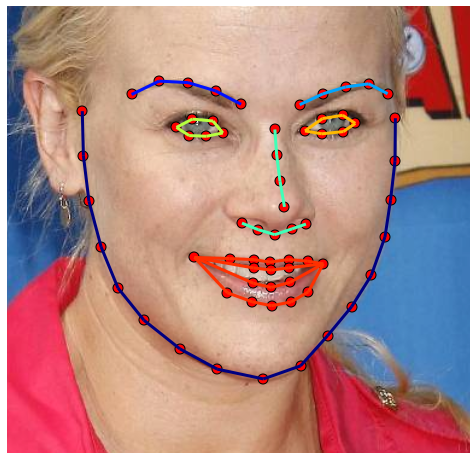
\includegraphics[width=0.16\textwidth]{figures/img0.png}
	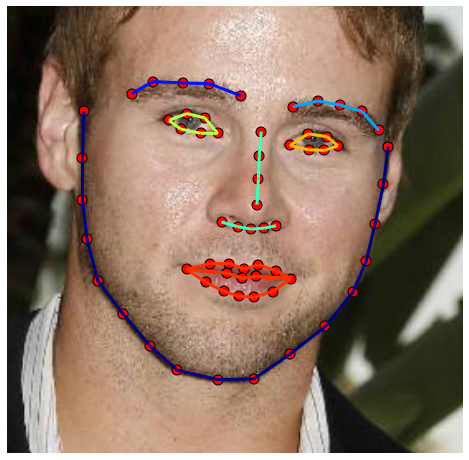
\includegraphics[width=0.16\textwidth]{figures/img1.png}
	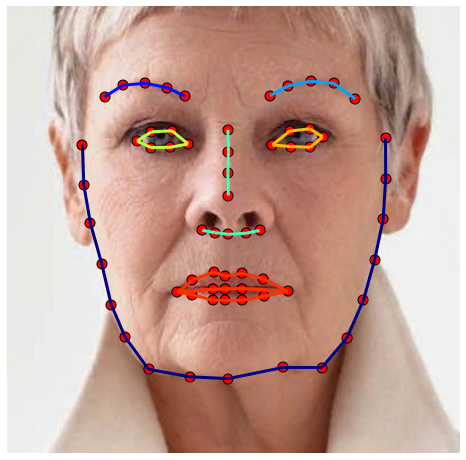
\includegraphics[width=0.16\textwidth]{figures/img2.png}
	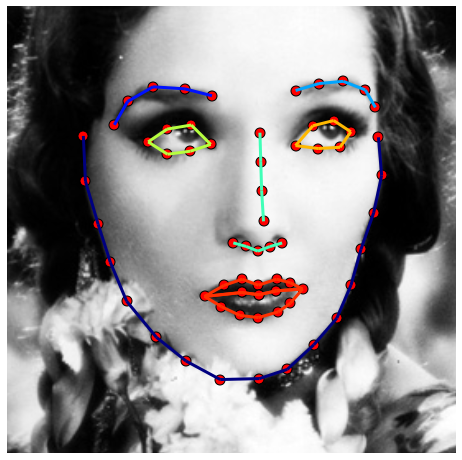
\includegraphics[width=0.16\textwidth]{figures/img3.png}
	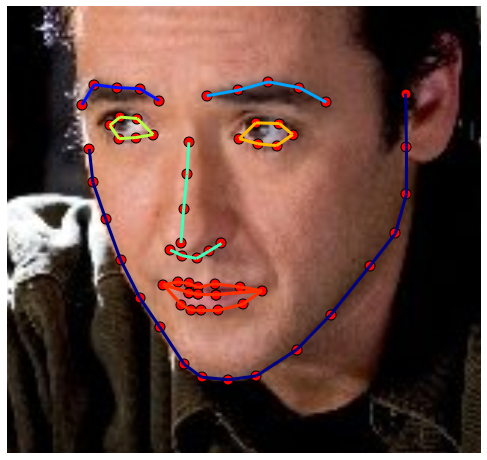
\includegraphics[width=0.16\textwidth]{figures/img4.png}
	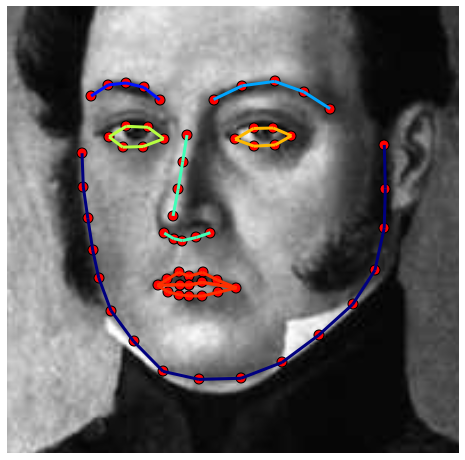
\includegraphics[width=0.16\textwidth]{figures/img5.png}
	\caption{Exemplar images from the Labeled Faces in-the-Wild (LFPW) dataset \cite{Belhumeur2011} for which a consistent set of sparse landmarks representing the shape of the object being model (human face) has been manually defined.}
	\label{fig:lfpw_images}
\end{figure*}

Active Appearance Models (AAMs) \cite{Cootes2001,Matthews2004} are generative parametric models that explain visual variations, in terms of shape and appearance, within a particular object class. AAMs are built from a collection of images for which the spatial position of a sparse set of landmark points $\mathbf{x}_i = (x_i, y_i)^T \in \mathcal{R}^2$ representing the shape $\mathbf{s} = (x_1, y_1, \dots, x_v, y_v)^T \in \mathcal{R}^{2v \times 1}$ of the object being modeled have been manually defined a priori. 

AAMs are themselves composed of three different models:
\begin{inparaenum}[(i)]
	\item shape model; 
	\item appearance model; and
	\item motion model. 
\end{inparaenum} 

The shape model, which is also referred to as Point Distribution Model (PDM), is obtained by typically applying Principal Component Analysis (PCA) to the set of object's shapes. The resulting shape model is mathematically expressed as:
\begin{equation}
	\begin{aligned}
		\mathbf{s} & = \mathbf{\bar{s}} + \sum_{i=1}^n p_i \mathbf{s}_i 
        \\
        & = \mathbf{\bar{s}} + \mathbf{S} \mathbf{p}
	\end{aligned}
\end{equation}
where $\mathbf{\bar{s}} \in \mathcal{R}^{2v \times 1}$ is the mean shape, and $\mathbf{S} \in  \mathcal{R}^{2v \times  n}$ and $\mathbf{p} \in \mathcal{R}^{n \times 1}$ denote the shape bases and shape parameters, respectively. In order to allow a particular shape instance $\mathbf{s}$ to be arbitrarily positioned in space, the previous model can be augmented with a global similarity transform. Note that this normally requires the initial shapes to be normalized with respect to the same type of transform (typically using Procrustes Analysis (PA)) before PCA is applied. This results in the following expression for each landmark point of the shape model:
\begin{equation}
	\begin{aligned}
		\mathbf{x}_i & = s \mathbf{R} \left( \mathbf{\bar{x}}_i + \mathbf{X}_i \mathbf{p} \right) + \mathbf{t}
	\end{aligned}
\end{equation}
where $s$, $\mathbf{R} \in \mathcal{R}^{2 \times 2}$ and $\mathbf{t} \in \mathcal{R}^2$  denote the scale, rotation and translation applied by the global similarity transform, respectively. Using the orthonormalization procedure described in \cite{Matthews2004} the final expression for the shape model can be compactly written as the linear combination of a set of bases:
\begin{equation}
	\begin{aligned}
		\mathbf{s} & = \mathbf{\bar{s}} + \sum_{i=1}^4 p^*_i \mathbf{s}^*_i + \sum_{i=1}^n p_i \mathbf{s}_i 
        \\
        & = \mathbf{\bar{s}} + \mathbf{S} \mathbf{p}
	\end{aligned}
    \label{eq:shape_model}
\end{equation}
where $\mathbf{S} = (\mathbf{s}^*_1, \dots, \mathbf{s}^*_4, \mathbf{s}_1, \cdots, \mathbf{s}_n) \in \mathcal{R}^{2v \times (n+4)}$ and $\mathbf{p} = (p^*_1, \dots, p^*_4, p_1, \dots, p_n)^T \in \mathcal{R}^{(n+4) \times 1}$ are redefined as the concatenation of the similarity bases $\mathbf{s}^*_i$ and similarity parameters $p^*_i$ with the original $\mathbf{S}$ and $\mathbf{p}$, respectively.

The appearance model is obtained by warping the original images onto a common reference frame (typically defined in terms of the mean shape $\mathbf{\bar{s}}$) and applying PCA to the obtained warped images. Mathematically, the appearance model is defined by the following expression:
\begin{equation}
	\begin{aligned}
		A(\mathbf{x}) & = \bar{A}(\mathbf{x}) + \sum_{i=1}^m c_i A_i(\mathbf{x})
	\end{aligned}
    \label{eq:app_model}
\end{equation}
where $\mathbf{x} \in \Omega$ denote all pixel positions on the reference frame, and $\bar{A}(\mathbf{x})$, $A_i(\mathbf{x})$ and $c_i$ denote the mean texture, the appearance bases and appearance parameters, respectively. Denoting $\mathbf{a} = \text{vec}(A(\mathbf{x}))$ as the vectorized version of the previous appearance instance, Equation \ref{eq:app_model} can be concisely written in vector form as:
\begin{equation}
	\begin{aligned}
		\mathbf{a} & = \mathbf{\bar{a}} + \mathbf{A} \mathbf{c}
	\end{aligned}
    \label{eq:app_model_vec}
\end{equation}
where $\mathbf{a} \in \mathcal{R}^{F \times 1}$ is the mean appearance, and $\mathbf{A} \in  \mathcal{R}^{F \times  m}$ and $\mathbf{c} \in \mathcal{R}^{m \times 1}$ denote the appearance bases and appearance parameters, respectively.

The role of the motion model, denoted by $\mathcal{W}(\mathbf{x}; \mathbf{p})$, is to extrapolate the position of all pixel positions $\mathbf{x} \in \Omega$ from the reference frame to a particular shape instance $\mathbf{s}$ (and vice-versa) based on their relative position with respect to the sparse set of landmarks defining the shape model (for which direct correspondences are always known). Classic motion models for AAMs are PieceWise Affine (PWA) \cite{Cootes2004,Matthews2004} and Thin Plate Splines (TPS) \cite{Cootes2004,Papandreou2008} warps. 

Given an image $I(\mathbf{x})$ containing the object of interest, its manually annotated ground truth shape $\mathbf{s}$, and a particular motion model $\mathcal{W}(\mathbf{x}, \mathbf{p})$; the two main assumptions behind AAMs are:

\begin{enumerate}
	\item The ground truth shape of the object can be well approximated by the shape model
	\begin{eqnarray}
		\begin{aligned}
			\mathbf{s} & \approx \mathbf{\bar{s}} + \mathbf{S} \mathbf{p}
		\end{aligned}
	    \label{eq:aam_1}
	\end{eqnarray}

	\item The object's appearance can be well approximated by the appearance model after the image is warped, using the motion model and the previous shape approximation, onto the reference frame:
	\begin{eqnarray}
		\begin{aligned}
			\mathbf{i}[\mathbf{p}] & \approx \mathbf{\bar{a}} + \mathbf{A} \mathbf{c} 
		\end{aligned}
	    \label{eq:aam_2}
	\end{eqnarray}
	where $\mathbf{i}[\mathbf{p}] = \mathrm{vec}(I(\mathcal{W}(\mathbf{x}; \mathbf{p}))$ denotes the vectorized version of the warped image. Note that, the warp $\mathcal{W}(\mathbf{x}; \mathbf{p})$ which explicitly depends on the shape parameters $\mathbf{p}$, relates the shape and appearance models and is a central part of the AAMs formulation
\end{enumerate}

Because of their explicit use of the motion model, the two previous assumptions provide a concise and unambiguous way to define AAMs. These assumption will be used in next section \ref{sec:probabilistic_aam} to introduce a more general and probabilistic formulation of AAMs. At this point, it is worth mentioning that the vector notation of Equations \ref{eq:aam_1} and \ref{eq:aam_2} will be, in general, the preferred notation in this paper.

% \begin{figure*}
% 	\centering
% 	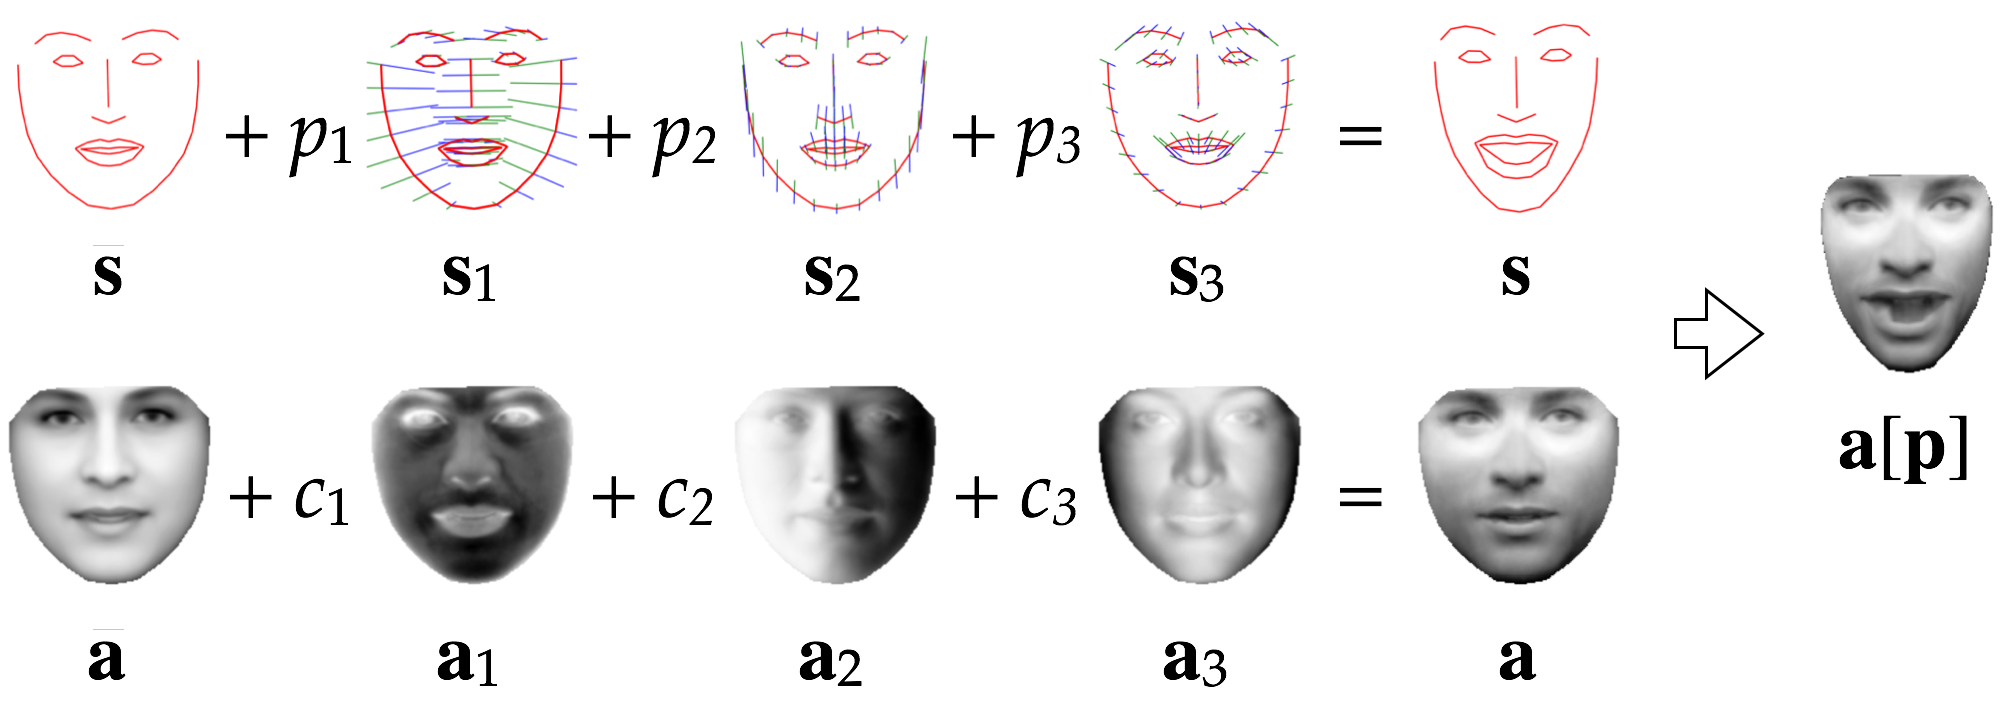
\includegraphics[width=1\textwidth]{figures/AAMs.png}
% 	\caption{Exemplar images from the Labeled Faces in-the-Wild (LFPW) dataset \cite{Belhumeur2011} for which a consistent set of sparse landmarks representing the shape of the object being model (human face) has been manually defined.}
% 	\label{fig:aams}
% \end{figure*}
%\subsection{Image Representation}
\label{sec:appearance}

AAMs have been often criticized due to their inability to generalize well under novel/unseen appearance variations. In fact, some authors \cite{Gross2005, vanderMaaten2010} argued that a low rank gaussian distribuition (as defined by a single linear model of appearance) in the intensity domain is unlikely to have sufficient modeling power to accurately capture the structure of the complex non-linear manifolds defining the appearance of most objects.

However, recent works \cite{Tzimiropoulos2013, Alabort2014, Tzimiropoulos2014, Kossaifi2014} have shown that the previous is not necessary true if the linear appearance model is learned from a rich distribution of training samples. In particular, Tzimiropoulos and Pantic \cite{Tzimiropoulos2013} showed that, for the specific case of faces, a single linear model of appearance  in the intensity domain can effectively reconstruct novel/unseen images with similar characteristics to those from which the model was learned from. 

On the other hand, a number of authors \cite{Cootes2001b,Kittipanya2006,Langs2006,Zhou2010,Lucey2013,Tzimiropoulos2012,Tzimiropoulos2014,Antonakos2014} have shown that the use of richer and more descriptive image representations can greatly improve the generalization capabilities of AAMs. The basic idea behind the majority of these works consists of creating multi-channel image representations of the original single-channel intensity images by computing \emph{dense} feature descriptors at each pixel. A linear model of appearance can be directly learned on this new multi-channel representation. Antonakos et al. \cite{Antonakos2014} have recently shown that, by using highly engineered feature descriptors such as Dense Scale Invariant Feature Transform (DSIFT) \cite{Lowe1999,Ce2011} or a dense version of Histograms of Oriented Gradients (HOG) \cite{Dalal2005}, this approach leads to state-of-the-art results in the problem of face alignment in-the-wild. Note that, as noted in their paper, this increase in generalitzation comes with a significant increases in computational cost.

In this paper, we present a complete evaluation of AAMs with respect to different fitting strategies rather than different appearance representations and, consequetly, we will limit the number of different appearance representations used to only two: (i) raw intensity and (ii) DSIFT. 

For a detailed review and performance evaluation of the latest image representations used in AAMs the interested reader is referred to \cite{Antonakos2014}.
%\subsection{Motion Model}
\label{sec:motion}

The motion model relates the shape and appearance models of an AAM by means of a particular warping functions. Recall here that the appearance model is solely defined in the
domain $\Omega$ of pixel positions in the reference frame. The role of the motion model is to extrapolate the position these pixel locations, $\mathbf{x} \in \Omega$, from the reference frame to a particular shape instance $\mathbf{s}$, and vice-versa, based on their relative position with respect to the sparse set of landmarks defining the shape model (for which direct correspondences are always known).

\subsubsection{Non-linear}

The most commonly used motion models for AAMs are Piece Wise Affine (PWA) \cite{Cootes2004,Matthews2004} and Thin Plate Splines (TPS) \cite{Cootes2004,Papandreou2008} warps.

Given two shapes in correspondance and a shared triangulation of their vertices, PWA describes the differences between the positions of their vertices as independent local affine transformations between corresponding triangles pairs. Consequently, any arbitrary point $\mathbf{x}$ on a particular triangle of one of the shapes can be directly mapped to its paired triangle on the other shape by using the affine transform relating both triangles. Excellent descriptions of PWA and their application to AAMs can be found in \cite{Cootes2004} and \cite{Matthews2004}.

On the other hand, TPS defines the mapping of arbitrary points $\mathbf{x}$ from on shape to the other as a globally smooth warp that can be expressed as a generalized linear model \cite{Bookstein1989}. For further details regarding TPS and their application to AAMs the reader is referred to \cite{Cootes2004} and \cite{Papandreou2008}.

Note that, PWA and TPS are both non-linear motion models 

bla, bla, bla... for which operations such composition and inversion are not well defined.


Figure \ref{fig:} compares the results obtained by warping using PWA and TPS on two different examples.

\subsubsection{Linear}

Amberg et al. \cite{Amberg2009} introduced a procedure for approximating the previous non-linear motion models using a simple linear model of the form:

\begin{equation}
	\begin{aligned}
		\mathbf{x} = \bar{\mathbf{x}} + \mathbf{U} \mathbf{p}
	\end{aligned}
    \label{eq:subspace_warp}
\end{equation}

where ... The idea is to learn the mean $\mathbf{x} \in \mathcal{R}^{F \times 1}$ and the subspace $\mathbf{U}\in \mathcal{R}^{F \times n}$ using training data. 

The procedure is simple and consists of two basic steps: (i) mapping the position of all pixels on the reference frame to the annotated training images using either PWA or TPS, and (ii) applying PCA to the result of the previous mapping. 

Note that, once $\mathbf{x} \in \Omega$ have been mapped onto the training images, the positions $\mathbf{x}'$ to which their are mapped onto each training image can be viewed as a dense set of manual annotations. By applying PCA on these dense annotationa we are, in fact, defining a new dense shape model for which a one to one correspondence between all of its landmarks and all the pixel positions on the reference frame exist. Consequently the position of an arbitrary pixel position $\mathbf{x}$ on the reference frame can be directly mapped onto a particular shape instance (and  vice-versa) through the explicit correspondandes given by the shape model.

Note that, the expression in equation \ref{} constitutes a true linear warp for which...

\subsubsection{Parts Translation}

As noted in Section \ref{sec:intro}, several authors \ref{} have argued that a parts-based representation of the object appearance, obtained by directly sampling the local image region around each of the landmark points defining the object's shape, is more appropriate to solve the object alignment problem. This idea was first introduce by bla, bla... in \cite{} and later developed into the field of Parts-Based Deformable Models.

Building upon the original work of \cite{}, Tzimiropoulos and Pantic \cite{} recently proposed a novel deformable model, for the specific task of face alignemnt, coined Gauss-Newton Deformable Part Model, that bares loads of similarities with the AAMs descrived in this paper. In fact, we argue that their model can be viewed as an AAM using a parts-based translational motion model.

This motion model defines the position of each pixel on the reference frame, $\mathbf{x} \in \mathbf{\Omega}$, relative to the landmark points $\mathbf{x}_i$ defining the shape of the object. Given a particular landmark point $\mathbf{x}_i$ in the reference frame its associated $\mathbf{x} \in \mathbf{\Omega}_{\mathbf{x}_i}$ are uniquily definined by the vector $\delta \boldsymbol{\ell} = \mathbf{x} - \mathbf{x}_i = (\delta x, \delta y)^T$. Consequently, the position of each pixel in the reference frame can be mapped to any arbitrary shape instance $\mathbf{s}$ by simply adding the appropriate vectors $\delta \mathbf{\ell}$ to its landmarks points appropriately

Note that the previous motion model can be defined in terms of the shape model using the following expresison

\begin{equation}
	\begin{aligned}
		\mathbf{x} & = 
        	\begin{pmatrix}
				\delta x_{1,1}
                \\
                \delta y_{1,1}
                \\ 
                \vdots
				\\ 
                \delta x_{1,k}
                \\
                \delta x_{1,k}
                \\
                \vdots
				\\ 
                \delta x_{v,1}
                \\
                \delta y_{v,1}
                \\ 
                \vdots
				\\ 
                \delta x_{v,k}
                \\
                \delta x_{v,k}
			\end{pmatrix} 
            + 
            \begin{pmatrix}
				\mathbf{M}_1 & \cdots & \mathbf{0}
                \\
                \vdots & \ddots & \vdots
                \\
                \mathbf{0} & \cdots & \mathbf{M}_v
			\end{pmatrix} \left(\bar{\mathbf{s}} + \mathbf{S} \mathbf{p} \right)
	\end{aligned}
    \label{eq:subspace_warp}
\end{equation}


where in this case x takes


Note that, AAMs using parts translational motion models are built using the exact same procedure used  as those using other type of warps. Moreover, they can also be fitted to novel images using all the all the existent AAMs fitting algorithms with no modification.


%\subsection{Factor Analysis}
\label{sec:CA}

Principal Component Analysis (PCA) \cite{} has been the most widely used CA technique to define the shape and appearance models used in AAMs \cite{}. However, the AAM definition introduced in section \ref{sec:aam} is broad enough to allow the use of other CA techniques to define such models. 

In fact, several authors have proposed the use of other CA techniques \cite{DelaTorre2008, Hamsici2009,Gonazalez2007} to define such models. On the other hand, probabilistic versions of PCA have also been used to motivate probabilistic formulations of AAMs

In this section we briefly review both PCA and Probabilistic PCA (PPCA). Note that in Section \ref{sec:paam} we will borrow key concepts from PPCA and other Probabilistic CA techniques in order to motivate and extend previous probabilistic formulation of AAMs.

%----------

\subsubsection{Principal Component Analysis}
\label{sec:PCA}

PCA finds a set of orthonormal projection bases $\mathbf{U}$ so that the latent space $\mathbf{Y}$ is the projection of the mean-centered training samples $\mathbf{\bar{X}} = \left( \mathbf{x}_1 - \bar{\mathbf{x}}, \ldots, \mathbf{x}_N - \bar{\mathbf{x}} \right)$ onto $\mathbf{U}$ (i.e. $\mathbf{Y} = \mathbf{U}^T \mathbf{\bar{X}}$). 

The optimization problem is defined as follows

\begin{equation}
	\mathbf{U}_o = \underset{\mathbf{U}}{\mathrm{arg\,max\;}} \mathrm{Tr} \left( \mathbf{U}^T \mathbf{S} \mathbf{U} \right), \,\, \mbox{s.t.} \,\, \mathbf{U}^T\mathbf{U} = \mathbf{I}
\end{equation}

where $\mathbf{S} = \frac{1}{N} \sum_{n=1}^N (\mathbf{x}_n - \bar{\mathbf{x}})(\mathbf{x}_n - \bar{\mathbf{x}})^T = \frac{1}{N} \mathbf{\bar{X}} \mathbf{\bar{X}}^T$ is the total scatter matrix and $\mathbf{I}$ is the identity matrix. 

The optimal projection bases $\mathbf{U}_o \in \mathcal{R}^{F \times M}$ are recovered by keeping the $M$ eigenvectors $\mathbf{U} = (\mathbf{u}_1, \ldots ,\mathbf{u}_M)$ that correspond to the $M$ largest eigenvalues of $\mathbf{S}$ (in the following we will assume that the eigenvalues are stored in a diagonal matrix $\mathbf{\Sigma}= \textrm{diag} \left( \lambda_1, \ldots, \lambda_M \right)$).

%----------

\subsubsection{Probabilistic PCA}
\label{sec:PPCA}

Probabilistic versions of PCA (PPCA) were independently proposed in \cite{Moghaddam1997,Roweis1998,Tipping1999} \footnote{In particular the Maximum Likelihood (ML)  solutions where provided  in \cite{Moghaddam1997,Tipping1999}, while Expectation Maximization (EM) solutions where presented in \cite{Roweis1998, Tipping1999}}. In these works the following probabilistic generative model was defined:

\begin{equation}
	\begin{aligned}
		\mathbf{x}_i & = \mathbf{W}\mathbf{y}_i + \bar{\mathbf{x}} + \boldsymbol{\epsilon}
		\\
		\mathbf{y} & \sim \mathcal{N}(\mathbf{0},\boldsymbol{\mathbf{I}}) 
		\\
		\boldsymbol{\epsilon} & \sim \mathcal{N}(\mathbf{0},\sigma^2\mathbf{I})
	\end{aligned}
	\label{eq:ppca_model}
\end{equation}

where $\mathbf{W}$ is the matrix that relates the latent variables $\mathbf{y}$ with the observed sample $\mathbf{x}$ and $\boldsymbol{\epsilon}$ is the sample noise which is assumed to be an isotropic Gaussian. The motivation is that, when $N < F$, the latent variables will offer a more compact representation of the dependencies between the observations. Denoting the parameters as $\theta = \left\{ \mathbf{W}, \bar{\mathbf{x}}, \sigma^2 \right\}$, the posterior probability over the latent variables is given by

\begin{equation}
p(\mathbf{y} | \mathbf{x}, \theta) = \mathcal{N} \left( \mathbf{M}^{-1} \mathbf{W}^T (\mathbf{x} - \bar{\mathbf{x}}), \sigma^2 \mathbf{M}^{-1} \right))
\end{equation}

where $\mathbf{M} = \mathbf{W}^T\mathbf{W} + \sigma^2 \mathbf{I}$ (note that here the bases $\mathbf{W}$ are not required to be orthonormal). Using a Maximum Likelihood (ML) approach the parameters $\theta$ are found by solving

\begin{equation}
	\begin{aligned}
		\theta_o & = \underset{\theta}{\mathrm{arg\,min\;}} \ln \prod_{i=1}^n p(\mathbf{x}_i|\theta)
		\\
		& = \underset{\theta}{\mathrm{arg\,min\;}} \ln \prod_{i=1}^n \int_{\mathbf{y}} p(\mathbf{x}_i|\mathbf{y},\theta) p(\mathbf{y}) d\mathbf{y}.
	\end{aligned}
\end{equation}

with the optimal $\mathbf{W}$, $\bar{\mathbf{x}}$ and $\sigma^2$ given by

\begin{equation}
	\begin{aligned}
		\mathbf{W} & = \mathbf{U} (\mathbf{\Sigma} - \sigma^2 \mathbf{I})^{1/2} \mathbf{R} 
		\\
		\bar{\mathbf{x}} & = \frac{1}{N} \sum_{i=1}^N \mathbf{x}_i
		\\
		\mathbf{\sigma}^2 & = \frac{1}{N-M} \sum_{i=M+1}^N \lambda_i
	\end{aligned}
\end{equation}

where $\mathbf{R}$ is an arbitrary $M \times M$ orthogonal matrix.

An alternative to the ML approach is to use an Expectation Maximization (EM) procedure where the first and second order moments of the latent space ($\mathbf{E}[\mathbf{y}]$ and $\mathbf{E}[\mathbf{y} \mathbf{y}^T]$) are also found.
The EM solutions for the parameters can be found in \cite{bishop2006pattern, tipping1999probabilistic}. Several variations of probabilistic PCA have been proposed, e.g. by incorporating sparseness and nonnegative constraints \cite{guan2009sparse} or changing the Gaussian models for others (such as the Student-t model of \cite{khan2004robust}).

\subsection{Probabilistic Formulation}
\label{sec:probabilistic_aam}

A probabilistic interpretation of AAMs can be obtained by rewriting equations \ref{eq:aam_1} and \ref{eq:aam_2} assuming probabilistic generative models for shape and appearance generation. In this paper, motivated by seminal works on Probabilistic Component Analysis (PPCA) and object tracking \cite{Tipping1999, Roweis1998, Moghaddam1997}, we will assume probabilistic models for shape and appearance generation with both Gaussian noise and Gaussian priors over the latent shape and appearance spaces\footnote{Notice that this formulation is general and one could assume other probabilistic generative models \cite{vanderMaaten2010, Bach2005, Prince2012, Nicolau2014} to define novel probabilistic versions of AAMs.}:
\begin{equation}
	\begin{aligned}
		\mathbf{s} & = \bar{\mathbf{s}} + \mathbf{S} \mathbf{p} + \boldsymbol{\varepsilon}
		\\
		\mathbf{p} & \sim \mathcal{N} \left( \mathbf{0}, \mathbf{\Lambda} \right) 
		\\
		\boldsymbol{\varepsilon} & \sim \mathcal{N} \left( \mathbf{0}, \rho^2 \mathbf{I} \right) 
	\end{aligned}
\end{equation}
\begin{equation}
	\begin{aligned}
		\mathbf{i}[\mathbf{p}] & = \bar{\mathbf{a}} + \mathbf{A} \mathbf{c} + \boldsymbol{\epsilon}
		\\
		\mathbf{c} & \sim \mathcal{N} \left( \mathbf{0}, \mathbf{\Sigma} \right) 
		\\
		\boldsymbol{\epsilon} & \sim \mathcal{N} \left( \mathbf{0}, \sigma^2 \mathbf{I} \right) 
	\end{aligned}
\end{equation}
where $\mathbf{\Lambda}$ and $\mathbf{\Sigma}$ are diagonal matrices containing the eigenvalues associated to shape and texture bases and where $\rho$ and $\sigma$ denote the estimated shape and image noises respectively.

This probabilistic formulation will be used to derive the well defined Maximum A Posteriori (MAP) and Bayesian cost functions for fitting AAMs presented in Sections \ref{sec:rssd} and \ref{sec:rpo}.

% This probabilistic formulation can be used to derive Maximum A Posteriori (MAP) version of all the existent AAMs fitting algorithms reviewed in this paper and it is an essential part of the derivation of the Bayesian inference algorithms for fitting AAMs \cite{Alabort2014} described in in Section \cite{sec:bayes}.

\section{Fitting Active Appearance Models}
\label{sec:fitting}

AAM fitting is typically formulated as a search over the shape and appearance parameters that minimize the \emph{Sum of Squared pixel Differences} (SSD) between the warped input image and the linear appearance model:
\begin{equation}
    \begin{aligned}
        \mathbf{p}_o, \mathbf{c}_o & = \underset{\mathbf{p}, \mathbf{c}}{\mathrm{arg\,min\;}} \frac{1}{2} \mathbf{r}^T\mathbf{r}
        \\
        & = \underset{\mathbf{p}, \mathbf{c}}{\mathrm{arg\,min\;}} 
        \frac{1}{2} \left\| \mathbf{i}[\mathbf{p}] - \left( \bar{\mathbf{a}} + \mathbf{A} \mathbf{c} \right) \right\|^2 
    \label{eq:ssd}
    \end{aligned}
\end{equation}

Several techniques have been proposed to solve the non-linear\footnote{Notice that the residual $\mathbf{r}$ in Equation \ref{eq:ssd} is linear with respect to the appearance parameters $\mathbf{c}$ and non-linear with respect to the shape parameters $\mathbf{p}$ through the warp $\mathcal{W}(\mathbf{x}; \mathbf{p})$.} minimization problem defined by Equation \ref{eq:ssd}. In this paper, we will center the discussion around Compositional Gradient Descent (CGD) algorithms \cite{Matthews2004, Gross2005, Papandreou2008, Amberg2009, Martins2010, Tzimiropoulos2013, Kossaifi2014} for fitting AAMs. Consequently, we will not review regression based approaches. For more details on this type of methods the interested reader is referred to the existent literature \cite{Cootes2001, Hou2001, Batur2005, Donner2006, Liu2009, Saragih2009, Tresadern2010, Sauer2011}.

The following subsections present a unified and complete view of CGD algorithms by classifying them with respect to their three main characteristics: 
\begin{inparaenum}[\itshape a\upshape)]
\item \emph{cost function} (Section \ref{sec:cost_function}); 
\item type of \emph{composition} (Section \ref{sec:composition}); and 
\item \emph{optimization method} (Section \ref{sec:optimization}).
\end{inparaenum}

% In order to accurately describe and study CGD algorithms our discussion will be divided in three different sections. In the first section we will introduce the most significant cost functions used to fit AAMs. In the second section we will introduce different types of compositions. In the third section we will present different algorithms to optimize the cost functions. Finally, in the fourth section we will relate the proposed compositional gradient descent framework to the extensive prior work on the subject. 


% \subsection{Compositional Gauss-Newton}
% \label{sec:cgd}
% Assuming, for the time being, that the true appearance parameters $\mathbf{c}_o$ are known, the problem defined by Eq. \ref{eq:ssd} reduces to a non-rigid image alignment problem \cite{Baker2004, Munoz2014} between a particular instance of the object present in the image and its optimal appearance reconstruction by the appearance model:
% \begin{equation}
%     \begin{aligned}
%         \mathbf{p}_o & = \underset{\mathbf{p}}{\mathrm{arg\,min\;}} 
%         \left\| \mathbf{i}[\mathbf{p}] - \mathbf{a} \right\|^2 
%     \label{eq:ssd_shape}
%     \end{aligned}
% \end{equation}
% where $\mathbf{a} = \bar{\mathbf{a}} + \mathbf{A} \mathbf{c}_o$ is obtained by directly evaluating Eq. \ref{eq:app_model} given the true appearance parameters $\mathbf{c}_o$.

% Compositional Gauss-Newton algorithms solve the previous non-linear optimization problem with respect to the shape parameters $\mathbf{p}$ by:
% \begin{enumerate}
%     \item Introducing an incremental warp $\mathcal{W}(\mathbf{x}; \delta \mathbf{p})$; either on the image side:
%     \label{it:step_1}
%     \begin{equation}
%         \begin{aligned}
%             \delta \mathbf{p}_o & = \underset{\delta \mathbf{p}}{\mathrm{arg\,min\;}} \left\| \mathbf{i} [\mathbf{p} \circ \delta \mathbf{p}] - \mathbf{a} \right\|^2 
%         \label{eq:fc}
%         \end{aligned}
%     \end{equation}
%     in what is known as \emph{Forward Composition} (FC) or on the model side: 
%     \begin{equation}
%         \begin{aligned}
%             \delta \mathbf{p}_o = \underset{\delta \mathbf{p}}{\mathrm{arg\,min\;}}  \left\| \mathbf{i} [\mathbf{p}] - \mathbf{a}[\delta \mathbf{p}] \right\|^2 
%         \label{eq:ic}
%         \end{aligned}
%     \end{equation}
%     in what is known as \emph{Inverse Composition} (IC).
    
%     \item Performing a Taylor expansion of the residual around the incremental warp
%     \begin{equation}
%         \begin{aligned}
%             \delta \mathbf{p}_o & = \underset{\delta\mathbf{p}}{\mathrm{arg\,min\;}} \left\| \mathbf{r}(\mathbf{p}) + \frac{\partial\mathbf{r}}{\partial\mathbf{p}} \delta\mathbf{p} \right\|^2
%             \\
%             & = \underset{\delta\mathbf{p}}{\mathrm{arg\,min\;}} \left\| \mathbf{i} [\mathbf{p}] - \mathbf{a} + \mathbf{J} \delta \mathbf{p} \right\|^2
%         \label{eq:taylor}
%         \end{aligned}
%     \end{equation}
%     where $\mathbf{J} = \nabla \mathbf{i}[\mathbf{p}] \frac{\partial\mathcal{W}}{\partial\mathbf{p}}$ or $\mathbf{J} = -\nabla \mathbf{a} \frac{\partial\mathcal{W}}{\partial\mathbf{p}}$ depending on whether forward or inverse composition is used.
    
%     \item Solving for $\delta\mathbf{p}$ by equating the derivative of Eq. \ref{eq:taylor} to $\mathbf{0}$:
%     \begin{equation}
%         \begin{aligned}
%             \frac{\partial \left\| \mathbf{r}(\mathbf{p}) + \frac{\partial\mathbf{r}}{\partial\mathbf{p}} \delta\mathbf{p} \right\|^2}{\partial \mathbf{p}} & = \mathbf{0} 
%             \\
%             \left(\mathbf{r}(\mathbf{p}) + \frac{\partial\mathbf{r}}{\partial\mathbf{p}} \delta\mathbf{p} \right) \frac{\partial\mathbf{r}}{\partial\mathbf{p}}^T  & = \mathbf{0} 
%             \\
%             \frac{\partial\mathbf{r}}{\partial\mathbf{p}}^T \mathbf{r}(\mathbf{p}) + \frac{\partial\mathbf{r}}{\partial\mathbf{p}}^T \frac{\partial\mathbf{r}}{\partial\mathbf{p}} \delta\mathbf{p} & = \mathbf{0} 
%         \label{eq:taylor}
%         \end{aligned}
%     \end{equation}
%     Rearranging, the optimal solution $\delta\mathbf{p}_o$ is given by:
%     \begin{equation}
%         \begin{aligned}
%             \delta\mathbf{p}_o & = - \left( \frac{\partial\mathbf{r}}{\partial\mathbf{p}}^T \frac{\partial\mathbf{r}}{\partial\mathbf{p}} \right)^{-1} \frac{\partial\mathbf{r}}{\partial\mathbf{p}}^T \mathbf{r}(\mathbf{p})
%             \\
%             & = - \mathbf{H}^{-1} \mathbf{J}^T \left( \mathbf{i}[\mathbf{p}] - \mathbf{a} \right)
%         \label{eq:solve_dp}
%         \end{aligned}
%     \end{equation}
    
%     \item Updating the current estimate of the warp using one of the following update rules
%     \begin{equation}
%         \mathcal{W}(\mathbf{x}; \mathbf{p}_o) \leftarrow \mathcal{W}(\mathbf{x}; \mathbf{p}) \circ \mathcal{W}(\mathbf{x}; \delta \mathbf{p}_o) 
%         \label{eq:fc_update}
%     \end{equation}
%     for forward composition and
%     \begin{equation}
%         \mathcal{W}(\mathbf{x}; \mathbf{p}_o) \leftarrow \mathcal{W}(\mathbf{x}; \mathbf{p}) \circ \mathcal{W}(\mathbf{x}; \delta \mathbf{p}_o)^{-1} 
%         \label{eq:ic_update}
%     \end{equation}
%     for inverse.
    
%     \item Going back to Step \ref{it:step_1} until: 
%     \begin{equation}
%         \begin{aligned}
%             \left\| \mathbf{p}_{k+1} - \mathbf{p}_k \right\|^2 < \epsilon
%         \end{aligned}
%     \end{equation}
%     where $\epsilon$ is a small number determining the convergence of the shape parameters $\mathbf{p}$.
% \end{enumerate}
% Further details on the computation of $\frac{\partial \mathcal{W}}{\partial \mathbf{p}}$, composition $\mathcal{W}(\mathbf{x}; \mathbf{p}) \circ \mathcal{W}(\mathbf{x}; \delta \mathbf{p})$ and inversion $\mathcal{W}(\mathbf{x};\delta \mathbf{p})^{-1}$ of typical AAM motion models such as PWA and TPS warps can be found in \cite{Matthews2004, Papandreou2008}.

% In general, optimization of Eq. \ref{eq:ssd} with respect to the appearance parameters is highly dependent on the particular algorithm being used. The next subsections provide a detailed review of the main existent strategies used by compositional Gauss-Newton algorithms to deal with the appearance parameters.

% \begin{table*}
% \begin{tabular}{lccccccc}
% \hline\noalign{\smallskip}
% Algorithm& $\mathbf{a}$ & $\mathbf{J}$ & $\mathbf{J}^T\mathbf{Q}$ & $\mathbf{H}$ & $\mathbf{H}^{-1}$ & $\mathbf{J}^T\mathbf{e}$ & $\mathbf{H}^{-1}\mathbf{J}^T\mathbf{e}$ \\
% \noalign{\smallskip}\hline\noalign{\smallskip}
% PFC & - & $O(nF)$ & $O(mnF)$ & $O(n^2F)$ & $O(n^3)$ & $O(nF)$ & $O(n^2)$ \\
% PIC & - & - & - & - & - & $O(nF)$ & - \\
% SFC & $O(mF)$ & $O(nF)$ & - & $O((m+n)^2F)$ & $O((m+n)^3)$ & $O((m+n)F)$ & $O((m+n)^2)$ \\
% SIC & $O(mF)$ & $O(nF)$ & - & $O((m+n)^2F)$ & $O((m+n)^3)$ & $O((m+n)F)$ & $O((m+n)^2)$ \\
% AFC & $O(mF)$ & $O(nF)$ & - & $O(n^2F)$ & $O(n^3)$ & $O(nF)$ & $O(n^2)$ \\
% AIC & $O(mF)$ & $O(nF)$ & - & $O(n^2F)$ & $O(n^3)$ & $O(nF)$ & $O(n^2)$ \\
% Fast-SFC & - & $O(nF)$ & $O(mnF)$ & $O(n^2F)$ & $O(n^3)$ & $O(nF)$ & $O(n^2)$ \\
% Fast-SIC &  $O(mF)$ & $O(nF)$ & $O(mnF)$ & $O(n^2F)$ & $O(n^3)$ & $O(nF)$ & $O(n^2)$ \\
% \noalign{\smallskip}\hline
% \end{tabular}
% \caption{Computational cost per iteration of Compositional Gradient Descent algorithms for fitting AAMs.}
% \label{tab:complexity}  
% \end{table*}

\subsection{Cost Functions}
\label{sec:cost}

AAM fitting is defined as the regularized search over the shape and appearance parameters that minimize a global measure of similarity between the vectorized warped image and the appearance model:
\begin{equation}
    \begin{aligned}
        \mathbf{p}^*, \mathbf{c}^* & = \underset{\mathbf{p}, \mathbf{c}} {\mathrm{arg\, min\;}} \mathcal{R} (\mathbf{p}, \mathbf{c}) + \mathcal{D} (\mathbf{i}[\mathbf{p}], \mathbf{c}) 
        \end{aligned}
    \label{eq:aam_fitting}
\end{equation}
where $\mathcal{R}$ is the regularization term that penalizes complex shape and appearance deformations and $\mathcal{D}$ is the data term that
quantifies the global measure of similarity between the vectorized warped image and the appearance model.

\subsubsection{Regularized Sum of Squared Differences}
\label{sec:rssd}

Arguably, the most natural choices for the previous data and regularization terms, $\mathcal{D}$ and $\mathcal{R}$, are the \emph{Sum of Squared} pixel \emph{Differences} (SSD) between the vectorized warped image and the appearance model\footnote{Notice that this choice of $\mathcal{D}$ is very related to the second main assumption behind AAMs, Equation \ref{eq:aam_2}.} and the sum of the $\l_2^2$-norm over the shape and appearance parameters respectively:
\begin{equation}
    \begin{aligned}
        \mathbf{p}^*, \mathbf{c}^* & = \underset{\mathbf{p}, \mathbf{c}} {\mathrm{arg\, min\;}} \underbrace{||\mathbf{p}||^2 + ||\mathbf{c}||^2}_{\mathcal{R} (\mathbf{p}, \mathbf{c})} +
        \\
        & \qquad \qquad \quad \underbrace{|| \mathbf{i}[\mathbf{p}] - (\mathbf{\bar{a}} + \mathbf{A} \mathbf{c}) ||^2}_{\mathcal{D} (\mathbf{i}[\mathbf{p}], \mathbf{c})}
    \end{aligned}
    \label{eq:rssd}
\end{equation}
\subsubsection*{Probabilistic Interpretation}
\label{sec:rssd_pi}

A probabilistic interpretation of the previous cost function can be naturally derived using the probabilistic generative models of shape and appearance introduced in Section \ref{sec:prob_aam}. Denoting the model parameters as \mbox{$\Theta = \{\mathbf{\bar{s}}, \mathbf{S}, \mathbf{\Lambda}, \mathbf{\bar{a}}, \mathbf{A}, \mathbf{\Sigma}, \sigma^2\}$} and taking into account the prior distributions over the shape and texture parameters:
\begin{equation}
    \begin{aligned}
        \mathbf{p}^*, \mathbf{c}^* & = \underset{\mathbf{p}, \mathbf{c}}{\mathrm{arg\,max\;}} p(\mathbf{p}, \mathbf{c}, \mathbf{i}[\mathbf{p}] | \Theta) 
        \\
        & = \underset{\mathbf{p}, \mathbf{c}}{\mathrm{arg\,max\;}}  p(\mathbf{p} | \mathbf{\Lambda})  p(\mathbf{c} | \mathbf{\Sigma}) p(\mathbf{i}[\mathbf{p}] |
        \mathbf{p}, \mathbf{c}, \Theta)  
        \\
        & = \underset{\mathbf{p}, \mathbf{c}}{\mathrm{arg\,max\;}}  \ln p(\mathbf{p} | \mathbf{\Lambda}) + \ln p(\mathbf{c} | \mathbf{\Sigma}) +
        \\
        & \qquad \qquad \quad \ln p(\mathbf{i}[\mathbf{p}] | \mathbf{p}, \mathbf{c}, \Theta)
        \\
        & = \underset{\mathbf{p}, \mathbf{c}}{\mathrm{arg\,min\;}}  \underbrace{\frac{}{} ||\mathbf{p}||^2_{\mathbf{\Lambda}^{-1}} + ||\mathbf{c}||^2_{\mathbf{\Sigma}^{-1}}}_{\mathcal{R}(\mathbf{p}, \mathbf{c})} +
        \\
        & \qquad \qquad \quad  \underbrace{ \frac{1}{\sigma^2} || \mathbf{i}[\mathbf{p}] - (\mathbf{\bar{a}} + \mathbf{A} \mathbf{c}) ||^2}_{\mathcal{D}(\mathbf{i}[\mathbf{p}], \mathbf{c})} 
    \end{aligned}
    \label{eq:prob_rssd}
\end{equation}
where we have assumed that the shape and appearance parameters are independent \footnote{Notice that this is a common assumption in compositional gradient descent algorithms \cite{Matthews2004}, however, in reality, some degree of dependence between these parameters is to be expected \cite{Cootes2001}.}

The previous Maximum-A-Posteriori (MAP) formulation is a weighted version of the optimization problem defined by Equation \ref{eq:rssd}. The maximization of the prior probability over the shape and texture parameters led to the minimization of the regularization term $\mathcal{R}$ and the maximization of the conditional probability of the vectorized warped image given the shape, texture and model parameters led to the minimization of the data term $\mathcal{D}$.

\subsubsection{Regularized Project-Out}
\label{sec:po}

Matthews and Baker showed in \cite{Matthews2004} that one could express the SSD between the vectorized warped image and the linear texture model as the sum of two different terms:
\begin{equation}
    \begin{aligned}
        \mathbf{p}_o, \mathbf{c}_o & =  \underset{\mathbf{p}, \mathbf{c}}{\mathrm{arg\,min\;}} \mathbf{r}^T \mathbf{r} 
        \\
        & = \underset{\mathbf{p}, \mathbf{c}}{\mathrm{arg\,min\;}} \mathbf{r}^T (\mathbf{A}\mathbf{A}^T + \mathbf{I} - \mathbf{A}\mathbf{A}^T) \mathbf{r}
        \\
        & = \underset{\mathbf{p}, \mathbf{c}}{\mathrm{arg\,min\;}} \mathbf{r}^T (\mathbf{A}\mathbf{A}^T) \mathbf{r} + \mathbf{r}^T (\mathbf{I} - \mathbf{A}\mathbf{A}^T) \mathbf{r}
        \\
        & = \underset{\mathbf{p}, \mathbf{c}}{\mathrm{arg\,min\;}} \left\| \mathbf{i}[\mathbf{p}] - \left( \bar{\mathbf{a}} + \mathbf{A} \mathbf{c} \right) \right\|_{\mathbf{A}\mathbf{A}^T}^2 \, + 
        \\
        & \qquad \qquad \,\,\,\,\, \left\| \mathbf{i}[\mathbf{p}] - \left( \bar{\mathbf{a}} + \mathbf{A} \mathbf{c} \right) \right\|_{\mathbf{I} - \mathbf{A}\mathbf{A}^T}^2
    \label{eq:po_cost}
    \end{aligned}
\end{equation}
The first term defines the distance \emph{within} the learned appearance subspace and it is always $0$ regardless of the value of the shape parameters $\mathbf{p}$:
\begin{equation}
    \begin{aligned}
        f_1(\mathbf{p}, \mathbf{c}) & = \left\| \mathbf{i}[\mathbf{p}] - \left( \bar{\mathbf{a}} + \mathbf{A} \mathbf{c} \right) \right\|_{\mathbf{A}\mathbf{A}^T}^2
        \\
        & = \underbrace{\mathbf{i}[\mathbf{p}]^T \mathbf{A}}_{\mathbf{c}^T} \underbrace{\mathbf{A}^T \mathbf{i}[\mathbf{p}]}_{\mathbf{c}} - \underbrace{2\overbrace{\mathbf{i}[\mathbf{p}]^T \mathbf{A}}^{\mathbf{c}^T} \overbrace{\mathbf{A}^T \bar{\mathbf{a}}}^{\mathbf{0}}}_{0} \, - 
        \\
        & \quad \,\, 2\underbrace{\mathbf{i}[\mathbf{p}]^T \mathbf{A}}_{\mathbf{c}^T} \underbrace{\overbrace{\mathbf{A}^T \mathbf{A}}^{\mathbf{I}} \mathbf{c}}_{\mathbf{c}} + \underbrace{\overbrace{\mathbf{a}^T \mathbf{A}}^{\mathbf{0}^T} \overbrace{\mathbf{A}^T \mathbf{a}}^{\mathbf{0}}}_{0} \, +
        \\
        & \quad \,\, \underbrace{\mathbf{c}^T \overbrace{\mathbf{A}^T \mathbf{A}}^{\mathbf{I}}}_{\mathbf{c}^T} \underbrace{\overbrace{\mathbf{A}^T \mathbf{A}}^{\mathbf{I}} \mathbf{c}}_{\mathbf{c}}
        \\
        & = \mathbf{c}^T\mathbf{c} - 2\mathbf{c}^T\mathbf{c} + \mathbf{c}^T\mathbf{c}
        \\
        & = 0
    \end{aligned}
\end{equation}
The second term measures the distance \emph{to} the learned appearance subspace i.e. the distance within its orthogonal complement. After some algebraic manipulation, one can show that this term reduces to a function that only depends on the shape parameters $\mathbf{p}$:
\begin{equation}
    \begin{aligned}
        f_2(\mathbf{p}, \mathbf{c}) & = \left\| \mathbf{i}[\mathbf{p}] - \left( \bar{\mathbf{a}} + \mathbf{A} \mathbf{c} \right) \right\|_{\mathbf{Q}}^2
        \\
        & = \mathbf{i}[\mathbf{p}]^T \mathbf{Q} \mathbf{i}[\mathbf{p}] - 2\mathbf{i}[\mathbf{p}]^T \mathbf{Q} \bar{\mathbf{a}} \, - 
        \\
        & \quad \,\, \underbrace{2\mathbf{i}[\mathbf{p}]^T \mathbf{Q} \mathbf{A}\mathbf{c}}_{0} + \mathbf{a}^T \mathbf{Q} \mathbf{a} + \underbrace{\mathbf{c}^T \mathbf{A}^T \mathbf{Q} \mathbf{A}\mathbf{c}}_{0}
        \\
        & = \mathbf{i}[\mathbf{p}]^T \mathbf{Q} \mathbf{i}[\mathbf{p}] - 2\mathbf{i}[\mathbf{p}]^T \mathbf{Q} \bar{\mathbf{a}} + \mathbf{a}^T \mathbf{Q} \mathbf{a}
        \\
        & = \left\| \mathbf{i}[\mathbf{p}] - \bar{\mathbf{a}} \right\|_{\mathbf{Q}}^2
    \end{aligned}
\end{equation}
where we have defined $\mathbf{Q}= \mathbf{I} -\mathbf{A}\mathbf{A}^T$. 

Note that, as mentioned above, the previous term does not depend on the appearance parameters $\mathbf{c}$:
\begin{equation}
    \begin{aligned}
        f_2(\mathbf{p}, \mathbf{c}) & = \hat{f}_2(\mathbf{p}) = \left\| \mathbf{i}[\mathbf{p}] - \bar{\mathbf{a}} \right\|_{\mathbf{I} -\mathbf{A}\mathbf{A}^T }^2
    \label{eq:po_cost}
    \end{aligned}
\end{equation}
Therefore, the minimization problem defined by Eq. \ref{eq:po_cost} reduces to:
\begin{equation}
    \begin{aligned}
        \mathbf{p}_o & =  \underset{\mathbf{p}}{\mathrm{arg\,min\;}}  \left\| \mathbf{i}[\mathbf{p}] - \bar{\mathbf{a}} \right\|_{\mathbf{I} -\mathbf{A}\mathbf{A}^T }^2
    \label{eq:po_cost2}
    \end{aligned}
\end{equation}

\subsubsection*{Probabilistic Interpretation}
\label{sec:po_pi}

In our previous work \cite{Alabort2014}, we showed that assuming the probabilistic models of shape and appearance defined in Section \ref{} the previous project-out cost function could be naturally derived by marginalizing Equation \ref{} over the appearance parameters:

\begin{equation}
    \begin{aligned}
        \mathbf{p}^*, \mathbf{c}^* & = \underset{\mathbf{p}, \mathbf{c}}{\mathrm{arg\,max\;}} p(\mathbf{p}, \mathbf{c}, \mathbf{i}[\mathbf{p}] | \Theta) 
        \\
        & = \underset{\mathbf{p}, \mathbf{c}}{\mathrm{arg\,max\;}}  p(\mathbf{p} | \mathbf{\Lambda})  p(\mathbf{c} | \mathbf{\Sigma}) p(\mathbf{i}[\mathbf{p}] |
        \mathbf{p}, \mathbf{c}, \Theta)  
        \\
        & = \underset{\mathbf{p}, \mathbf{c}}{\mathrm{arg\,max\;}}  \ln p(\mathbf{p} | \mathbf{\Lambda}) + \ln p(\mathbf{c} | \mathbf{\Sigma}) +
        \\
        & \qquad \qquad \quad \ln p(\mathbf{i}[\mathbf{p}] | \mathbf{p}, \mathbf{c}, \Theta)
        \\
        & = \underset{\mathbf{p}, \mathbf{c}}{\mathrm{arg\,min\;}}  \underbrace{-\ln p(\mathbf{p} | \mathbf{\Lambda}) -\ln p(\mathbf{c} | \mathbf{\Sigma})}_{R(\mathbf{p}, \mathbf{c})} +
        \\
        & \qquad \qquad \quad \underbrace{-\ln p(\mathbf{i}[\mathbf{p}] | \mathbf{p}, \mathbf{c}, \Theta)}_{D(\mathcal{I}, \mathbf{p}, \mathbf{c})}
        \\
        & = \underset{\mathbf{p}, \mathbf{c}}{\mathrm{arg\,min\;}}  \underbrace{\frac{}{} ||\mathbf{p}||^2_{\mathbf{\Lambda}^{-1}} + ||\mathbf{c}||^2_{\mathbf{\Sigma}^{-1}}}_{\mathcal{R}(\mathbf{p}, \mathbf{c})} +
        \\
        & \qquad \qquad \quad  \underbrace{ \frac{1}{\sigma^2} || \mathbf{i}[\mathbf{p}] - (\mathbf{\bar{a}} + \mathbf{A} \mathbf{c}) ||^2}_{\mathcal{D}(I, \mathbf{p}, \mathbf{c})} 
    \end{aligned}
    \label{eq:prob_aam_fitting}
\end{equation}

Note that in this derivation the is comprised of two different distances: (i) the Mahalanobis distance \emph{within}
the appearance subspace W and (ii) the Euclidean distance
\emph{to} its orthogonal complement W¯ = I − WWT
weighted by the inverse of the estimated sample noise σ
2
.
The first of these distances favors solutions with higher
probability within latent subspace W, acting as a regularizer
that ensures the solution x(po) can be well reconstructed
by the texture model. The second distance captures
everything that cannot be generated by the texture model
(e.g. occlusions and other unseen variations) and weights it
with respect to the estimated sample noise 4
.
Note that, the contribution of the second term 1
σ2 ||x(p)−
m||2
I−WWT decreases as the estimated sample noise increases.
On the other hand, when the variance Λ of the
prior over the latent subspace increases (and especially as
Λ → ∞) c becomes uniformly distributed and the contribution
of the first term ||x(p) − m||2
WD−1WT vanishes.
Hence, under our Bayesian formulation, the project-out
cost function arises naturally from assuming a uniform prior over the latent texture space

\subsection{Type of Composition}
\label{sec:composition}

The optimization problems define by Equations \ref{eq:} and \ref{eq:} are both non-linear optimization

\subsubsection{Forward}
\label{sec:forward}

\begin{equation}
 	\begin{aligned}
    	\mathcal{W}(\mathbf{x}; \mathbf{p}_k^*) \leftarrow \mathcal{W}(\mathbf{x}; \mathbf{p}_{k-1}^*) \circ \mathcal{W}(\mathbf{x}; \Delta \mathbf{p}^*) 
    \label{eq:fc_update}
    \end{aligned}
\end{equation}


\subsubsection{Inverse}
\label{sec:inverse}

\begin{equation}
 	\begin{aligned}
    	\mathcal{W}(\mathbf{x}; \mathbf{p}_k^*) \leftarrow \mathcal{W}(\mathbf{x}; \mathbf{p}_{k-1}^*) \circ \mathcal{W}(\mathbf{x}; \Delta \mathbf{p}^*)^{-1} 
    \label{eq:ic_update}
    \end{aligned}
\end{equation}

\subsubsection{Asymmetric}
\label{sec:asymmetric}

\begin{equation}
 	\begin{aligned}
    	\mathcal{W}(\mathbf{x}; \mathbf{p}_k^*) \leftarrow \mathcal{W}(\mathbf{x}; \mathbf{p}_{k-1}^*) \circ \mathcal{W}(\mathbf{x}; \alpha \Delta \mathbf{p}^*)\circ \mathcal{W}(\mathbf{x}; (1-\alpha) \Delta \mathbf{p}^*) 
    \label{eq:ac_update}
    \end{aligned}
\end{equation}

\paragraph{Symmetric}
\label{sec:symmetric}

\begin{equation}
 	\begin{aligned}
    	\mathcal{W}(\mathbf{x}; \mathbf{p}_k^*) \leftarrow \mathcal{W}(\mathbf{x}; \mathbf{p}_{k-1}^*) \circ \mathcal{W}(\mathbf{x}; \frac{1}{2} \Delta \mathbf{p}^*)\circ \mathcal{W}(\mathbf{x}; \frac{1}{2} \Delta \mathbf{p}^*) 
    \label{eq:ac_update}
    \end{aligned}
\end{equation}

\subsubsection{Bidirectional}
\label{sec:bidirectional}

\begin{equation}
 	\begin{aligned}
    	\mathcal{W}(\mathbf{x}; \mathbf{p}_k^*) \leftarrow \mathcal{W}(\mathbf{x}; \mathbf{p}_{k-1}^*) \circ \mathcal{W}(\mathbf{x}; \Delta \mathbf{p}^*)\circ \mathcal{W}(\mathbf{x}; \Delta \mathbf{q}^*)^{-1} 
    \label{eq:bc_update}
    \end{aligned}
\end{equation}

\subsection{Optimization Method}
\label{sec:optimization}

Step \ref{it:step_2} and \ref{it:step_3} in CGD algorithms, i.e. linearizing the cost and solving for the incremental warp respectively, depend on the specific optimization method used by the algorithm. In this paper, we distinguish between three main optimization methods\footnote{Amberg et al. proposed the use of the \emph{Steepest Descent} method \cite{Boyd2004} in \cite{Amberg2009}. However, their approach requires a special formulation of the motion model and it performs poorly using the standard independent AAM formulation \cite{Matthews2004} used in this work.}:
\begin{inparaenum}[\itshape i\upshape)]
    \item \emph{Gauss-Newton} \cite{Boyd2004, Matthews2004, Gross2005, Martins2010, Papandreou2008, Tzimiropoulos2013};
    \item \emph{Newton} \cite{Boyd2004, Kossaifi2014}; and
    \item \emph{Wiberg} \cite{Okatani2006, Strelow2012, Papandreou2008, Tzimiropoulos2013}.
\end{inparaenum}

The previous methods can be used to iteratively solve the non-linear optimization problems defined by Equations \ref{eq:prob_rssd} and \ref{eq:prob_po}. The main differences between them are:
\begin{enumerate}
    \item The term being linearized. Gauss-Newton and Wiberg linearize the residual $\mathbf{r}$ while Newton linearizes the whole data term $\mathcal{D}$.

    \item The way in which each method solves for the incremental parameters $\Delta \mathbf{c}$, $\Delta \mathbf{p}$ and $\Delta \mathbf{q}$. Gauss-Newton and Newton can either solve for them \emph{simultaneously} or in an \emph{alternated} fashion while Wiberg defines its own procedure to solve for different sets of parameters\footnote{Wiberg reduces to Gauss-Newton when only a single set of parameters needs to be inferred.}.
\end{enumerate}

The following subsections thoroughly explain how the previous optimization methods are used in CGD algorithms. In order to simplify their comprehension full derivations will be given for all methods using the SSD data term (Equation \ref{eq:ssd}) with both asymmetric (Section \ref{sec:asymmetric}) and bidirectional (Section \ref{sec:bidirectional}) compositions\footnote{These represent the most general cases because the derivations for forward, inverse and symmetric compositions can be directly obtained from the asymmetric one and they require solving for both shape and appearance parameters.} while only direct solutions will be given for the Project-Out data term (Equation \ref{eq:po}).


\subsubsection{Gauss-Newton}
\label{sec:gauss_newton}

When \emph{asymmetric} composition is used, the optimization problem define by the SSD data term is:
\begin{equation}
    \begin{aligned}
        \Delta \mathbf{c}^*, \Delta \mathbf{p}^* & = \underset{\Delta \mathbf{c}, \Delta \mathbf{p}}{\mathrm{arg\,min\;}} \frac{1}{2} \mathbf{r}_a^T\mathbf{r}_a
    \label{eq:asymmetric_ssd}
    \end{aligned}
\end{equation}
with the asymmetric residual $\mathbf{r}_a$ defined as:
\begin{equation}
    \begin{aligned}
		\mathbf{r}_a & = \mathbf{i}[\mathbf{p} \circ \alpha \Delta \mathbf{p}] - (\mathbf{a} + \mathbf{A}(\mathbf{c} + \Delta\mathbf{c})) [\beta \Delta \mathbf{p}^{-1}]
    \label{eq:asymmetric_residual}
    \end{aligned}
\end{equation}
and where we have introduced the incremental appearance parameters $\Delta\mathbf{c}$\footnote{The value of the current estimate of appearance parameters is updated at each iteration using the following additive update rule: $\mathbf{c} \leftarrow \mathbf{c} + \Delta \mathbf{c}$}. 
The Gauss-Newton method solves the previous optimization problem by performing a \emph{first} order Taylor expansion of the residual:
\begin{equation}
    \begin{aligned}
		\mathbf{r}_a(\Delta \boldsymbol{\ell}) & \approx \hat{\mathbf{r}}_a(\Delta \boldsymbol{\ell})
		\\
		& \approx \mathbf{r}_a + \frac{\partial \mathbf{r}_a}{\partial \Delta \boldsymbol{\ell}} \Delta \boldsymbol{\ell}
    \label{eq:asymmetric_residual_taylor}
    \end{aligned}
\end{equation}
and solving the following approximation of the original problem:
\begin{equation}
    \begin{aligned}
        \Delta \boldsymbol{\ell}^* & = \underset{\Delta \boldsymbol{\ell}}{\mathrm{arg\,min\;}} \frac{1}{2} \hat{\mathbf{r}}_a^T\hat{\mathbf{r}}_a
    \label{eq:asymmetric_ssd_taylor}
    \end{aligned}
\end{equation}
where, in order to unclutter the notation, we have defined $\Delta \boldsymbol{\ell} = (\Delta \mathbf{c}^T, \Delta \mathbf{p}^T)^T$ and the partial derivative of the residual with respect to the previous parameters, i.e. the \emph{Jacobian} of the residual, is defined as:
\begin{equation}
    \begin{aligned}
		\frac{\partial \mathbf{r}_a}{\partial \Delta \boldsymbol{\ell}}& = \left( \frac{\partial \mathbf{r}_a}{\partial \Delta \mathbf{c}}, \frac{\partial \mathbf{r}_a}{\partial \Delta \mathbf{p}} \right)
		\\
		& = \left( -\mathbf{A}, \nabla \mathbf{t} \frac{\partial \mathcal{W}}{\partial \Delta \mathbf{p}} \right)
		\\
		& = \left( -\mathbf{A}, \mathbf{J}_\mathbf{t} \right)
    \label{eq:asymmetric_jacobian}
    \end{aligned}
\end{equation}
where $\nabla\mathbf{t} = \left( \alpha \nabla \mathbf{i}[\mathbf{p}]  + \beta \nabla (\mathbf{a} + \mathbf{A}\mathbf{c}) \right)$.

When \emph{bidirectional} composition is used, the optimization problem is defined as:
\begin{equation}
    \begin{aligned}
        \Delta \mathbf{c}^*, \Delta \mathbf{p}^*, \Delta \mathbf{q}^*& = \underset{\Delta \mathbf{c}, \Delta \mathbf{p}, \Delta \mathbf{q}}{\mathrm{arg\,min\;}} \frac{1}{2} \mathbf{r}_b^T\mathbf{r}_b
    \label{eq:bidirectional_ssd}
    \end{aligned}
\end{equation}
where the bidirectional residual $\mathbf{r}_b$ reduces to:
\begin{equation}
    \begin{aligned}
		\mathbf{r}_b & = \mathbf{i}[\mathbf{p} \circ \Delta \mathbf{p}] - (\mathbf{a} + \mathbf{A}(\mathbf{c} + \Delta\mathbf{c})) [\Delta \mathbf{q}]
    \label{eq:bidirectional_residual}
    \end{aligned}
\end{equation}
The Gauss-Newton method proceeds in exactly the same manner as before, i.e. performing a first order Taylor expansion:
\begin{equation}
    \begin{aligned}
		\mathbf{r}_b(\Delta \boldsymbol{\ell}) & \approx \hat{\mathbf{r}}_b(\Delta \boldsymbol{\ell})
		\\
		& \approx \mathbf{r}_b + \frac{\partial \mathbf{r}_b}{\partial \Delta \boldsymbol{\ell}} \Delta \boldsymbol{\ell}
    \label{eq:idirectional_residual_taylor}
    \end{aligned}
\end{equation}
and solving the approximated problem:
\begin{equation}
    \begin{aligned}
        \Delta \boldsymbol{\ell}^* & = \underset{\Delta \boldsymbol{\ell}}{\mathrm{arg\,min\;}} \frac{1}{2} \hat{\mathbf{r}}_b^T\hat{\mathbf{r}}_b
    \label{eq:bidirectional_ssd_taylor}
    \end{aligned}
\end{equation}
where, in this case, $\Delta \boldsymbol{\ell} = (\Delta \mathbf{c}^T, \Delta \mathbf{p}^T, \Delta \mathbf{q}^T)^T$ and the Jacobian of the residual is defined as:
\begin{equation}
    \begin{aligned}
		\frac{\partial \mathbf{r}_b}{\partial \Delta \boldsymbol{\ell}}& = \left( \frac{\partial \mathbf{r}_b}{\partial \Delta \mathbf{c}}, \frac{\partial \mathbf{r}_b}{\partial \Delta \mathbf{p}}, \frac{\partial \mathbf{r}_b}{\partial \Delta \mathbf{q}} \right)
		\\
		& = \left( -\mathbf{A}, \mathbf{J}_{\mathbf{i}}, -\mathbf{J}_{\mathbf{a}} \right)
    \label{eq:bidirectional_jacobian}
    \end{aligned}
\end{equation}
where $\mathbf{J}_\mathbf{i} = \nabla \mathbf{i}[\mathbf{p}] \frac{\partial \mathcal{W}}{\partial \Delta \mathbf{p}}$ and $\mathbf{J}_\mathbf{a} = \nabla (\mathbf{a} + \mathbf{A}\mathbf{c}) \frac{\partial \mathcal{W}}{\partial \Delta \mathbf{q}}.$


\subsubsection*{Simultaneous}
\label{sec:gauss_newton_simultaneous}

The optimization problem defined by Equations \ref{eq:asymmetric_ssd_taylor}  and \ref{eq:bidirectional_ssd_taylor} can be solved with respect to all parameters simultaneously by simply equating their derivative to $0$:
\begin{equation}
    \begin{aligned}
		0 & = \frac{\partial\frac{1}{2}\hat{\mathbf{r}}^T \hat{\mathbf{r}}}{\partial \Delta \boldsymbol{\ell}}
		\\
		& = \frac{\partial\frac{1}{2}(\mathbf{r} + \frac{\partial \mathbf{r}}{\partial \Delta \boldsymbol{\ell}} \Delta \boldsymbol{\ell})^T(\mathbf{r} + \frac{\partial \mathbf{r}}{\partial \Delta \boldsymbol{\ell}} \Delta \boldsymbol{\ell})}{\partial \Delta \boldsymbol{\ell}}
		\\
		& = \left( \mathbf{r} + \frac{\partial \mathbf{r}}{\partial \Delta \boldsymbol{\ell}} \Delta \boldsymbol{\ell} \right) \frac{\partial \mathbf{r}}{\partial \Delta \boldsymbol{\ell}}^T
    \label{eq:ssd_bc}
    \end{aligned}
\end{equation}
The solution is given by:
\begin{equation}
    \begin{aligned}
		\Delta \boldsymbol{\ell}^* & =  -\left( \frac{\partial \mathbf{r}}{\partial \Delta \boldsymbol{\ell}}^T \frac{\partial \mathbf{r}}{\partial \Delta \boldsymbol{\ell}} \right)^{-1} \frac{\partial \mathbf{r}}{\partial \Delta \boldsymbol{\ell}}^T \mathbf{r}
    \label{eq:sim_solution}
    \end{aligned}
\end{equation}
where $\left( \frac{\partial \mathbf{r}}{\partial \Delta \boldsymbol{\ell}}^T \frac{\partial \mathbf{r}}{\partial \Delta \boldsymbol{\ell}} \right)$ is known as the Gauss-Newton approximation to the \emph{Hessian} matrix.

Directly inverting $\left( \frac{\partial \mathbf{r}}{\partial \Delta \boldsymbol{\ell}}^T \frac{\partial \mathbf{r}}{\partial \Delta \boldsymbol{\ell}} \right)$ has complexity\footnote{\label{foot:complexity}$m$ and $n$ denote the number of shape and appearance parameters respectively while $F$ denotes the number of pixels on the reference frame.} $O((n + m)^3)$ for asymmetric composition and $O((2n + m)^3)$ for bidirectional composition. However, one can take advantage of the problem structure and derive an algorithm with smaller complexity by using the \emph{Schur complement}\footnote{
Applying the Schur complement to the following system of equations:
\begin{equation*}
    \begin{aligned}
        \mathbf{A} \mathbf{x} + \mathbf{B} \mathbf{y} = \mathbf{a}
        \\
        \mathbf{C} \mathbf{x} + \mathbf{D} \mathbf{y} = \mathbf{b}
    \label{eq:schur_system}
    \end{aligned}
\end{equation*}
the solution for $\mathbf{x}$ is given by:
\begin{equation*}
    \begin{aligned}
        (\mathbf{A} - \mathbf{B}\mathbf{D}^{-1}\mathbf{C}) \mathbf{x} = \mathbf{a} - \mathbf{B}\mathbf{D}^{-1}\mathbf{b}
    \label{eq:schur_system}
    \end{aligned}
\end{equation*}
and the solution for $\mathbf{y}$ is obtained by substituting the value of $\mathbf{x}$ into the original system.}
\cite{Boyd2004}.

For \emph{asymmetric} composition we have:
\begin{equation}
    \begin{aligned}
    	-\left( \frac{\partial \mathbf{r}_a}{\partial \Delta \boldsymbol{\ell}}^T \frac{\partial \mathbf{r}_a}{\partial \Delta \boldsymbol{\ell}} \right) \Delta \boldsymbol{\ell} & = \frac{\partial \mathbf{r}_a}{\partial \Delta \boldsymbol{\ell}}^T \mathbf{r}
    	\\
        \begin{pmatrix}
            -\underbrace{\mathbf{A}^T \mathbf{A}}_{\mathbf{I}} & \mathbf{A}^T \mathbf{J}_{\mathbf{t}}
            \\
            \mathbf{J}_\mathbf{t}^T \mathbf{A} & -\mathbf{J}_{\mathbf{t}}^T \mathbf{J}_{\mathbf{t}}
        \end{pmatrix}
        \begin{pmatrix}
            \Delta\mathbf{c}
            \\
            \Delta\mathbf{p}
        \end{pmatrix}
        & =
        \begin{pmatrix}
            -\mathbf{A}^T
            \\
            \mathbf{J}_{\mathbf{t}}^T
        \end{pmatrix} \mathbf{r}_a
    \label{eq:asymmetric_structure}
    \end{aligned}
\end{equation}
Applying the Schur complement, the solution for $\Delta\mathbf{p}$ is given by:
\begin{equation}
    \begin{aligned}
        -(\mathbf{J}_{\mathbf{t}}^T\mathbf{J}_{\mathbf{t}} + \mathbf{J}_{\mathbf{t}}^T\mathbf{A}\mathbf{A}^T\mathbf{J}_{\mathbf{t}}^T) \Delta \mathbf{p} & = \mathbf{J}_{\mathbf{t}}^T\mathbf{r} - \mathbf{J}_{\mathbf{t}}^T\mathbf{A} \mathbf{A}^T \mathbf{r}_a
        \\
        -\mathbf{J}_{\mathbf{t}}^T(\mathbf{I} - \mathbf{A} \mathbf{A}^T)\mathbf{J}_{\mathbf{t}} \Delta \mathbf{p} & = \mathbf{J}_{\mathbf{t}}^T(\mathbf{I} - \mathbf{A} \mathbf{A}^T)\mathbf{r}_a
        \\
        -\mathbf{J}_{\mathbf{t}}^T\bar{\mathbf{A}}\mathbf{J}_{\mathbf{t}} \Delta \mathbf{p} & = \mathbf{J}_{\mathbf{t}}^T\bar{\mathbf{A}}\mathbf{r}_a
        \\
        \Delta \mathbf{p} & = -\left( \mathbf{J}_{\mathbf{t}}^T\bar{\mathbf{A}}\mathbf{J}_{\mathbf{t}} \right)^{-1} \mathbf{J}_{\mathbf{t}}^T\bar{\mathbf{A}}\mathbf{r}_a
    \label{eq:asymmetric_schur_solution1}
    \end{aligned}
\end{equation}
and plugging the solution for $\Delta\mathbf{p}$ into equation \ref{eq:asymmetric_structure} the optimal value for $\Delta\mathbf{c}$ is obtained by:
\begin{equation}
    \begin{aligned}
        -\Delta \mathbf{c} + \mathbf{A}^T\mathbf{J}_{\mathbf{t}}\Delta\mathbf{p}^* & = -\mathbf{A}^T \mathbf{r}_a
        \\
        \Delta \mathbf{c} & = \mathbf{A}^T \left( \mathbf{r}_a + \mathbf{J}_{\mathbf{t}} \Delta\mathbf{p}^* \right)
    \label{eq:asymmetric_schur_solution2}
    \end{aligned}
\end{equation}
Using the above procedure the complexity\footnoteref{foot:complexity} of solving each Gauss-Newton step is reduced to:
\begin{equation}
    \begin{aligned}
        O(
        \underbrace{nmF}_{\mathbf{J}_{\mathbf{t}}^T\bar{\mathbf{A}}}
        +
        \underbrace{n^2F + n^3}_{\left( \mathbf{J}_{\mathbf{t}}^T\bar{\mathbf{A}}\mathbf{J}_{\mathbf{t}} \right)^{-1}}
        )
    \label{eq:complexity_schur_asymmetric}
    \end{aligned}
\end{equation}

Using \emph{bidirectional} composition, we can apply the Schur complement either one or two times in order to take advantage of the $3\times3$ block structure of the matrix $\left( \frac{\partial \mathbf{r}_b}{\partial \Delta \boldsymbol{\ell}}^T \frac{\partial \mathbf{r}_b}{\partial \Delta \boldsymbol{\ell}} \right)$:
\begin{equation}
    \begin{aligned}
    	-\left( \frac{\partial \mathbf{r}_b}{\partial \Delta \boldsymbol{\ell}}^T \frac{\partial \mathbf{r}_b}{\partial \Delta \boldsymbol{\ell}} \right) \Delta \boldsymbol{\ell} & = \frac{\partial \mathbf{r}_b}{\partial \Delta \boldsymbol{\ell}}^T \mathbf{r}_b
    	\\
        \left(\begin{array}{c|cc}
            -\underbrace{\mathbf{A}^T \mathbf{A}}_{\mathbf{I}} & \mathbf{A}^T \mathbf{J}_{\mathbf{i}} & -\mathbf{A}^T \mathbf{J}_{\mathbf{a}}
            \\ \hline
            \mathbf{J}_{\mathbf{i}}^T \mathbf{A} & -\mathbf{J}_{\mathbf{i}}^T \mathbf{J}_{\mathbf{i}} & \mathbf{J}_{\mathbf{i}}^T \mathbf{J}_{\mathbf{a}}
            \\
            -\mathbf{J}_{\mathbf{a}}^T \mathbf{A} & \mathbf{J}_{\mathbf{a}}^T \mathbf{J}_{\mathbf{i}} & -\mathbf{J}_{\mathbf{a}}^T \mathbf{J}_{\mathbf{a}}
        \end{array} \right)
        \begin{pmatrix}
            \Delta\mathbf{c}
            \\ \hline
            \Delta\mathbf{p}
            \\
            \Delta\mathbf{q}
        \end{pmatrix}
        & =
        \begin{pmatrix}
            -\mathbf{A}^T
            \\ \hline
            \mathbf{J}_{\mathbf{i}}^T
            \\
            -\mathbf{J}_{\mathbf{a}}^T
        \end{pmatrix} \mathbf{r}_b
    \label{eq:bidirectional_structure}
    \end{aligned}
\end{equation}
Applying the Schur complement once, the combined solution for $(\Delta\mathbf{p}^T, \Delta\mathbf{q}^T)^T$ is given by:
\begin{equation}
    \begin{aligned}
        \begin{pmatrix}
            -\mathbf{J}_{\mathbf{i}}^T \bar{\mathbf{A}}\mathbf{J}_{\mathbf{i}} & \mathbf{J}_{\mathbf{i}}^T \bar{\mathbf{A}}\mathbf{J}_{\mathbf{a}}
            \\
            \mathbf{J}_{\mathbf{a}}^T \bar{\mathbf{A}}\mathbf{J}_{\mathbf{i}} & -\mathbf{J}_{\mathbf{a}}^T \bar{\mathbf{A}}\mathbf{J}_{\mathbf{a}}
            \\
        \end{pmatrix}
        \begin{pmatrix}
            \Delta\mathbf{p}
            \\
            \Delta\mathbf{q}
        \end{pmatrix} & =
        \begin{pmatrix}
            \mathbf{J}_{\mathbf{i}}^T\bar{\mathbf{A}}
            \\
            -\mathbf{J}_{\mathbf{a}}^T\bar{\mathbf{A}}
        \end{pmatrix} \mathbf{r}_b
       \\
       \begin{pmatrix}
            \Delta\mathbf{p}
            \\
            \Delta\mathbf{q}
        \end{pmatrix} & =
        \begin{pmatrix}
            -\mathbf{J}_{\mathbf{i}}^T \bar{\mathbf{A}}\mathbf{J}_{\mathbf{i}} & \mathbf{J}_{\mathbf{i}}^T \bar{\mathbf{A}}\mathbf{J}_{\mathbf{a}}
            \\
            \mathbf{J}_{\mathbf{a}}^T \bar{\mathbf{A}}\mathbf{J}_{\mathbf{i}} & -\mathbf{J}_{\mathbf{a}}^T \bar{\mathbf{A}}\mathbf{J}_{\mathbf{a}}
            \\
        \end{pmatrix}^{-1}
        \\
        & \quad \,
        \begin{pmatrix}
            \mathbf{J}_{\mathbf{i}}^T\bar{\mathbf{A}}
            \\
            -\mathbf{J}_{\mathbf{a}}^T\bar{\mathbf{A}}
        \end{pmatrix} \mathbf{r}_b
    \label{eq:bidirectional_schur_solution1}
    \end{aligned}
\end{equation}
Note that the complexity of inverting this new approximation to the Hessian matrix is $O((2n)^3)$\footnote{This is an important reduction in complexity because usually $m >> n$ in CGD algorithms.}. Similar to before, plugging the solutions for $\Delta\mathbf{p}$ and $\Delta\mathbf{q}$ into Equation \ref{eq:bidirectional_structure} we can infer the optimal value for $\Delta\mathbf{c}$ using:
\begin{equation}
    \begin{aligned}
        \Delta\mathbf{c} & = \mathbf{A}^T \left( \mathbf{r}_b - \mathbf{J}_{\mathbf{i}} \Delta\mathbf{p} + \mathbf{J}_{\mathbf{a}} \Delta\mathbf{q} \right)
    \label{eq:bidirectional_schur_solution2}
    \end{aligned}
\end{equation}
The total complexity per iteration of the previous approach is:
\begin{equation}
    \begin{aligned}
        O(
        \underbrace{2nmF}_{
        \begin{pmatrix}
            \mathbf{J}_{\mathbf{i}}^T\bar{\mathbf{A}}
            \\
            -\mathbf{J}_{\mathbf{a}}^T\bar{\mathbf{A}}
        \end{pmatrix}}
	    +
        \underbrace{(2n)^2F + (2n)^3}_{
        \begin{pmatrix}
            -\mathbf{J}_{\mathbf{i}}^T \bar{\mathbf{A}}\mathbf{J}_{\mathbf{i}} & \mathbf{J}_{\mathbf{i}}^T \bar{\mathbf{A}}\mathbf{J}_{\mathbf{a}}
            \\
            \mathbf{J}_{\mathbf{a}}^T \bar{\mathbf{A}}\mathbf{J}_{\mathbf{i}} & -\mathbf{J}_{\mathbf{a}}^T \bar{\mathbf{A}}\mathbf{J}_{\mathbf{a}}
        \end{pmatrix}^{-1}}
	    )
    \label{eq:complexity_schur_bidirectional1}
    \end{aligned}
\end{equation}

The Schur complement can be re-applied to Equation \ref{eq:bidirectional_schur_solution1} to derive a solution for $\Delta\mathbf{q}$ that only requires inverting a Hessian approximation matrix of size $n \times n$:
\begin{equation}
    \begin{aligned}
        \left( \mathbf{J}_{\mathbf{a}}^T\mathbf{P}\mathbf{J}_{\mathbf{a}} \right) \Delta \mathbf{q} & = \mathbf{J}_{\mathbf{a}}^T\mathbf{P}\mathbf{r}_b
        \\
        \Delta \mathbf{q} & = \left( \mathbf{J}_{\mathbf{a}}^T\mathbf{P}\mathbf{J}_{\mathbf{a}} \right)^{-1} \mathbf{J}_{\mathbf{a}}^T\mathbf{P}\mathbf{r}_b
    \label{eq:bidirectional_schur_solution3}
    \end{aligned}
\end{equation}
where we have defined the projection matrix $\mathbf{P}$ as:
\begin{equation}
    \begin{aligned}
		\mathbf{P} &= \bar{\mathbf{A}} - \bar{\mathbf{A}}\mathbf{J}_{\mathbf{i}} \left( \mathbf{J}_{\mathbf{i}}^T\bar{\mathbf{A}}\mathbf{J}_{\mathbf{i}} \right)^{-1} \mathbf{J}_{\mathbf{i}}^T\bar{\mathbf{A}}
		\label{eq:bidirectional_schur_projection}
    \end{aligned}
\end{equation}
and the solutions for $\Delta\mathbf{p}$ and $\Delta\mathbf{c}$ can be obtained by plugging the solutions for $\Delta\mathbf{q}$ into Equation \ref{eq:bidirectional_schur_solution1} and the solutions for $\Delta\mathbf{q}$ and $\Delta\mathbf{p}$ into Equation \ref{eq:bidirectional_structure} respectively:
\begin{equation}
    \begin{aligned}
        \Delta \mathbf{p} & = -\left( \mathbf{J}_{\mathbf{i}}^T\bar{\mathbf{A}}\mathbf{J}_{\mathbf{i}} \right)^{-1} \mathbf{J}_{\mathbf{i}}^T\bar{\mathbf{A}} \left(\mathbf{r}_b - \mathbf{J}_{\mathbf{a}}\Delta \mathbf{q} \right)
        \\
        \Delta\mathbf{c} & = \mathbf{A}^T \left( \mathbf{r}_b + \mathbf{J}_{\mathbf{i}} \Delta\mathbf{p} - \mathbf{J}_{\mathbf{a}} \Delta\mathbf{q} \right)
    \label{eq:bidirectional_schur_solution4}
    \end{aligned}
\end{equation}
The total complexity per iteration of the previous approach reduces to:
\begin{equation}
    \begin{aligned}
        O(
        \underbrace{2nmF}_{
            \mathbf{J}_{\mathbf{a}}^T\mathbf{P}
            \, \& \,
            \mathbf{J}_{\mathbf{i}}^T\bar{\mathbf{A}}}
        +
        \underbrace{2n^2F + 2n^3}_{
            \left( \mathbf{J}_{\mathbf{a}}^T\mathbf{P}\mathbf{J}_{\mathbf{a}} \right)^{-1}
            \, \& \,
            \left( \mathbf{J}_{\mathbf{i}}^T \bar{\mathbf{A}} \mathbf{J}_{\mathbf{i}} \right)^{-1}}
        )
    \label{eq:complexity_schur_bidirectional2}
    \end{aligned}
\end{equation}
Note that because of their reduced complexity, the solutions defined by Equations \ref{eq:bidirectional_schur_solution3} and \ref{eq:bidirectional_schur_solution4} are preferred over the ones defined by Equations \ref{eq:bidirectional_schur_solution1} and \ref{eq:bidirectional_schur_solution2}.

Finally, the solutions using the Project-Out cost function are:
\begin{itemize}
	\item For \emph{asymmetric} composition:
	\begin{equation}
	    \begin{aligned}
	        \Delta \mathbf{p} & = -\left( \mathbf{J}_{\mathbf{t}}^T\bar{\mathbf{A}}\mathbf{J}_{\mathbf{t}} \right)^{-1} \mathbf{J}_{\mathbf{t}}^T\bar{\mathbf{A}}\mathbf{r}
	    \label{eq:asymmetric_schur_po_solution}
	    \end{aligned}
	\end{equation}
	with complexity\footnote{\label{foot:ic}In practice, the solutions for the Project-Out cost function can be computed slightly faster than those for the SSD because they do not need to explicitly solve for $\Delta\mathbf{c}$. This is specially important in the \emph{inverse} compositional case because expressions of the form $(\mathbf{J}^T\mathbf{U}\mathbf{J})^{-1}\mathbf{J}^T\mathbf{U}$ can be completely precomputed and the computational cost per iteration reduces to $O(nF)$.} given by Equation \ref{eq:complexity_schur_asymmetric}.

	\item For \emph{bidirectional} composition:
	\begin{equation}
	    \begin{aligned}
	        \Delta \mathbf{q} & = \left( \mathbf{J}_{\bar{\mathbf{a}}}^T\mathbf{P}\mathbf{J}_{\bar{\mathbf{a}}} \right)^{-1} \mathbf{J}_{\bar{\mathbf{a}}}^T\mathbf{P}\mathbf{r}
	        \\
	        \Delta \mathbf{p} & = -\left( \mathbf{J}_{\mathbf{i}}^T\bar{\mathbf{A}}\mathbf{J}_{\mathbf{i}} \right)^{-1} \mathbf{J}_\mathbf{i}^T \bar{\mathbf{A}} \left( \mathbf{r} - \mathbf{J}_{\mathbf{a}} \Delta\mathbf{q} \right)
	    \label{eq:bidirectional_schur_po_solution}
	    \end{aligned}
	\end{equation}
	with complexity\footnoteref{foot:ic} given by Equation \ref{eq:complexity_schur_bidirectional2}.
\end{itemize}
where, in both cases, $\mathbf{r} = \mathbf{i}[\mathbf{p}] - \bar{\mathbf{a}}$.


\subsubsection*{Alternated}
\label{sec:gauss_newton_alternated}

Another way of solving optimization problems with two or more sets of variables is to use alternated optimization \cite{DelaTorre2012}.
Hence, instead of solving the previous problem simultaneously with respect to all parameters, we can update one set of parameters at a time while keeping the other sets fixed.

More specifically, using \emph{asymmetric} composition we can alternate between updating $\Delta\mathbf{c}$ given the previous $\Delta\mathbf{p}$ and then update $\Delta\mathbf{p}$ given the updated $\Delta\mathbf{c}$ in an alternate manner. Taking advantage of the structure of the problem defined by Equation \ref{eq:asymmetric_structure}, we can obtain the following system of equations:
\begin{equation}
    \begin{aligned}
        -\Delta\mathbf{c} + \mathbf{A}^T \mathbf{J}_{\mathbf{t}} \Delta\mathbf{p} & = -\mathbf{A}^T \mathbf{r}_a
        \\
        \mathbf{J}_{\mathbf{t}}^T \mathbf{A} \Delta\mathbf{c} - \mathbf{J}_{\mathbf{t}}^T \mathbf{J}_{\mathbf{t}} \Delta\mathbf{p} & = \mathbf{J}_\mathbf{t}^T \mathbf{r}_a
    \label{eq:asymmetric_alt_system}
    \end{aligned}
\end{equation}
which we can rewrite as:
\begin{equation}
    \begin{aligned}
        \Delta\mathbf{c} & = \mathbf{A}^T \left( \mathbf{r}_a + \mathbf{J}_{\mathbf{t}} \Delta\mathbf{p} \right)
        \\
        \Delta\mathbf{p}& = -\left(\mathbf{J}_{\mathbf{t}}^T\mathbf{J}_{\mathbf{t}}\right)^{-1} \mathbf{J}_{\mathbf{t}}^T \left( \mathbf{r}_a - \mathbf{A} \Delta\mathbf{c} \right)
        \label{eq:asymmetric_alt_solution}
    \end{aligned}
\end{equation}
in order to obtain the analytical expression for the previous alternated update rules. The complexity at each iteration dominated by:
\begin{equation}
    \begin{aligned}
        O(\underbrace{n^2F + n^3}_{(\mathbf{J}_{\mathbf{t}}^T\mathbf{J}_{\mathbf{t}})^{-1}})
    \label{eq:complexity_alternated_asymmetric}
    \end{aligned}
\end{equation}

In the case of \emph{bidirectional} composition we can proceed in two different ways:
\begin{inparaenum}[\itshape a\upshape)]
\item update $\Delta\mathbf{c}$ given the previous $\Delta\mathbf{p}$ and $\Delta\mathbf{q}$ and then update $(\Delta\mathbf{p}^T, \Delta\mathbf{q}^T)^T$ from the updated $\Delta\mathbf{c}$, or
\item update $\Delta\mathbf{c}$ given the previous $\Delta\mathbf{p}$ and $\Delta\mathbf{q}$, then  $\Delta\mathbf{p}$ given the updated $\Delta\mathbf{c}$ and the previous $\Delta\mathbf{q}$ and, finally, $\Delta\mathbf{q}$ given the updated $\Delta\mathbf{c}$ and $\Delta\mathbf{p}$.
\end{inparaenum}

From Equation \ref{eq:bidirectional_structure}, we can derive the following system of equations:
\begin{equation}
    \begin{aligned}
        -\Delta\mathbf{c} + \mathbf{A}^T \mathbf{J}_\mathbf{i} \Delta\mathbf{p} - \mathbf{A}^T \mathbf{J}_\mathbf{a} \Delta\mathbf{q} & = -\mathbf{A}^T \mathbf{r}_b
        \\
        \mathbf{J}_{\mathbf{i}}^T \mathbf{A} \Delta\mathbf{c} - \mathbf{J}_{\mathbf{i}}^T \mathbf{J}_\mathbf{i} \Delta\mathbf{p} + \mathbf{J}_{\mathbf{i}}^T \mathbf{J}_\mathbf{a} \Delta\mathbf{q} & = \mathbf{J}_{\mathbf{i}}^T \mathbf{r}_b
        \\
        -\mathbf{J}_{\mathbf{a}}^T \mathbf{A} \Delta\mathbf{c} + \mathbf{J}_{\mathbf{a}}^T \mathbf{J}_\mathbf{i} \Delta\mathbf{p} - \mathbf{J}_{\mathbf{a}}^T \mathbf{J}_\mathbf{a} \Delta\mathbf{q} & = -\mathbf{J}_{\mathbf{a}}^T \mathbf{r}_b
    \label{eq:bidirectional_alt_system}
    \end{aligned}
\end{equation}
from which we can define the alternated update rules for the first of the previous two options:
\begin{equation}
    \begin{aligned}
        \Delta\mathbf{c}& = \mathbf{A}^T \left( \mathbf{r}_b + \mathbf{J}_{\mathbf{i}} \Delta\mathbf{p} - \mathbf{J}_{\mathbf{a}} \Delta\mathbf{q} \right)
        \\
        \begin{pmatrix}
            \Delta\mathbf{p}
            \\
            \Delta\mathbf{q}
        \end{pmatrix} & =
        \begin{pmatrix}
            -\mathbf{J}_{\mathbf{i}}^T \mathbf{J}_{\mathbf{i}} & \mathbf{J}_{\mathbf{i}}^T \mathbf{J}_{\mathbf{a}}
            \\
            \mathbf{J}_{\mathbf{a}}^T \mathbf{J}_{\mathbf{i}} & -\mathbf{J}_{\mathbf{a}}^T \mathbf{J}_{\mathbf{a}}
            \\
        \end{pmatrix}^{-1}
        \begin{pmatrix}
            \mathbf{J}_{\mathbf{i}}^T
            \\
            -\mathbf{J}_{\mathbf{a}}^T
        \end{pmatrix} \left(\mathbf{r}_b - \mathbf{A} \Delta\mathbf{c}\right)
        \label{eq:bidirectional_alt_solution1}
    \end{aligned}
\end{equation}
with complexity:
\begin{equation}
    \begin{aligned}
        O(\underbrace{(2n)^2F + (2n)^3}_{
        \begin{pmatrix}
            \mathbf{J}_{\mathbf{i}}^T \mathbf{J}_{\mathbf{i}} & \mathbf{J}_{\mathbf{i}}^T \mathbf{J}_{\mathbf{a}}
            \\
            \mathbf{J}_{\mathbf{a}}^T \mathbf{J}_{\mathbf{i}} & \mathbf{J}_{\mathbf{a}}^T \mathbf{J}_{\mathbf{a}}
            \\
        \end{pmatrix}^{-1}
        })
    \label{eq:complexity_alternated_bidirectional1}
    \end{aligned}
\end{equation}
The rules for the second options are:
\begin{equation}
    \begin{aligned}
        \Delta\mathbf{c} & = \mathbf{A}^T \left( \mathbf{r}_b + \mathbf{J}_{\mathbf{i}} \Delta\mathbf{p} - \mathbf{J}_{\mathbf{a}} \Delta\mathbf{q} \right)
        \\
        \Delta\mathbf{p} & = -(\mathbf{J}_{\mathbf{i}}^T\mathbf{J}_{\mathbf{i}})^{-1} \mathbf{J}_{\mathbf{i}}^T \left( \mathbf{r}_b - \mathbf{A} \Delta\mathbf{c} - \mathbf{J}_{\mathbf{a}} \Delta\mathbf{q} \right)
        \\
        \Delta\mathbf{q} & = (\mathbf{J}_{\mathbf{a}}^T\mathbf{J}_{\mathbf{a}})^{-1} \mathbf{J}_{\mathbf{a}}^T \left( \mathbf{r}_b - \mathbf{A} \Delta\mathbf{c} + \mathbf{J}_{\mathbf{i}} \Delta\mathbf{p} \right)
        \label{eq:bidirectional_alt_solution2}
    \end{aligned}
\end{equation}
and their complexity is dominated by:
\begin{equation}
    \begin{aligned}
        O(\underbrace{2n^2F + 2n^3}_{(\mathbf{J}_{\mathbf{i}}^T\mathbf{J}_{\mathbf{i}})^{-1} \, \& \, (\mathbf{J}_{\mathbf{a}}^T\mathbf{J}_{\mathbf{a}})^{-1}})
    \label{eq:complexity_alternated_bidirectional2}
    \end{aligned}
\end{equation}

On the other hand, the alternated update rules using the Project-Out cost function are:
\begin{itemize}
	\item For \emph{asymmetric} composition:
	There is no proper alternated rule because the Project-Out cost function only depends on one set of parameters, $\Delta \mathbf{p}$.
	\item For \emph{bidirectional} composition:
	\begin{equation}
	    \begin{aligned}
	        \Delta \mathbf{q} & = \left( \mathbf{J}_{\bar{\mathbf{a}}}^T\bar{\mathbf{A}}\mathbf{J}_{\bar{\mathbf{a}}} \right)^{-1} \mathbf{J}_{\bar{\mathbf{a}}}^T\bar{\mathbf{A}} \left( \mathbf{r} + \mathbf{J}_{\mathbf{i}} \Delta\mathbf{p} \right)
	        \\
	        \Delta \mathbf{p} & = -\left( \mathbf{J}_{\mathbf{i}}^T\bar{\mathbf{A}}\mathbf{J}_{\mathbf{i}} \right)^{-1} \mathbf{J}_\mathbf{i}^T \bar{\mathbf{A}} \left( \mathbf{r} - \mathbf{J}_{\mathbf{a}} \Delta\mathbf{q} \right)
	    \label{eq:bidirectional_alternated_po_solution}
	    \end{aligned}
	\end{equation}
	with equivalent complexity to the one given by Equation \ref{eq:complexity_schur_asymmetric} because, in this case, the term $\left( \mathbf{J}_{\bar{\mathbf{a}}}^T \bar{\mathbf{A}} \mathbf{J}_{\bar{\mathbf{a}}} \right)^{-1} \mathbf{J}_{\bar{\mathbf{a}}}^T \bar{\mathbf{A}}$ can be completely precomputed.
\end{itemize}

Note that all previous alternated update rules, Equations \ref{eq:asymmetric_alt_solution}, \ref{eq:bidirectional_alt_solution1}, \ref{eq:bidirectional_alt_solution2} and \ref{eq:bidirectional_alternated_po_solution}, are similar but slightly different from their simultaneous counterparts, Equations \ref{eq:asymmetric_schur_solution1} and \ref{eq:asymmetric_schur_solution2}, \ref{eq:bidirectional_schur_solution1} and \ref{eq:bidirectional_schur_solution2}, \ref{eq:bidirectional_schur_solution3} and \ref{eq:bidirectional_schur_solution4}, and \ref{eq:bidirectional_schur_po_solution}.


\subsubsection*{Efficient Second-order Minimization (ESM)}
\label{sec:gauss_newton_alternated}

The use of \emph{asymmetric} composition together with the Gauss-Newton method has been proven to naturally lead to Efficient Second order Minimization (ESM) algorithms in the related field of parametric image alignment \cite{Malis2004, Benhimane2004, Megret2008, Megret2010}. Following a similar line of reasoning, in this subsection we show that asymmetric Gauss-Newton algorithms for fitting AAMs can also be interpreted as ESM algorithms with respect to the incremental warp $\Delta \mathbf{p}$.

In order to show the previous relationship we will make use of the simplified data term\footnote{Notice that similar derivations can also be obtained using the SSD and Project-Out data terms, but we use the simplified one here for clarity.} introduced by Equation \ref{eq:ssd_shape}. Using \emph{forward} composition, the optimization problem defined by:
\begin{equation}
    \begin{aligned}
        \Delta \mathbf{p}^* & = \underset{\Delta \mathbf{p}}{\mathrm{arg\,min\;}} \frac{1}{2} \mathbf{r}_f^T\bar{\mathbf{A}}\mathbf{r}_f
    \label{eq:po_forward}
    \end{aligned}
\end{equation}
where the forward residual $\mathbf{r}_f$ is defined as:
\begin{equation}
    \begin{aligned}
		\mathbf{r}_f & = \mathbf{i}[\mathbf{p} \circ \Delta \mathbf{p}] - \bar{\mathbf{a}}
    \label{eq:po_forward_residual}
    \end{aligned}
\end{equation}
As seen before, Gauss-Newton solves the previous optimization problem by performing a \emph{first} order Taylor expansion of the residual around $\Delta \mathbf{p}$:
\begin{equation}
    \begin{aligned}
		\hat{\mathbf{r}}_f(\Delta\mathbf{p}) & = \mathbf{r}_f + \frac{\partial \mathbf{r}_f}{\partial\Delta \mathbf{p}}\Delta\mathbf{p} + \underbrace{O_{\mathbf{r}_f}(\Delta\mathbf{p}^2)}_{\textrm{remainder}}
		\\
		& = \mathbf{i}[\mathbf{p}] - \bar{\mathbf{a}} + \mathbf{J}_\mathbf{i}\Delta\mathbf{p} + O_{\mathbf{r}_f}(\Delta\mathbf{p}^2)
    \label{eq:po_forward_residual_taylor}
    \end{aligned}
\end{equation}
and solving the following approximation of the original problem:
\begin{equation}
    \begin{aligned}
        \Delta\mathbf{p}^* & = \underset{\Delta\mathbf{p}}{\mathrm{arg\,min\;}} \frac{1}{2} \hat{\mathbf{r}}_f^T\hat{\mathbf{r}}_f
    \label{eq:po_forward_taylor}
    \end{aligned}
\end{equation}

However, note that, instead of performing a first order Taylor expansion, we can also perform a \emph{second} order Taylor expansion of the residual:
\begin{equation}
    \begin{aligned}
		\check{\mathbf{r}}_f(\Delta\mathbf{p}) & = \mathbf{r}_f + \frac{\partial \mathbf{r}_f}{\partial\Delta \mathbf{p}}\Delta\mathbf{p} \,+
		\\
		& \quad \, \frac{1}{2} \Delta\mathbf{p}^T\frac{\partial^2 \mathbf{r}_f}{\partial^2\Delta \mathbf{p}}\Delta\mathbf{p} + O_{\mathbf{r}_f}(\Delta\mathbf{p}^3)
		\\
		& = \mathbf{i}[\mathbf{p}] - \bar{\mathbf{a}} + \mathbf{J}_\mathbf{i}\Delta\mathbf{p} \, +
		\\
		& \quad \, \frac{1}{2} \Delta\mathbf{p}^T\mathbf{H}_\mathbf{i}\Delta\mathbf{p} + O_{\mathbf{r}_f}(\Delta\mathbf{p}^3)
    \label{eq:po_forward_residual_taylor2}
    \end{aligned}
\end{equation}
Then, given the second main assumption behind AAMs (Equation \ref{eq:aam_2}) the following approximation must hold:
\begin{equation}
	\begin{aligned}
		\nabla\mathbf{i}[\mathbf{p}] \frac{\partial\mathcal{W}}{\partial\Delta\mathbf{p}} & \approx \nabla\mathbf{a} \frac{\partial\mathcal{W}}{\partial\Delta\mathbf{p}}
		\\
		\mathbf{J}_\mathbf{i} & \approx \mathbf{J}_\mathbf{a}
		\label{eq:jacobian_aproximation}
	\end{aligned}
\end{equation}
and, because the previous $\mathbf{J}_\mathbf{i}$ and $\mathbf{J}_\mathbf{a}$ are functions of $\Delta\mathbf{p}$, we can perform a \emph{first} order Taylor expansion of $\mathbf{J}_\mathbf{i}$ to obtain:
\begin{equation}
	\begin{aligned}
	\mathbf{J}_\mathbf{i} (\Delta\mathbf{p}) & \approx \mathbf{J}_\mathbf{i} + \Delta\mathbf{p}^T \frac{\partial\mathbf{J}_\mathbf{i}}{\partial\Delta\mathbf{p}} + \underbrace{O_{\mathbf{J}_\mathbf{i}}(\Delta\mathbf{p}^2)}_{\textrm{remainder}}
	\\
	& \approx \mathbf{J}_\mathbf{i} + \Delta\mathbf{p}^T \mathbf{H}_\mathbf{i} + O_{\mathbf{J}_\mathbf{i}}(\Delta\mathbf{p}^2)
	\\
	\mathbf{J}_\mathbf{a} & \approx  \mathbf{J}_\mathbf{i} + \Delta\mathbf{p}^T \mathbf{H}_\mathbf{i} + O_{\mathbf{J}_\mathbf{i}}(\Delta\mathbf{p}^2)
	\\
	\Delta\mathbf{p}^T \mathbf{H}_\mathbf{i} & \approx \mathbf{J}_\mathbf{a} - \mathbf{J}_\mathbf{i} - O_{\mathbf{J}_\mathbf{i}}(\Delta\mathbf{p}^2)
	\label{eq:jacobian_taylor}
	\end{aligned}
\end{equation}

Finally, substituting the previous approximation for $\Delta\mathbf{p}^T \mathbf{H}_\mathbf{i}$ into Equation \ref{eq:po_forward_residual_taylor2} we arrive at:
\begin{equation}
    \begin{aligned}
		\check{\mathbf{r}}_f(\Delta\mathbf{p}) & = \mathbf{i}[\mathbf{p}] - \bar{\mathbf{a}} + \mathbf{J}_\mathbf{i}\Delta\mathbf{p} \, +
		\\
		& \quad \, \frac{1}{2} \Delta\mathbf{p}^T\mathbf{H}_\mathbf{i}\Delta\mathbf{p} + O_{\mathbf{r}_f}(\Delta\mathbf{p}^3)
		\\
		& = \mathbf{i}[\mathbf{p}] - \bar{\mathbf{a}} + \mathbf{J}_\mathbf{i}\Delta\mathbf{p} \, +
		\\
		& \quad \, \frac{1}{2} \left( \mathbf{J}_\mathbf{a} - \mathbf{J}_\mathbf{i} - O_{\mathbf{J}_\mathbf{i}}(\Delta\mathbf{p}^2) \right) \Delta\mathbf{p} \, +
		\\
		& \quad \, O_{\mathbf{r}_f}(\Delta\mathbf{p}^3)
		\\
		& = \mathbf{i}[\mathbf{p}] - \bar{\mathbf{a}} + \frac{1}{2} \left( \mathbf{J}_\mathbf{i} + \mathbf{J}_\mathbf{a} \right) \Delta\mathbf{p} \, +
		\\
		& \quad \, O_{\textrm{total}}(\Delta\mathbf{p}^3)
    \label{eq:po_asymmetric_residual_approximation}
    \end{aligned}
\end{equation}
where the total remainder is cubic with respect to $\Delta \mathbf{p}$:
\begin{equation}
    \begin{aligned}
		O_{\textrm{total}}(\Delta\mathbf{p}^3) = O_{\mathbf{r}_f}(\Delta\mathbf{p}^3) - O_{\mathbf{J}_\mathbf{i}}(\Delta\mathbf{p}^2) \Delta\mathbf{p}
    \label{eq:po_asymmetric_residual_approximation}
    \end{aligned}
\end{equation}
The previous expression constitutes a true \emph{second} order approximation of the forward residual $\mathbf{r}_f$ where the term $\frac{1}{2} \left( \mathbf{J}_\mathbf{i} + \mathbf{J}_\mathbf{a} \right)$ is equivalent to the asymmetric Jacobian in Equation \ref{eq:asymmetric_ssd_taylor} when $\alpha = \beta = 0.5$:
\begin{equation}
    \begin{aligned}
		\frac{1}{2} \left( \mathbf{J}_\mathbf{i} + \mathbf{J}_\mathbf{a} \right) & = \left( \frac{1}{2} \mathbf{J}_\mathbf{i} + \frac{1}{2} \mathbf{J}_\mathbf{a} \right)
		\\
		& = \left( \frac{1}{2} \nabla \mathbf{i}[\mathbf{p}] \frac{\partial\mathcal{W}}{\partial\Delta\mathbf{p}} + \frac{1}{2} \nabla \mathbf{a} \frac{\partial\mathcal{W}}{\partial\Delta\mathbf{p}} \right)
		\\
		& = \left( \frac{1}{2} \nabla \mathbf{i}[\mathbf{p}] + \frac{1}{2} \nabla \mathbf{a} \right) \frac{\partial\mathcal{W}}{\partial\Delta\mathbf{p}}
		\\
		& = \left( \nabla \mathbf{t} \right) \frac{\partial\mathcal{W}}{\partial\Delta\mathbf{p}}
		\\
		& = \mathbf{J}_\mathbf{t}
    \label{eq:equivalent_jacobians}
    \end{aligned}
\end{equation}
and, consequently, asymmetric Gauss-Newton algorithms for fitting AAMs can be viewed as ESM algorithms that only require \emph{first} order partial derivatives of the residual and that have the same computational complexity as \emph{first} order algorithms.


\subsubsection{Newton}
\label{sec:newton}

The Newton method performs a \emph{second} order Taylor expansion of the entire data term $\mathcal{D}$:
\begin{equation}
    \begin{aligned}
		\mathcal{D}(\Delta \boldsymbol{\ell}) & \approx \hat{\mathcal{D}}(\Delta \boldsymbol{\ell})
		\\
		& \approx \mathcal{D} + \frac{\partial \mathcal{D}}{\partial \Delta \boldsymbol{\ell}} \Delta \boldsymbol{\ell} + \frac{1}{2}\Delta \boldsymbol{\ell}^T \frac{\partial^2 \mathcal{D}}{\partial^2 \Delta \boldsymbol{\ell}} \Delta \boldsymbol{\ell}
    \label{eq:newton_taylor}
    \end{aligned}
\end{equation}
and solves the approximate problem:
\begin{equation}
    \begin{aligned}
        \Delta \boldsymbol{\ell}^* & = \underset{\Delta \boldsymbol{\ell}}{\mathrm{arg\,min\;}} \hat{\mathcal{D}}
    \label{eq:newton_optimization_problem}
    \end{aligned}
\end{equation}

Assuming \emph{asymmetric} composition, the previous data term is defined as:
\begin{equation}
    \begin{aligned}
		\mathcal{D}_a(\Delta \boldsymbol{\ell}) & = \frac{1}{2}\mathbf{r}_a^T \mathbf{r}_a
    \label{eq:asymmetric_data}
    \end{aligned}
\end{equation}
and the matrix containing the first order partial derivatives with respect to the parameters, i.e. the data term's \emph{Jacobian}, can be written as:
\begin{equation}
    \begin{aligned}
		\frac{\partial \mathcal{D}_a}{\partial \Delta \boldsymbol{\ell}} & = \left( \frac{\partial \mathcal{D}_a}{\partial \Delta \mathbf{c}}, \frac{\partial \mathcal{D}_a}{\partial \Delta \mathbf{p}} \right)
		\\
		& = \left( -\mathbf{A}^T \mathbf{r}_a, \mathbf{J}_{\mathbf{t}}^T \mathbf{r}_a \right)
    \label{eq:asymmetric_newton_jacobian}
    \end{aligned}
\end{equation}
On the other hand, the matrix $\frac{\partial^2 \mathcal{D}_a}{\partial^2 \Delta \boldsymbol{\ell}}$ of the second order partial derivatives, i.e. the \emph{Hessian} of the data term, takes the following form:
\begin{equation}
    \begin{aligned}
		\frac{\partial^2 \mathcal{D}_a}{\partial^2 \Delta \boldsymbol{\ell}} & =
		\begin{pmatrix}
			\frac{\partial^2 \mathcal{D}_a}{\partial^2 \Delta \mathbf{c}} & \frac{\partial^2 \mathcal{D}_a}{\partial \Delta \mathbf{c} \partial \Delta \mathbf{p}}
			\\
			\frac{\partial^2 \mathcal{D}_a}{\partial \Delta \mathbf{p} \partial \Delta \mathbf{c}} & \frac{\partial^2 \mathcal{D}_a}{\partial^2 \Delta \mathbf{p}}
		\end{pmatrix}
        \\
        & =
        \begin{pmatrix}
            \frac{\partial^2 \mathcal{D}_a}{\partial^2 \Delta \mathbf{c}} & \frac{\partial^2 \mathcal{D}_a}{\partial \Delta \mathbf{c} \partial \Delta \mathbf{p}}
            \\
            \left(\frac{\partial^2 \mathcal{D}_a}{\partial \Delta \mathbf{c} \partial \Delta \mathbf{p}}\right)^T & \frac{\partial^2 \mathcal{D}_a}{\partial^2 \Delta \mathbf{p}}
        \end{pmatrix}
    \label{eq:asymmetric_newton_hessian}
    \end{aligned}
\end{equation}
Note that the Hessian matrix is, by definition, symmetric. The definition of its individual terms is provided in Appendix \ref{sec:app11}.

A similar derivation can be obtained for \emph{bidirectional} composition where, as expected, the data term is defined as:
\begin{equation}
    \begin{aligned}
		\mathcal{D}_b(\Delta \boldsymbol{\ell}) & = \frac{1}{2}\mathbf{r}_b^T \mathbf{r}_b
    \label{eq:bidirectional_data}
    \end{aligned}
\end{equation}
In this case, the Jacobian matrix becomes:
\begin{equation}
    \begin{aligned}
		\frac{\partial \mathcal{D}_b}{\partial \Delta \boldsymbol{\ell}} & = \left( \frac{\partial \mathcal{D}_b}{\partial \Delta \mathbf{c}}, \frac{\partial \mathcal{D}_b}{\partial \Delta \mathbf{p}}, \frac{\partial \mathcal{D}_b}{\partial \Delta \mathbf{q}} \right)
		\\
		& = \left( -\mathbf{A}^T \mathbf{r}_a, \mathbf{J}_{\mathbf{i}}^T \mathbf{r}_a, -\mathbf{J}_{\mathbf{a}}^T \mathbf{r}_a \right)
    \label{eq:bidirectional_newton_jacobian}
    \end{aligned}
\end{equation}
and the Hessian matrix takes the following form:
\begin{equation}
    \begin{aligned}
		\frac{\partial^2 \mathcal{D}_b}{\partial^2 \Delta \boldsymbol{\ell}} & =
		\begin{pmatrix}
			\frac{\partial^2 \mathcal{D}_b}{\partial^2 \Delta \mathbf{c}} & \frac{\partial^2 \mathcal{D}_b}{\partial \Delta \mathbf{c} \partial \Delta \mathbf{p}} & \frac{\partial^2 \mathcal{D}_b}{\partial \Delta \mathbf{c} \partial \Delta \mathbf{q}}
			\\
			\frac{\partial^2 \mathcal{D}_b}{\partial \Delta \mathbf{p} \partial \Delta \mathbf{c}} & \frac{\partial^2 \mathcal{D}_b}{\partial^2 \Delta \mathbf{p}} & \frac{\partial^2 \mathcal{D}_b}{\partial \Delta \mathbf{p} \partial \Delta \mathbf{q}}
			\\
			\frac{\partial^2 \mathcal{D}_b}{\partial \Delta \mathbf{q} \partial \Delta \mathbf{c}} & \frac{\partial^2 \mathcal{D}_b}{\partial \Delta \mathbf{q} \partial \Delta \mathbf{p}}
			& \frac{\partial^2 \mathcal{D}_b}{\partial^2 \Delta \mathbf{q}}    
		\end{pmatrix}
        \\
        & =
        \begin{pmatrix}
            \frac{\partial^2 \mathcal{D}_b}{\partial^2 \Delta \mathbf{c}} & \frac{\partial^2 \mathcal{D}_b}{\partial \Delta \mathbf{c} \partial \Delta \mathbf{p}} & \frac{\partial^2 \mathcal{D}_b}{\partial \Delta \mathbf{c} \partial \Delta \mathbf{q}}
            \\
            \left(\frac{\partial^2 \mathcal{D}_b}{\partial \Delta \mathbf{c} \partial \Delta \mathbf{p}}\right)^T & \frac{\partial^2 \mathcal{D}_b}{\partial^2 \Delta \mathbf{p}} & \frac{\partial^2 \mathcal{D}_b}{\partial \Delta \mathbf{p} \partial \Delta \mathbf{q}}
            \\
            \left(\frac{\partial^2 \mathcal{D}_b}{\partial \Delta \mathbf{c} \partial \Delta \mathbf{q}}\right)^T & \left(\frac{\partial^2 \mathcal{D}_b}{\partial \Delta \mathbf{p} \partial \Delta \mathbf{q}}\right)^T
            & \frac{\partial^2 \mathcal{D}_b}{\partial^2 \Delta \mathbf{q}}
        \end{pmatrix}
    \label{eq:bidirectional_newton_hessian}
    \end{aligned}
\end{equation}
Notice that the previous matrix is again symmetric. The definition of its individual terms is provided in Appendix \ref{sec:app12}.


\subsubsection*{Simultaneous}
\label{sec:newton_simultaneous}

Using the Newton method we can solve for all parameters simultaneously by equating the partial derivative of Equation \ref{eq:newton_optimization_problem} to $0$:
\begin{equation}
    \begin{aligned}
    	0 & = \frac{\partial\hat{\mathcal{D}}}{\partial \Delta \boldsymbol{\ell}}
    	\\
    	& = \frac{\partial \left(\mathcal{D} + \frac{\partial \mathcal{D}}{\partial \Delta \boldsymbol{\ell}} \Delta \boldsymbol{\ell} + \frac{1}{2} \Delta \boldsymbol{\ell}^T \frac{\partial^2 \mathcal{D}}{\partial^2 \Delta \boldsymbol{\ell}} \Delta \boldsymbol{\ell} \right)}{\partial \Delta \boldsymbol{\ell}}
    	\\
		& = \frac{\partial \mathcal{D}}{\partial \Delta \boldsymbol{\ell}} + \frac{\partial^2 \mathcal{D}}{\partial^2 \Delta \boldsymbol{\ell}} \Delta \boldsymbol{\ell}
    \label{eq:ssd_bc}
    \end{aligned}
\end{equation}
with the solution given by:
\begin{equation}
    \begin{aligned}
    	\Delta \boldsymbol{\ell}^* & = -\frac{\partial^2 \mathcal{D}}{\partial^2 \Delta \boldsymbol{\ell}}^{-1} \frac{\partial \mathcal{D}}{\partial \Delta \boldsymbol{\ell}}
    \label{eq:ssd_bc}
    \end{aligned}
\end{equation}

Note that, similar to the Gauss-Newton method, the complexity of inverting the Hessian matrix $\frac{\partial^2 \mathcal{D}}{\partial^2 \Delta \boldsymbol{\ell}}$ is $O((m+2n)^3)$ for asymmetric composition and $O((2n + m)^3)$ for bidirectional composition. As shown by Kossaifi et al. \cite{Kossaifi2014}\footnote{In \cite{Kossaifi2014}, Kossaifi et al. applied the Schur complement to the Newton method using \emph{only} inverse composition while we apply it here using the more general \emph{asymmetric} (which includes \emph{forward}, \emph{inverse} and \emph{symmetric}) and \emph{bidirectional} compositions.}, we can take advantage of the structure of the Hessian in Equations \ref{eq:asymmetric_newton_hessian} and \ref{eq:bidirectional_newton_hessian} and apply the Schur complement to obtain more efficient solutions.

The solutions for $\Delta\mathbf{p}$ and $\Delta\mathbf{c}$ using \emph{asymmetric} composition are given by the following expressions:
\begin{equation}
    \begin{aligned}
        \Delta \mathbf{p} & = \left(\frac{\partial^2 \mathcal{D}_a}{\partial^2 \Delta \mathbf{p}} - \frac{\partial^2 \mathcal{D}_a}{\partial \Delta \mathbf{p} \Delta \mathbf{c}} \frac{\partial^2 \mathcal{D}_a}{\partial \Delta \mathbf{c} \Delta \mathbf{p}} \right)^{-1}
        \\
        & \quad \, \left( \frac{\partial \mathcal{D}_a}{\partial \Delta \mathbf{p}} - \frac{\partial^2 \mathcal{D}_a}{\partial \Delta \mathbf{p} \Delta \mathbf{c}} \frac{\partial \mathcal{D}_a}{\partial \Delta \mathbf{c}} \right)
        % & = \left( \mathbf{H}_{\mathbf{t}} - \left( \beta\mathbf{J}^T_{\mathbf{A}}\mathbf{r}_a + \mathbf{A}^T\mathbf{J}_{\mathbf{t}} \right)^T \left( \beta\mathbf{J}^T_{\mathbf{A}}\mathbf{r}_a + \mathbf{A}^T\mathbf{J}_{\mathbf{t}} \right) \right)^{-1}
        % \\
        % & \quad \, \left( \mathbf{J}_t \bar{\mathbf{A}} \mathbf{r}_a - \beta \mathbf{r}_a^T\mathbf{J}_{\mathbf{A}}\mathbf{A}^T\mathbf{r}_a \right)
    	\\
        \Delta \mathbf{c} & = \frac{\partial \mathcal{D}_a}{\partial \Delta \mathbf{c}} - \frac{\partial^2 \mathcal{D}_a}{\partial \Delta \mathbf{c} \partial \Delta \mathbf{p}} \Delta \mathbf{p}^*
        % \\
        % & = \mathbf{A}^T \left( \left(\mathbf{I} - \beta \mathbf{J}_{\mathbf{A}} \right) \mathbf{r}_a - \mathbf{J}_{\mathbf{t}} \Delta \mathbf{p} \right)
    \label{eq:asymmetric_newton_schur_solutions}
    \end{aligned}
\end{equation}
with complexity:
\begin{equation}
    \begin{aligned}
        O(
        \underbrace{nmF}_{\frac{\partial^2 \mathcal{D}_a}{\partial \Delta \mathbf{p} \partial \Delta \mathbf{c}}}
        +
        \underbrace{n^2m}_{\frac{\partial^2 \mathcal{D}_a}{\partial \Delta \mathbf{p} \partial \Delta \mathbf{c}} \frac{\partial^2 \mathcal{D}_a}{\partial \Delta \mathbf{c} \partial \Delta \mathbf{p}}}
        +
        \underbrace{2n^2F}_{\frac{\partial^2 \mathcal{D}_a}{\partial^2 \Delta \mathbf{p}}}
        +
        \underbrace{n^3}_{\mathbf{H}^{-1}}
        )
    \label{eq:complexity_sim_asymmetric_newton}
    \end{aligned}
\end{equation}
where we have defined $\mathbf{H} =\left(\frac{\partial^2 \mathcal{D}_a}{\partial^2 \Delta \mathbf{p}} - \frac{\partial^2 \mathcal{D}_a}{\partial \Delta \mathbf{p} \Delta \mathbf{c}} \frac{\partial^2 \mathcal{D}_a}{\partial \Delta \mathbf{c} \Delta \mathbf{p}} \right)^{-1}$ in order to unclutter the notation.

On the other hand, the solutions for \emph{bidirectional} composition are given either by:
\begin{equation}
    \begin{aligned}
        \begin{pmatrix}
            \Delta\mathbf{p}
            \\
            \Delta\mathbf{q}
        \end{pmatrix} & =
        \begin{pmatrix}
            \mathbf{V} & \mathbf{W}^T
            \\
            \mathbf{W} & \mathbf{U}
            \\
        \end{pmatrix}^{-1}
        \begin{pmatrix}
            \mathbf{v}
            \\
            \mathbf{u}
        \end{pmatrix}
        \\
        \Delta \mathbf{c} & = \frac{\partial \mathcal{D}_b}{\partial \Delta \mathbf{c}} - \frac{\partial^2 \mathcal{D}_b}{\partial \Delta \mathbf{c} \partial \Delta \mathbf{p}} \Delta \mathbf{p} - \frac{\partial^2 \mathcal{D}_b}{\partial \Delta \mathbf{c} \partial \Delta \mathbf{q}} \Delta \mathbf{q}
    \label{eq:bidirectional_newton_schur_solutions1}
    \end{aligned}
\end{equation}
or
\begin{equation}
    \begin{aligned}
        \Delta \mathbf{p} & = \left( \mathbf{U} - \mathbf{W} \mathbf{V}^{-1} \mathbf{W}^T \right)^{-1} \left(\mathbf{u} -  \mathbf{W} \mathbf{V}^{-1}\mathbf{v} \right)
    	\\
        \Delta \mathbf{p} & = \mathbf{V}^{-1} \left( \mathbf{v} - \mathbf{W}^T \Delta\mathbf{q}\right)
    	\\
        \Delta \mathbf{c} & = \frac{\partial \mathcal{D}_b}{\partial \Delta \mathbf{c}} - \frac{\partial^2 \mathcal{D}_b}{\partial \Delta \mathbf{c} \partial \Delta \mathbf{p}} \Delta \mathbf{p} - \frac{\partial^2 \mathcal{D}_b}{\partial \Delta \mathbf{c} \partial \Delta \mathbf{q}} \Delta \mathbf{q}
    \label{eq:bidirectional_newton_schur_solutions2}
    \end{aligned}
\end{equation}
where we have defined the following auxiliary matrices
\begin{equation}
    \begin{aligned}
    	\mathbf{V} & = \frac{\partial^2 \mathcal{D}_b}{\partial^2 \Delta \mathbf{p}} - \frac{\partial^2 \mathcal{D}_b}{\partial \Delta \mathbf{p} \Delta \mathbf{c}} \frac{\partial^2 \mathcal{D}_b}{\partial \Delta \mathbf{c} \Delta \mathbf{p}}
    	\\
    	\mathbf{W} & = \frac{\partial^2 \mathcal{D}_b}{\partial \Delta \mathbf{q} \partial \Delta \mathbf{p}} - \frac{\partial^2 \mathcal{D}_b}{\partial \Delta \mathbf{q} \Delta \mathbf{c}} \frac{\partial^2 \mathcal{D}_b}{\partial \Delta \mathbf{c} \Delta \mathbf{p}}
    	\\
    	\mathbf{U} & = \frac{\partial^2 \mathcal{D}_b}{\partial^2 \Delta \mathbf{q}} - \frac{\partial^2 \mathcal{D}_b}{\partial \Delta \mathbf{q} \Delta \mathbf{c}} \frac{\partial^2 \mathcal{D}_b}{\partial \Delta \mathbf{c} \Delta \mathbf{q}}
    \label{eq:auxiliar_matrixes}
    \end{aligned}
\end{equation}
and vectors
\begin{equation}
    \begin{aligned}
    	\mathbf{v} & = \frac{\partial \mathcal{D}_b}{\partial \Delta \mathbf{p}} - \frac{\partial^2 \mathcal{D}_b}{\partial \Delta \mathbf{p} \Delta \mathbf{c}} \frac{\partial \mathcal{D}_b}{\partial \Delta \mathbf{c}}
    	\\
    	\mathbf{u} & = \frac{\partial \mathcal{D}_b}{\partial^2 \Delta \mathbf{q}} - \frac{\partial^2 \mathcal{D}_b}{\partial \Delta \mathbf{q} \Delta \mathbf{c}} \frac{\partial \mathcal{D}_b}{\partial \Delta \mathbf{c}}
    \label{eq:auxiliar_matrixes}
    \end{aligned}
\end{equation}
The complexity of the previous solutions is of:
\begin{equation}
    \begin{aligned}
        O( &
        \underbrace{nmF}_{\mathbf{v}}
        +
        \underbrace{2nmF}_{\mathbf{u}}
        +
        \underbrace{4n^2F + 2n^2m}_{\mathbf{U} \, \& \, \mathbf{V}}
        +
        \\
        &
        \underbrace{2n^2F + n^2m}_{\mathbf{W}}
        +
        \underbrace{(2n)^3}_{
        \begin{pmatrix}
            \mathbf{V} & \mathbf{W}^T
            \\
            \mathbf{W} & \mathbf{U}
            \\
        \end{pmatrix}^{-1}}
        )
    \label{eq:complexity_sim_bidirectional2_newton}
    \end{aligned}
\end{equation}
and
\begin{equation}
    \begin{aligned}
        O( &
        \underbrace{nmF}_{\mathbf{v}}
        +
        \underbrace{2nmF}_{\mathbf{u}}
        +
        \\
        &
        \underbrace{4n^2F + 2n^2m}_{\mathbf{U} \, \& \, \mathbf{V}}
        +
        \underbrace{2n^2F + n^2m}_{\mathbf{W}}
        +
        \\
        &
        \underbrace{4n^3}_{\mathbf{V}^{-1},  \, \& \, \left( \mathbf{U} - \mathbf{W} \mathbf{V}^{-1} \mathbf{W}^T \right)^{-1} }
        )
    \label{eq:complexity_sim_bidirectional2_newton}
    \end{aligned}
\end{equation}
respectively.

The solutions using the Project-Out cost function are:
\begin{itemize}
	\item For \emph{asymmetric} composition:
	\begin{equation}
	    \begin{aligned}
	        \Delta \mathbf{p} & = -\left( \frac{\partial \mathcal{W}}{\Delta \mathbf{p}}^T \nabla^2\mathbf{t} \frac{\partial \mathcal{W}}{\Delta \mathbf{p}}\bar{\mathbf{A}}\mathbf{r} + \mathbf{J}_{\mathbf{t}}^T\bar{\mathbf{A}}\mathbf{J}_{\mathbf{t}} \right)^{-1}
	        \\
	        & \quad \, \mathbf{J}_{\mathbf{t}}^T\bar{\mathbf{A}}\mathbf{r}
	    \label{eq:asymmetric_newton_po_solution}
	    \end{aligned}
	\end{equation}
	with complexity\footnote{\label{foot:ic_newton}In practice, the solutions for the project-out cost function can also be computed slightly faster because they do not need to explicitly solve for $\Delta\mathbf{c}$. However, in this case, using \emph{inverse} composition we can only precompute terms of the form $\mathbf{J}^T\mathbf{U}$ and  $\mathbf{J}^T\mathbf{U}\mathbf{J}$ but not the entire $\mathbf{H}^{-1}\mathbf{J}^T\mathbf{U}$ because of the explicit dependence between $\mathbf{H}$ and the current residual $\mathbf{r}$.} given by Equation \ref{eq:complexity_sim_asymmetric_newton}.

	\item For \emph{bidirectional} composition:
	\begin{equation}
	    \begin{aligned}
	        \Delta \mathbf{q} & = \left( \frac{\partial \mathcal{W}}{\Delta \mathbf{p}}^T \nabla^2\bar{\mathbf{a}} \frac{\partial \mathcal{W}}{\Delta \mathbf{p}}\bar{\mathbf{A}}\mathbf{r} + \mathbf{J}_{\bar{\mathbf{a}}}^T\tilde{\mathbf{P}}\mathbf{J}_{\bar{\mathbf{a}}}\right)^{-1}
	        \\
	        & \quad \, \mathbf{J}_{\bar{\mathbf{a}}}^T\tilde{\mathbf{P}}\mathbf{r}
	        \\
	        \Delta \mathbf{p} & = -\mathbf{H}_\mathbf{i}^{-1} \mathbf{J}_\mathbf{i}^T \bar{\mathbf{A}} \left( \mathbf{r} - \mathbf{J}_{\mathbf{a}} \Delta\mathbf{q} \right)
	    \label{eq:bidirectional_newton_po_solution}
	    \end{aligned}
	\end{equation}
	where the projection operator $\tilde{\mathbf{P}}$ is defined as:
	\begin{equation}
	    \begin{aligned}
			\tilde{\mathbf{P}} &= \bar{\mathbf{A}} - \bar{\mathbf{A}}\mathbf{J}_{\mathbf{i}}^T \mathbf{H}_\mathbf{i}^{-1} \mathbf{J}_{\mathbf{i}}^T\bar{\mathbf{A}}
			\label{eq:bidirectional_projection}
	    \end{aligned}
	\end{equation}
	and where we have defined:
	\begin{equation}
	    \begin{aligned}
			\mathbf{H}_\mathbf{i} = \left( \frac{\partial \mathcal{W}}{\Delta \mathbf{p}}^T \nabla^2\mathbf{i}[\mathbf{p}] \frac{\partial \mathcal{W}}{\Delta \mathbf{p}}\bar{\mathbf{A}}\mathbf{r} + \mathbf{J}_{\mathbf{i}}^T\bar{\mathbf{A}}\mathbf{J}_{\mathbf{i}}^T \right)
	    \end{aligned}
    \end{equation} to unclutter the notation. The complexity per iteration\footnoteref{foot:ic_newton} is given by Equation \ref{eq:complexity_sim_bidirectional2_newton}.
\end{itemize}

Note that, the derivations of the previous solutions, for both types of composition, are analogous to the ones shown in Section \ref{sec:gauss_newton_simultaneous} for the Gauss-Newton method and, consequently, have been omitted here.


\subsubsection*{Alternated}
\label{sec:newton_alternated}

Alternated optimization rules can also be derived for the Newton method following the strategy shown in Section \ref{sec:gauss_newton_alternated} for the Gauss-Newton case. Again, we will simply provide update rules and computational complexity for both types of composition and will omit the details of their full derivation.

For \emph{asymmetric} composition the alternated rules are defined as:
\begin{equation}
    \begin{aligned}
        \Delta \mathbf{c} & = \frac{\partial \mathcal{D}_a}{\partial \Delta \mathbf{c}} - \frac{\partial^2 \mathcal{D}_a}{\partial \Delta \mathbf{c} \partial \Delta \mathbf{p}} \Delta \mathbf{p}
        \\
        \Delta \mathbf{p} & = \frac{\partial^2 \mathcal{D}_a}{\partial^2 \Delta \mathbf{p}}^{-1} \left( \frac{\partial \mathcal{D}_a}{\partial \Delta \mathbf{p}} - \frac{\partial^2 \mathcal{D}_a}{\partial \Delta \mathbf{p} \partial \Delta \mathbf{c}} \Delta \mathbf{c} \right)
        \label{eq:asymmetric_newton_alternated_solution}
    \end{aligned}
\end{equation}
with complexity:
\begin{equation}
    \begin{aligned}
        O(
        \underbrace{nmF}_{\frac{\partial^2 \mathcal{D}_a}{\partial \Delta \mathbf{p} \partial \Delta \mathbf{c}}}
        +
        \underbrace{2n^2F + n^3}_{\frac{\partial^2 \mathcal{D}_a}{\partial^2 \Delta \mathbf{p}}^{-1}}
        )
    \label{eq:complexity_alt_asymmetric_newton}
    \end{aligned}
\end{equation}

The alternated rules for \emph{bidirectional} composition case are given either by:
\begin{equation}
    \begin{aligned}
        \Delta \mathbf{c} & =  \frac{\partial \mathcal{D}_b}{\partial \Delta \mathbf{c}} - \frac{\partial^2 \mathcal{D}_b}{\partial \Delta \mathbf{c} \partial \Delta \mathbf{p}} \Delta \mathbf{p} - \\
        & \quad \, \frac{\partial^2 \mathcal{D}_b}{\partial \Delta \mathbf{c} \partial \Delta \mathbf{q}} \Delta \mathbf{q}
        \\
        \begin{pmatrix}
            \Delta\mathbf{p}
            \\
            \Delta\mathbf{q}
        \end{pmatrix} & =
        \begin{pmatrix}
            \frac{\partial^2 \mathcal{D}_b}{\partial^2 \Delta \mathbf{p}} & \frac{\partial^2 \mathcal{D}_b}{\partial \Delta \mathbf{p} \partial \Delta \mathbf{q}}
            \\
            \frac{\partial^2 \mathcal{D}_b}{\partial \Delta \mathbf{q} \partial \Delta \mathbf{p}} & \frac{\partial^2 \mathcal{D}_b}{\partial^2 \Delta \mathbf{p}}
            \\
        \end{pmatrix}^{-1}
        \\
        & \quad \,
        \begin{pmatrix}
            \frac{\partial \mathcal{D}_b}{\partial \Delta \mathbf{p}} - \frac{\partial^2 \mathcal{D}_b}{\partial \Delta \mathbf{p} \partial \Delta \mathbf{c}} \Delta \mathbf{c}
            \\
            \frac{\partial \mathcal{D}_b}{\partial \Delta \mathbf{q}} - \frac{\partial^2 \mathcal{D}_b}{\partial \Delta \mathbf{q} \partial \Delta \mathbf{c}} \Delta \mathbf{c}
        \end{pmatrix}
        \label{eq:bidirectional_newton_alternated_solution1}
    \end{aligned}
\end{equation}
with complexity:
\begin{equation}
    \begin{aligned}
        O( &
        \underbrace{nmF}_{\frac{\partial^2\mathcal{D}}{\partial\Delta\mathbf{p}\partial\Delta\mathbf{p}}}
        +
        \underbrace{4n^2F}_{\frac{\partial^2\mathcal{D}}{\partial^2\Delta\mathbf{p}} \, \& \, \frac{\partial^2\mathcal{D}}{\partial^2\Delta\mathbf{q}}}
        +
        \\
        &
        \underbrace{(2n)^3}_{
        \begin{pmatrix}
            \frac{\partial^2 \mathcal{D}_b}{\partial^2 \Delta \mathbf{p}} & \frac{\partial^2 \mathcal{D}_b}{\partial \Delta \mathbf{p} \partial \Delta \mathbf{q}}
            \\
            \frac{\partial^2 \mathcal{D}_b}{\partial \Delta \mathbf{q} \partial \Delta \mathbf{p}} & \frac{\partial^2 \mathcal{D}_b}{\partial^2 \Delta \mathbf{p}}
            \\
        \end{pmatrix}^{-1}}
        )
    \label{eq:complexity_alt_bidirectional1_newton}
    \end{aligned}
\end{equation}
or:
\begin{equation}
    \begin{aligned}
        \Delta \mathbf{c} & =  \frac{\partial \mathcal{D}_b}{\partial \Delta \mathbf{c}} - \frac{\partial^2 \mathcal{D}_b}{\partial \Delta \mathbf{c} \partial \Delta \mathbf{p}} \Delta \mathbf{p} - \frac{\partial^2 \mathcal{D}_b}{\partial \Delta \mathbf{c} \partial \Delta \mathbf{q}} \Delta \mathbf{q}
        \\
        \Delta \mathbf{p} & = \frac{\partial^2 \mathcal{D}_b}{\partial^2 \Delta \mathbf{p}}^{-1}
        \\
        & \quad \left( \frac{\partial \mathcal{D}_b}{\partial \Delta \mathbf{p}} - \frac{\partial^2 \mathcal{D}_b}{\partial \Delta \mathbf{p} \partial \Delta \mathbf{c}} \Delta \mathbf{c} - \frac{\partial^2 \mathcal{D}_b}{\partial \Delta \mathbf{p} \partial \Delta \mathbf{q}} \Delta \mathbf{q} \right)
        \\
        \Delta \mathbf{q} & = \frac{\partial^2 \mathcal{D}_b}{\partial^2 \Delta \mathbf{q}}^{-1}
        \\
        & \quad \left( \frac{\partial \mathcal{D}_b}{\partial \Delta \mathbf{q}} - \frac{\partial^2 \mathcal{D}_b}{\partial \Delta \mathbf{q} \partial \Delta \mathbf{c}} \Delta \mathbf{c} - \frac{\partial^2 \mathcal{D}_b}{\partial \Delta \mathbf{q} \partial \Delta \mathbf{p}} \Delta \mathbf{p} \right)
        \label{eq:bidirectional_newton_alternated_solution2}
    \end{aligned}
\end{equation}
with complexity:
\begin{equation}
    \begin{aligned}
        O( &
        \underbrace{nmF}_{\frac{\partial^2\mathcal{D}}{\partial\Delta\mathbf{p}\partial\Delta\mathbf{p}}}
        +
        \underbrace{4n^2F}_{\frac{\partial^2\mathcal{D}}{\partial^2\Delta\mathbf{p}} \, \& \, \frac{\partial^2\mathcal{D}}{\partial^2\Delta\mathbf{q}}}
        +
        \underbrace{2n^3}_{\frac{\partial^2 \mathcal{D}_b}{\partial^2 \Delta \mathbf{p}}^{-1} \, \& \, \frac{\partial^2 \mathcal{D}_b}{\partial^2 \Delta \mathbf{q}}^{-1} }
        )
    \label{eq:complexity_alt_bidirectional1_newton}
    \end{aligned}
\end{equation}

On the other hand, the alternated update rules for the Newton method using the project-out cost function are:
\begin{itemize}
	\item For \emph{asymmetric} composition:
	Again, there is no proper alternated rule because the project-out cost function only depends on one set of parameters, $\Delta \mathbf{p}$.
	\item For \emph{bidirectional} composition:
	\begin{equation}
	    \begin{aligned}
	        \Delta \mathbf{q} & = \mathbf{H}_\mathbf{a}^{-1} \mathbf{J}_{\bar{\mathbf{a}}}^T\bar{\mathbf{A}} \left( \mathbf{r} + \mathbf{J}_{\mathbf{i}} \Delta\mathbf{p} \right)
	        \\
	        \Delta \mathbf{p} & = -\mathbf{H}_\mathbf{i}^{-1} \mathbf{J}_\mathbf{i}^T \bar{\mathbf{A}} \left( \mathbf{r} - \mathbf{J}_{\mathbf{a}} \Delta\mathbf{q} \right)
	    \label{eq:bidirectional_alternated_po_solution}
	    \end{aligned}
	\end{equation}
	where we have defined:
	\begin{equation}
	    \begin{aligned}
	        \mathbf{H}_\mathbf{a} = \left( \frac{\partial \mathcal{W}}{\Delta \mathbf{p}}^T \nabla^2\bar{\mathbf{a}} \frac{\partial \mathcal{W}}{\Delta \mathbf{p}}\bar{\mathbf{A}}\mathbf{r} + \mathbf{J}_{\bar{\mathbf{a}}}^T\bar{\mathbf{A}}\mathbf{J}_{\bar{\mathbf{a}}} \right)
	    \label{eq:po_hessian_q}
	    \end{aligned}
	\end{equation}
	and the complexity at every iteration is given by the following expression complexity:
	\begin{equation}
	    \begin{aligned}
	        O(
	        \underbrace{nmF}_{\mathbf{J}_\mathbf{i}^T \bar{\mathbf{A}}}
	        +
	        \underbrace{3n^2F + 2n^3}_{
                \mathbf{H}_\mathbf{i}^{-1}
                 \, \& \,
                 \mathbf{H}_\mathbf{a}^{-1}
                 }
	        )
	    \label{eq:complexity_po_alt_bidirectional_newton}
	    \end{aligned}
	\end{equation}
\end{itemize}


\subsubsection{Wiberg}
\label{sec:wiberg}

The idea behind the Wiberg method is similar to the one used by the alternated Gauss-Newton method in Section \ref{sec:gauss_newton_alternated}, i.e. solving for one set of parameters at a time while keeping the other sets fixed. However, Wiberg does so by rewriting the asymmetric $\mathbf{r}_a(\Delta\mathbf{c}, \Delta\mathbf{p})$ and bidirectional $\mathbf{r}_b(\Delta\mathbf{c}, \Delta\mathbf{p},\Delta\mathbf{q})$ residuals as functions that only depend on $\Delta\mathbf{p}$ and $\Delta\mathbf{q}$ respectively.

For \emph{asymmetric} composition, the residual $\bar{\mathbf{r}}_a (\Delta \mathbf{p})$ is defined as follows:
\begin{equation}
    \begin{aligned}
        \bar{\mathbf{r}}_a (\Delta \mathbf{p}) & = \mathbf{r}_a(\bar{\Delta \mathbf{c}}, \Delta \mathbf{p})
        \\
        & = \mathbf{i}[\mathbf{p} \circ \alpha \Delta \mathbf{p}] - (\mathbf{a} + \mathbf{A}(\mathbf{c} + \bar{\Delta \mathbf{c}}_a)) [\beta \Delta\mathbf{p}]
    \label{eq:asymmetric_wiberg_residual}
    \end{aligned}
\end{equation}
where the function $\bar{\Delta \mathbf{c}}_a(\Delta \mathbf{p})$ is obtained by solving for $\Delta\mathbf{c}$ while keeping $\Delta\mathbf{p}$ fixed:
\begin{equation}
    \begin{aligned}
        \bar{\Delta \mathbf{c}}_a(\Delta \mathbf{p}) & = \mathbf{A}^T \mathbf{r}_a
        \label{eq:asymmetric_wiberg_c_function}
    \end{aligned}
\end{equation}
Given the previous residual, the Wiberg method proceeds to define the following optimization problem with respect to $\Delta\mathbf{p}$:
\begin{equation}
    \begin{aligned}
        \Delta\mathbf{p}^* & = \underset{\Delta\mathbf{p}}{\mathrm{arg\,min\;}} \bar{\mathbf{r}}_a^T\bar{\mathbf{r}}_a
    \label{eq:asymmetric_wiberg_problem1}
    \end{aligned}
\end{equation}
which then solves approximately by performing a first order Taylor of the residual around the incremental warp:
\begin{equation}
    \begin{aligned}
        \Delta\mathbf{p}^* & = \underset{\Delta\mathbf{p}}{\mathrm{arg\,min\;}}  \left\| \bar{\mathbf{r}}_a(\Delta\mathbf{p}) + \frac{\partial \bar{\mathbf{r}}_a}{\partial\Delta\mathbf{p}} \Delta\mathbf{p} \right\|^2
    \label{eq:asymmetric_wiberg_problem2}
    \end{aligned}
\end{equation}
In this case, the Jacobian $\frac{\partial \bar{\mathbf{r}}}{\partial \Delta \mathbf{p}}$ can be obtain by direct application of the \emph{chain rule} and it is defined as follows:
\begin{equation}
    \begin{aligned}
        \frac{d \bar{\mathbf{r}}_a}{d \Delta \mathbf{p}} & = \frac{\partial \bar{\mathbf{r}}_a}{\partial \Delta \mathbf{p}} + \frac{\partial \bar{\mathbf{r}}_a}{\partial \bar{\Delta \mathbf{c}}_a} \frac{\partial \bar{\Delta \mathbf{c}}_a}{\partial \Delta \mathbf{p}}
        \\
        & = \mathbf{J}_{\mathbf{t}} - \mathbf{A}\mathbf{A}^T\mathbf{J}_{\mathbf{t}}
        \\
        & = \bar{\mathbf{A}}\mathbf{J}_{\mathbf{t}}
    \label{eq:asymmetric_wiberg_jacobian}
    \end{aligned}
\end{equation}
The solution for $\Delta\mathbf{p}$ is obtained as usual by equating the derivative of \ref{eq:asymmetric_wiberg_problem1} with respect to $\Delta\mathbf{p}$ to 0:
\begin{equation}
    \begin{aligned}
    	\Delta \mathbf{p}^* & = - \left( \left( \bar{\mathbf{A}}\mathbf{J}_{\mathbf{t}} \right)^T \bar{\mathbf{A}} \mathbf{J}_{\mathbf{t}} \right)^{-1} \left( \bar{\mathbf{A}}\mathbf{J}_{\mathbf{t}} \right)^T \bar{\mathbf{r}}_a
    	\\
    	& = - \left( \mathbf{J}_{\mathbf{t}}^T \bar{\mathbf{A}} \mathbf{J}_{\mathbf{t}} \right)^{-1} \mathbf{J}_{\mathbf{t}}^T \bar{\mathbf{A}} \bar{\mathbf{r}}_a
    \label{eq:asymmetric_wiberg_solution}
    \end{aligned}
\end{equation}
where we have used:
\begin{equation}
	\begin{aligned}
		\left( \bar{\mathbf{A}}\mathbf{J}_{\mathbf{t}} \right)^T & = \mathbf{J}_{\mathbf{t}}^T \bar{\mathbf{A}}^T
		\\
		& = \mathbf{J}_{\mathbf{t}}^T \left( \mathbf{I} - \mathbf{A}\mathbf{A}^T \right)^T
		\\
		& = \mathbf{J}_{\mathbf{t}}^T \left( \mathbf{I}^T - \left( \mathbf{A}\mathbf{A}^T \right)^T \right)
		\\
		& = \mathbf{J}_{\mathbf{t}}^T \left( \mathbf{I} - \mathbf{A}\mathbf{A}^T \right)
		\\
		& = \mathbf{J}_{\mathbf{t}}^T \bar{\mathbf{A}}
	\label{eq:transposed_jacobian}
    \end{aligned}
\end{equation}
and the fact that the matrix $\bar{\mathbf{A}}$ is idempotent:
 \begin{equation}
    \begin{aligned}
    	\bar{\mathbf{A}}\bar{\mathbf{A}} & = \left( \mathbf{I} - \mathbf{A}\mathbf{A}^T \right) \left( \mathbf{I} - \mathbf{A}\mathbf{A}^T \right)
    	\\
    	& = \mathbf{I}^T\mathbf{I} - 2\mathbf{A}\mathbf{A}^T + \mathbf{A}\underbrace{\mathbf{A}^T\mathbf{A}}_{\mathbf{I}}\mathbf{A}^T
    	\\
    	& = \mathbf{I} - 2\mathbf{A}\mathbf{A}^T + \mathbf{A}\mathbf{A}^T
    	\\
    	& = \mathbf{I} - \mathbf{A}\mathbf{A}^T 
        \\
        & =\bar{\mathbf{A}} 
    \label{eq:idempotent_bar_A}
    \end{aligned}
\end{equation}
Therefore, the Wiberg method solves explicitly, at each iteration,  for $\Delta\mathbf{p}$ using the previous expression and implicitly for $\Delta\mathbf{c}$ (through $\bar{\Delta \mathbf{c}}_a(\Delta \mathbf{p})$) using Equation \ref{eq:asymmetric_wiberg_c_function}. The complexity per iteration of the Wiberg method is the same as the one of the Gauss-Newton method after applying the Schur complement, Equation \ref{eq:complexity_schur_asymmetric}. In fact, note that the Wiberg solution for $\Delta\mathbf{p}$ (Equation \ref{eq:asymmetric_wiberg_solution}) is the same as the one of the Gauss-Newton method after applying the Schur complement, Equation \ref{eq:asymmetric_schur_solution1}; and also note the similarity between the solutions for $\Delta\mathbf{c}$ of both methods, Equations \ref{eq:asymmetric_wiberg_c_function} and \ref{eq:asymmetric_schur_solution2}.

On the other hand, for \emph{bidirectional} composition, the residual $\bar{\mathbf{r}}_b (\Delta \mathbf{p})$ is defined as:
\begin{equation}
    \begin{aligned}
        \bar{\mathbf{r}}_b(\Delta\mathbf{q}) & = \mathbf{r}_b(\bar{\Delta \mathbf{c}}_b, \bar{\Delta \mathbf{p}}_b, \Delta\mathbf{q})
        \\
        & = \mathbf{i}[\mathbf{p} \circ \bar{\Delta \mathbf{p}}_b] - (\mathbf{a} - \mathbf{A}(\mathbf{c} + \bar{\Delta \mathbf{c}}_b))[\Delta \mathbf{q}]
    \label{eq:bidirectional_wiberg_residual}
    \end{aligned}
\end{equation}
where, similarly as before, the function $\bar{\Delta \mathbf{c}}_b(\Delta \mathbf{p}, \Delta \mathbf{q})$ is obtained solving for $\Delta \mathbf{c}$ while keeping both $\Delta \mathbf{p}$ and $\Delta \mathbf{q}$ fixed:
\begin{equation}
    \begin{aligned}
        \bar{\Delta \mathbf{c}}_b(\Delta \mathbf{p}, \Delta \mathbf{q}) & = \mathbf{A}^T \mathbf{r}_b
        \label{eq:bidirectional_wiberg_c_function}
    \end{aligned}
\end{equation}
and the function $\bar{\Delta \mathbf{p}}_b(\bar{\Delta \mathbf{c}}_b, \Delta\mathbf{q})$ is obtained by solving for $\Delta\mathbf{p}$ using the Wiberg method while keeping $\Delta \mathbf{q}$ fixed:
\begin{equation}
    \begin{aligned}
        \bar{\Delta \mathbf{p}}_b(\bar{\Delta \mathbf{c}}_b, \Delta\mathbf{q}) & = -\left( \mathbf{J}_{\mathbf{i}}^T \bar{\mathbf{A}} \mathbf{J}_{\mathbf{i}} \right)^{-1} \mathbf{J}_{\mathbf{i}}^T \bar{\mathbf{A}} \bar{\mathbf{r}}_b
        \label{eq:bidirectional_wiberg_p_function}
    \end{aligned}
\end{equation}
At this point, the Wiberg method proceeds to define the following optimization problem with respect to $\Delta\mathbf{q}$:
\begin{equation}
    \begin{aligned}
        \Delta\mathbf{q}^* & = \underset{\Delta\mathbf{q}}{\mathrm{arg\,min\;}} \bar{\mathbf{r}}_b^T\bar{\mathbf{r}}_b
    \label{eq:bidirectional_wiberg_problem1}
    \end{aligned}
\end{equation}
which, as before, then solves approximately by performing a first order Taylor expansion around $\Delta\mathbf{q}$:
\begin{equation}
    \begin{aligned}
        \Delta\mathbf{q}^* & = \underset{\Delta\mathbf{q}}{\mathrm{arg\,min\;}}  \left\| \bar{\mathbf{r}}_b(\Delta\mathbf{q}) + \frac{\partial \bar{\mathbf{r}}_b}{\partial\Delta\mathbf{q}} \Delta\mathbf{q} \right\|^2
    \label{eq:bidirectional_wiberg_problem2}
    \end{aligned}
\end{equation}
In this case, the Jacobian of the residual can also be obtained by direct application of the chain rule and takes the following form:
\begin{equation}
    \begin{aligned}
        \frac{d \bar{\mathbf{r}}_b}{d \Delta \mathbf{q}} & = \frac{\partial \bar{\mathbf{r}}_b}{\partial \Delta \mathbf{q}} + \frac{\partial \bar{\mathbf{r}}_b}{\partial \bar{\Delta \mathbf{p}}_b} \frac{\partial \bar{\Delta \mathbf{p}}_b}{\partial \Delta \mathbf{q}} +
        \\
        & \quad \left( \frac{\partial\bar{\mathbf{r}}_b}{\partial \bar{\Delta \mathbf{c}}_b} + \frac{\partial \bar{\mathbf{r}}_b}{\partial \bar{\Delta \mathbf{p}}_b} \frac{\partial \bar{\Delta \mathbf{p}}_b}{\partial \bar{\Delta \mathbf{c}}} \right) \frac{\partial \bar{\Delta \mathbf{c}}_b}{\partial \Delta \mathbf{q}}
        \\
        & = - \mathbf{J}_{\mathbf{a}} + \mathbf{J}_{\mathbf{i}} \left( \mathbf{J}_i^T \bar{\mathbf{A}} \mathbf{J}_i \right)^{-1} \mathbf{J}_i^T \bar{\mathbf{A}} \mathbf{J}_{\mathbf{a}} +
        \\
        & \quad \, \left(\mathbf{A} - \mathbf{J}_{\mathbf{i}} \left( \mathbf{J}_i^T \bar{\mathbf{A}} \mathbf{J}_i \right)^{-1} \mathbf{J}_i^T \bar{\mathbf{A}} \mathbf{A} \right) \mathbf{A}^T \mathbf{J}_{\mathbf{a}}
        \\
        & = - \mathbf{J}_{\mathbf{a}} + \mathbf{A}\mathbf{A}^T \mathbf{J}_{\mathbf{a}} +
        \\
        & \quad \, \mathbf{J}_{\mathbf{i}} \left( \mathbf{J}_i^T \bar{\mathbf{A}} \mathbf{J}_i \right)^{-1} \mathbf{J}_i^T \bar{\mathbf{A}} \mathbf{J}_{\mathbf{a}} -
        \\
        & \quad \, \mathbf{J}_{\mathbf{i}} \left( \mathbf{J}_i^T \bar{\mathbf{A}} \mathbf{J}_i \right)^{-1} \mathbf{J}_i^T \bar{\mathbf{A}} \mathbf{A} \mathbf{A}^T \mathbf{J}_{\mathbf{a}}
        \\
        & = - \left( \mathbf{I} - \mathbf{A}\mathbf{A}^T \right) \mathbf{J}_{\mathbf{a}} +
        \\
        & \quad \, \mathbf{J}_{\mathbf{i}} \left( \mathbf{J}_i^T \bar{\mathbf{A}} \mathbf{J}_i \right)^{-1} \mathbf{J}_i^T \bar{\mathbf{A}} \left( \mathbf{I} - \mathbf{A}\mathbf{A}^T \right) \mathbf{J}_{\mathbf{a}}
        \\
        & = - \bar{\mathbf{A}} \mathbf{J}_{\mathbf{a}} + \mathbf{J}_{\mathbf{i}} \left( \mathbf{J}_i^T \bar{\mathbf{A}} \mathbf{J}_i \right)^{-1} \mathbf{J}_i^T \bar{\mathbf{A}} \bar{\mathbf{A}} \mathbf{J}_{\mathbf{a}}
        \\
        & = \left( -\mathbf{I} + \mathbf{J}_{\mathbf{i}} \left( \mathbf{J}_i^T \bar{\mathbf{A}} \mathbf{J}_i \right)^{-1} \mathbf{J}_i^T \bar{\mathbf{A}} \right) \bar{\mathbf{A}} \mathbf{J}_{\mathbf{a}}
        \\
        & = - \mathbf{P} \mathbf{J}_{\mathbf{a}}
    \label{eq:bidirectional_wiberg_jacobian}
    \end{aligned}
\end{equation}
 And, again, the solution for $\Delta\mathbf{q}$ is obtained as usual by equating the derivative of \ref{eq:bidirectional_wiberg_problem2} with respect to $\Delta\mathbf{q}$ to 0:
 \begin{equation}
    \begin{aligned}
    	\Delta \mathbf{q}^* & = \left( \left( \mathbf{P} \mathbf{J}_{\mathbf{t}} \right)^T \mathbf{P} \mathbf{J}_{\mathbf{t}} \right)^{-1} \left( \mathbf{P} \mathbf{J}_{\mathbf{t}} \right)^T \bar{\mathbf{r}}_a
    \label{eq:bidirectional_wiberg_solution}
    \end{aligned}
\end{equation}
In this case, the Wiberg method solves explicitly, at each iteration, for $\Delta\mathbf{p}$ using the previous expression and implicitly for $\Delta\mathbf{p}$ and $\Delta\mathbf{c}$ (through $\bar{\Delta \mathbf{p}}_b(\bar{\Delta \mathbf{c}}_b, \Delta\mathbf{q})$ and $\bar{\Delta \mathbf{c}}_b(\Delta \mathbf{p}, \Delta \mathbf{q})$) using Equations \ref{eq:bidirectional_wiberg_p_function} and \ref{eq:bidirectional_wiberg_c_function} respectively. Again, the complexity per iteration is the same as the one of the Gauss-Newton method after applying the Schur complement, Equation \ref{eq:complexity_schur_bidirectional2}; and the solutions for both methods are almost identical, Equations \ref{eq:bidirectional_wiberg_solution}, \ref{eq:bidirectional_wiberg_p_function} and \ref{eq:bidirectional_wiberg_c_function} and Equations \ref{eq:bidirectional_schur_solution1}, \ref{eq:bidirectional_schur_solution2} and \ref{eq:bidirectional_schur_solution3}.

On the other hand, the Wiberg solutions for the project-out cost function are:
\begin{itemize}
	\item For \emph{asymmetric} composition:
	Because the project-out cost function only depends on one set of parameters, $\Delta \mathbf{p}$, in this case Wiberg reduces to Gauss-Newton.

	\item For \emph{bidirectional} composition:
	\begin{equation}
	    \begin{aligned}
	    	\bar{\Delta \mathbf{p}} & = - \left( \mathbf{J}_\mathbf{i}^T \bar{\mathbf{A}} \mathbf{J}_\mathbf{i} \right)^{-1} \mathbf{J}_\mathbf{i}^T \bar{\mathbf{A}} \mathbf{r}
	    	\\
	        \Delta \mathbf{q} & = \left( \mathbf{J}_{\bar{\mathbf{a}}}^T \mathbf{P} \mathbf{J}_{\bar{\mathbf{a}}} \right)^{-1} \mathbf{J}_{\bar{\mathbf{a}}}^T \mathbf{P} \mathbf{r}
	    \label{eq:bidirectional_wiberg_po_solution}
	    \end{aligned}
	\end{equation}
    Note that, also in this case, the solutions obtained with the Wiberg method are almost identical to the ones obtained using Gauss-Newton after applying the Schur complement, Equation \ref{eq:bidirectional_schur_po_solution}.
\end{itemize}
	
%where the bidirectional project-out Wiberg residual $\bar{\mathbf{r}}$ is defined as:
%\begin{equation}
%    \begin{aligned}
%        \bar{\mathbf{r}} = \mathbf{i}[\mathbf{p} \circ \bar{\Delta\mathbf{p}}] - \bar{\mathbf{a}}[\Delta\mathbf{q}]
%    \label{eq:po_wiberg_residual}
%    \end{aligned}
%\end{equation}
%and the optimization problem with respect to $\Delta\mathbf{q}$: 
%\begin{equation}
%    \begin{aligned}
%        \Delta\mathbf{q}^* & = \underset{\Delta\mathbf{q}}{\mathrm{arg\,min\;}} \bar{\mathbf{r}}^T\bar{\mathbf{A}}\bar{\mathbf{r}}
%    \label{eq:bidirectional_wiberg_problem1}
%    \end{aligned}
%\end{equation}

\section{Relation to Prior Work}
\label{sec:relaltion}

In this section we relate relevant prior work on CGD algorithms for fitting AAMs \cite{Matthews2004, Gross2005, Papandreou2008, Amberg2009, Martins2010, Tzimiropoulos2013, Kossaifi2014} to the unified and complete view introduced in the previous Section.

\subsection{Project-Out algorithms}

In their seminal work \cite{Matthews2004}, Matthews and Baker proposed the first CGD algorithm for fitting AAMs, the so-called Project-out Inverse Compositional (PIC) algorithm. This algorithm uses Gauss-Newton to solve the optimization problem posed by the project-out cost function using inverse composition. The use of the project-out norm removes the need to solve for the appearance parameters and the use of inverse composition allows for the precomputation of the pseudo-inverse of the Jacobian with respect to $\Delta\mathbf{p}$, i.e. $\left( \mathbf{J}_{\bar{\mathbf{a}}}^T\bar{\mathbf{A}}\mathbf{J}_{\bar{\mathbf{a}}} \right)^{-1}\mathbf{J}_{\bar{\mathbf{a}}}\bar{\mathbf{A}}$. The PIC algorithm is very efficient ($O(nF)$) but it has been shown to perform poorly in generic and unconstrained scenarios \cite{Gross2005, Papandreou2008}. In this paper, we refer to this algorithm as the \emph{Project-Out Inverse Gauss-Newton} algorithm.

The forward version of the previous algorithm, i.e. the \emph{Project-Out Forward Gauss-Newton} algorithm, was initially proposed by Amberg et al. in \cite{Amberg2009} and reintroduced, under the name Fast-Forward, by Tzimiropoulos and Pantic in \cite{Tzimiropoulos2013}. In this case, the use of forward composition prevents the precomputation of the Jacobian pseudo-inverse and its asymptotic complexity increases to $O(nmF + n^2F + n^3)$. However, this algorithm has been shown to largely outperform its inverse counterpart, and obtains good performance under generic and unconstrained conditions \cite{Amberg2009, Tzimiropoulos2013}\footnote{Notice that, in \cite{Amberg2009}, Amberg et al. also introduced a hybrid forward/inverse algorithm, coined CoLiNe. This algorithm is a compromise between the previous two algorithms in terms of both complexity and accuracy. Due to its rather ad-hoc derivation, this algorithm was not considered in this paper.}

To the best of our knowledge, the rest of Project-Out algorithms derived in Section \ref{sec:fitting}, i.e.:
\begin{itemize}
\item \emph{Project-Out Forward Newton}
\item \emph{Project-Out Inverse Newton}
\item \emph{Project-Out Asymmetric Gauss-Newton}
\item \emph{Project-Out Asymmetric Newton}
\item \emph{Project-Out Bidirectional Gauss-Newton Schur}
\item \emph{Project-Out Bidirectional Gauss-Newton Alternated}
\item \emph{Project-Out Bidirectional Newton Schur}
\item \emph{Project-Out Bidirectional Newton Alternated}
\item \emph{Project-Out Bidirectional Wiberg}
\end{itemize}
have never been published before and are a significant contribution of this work.

\subsection{SSD algorithms}

In \cite{Gross2005} Gross et al. presented the \emph{Simultaneous Inverse Compositional} (SIC) algorithm and show that it largely outperforms the \emph{Project-Out Inverse Gauss-Newton} algorithm in terms of fitting accuracy. This algorithm uses Gauss-Newton to solve the optimization problem posed by the SSD cost function using inverse composition. In this case, the Jacobian with respect to $\Delta\mathbf{p}$, depends on the current value of the appearance parameters and needs to be recomputed at every iteration. Moreover, the inclusion of the Jacobian with respect to the appearance increments $\delta\mathbf{c}$, increases the size of the simultaneous Jacobian to $\frac{\partial\mathbf{r}}{\partial\Delta\boldsymbol{\ell}} = \left( -\mathbf{A}, -\mathbf{J}_\mathbf{a} \right) \in R^{F \times (m + n)}$ and, consequently, the computational cost per iteration of the algorithm is $O((m + n)^2F + (m + n)^3)$.

As we shown in Sections \ref{sec:gauss_newton_simultaneous}, \ref{sec:gauss_newton_alternated} and \ref{sec:wiberg} the previous complexity can be dramatically reduce by taking advantage of the problem structure in order to derive more efficient and exact algorithm by:
\begin{inparaenum}[\itshape a\upshape)]
\item applying the Schur complement;
\item adopting an alternated optimization approach; or
\item or using the Wiberg method.
\end{inparaenum}
Papandreou and Maragos \cite{Papandreou2008} proposed an algorithm that is equivalent to the solution obtained by applying the Schur complement to the problem, as described in Section \ref{sec:gauss_newton_simultaneous}. The same algorithm was reintroduced in \cite{Tzimiropoulos2013} using a somehow ad-hoc derivation (reminiscent of the Wiberg method) under the name Fast-SIC. This algorithm has a computational cost per iteration of $O(nmF + n^2F + n^3)$. In this paper, following our unified view on CGD algorithm, we refer to the previous algorithm as the \emph{SSD Inverse Gauss-Newton Schur} algorithm. The alternated optimization approach was used in \cite{Tzimiropoulos2012} and \cite{Antonakos2014} with complexity $O(n^2F + n^3)$ per iteration. We refer to it as the \emph{SSD Inverse Gauss-Newton Alternated} algorithm.

On the other hand, the forward version of the previous algorithm i.e. the \emph{Simultaneous Forward Compositonal} (SFC) algorithm was first proposed by Martins et al. in \cite{Martins2010}\footnote{Note that Martins et al.  used an additive update rule for the shape parameters, $\mathbf{p}_o =  \mathbf{p} + \delta\mathbf{p}$, so strictly speaking they derived an additive version of the algorithm i.e the \emph{Simultaneous Forward Additive} (SFA) algorithm.}. In this case, the Jacobian with respect to $\delta\mathbf{p}$ depends on the current value of the shape parameters $\mathbf{p}$ through the warped image $\mathbf{i}[\mathbf{p}]$ and also needs to be recomputed at every iteration. Consequently, the complexity if the algorithm is the same as in the naive inverse approach of Gross et al. In this paper, we refer to this algorithm as the \emph{SSD Forward Gauss-Newton} algorithm. It is important to notice that Tzimiropoulos and Pantic \cite{Tzimiropoulos2013} derived a more efficient version of this algorithm ($O(nmF + n^2F + n^3)$) by applying the same derivation used to obtain their Fast-SIC algorithm. They showed that in the forward case their derivation removed the need to explicitly solve for the appearance parameters. Their algorithm is equivalent to the previous \emph{Project-Out Forward Gauss-Newton}.

\begin{figure*}[t!]
	\centering
	\begin{subfigure}{0.16\textwidth}
		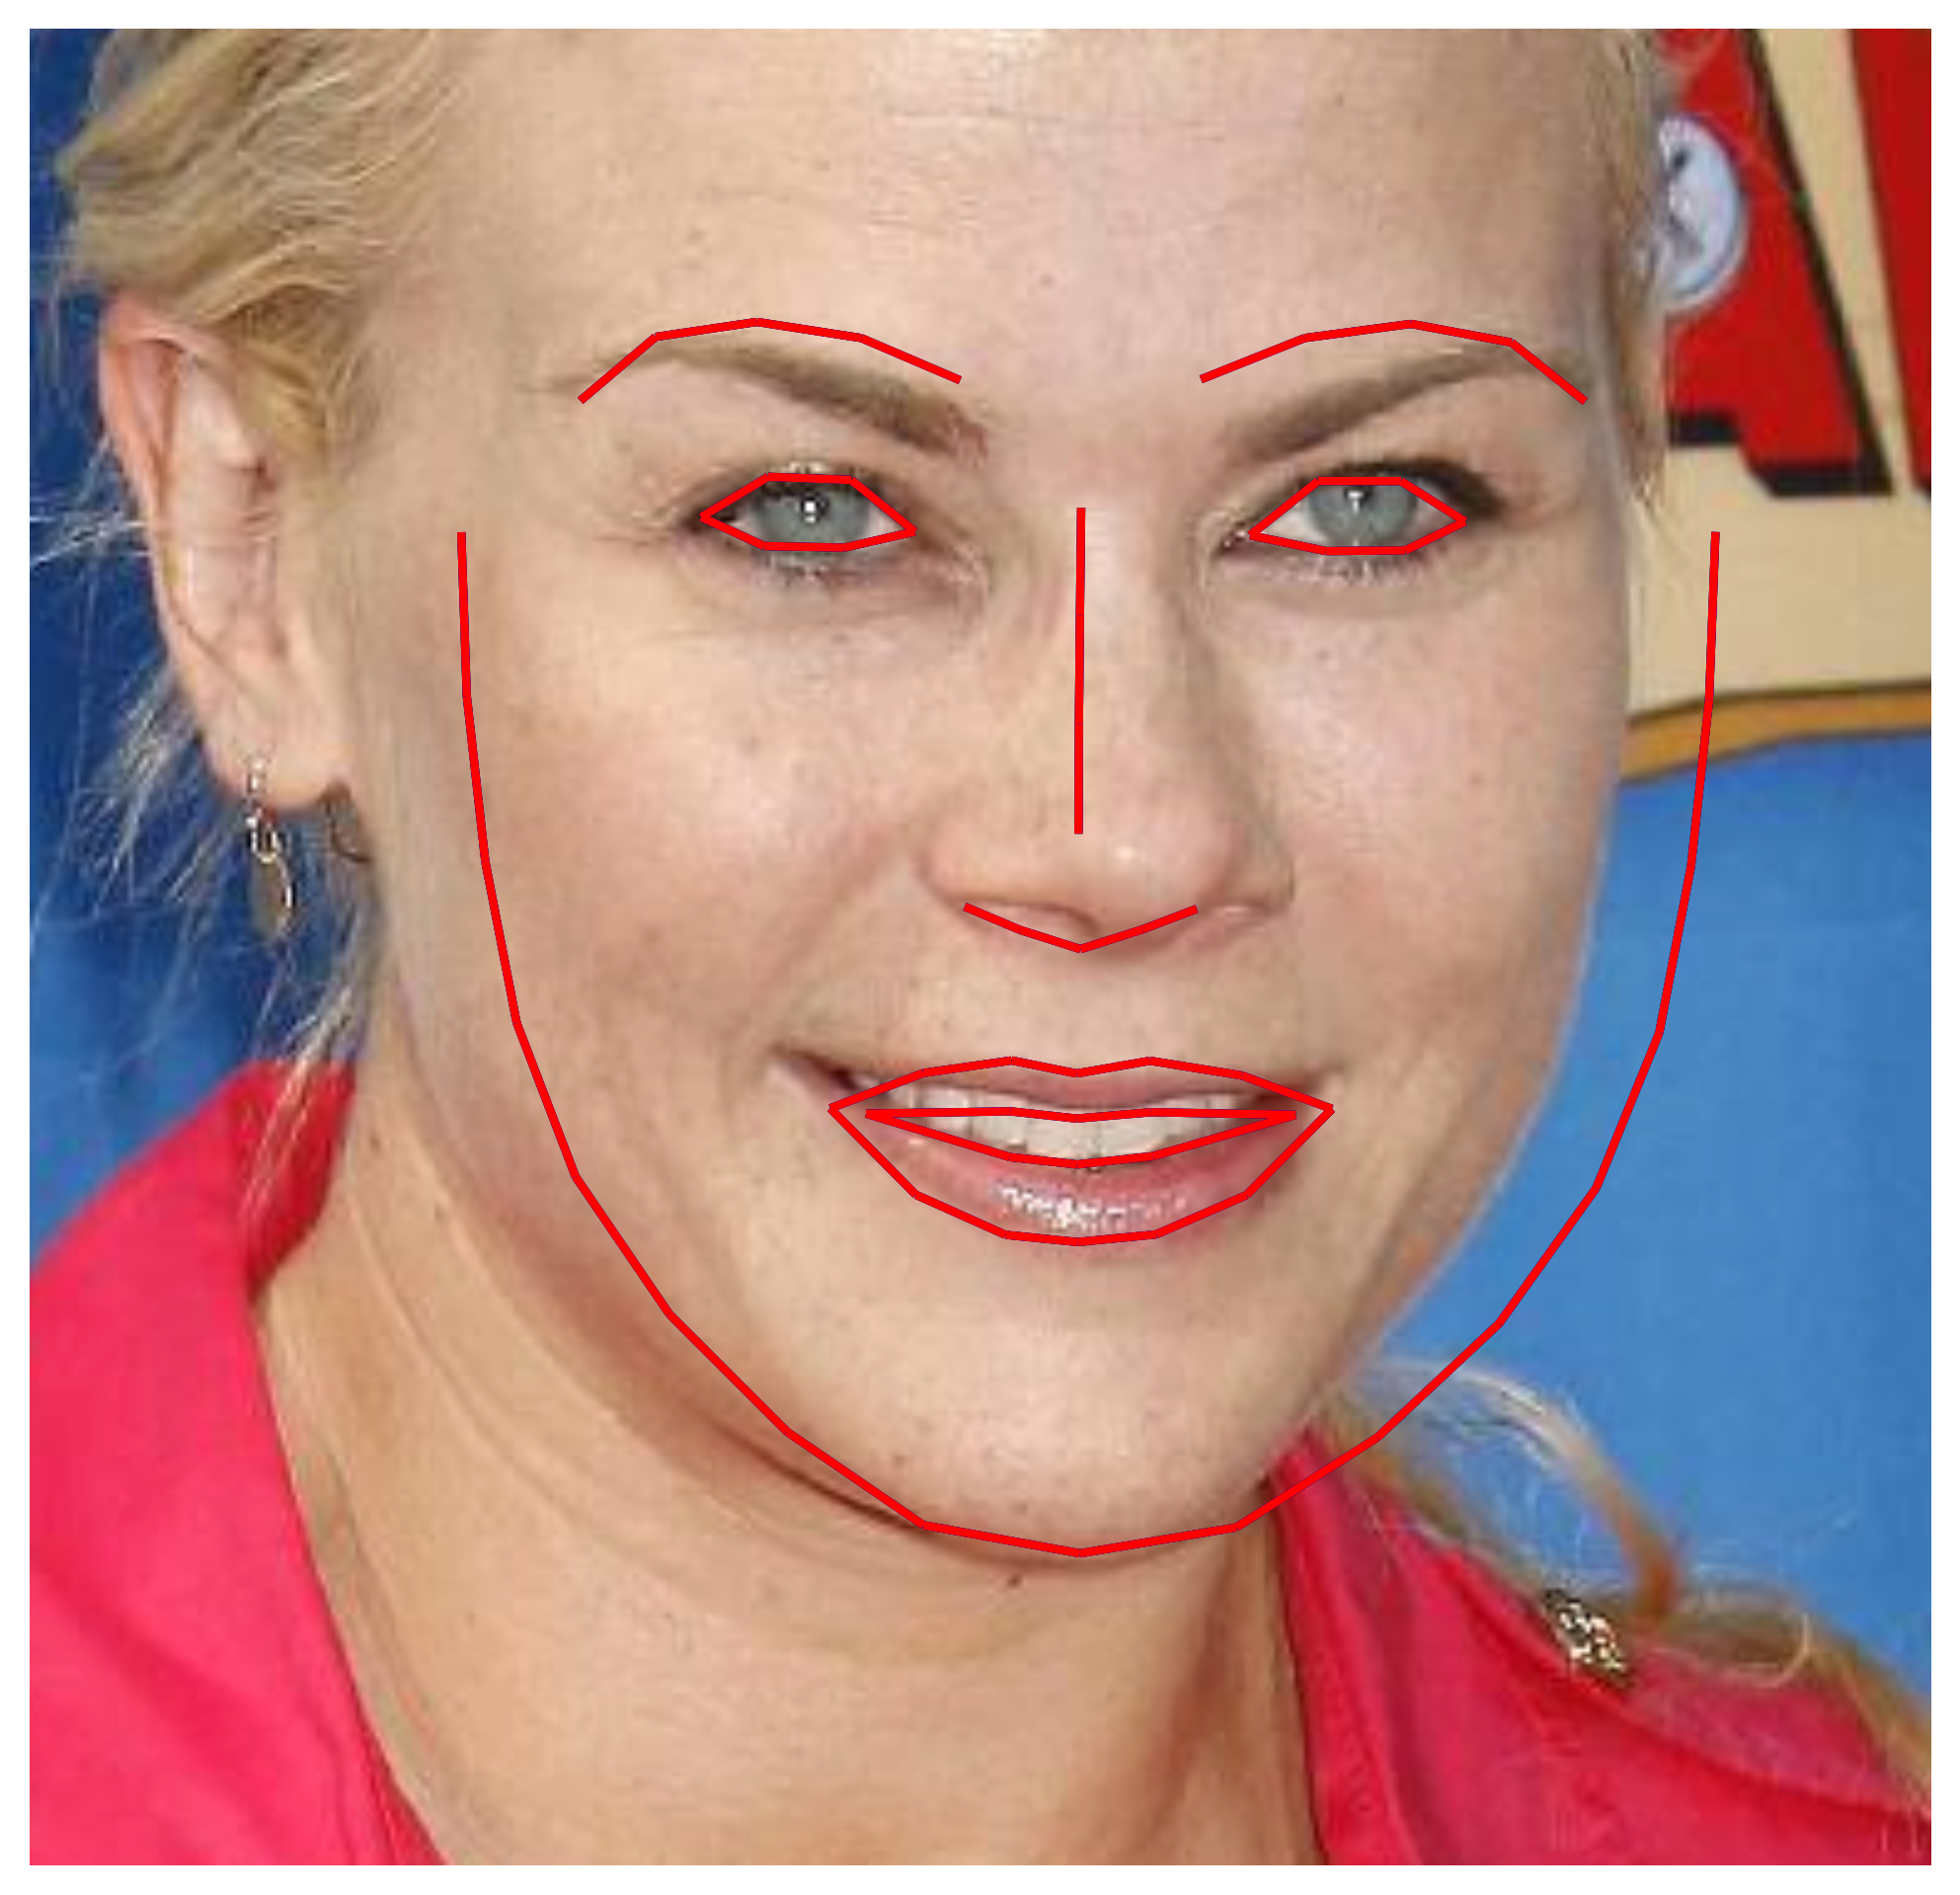
\includegraphics[width=\textwidth]{figures/ini_0.png}
		\caption{$0\%$}
		\label{fig:ini_0}
	\end{subfigure}
	\begin{subfigure}{0.16\textwidth}
		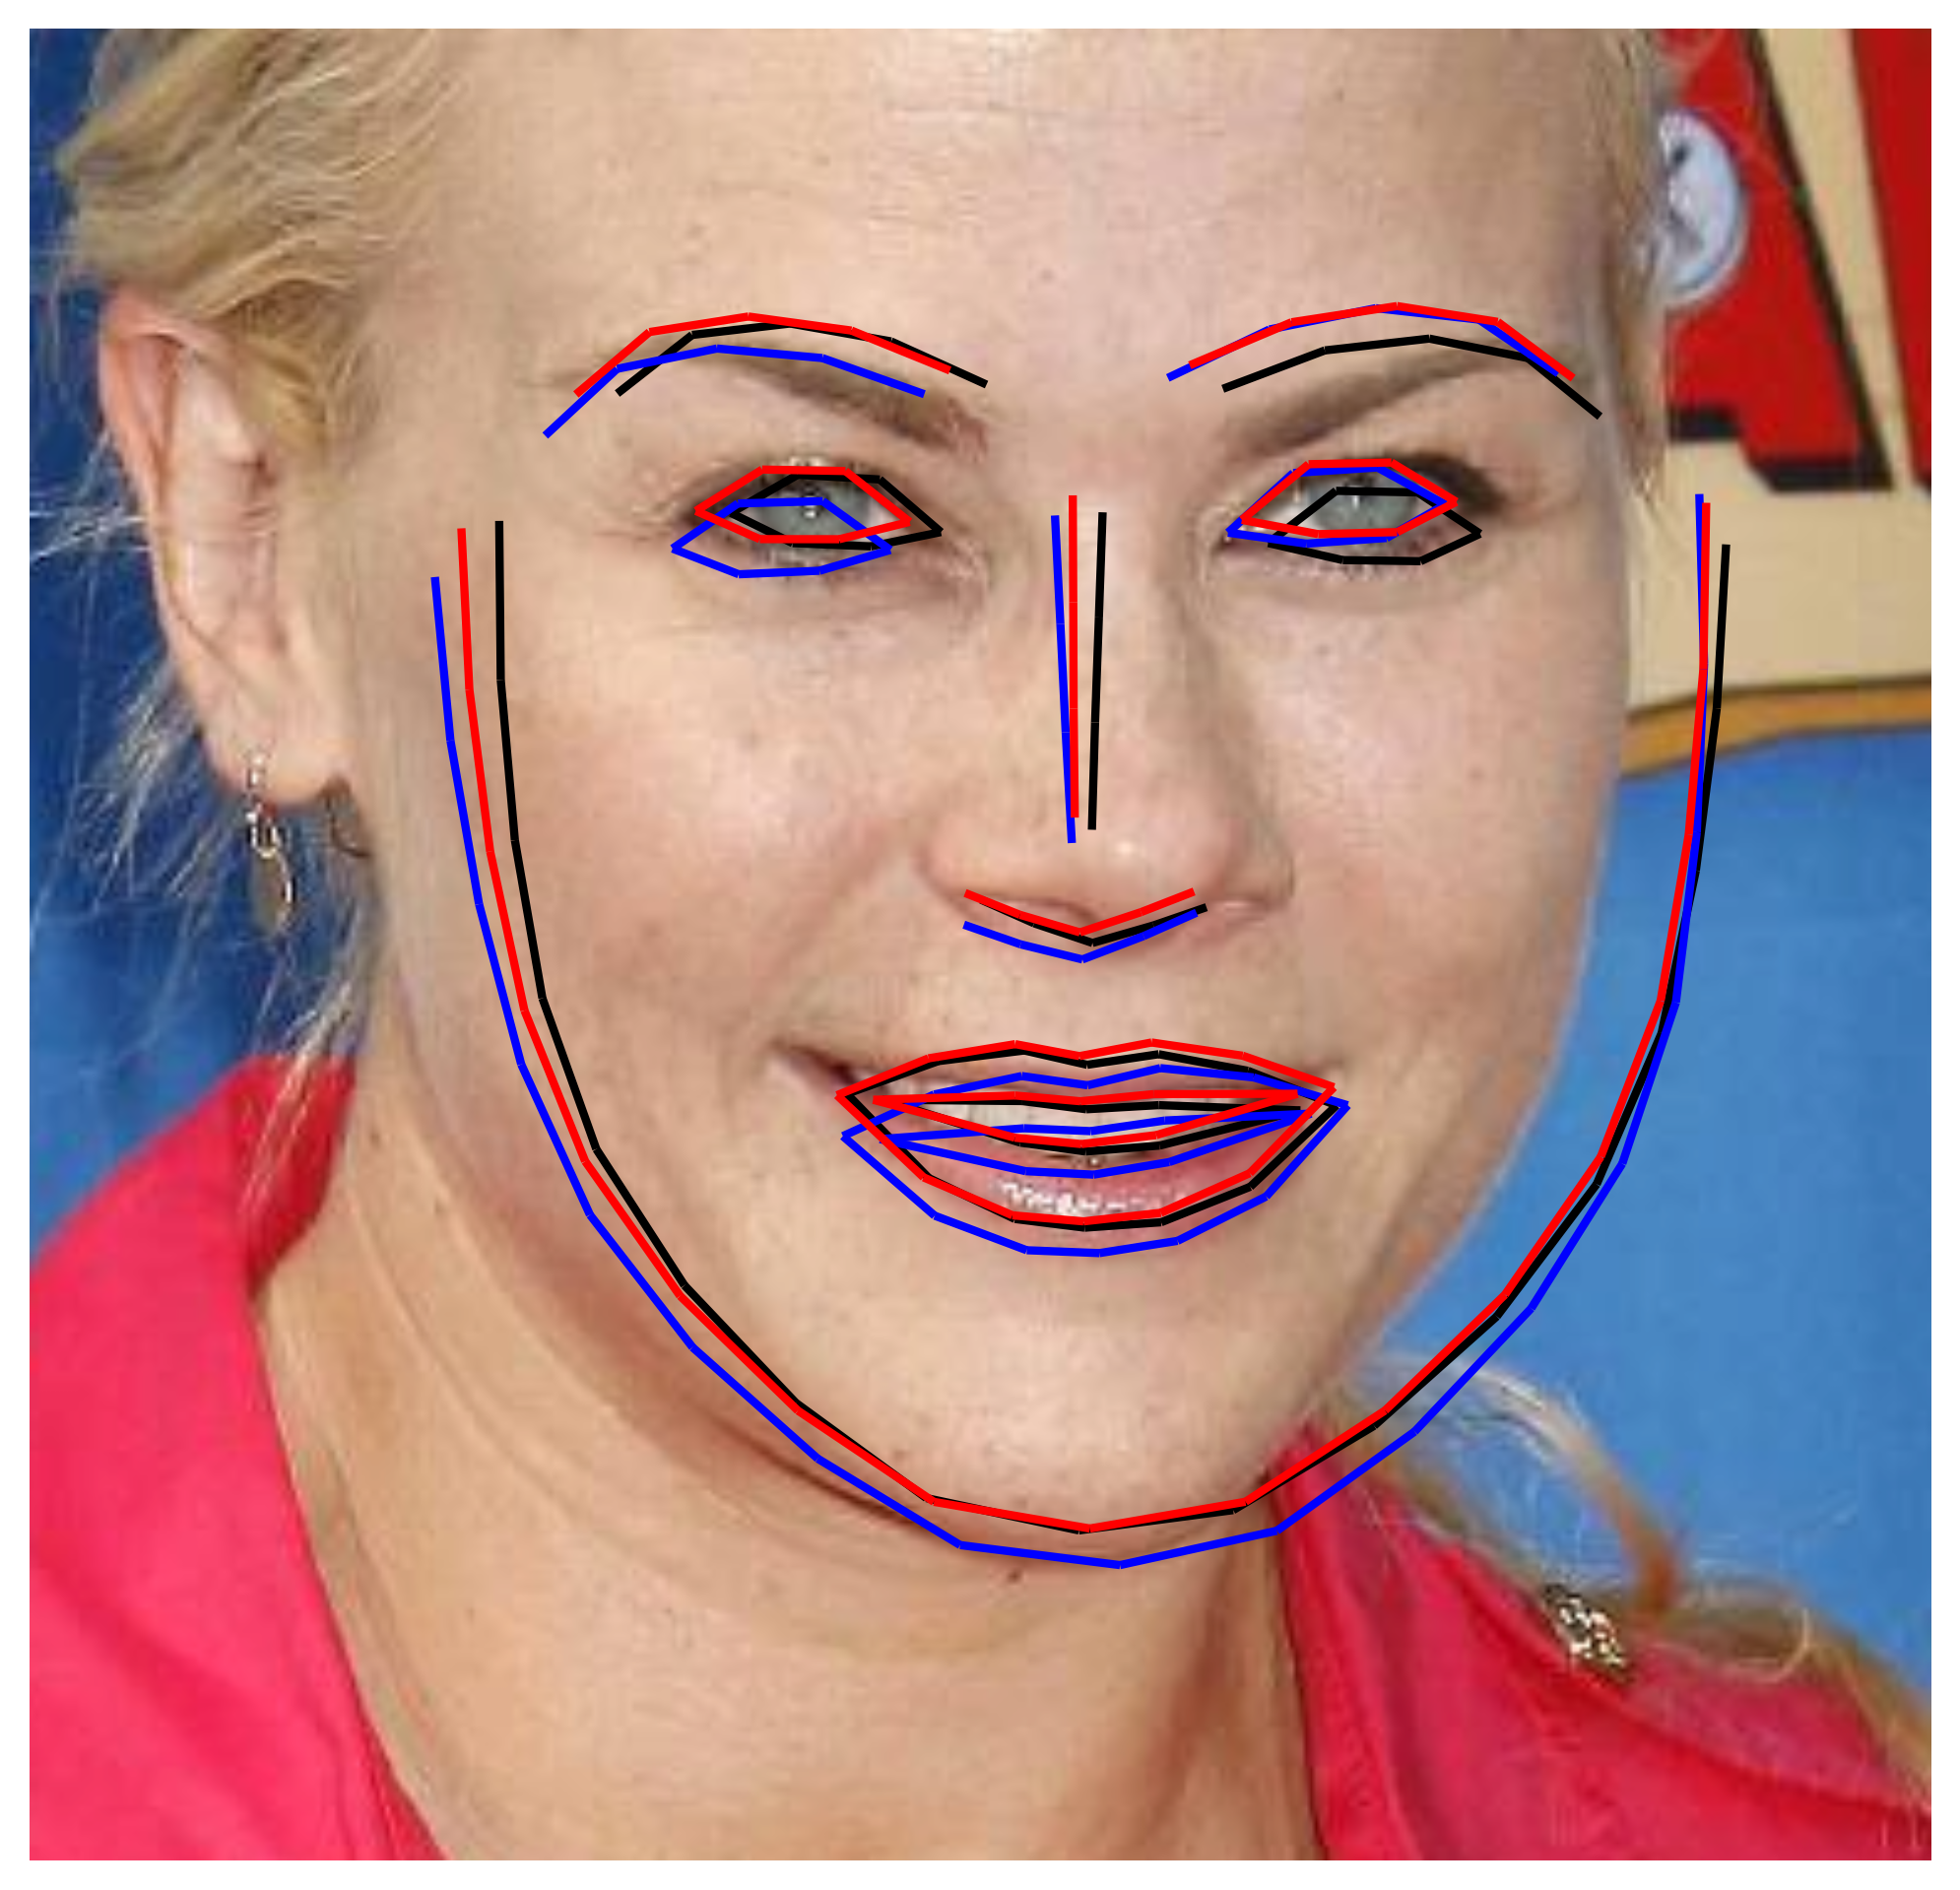
\includegraphics[width=\textwidth]{figures/ini_1.png}
		\caption{$2.5\%$}
		\label{fig:ini_1}
	\end{subfigure}
	\begin{subfigure}{0.16\textwidth}
		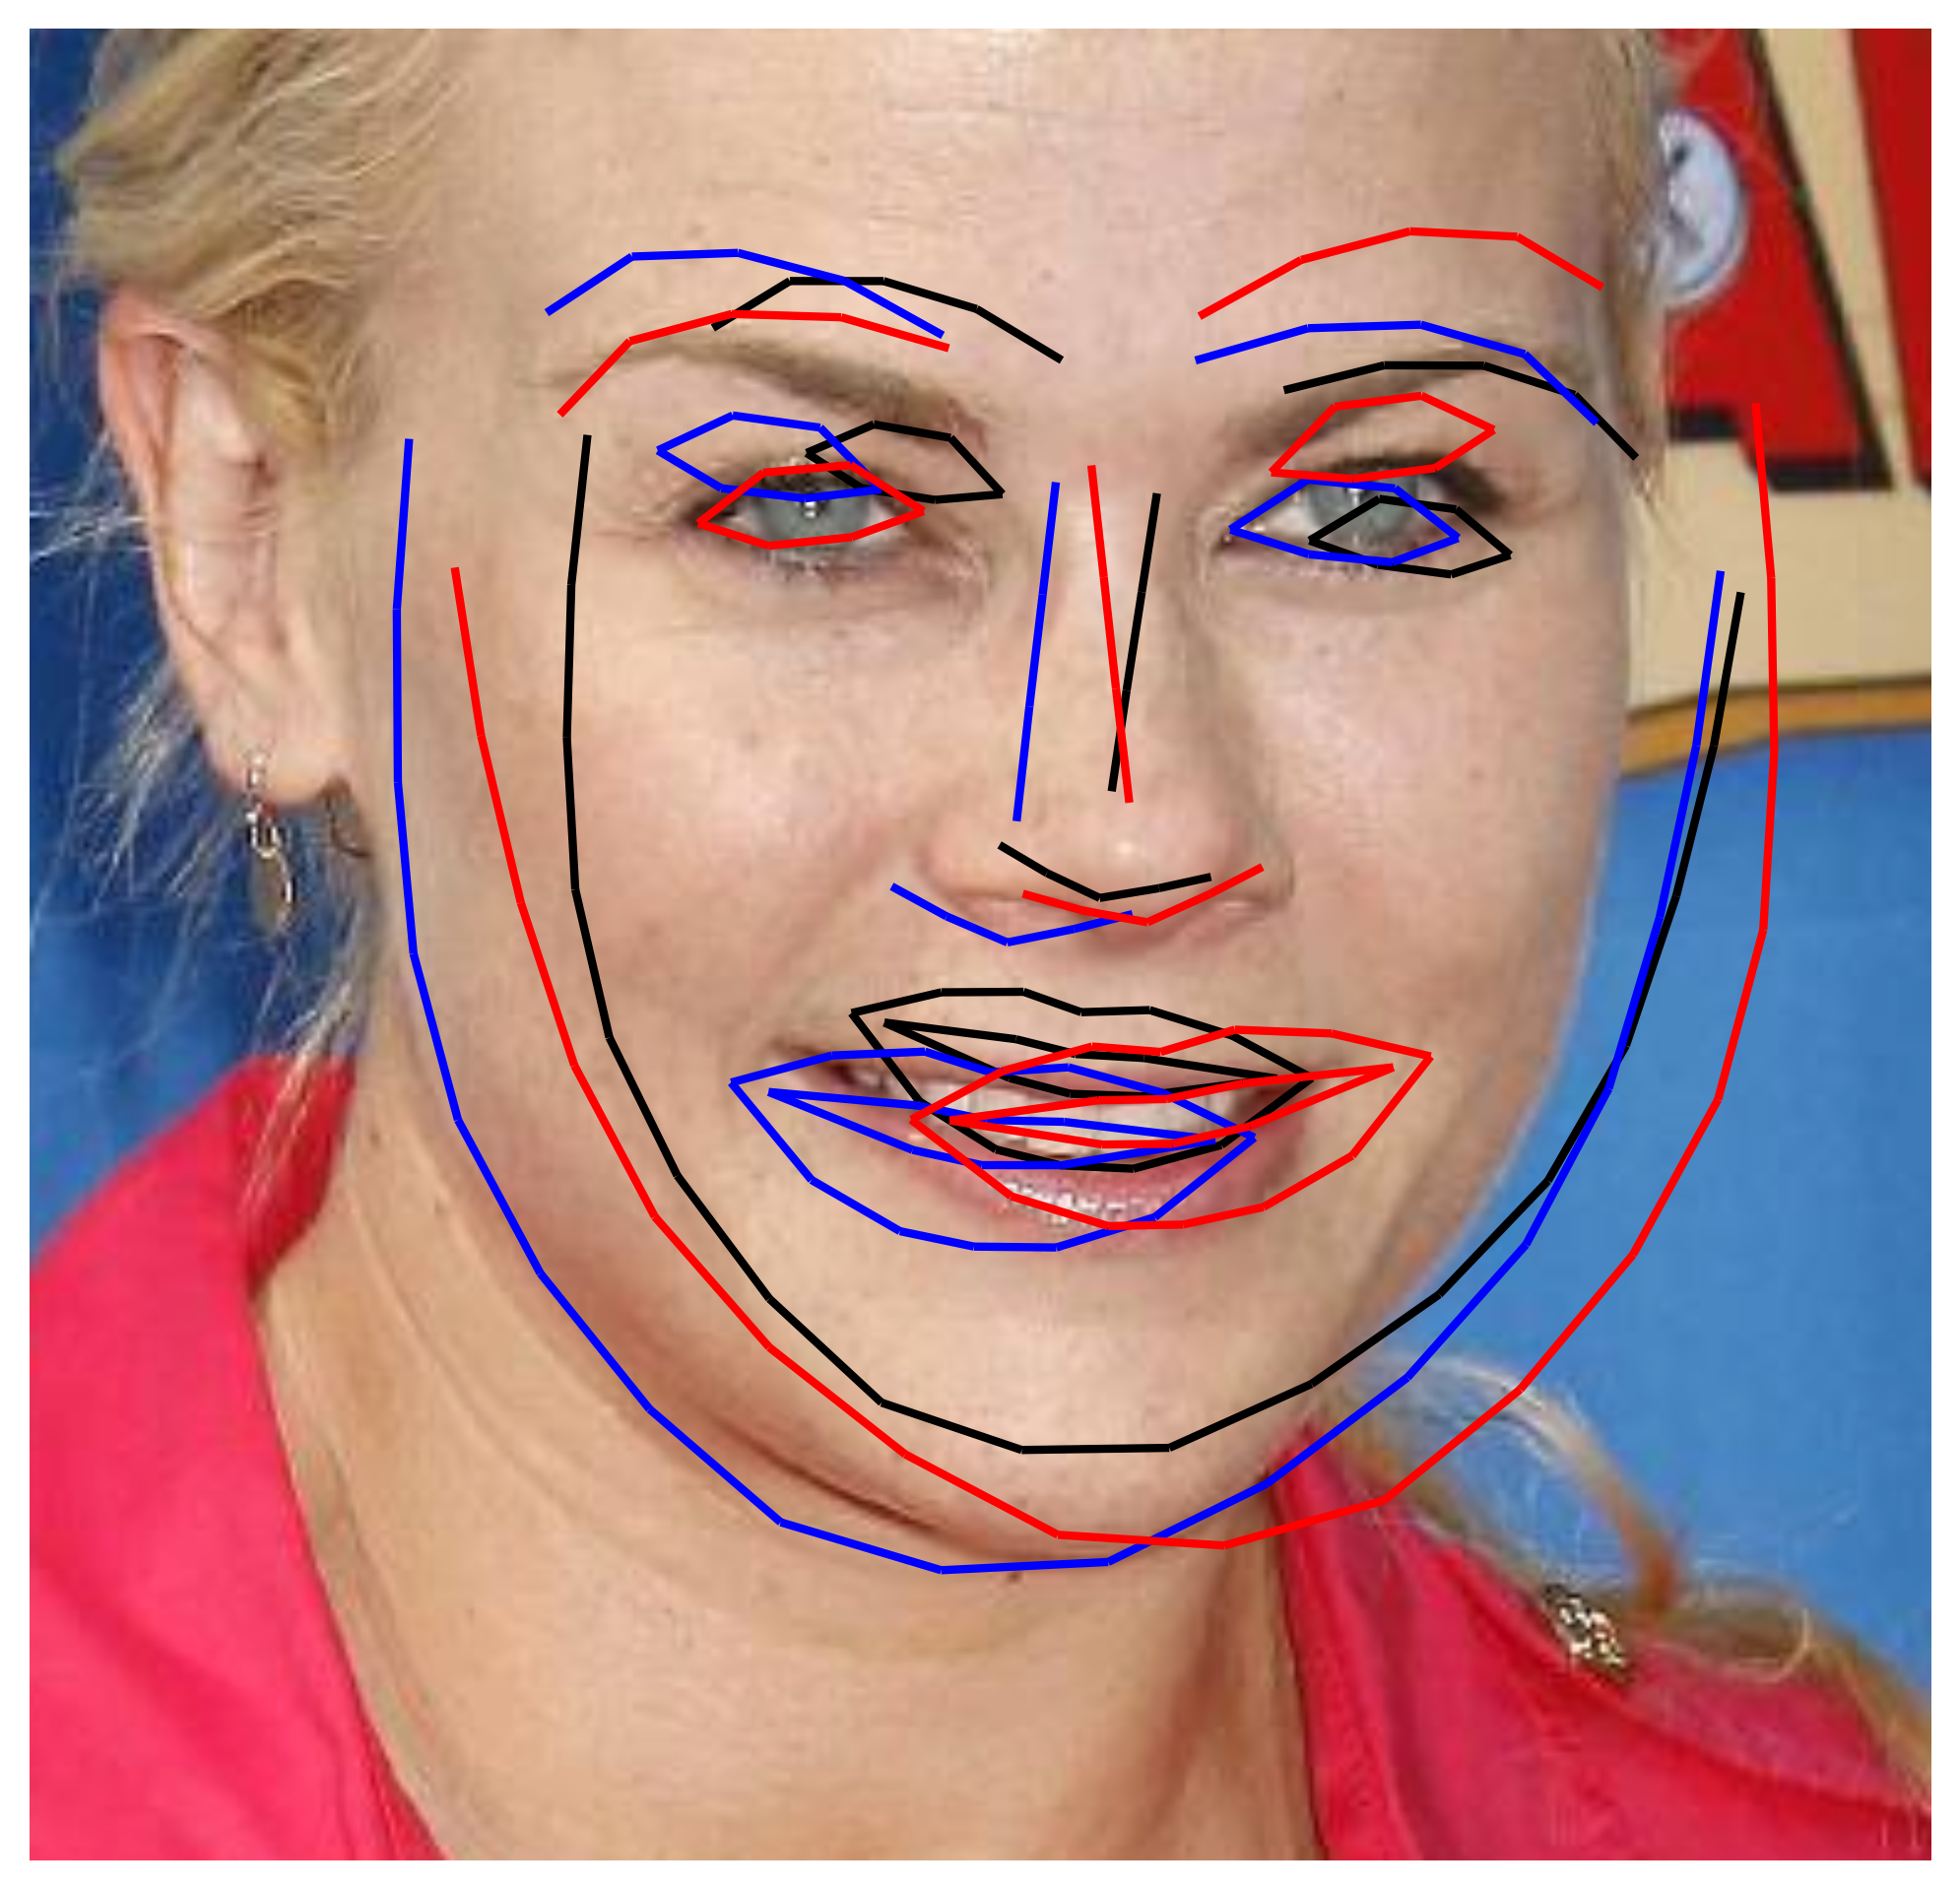
\includegraphics[width=\textwidth]{figures/ini_2.png}
		\caption{$5\%$}
		\label{fig:ini_2}
	\end{subfigure}
	\begin{subfigure}{0.16\textwidth}
		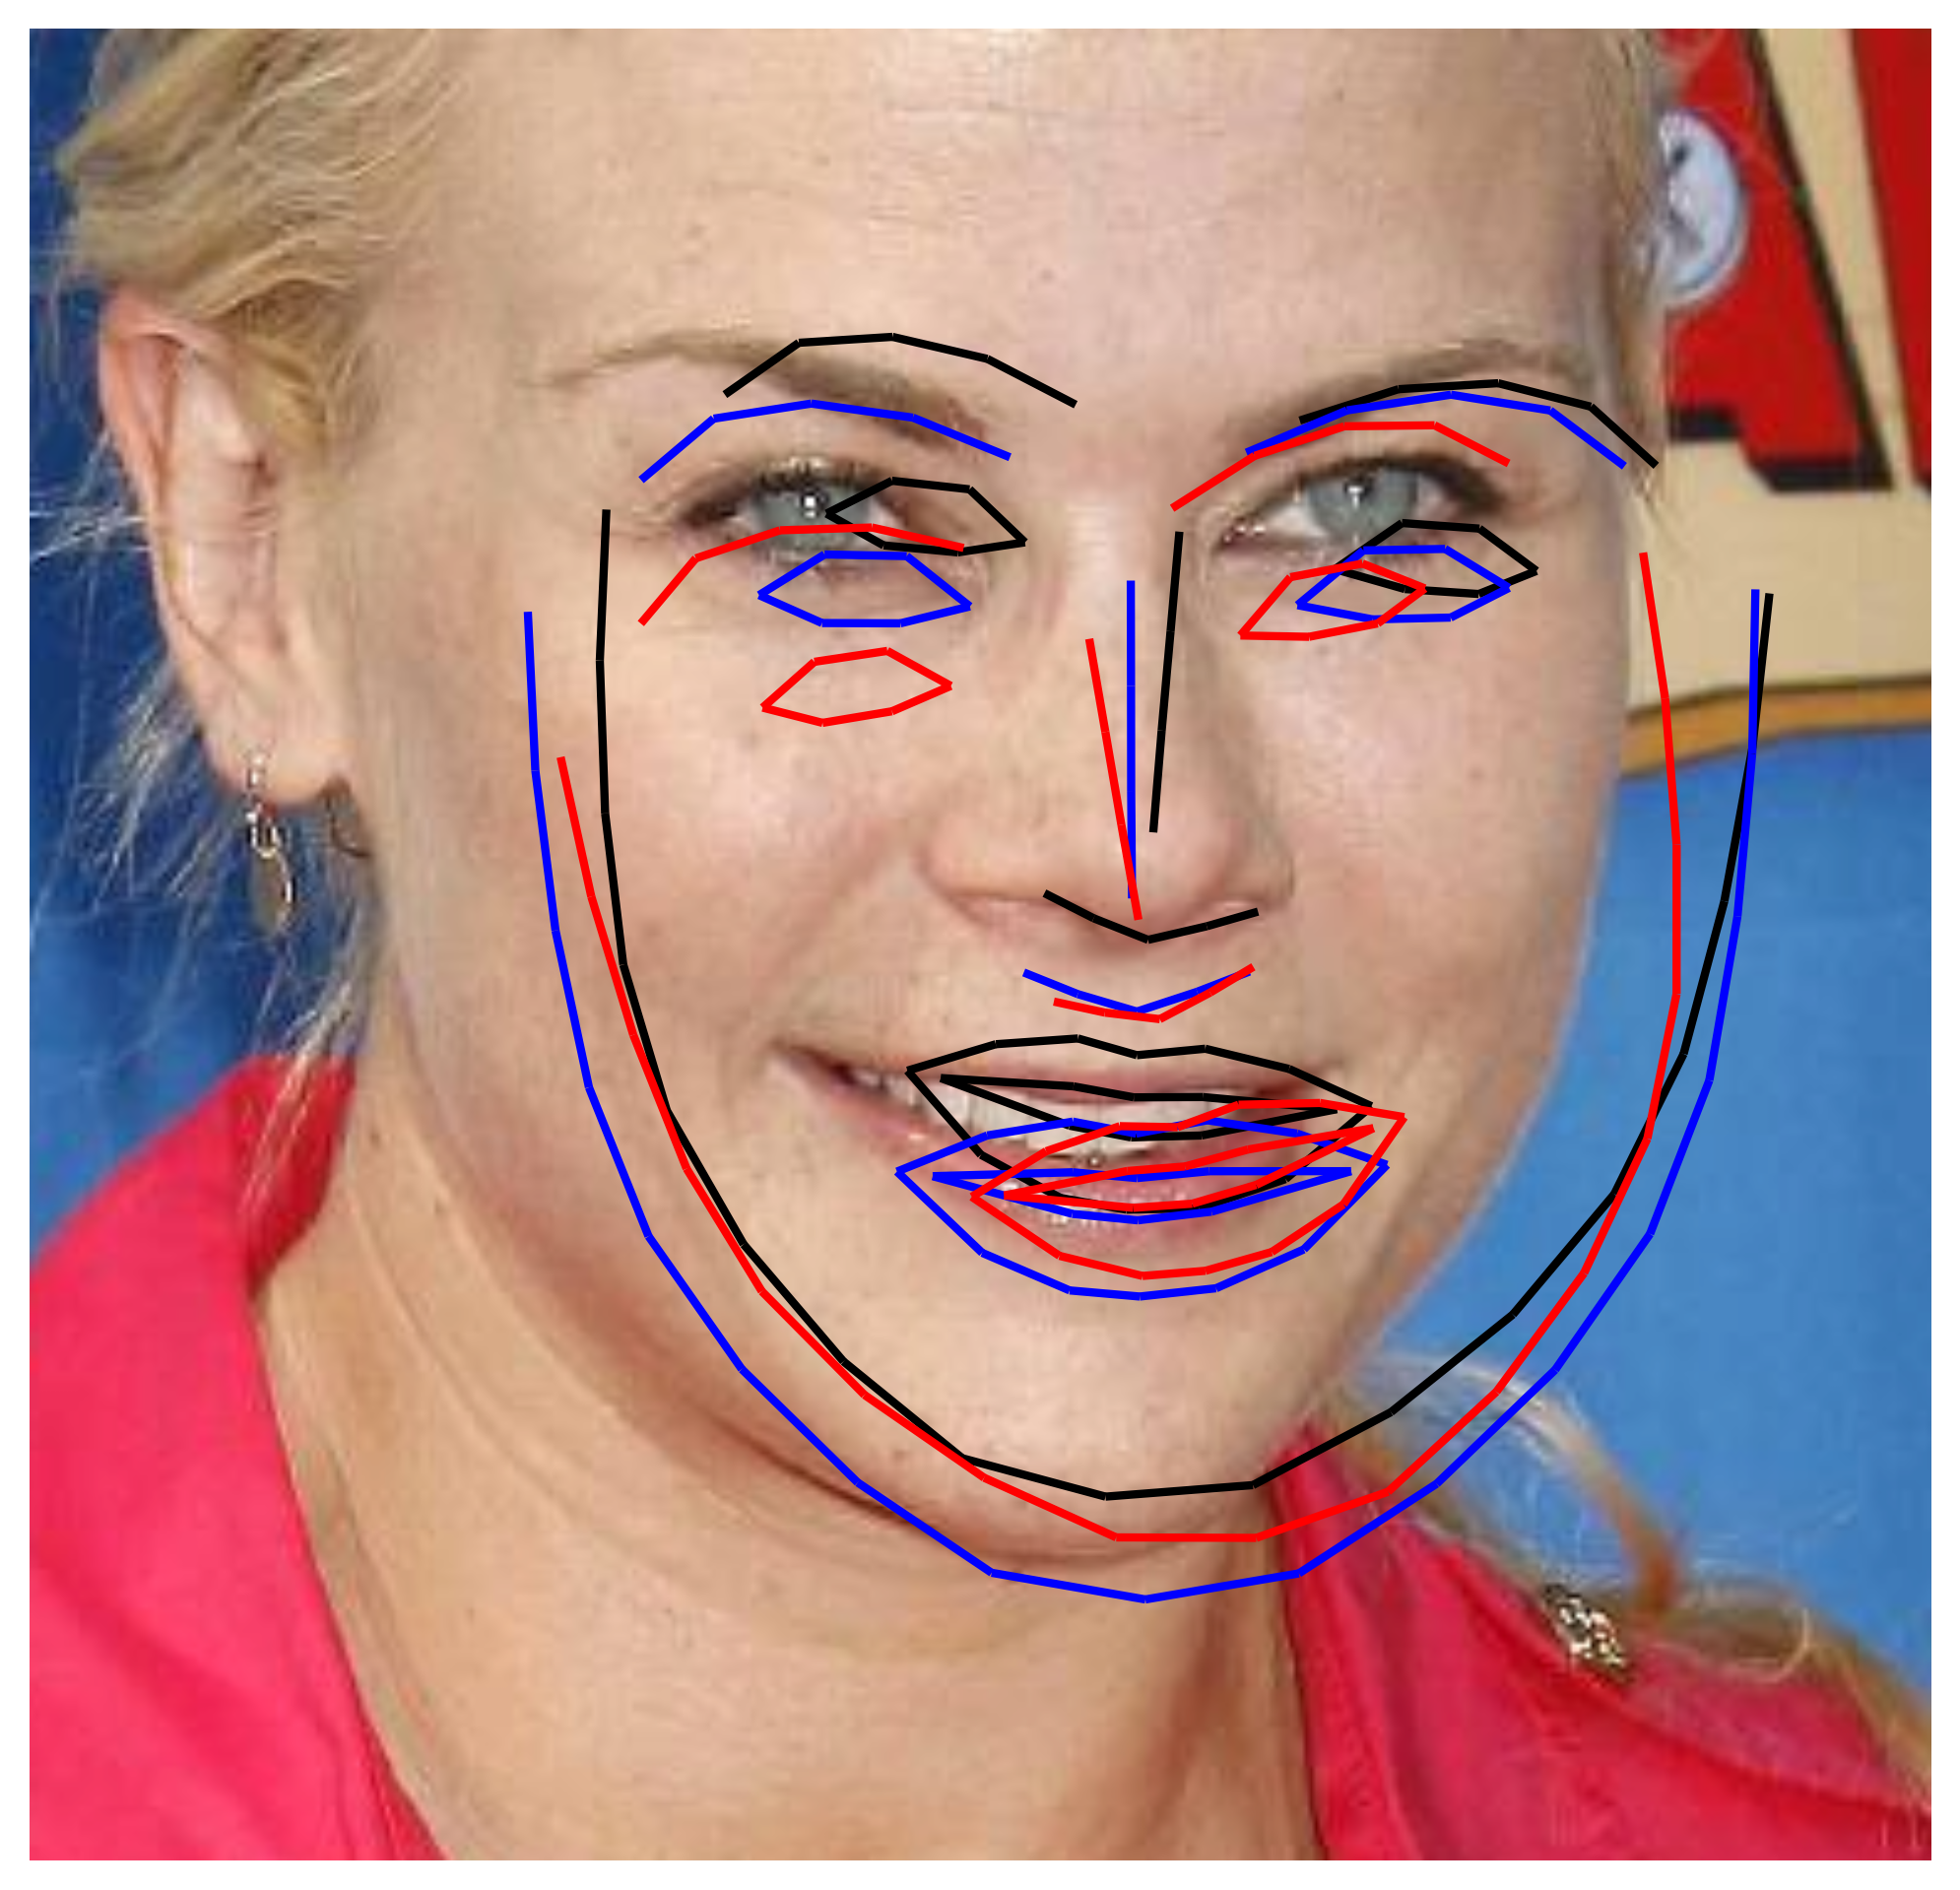
\includegraphics[width=\textwidth]{figures/ini_3.png}
		\caption{$7.5\%$}
		\label{fig:ini_3}
	\end{subfigure}
	\begin{subfigure}{0.16\textwidth}
		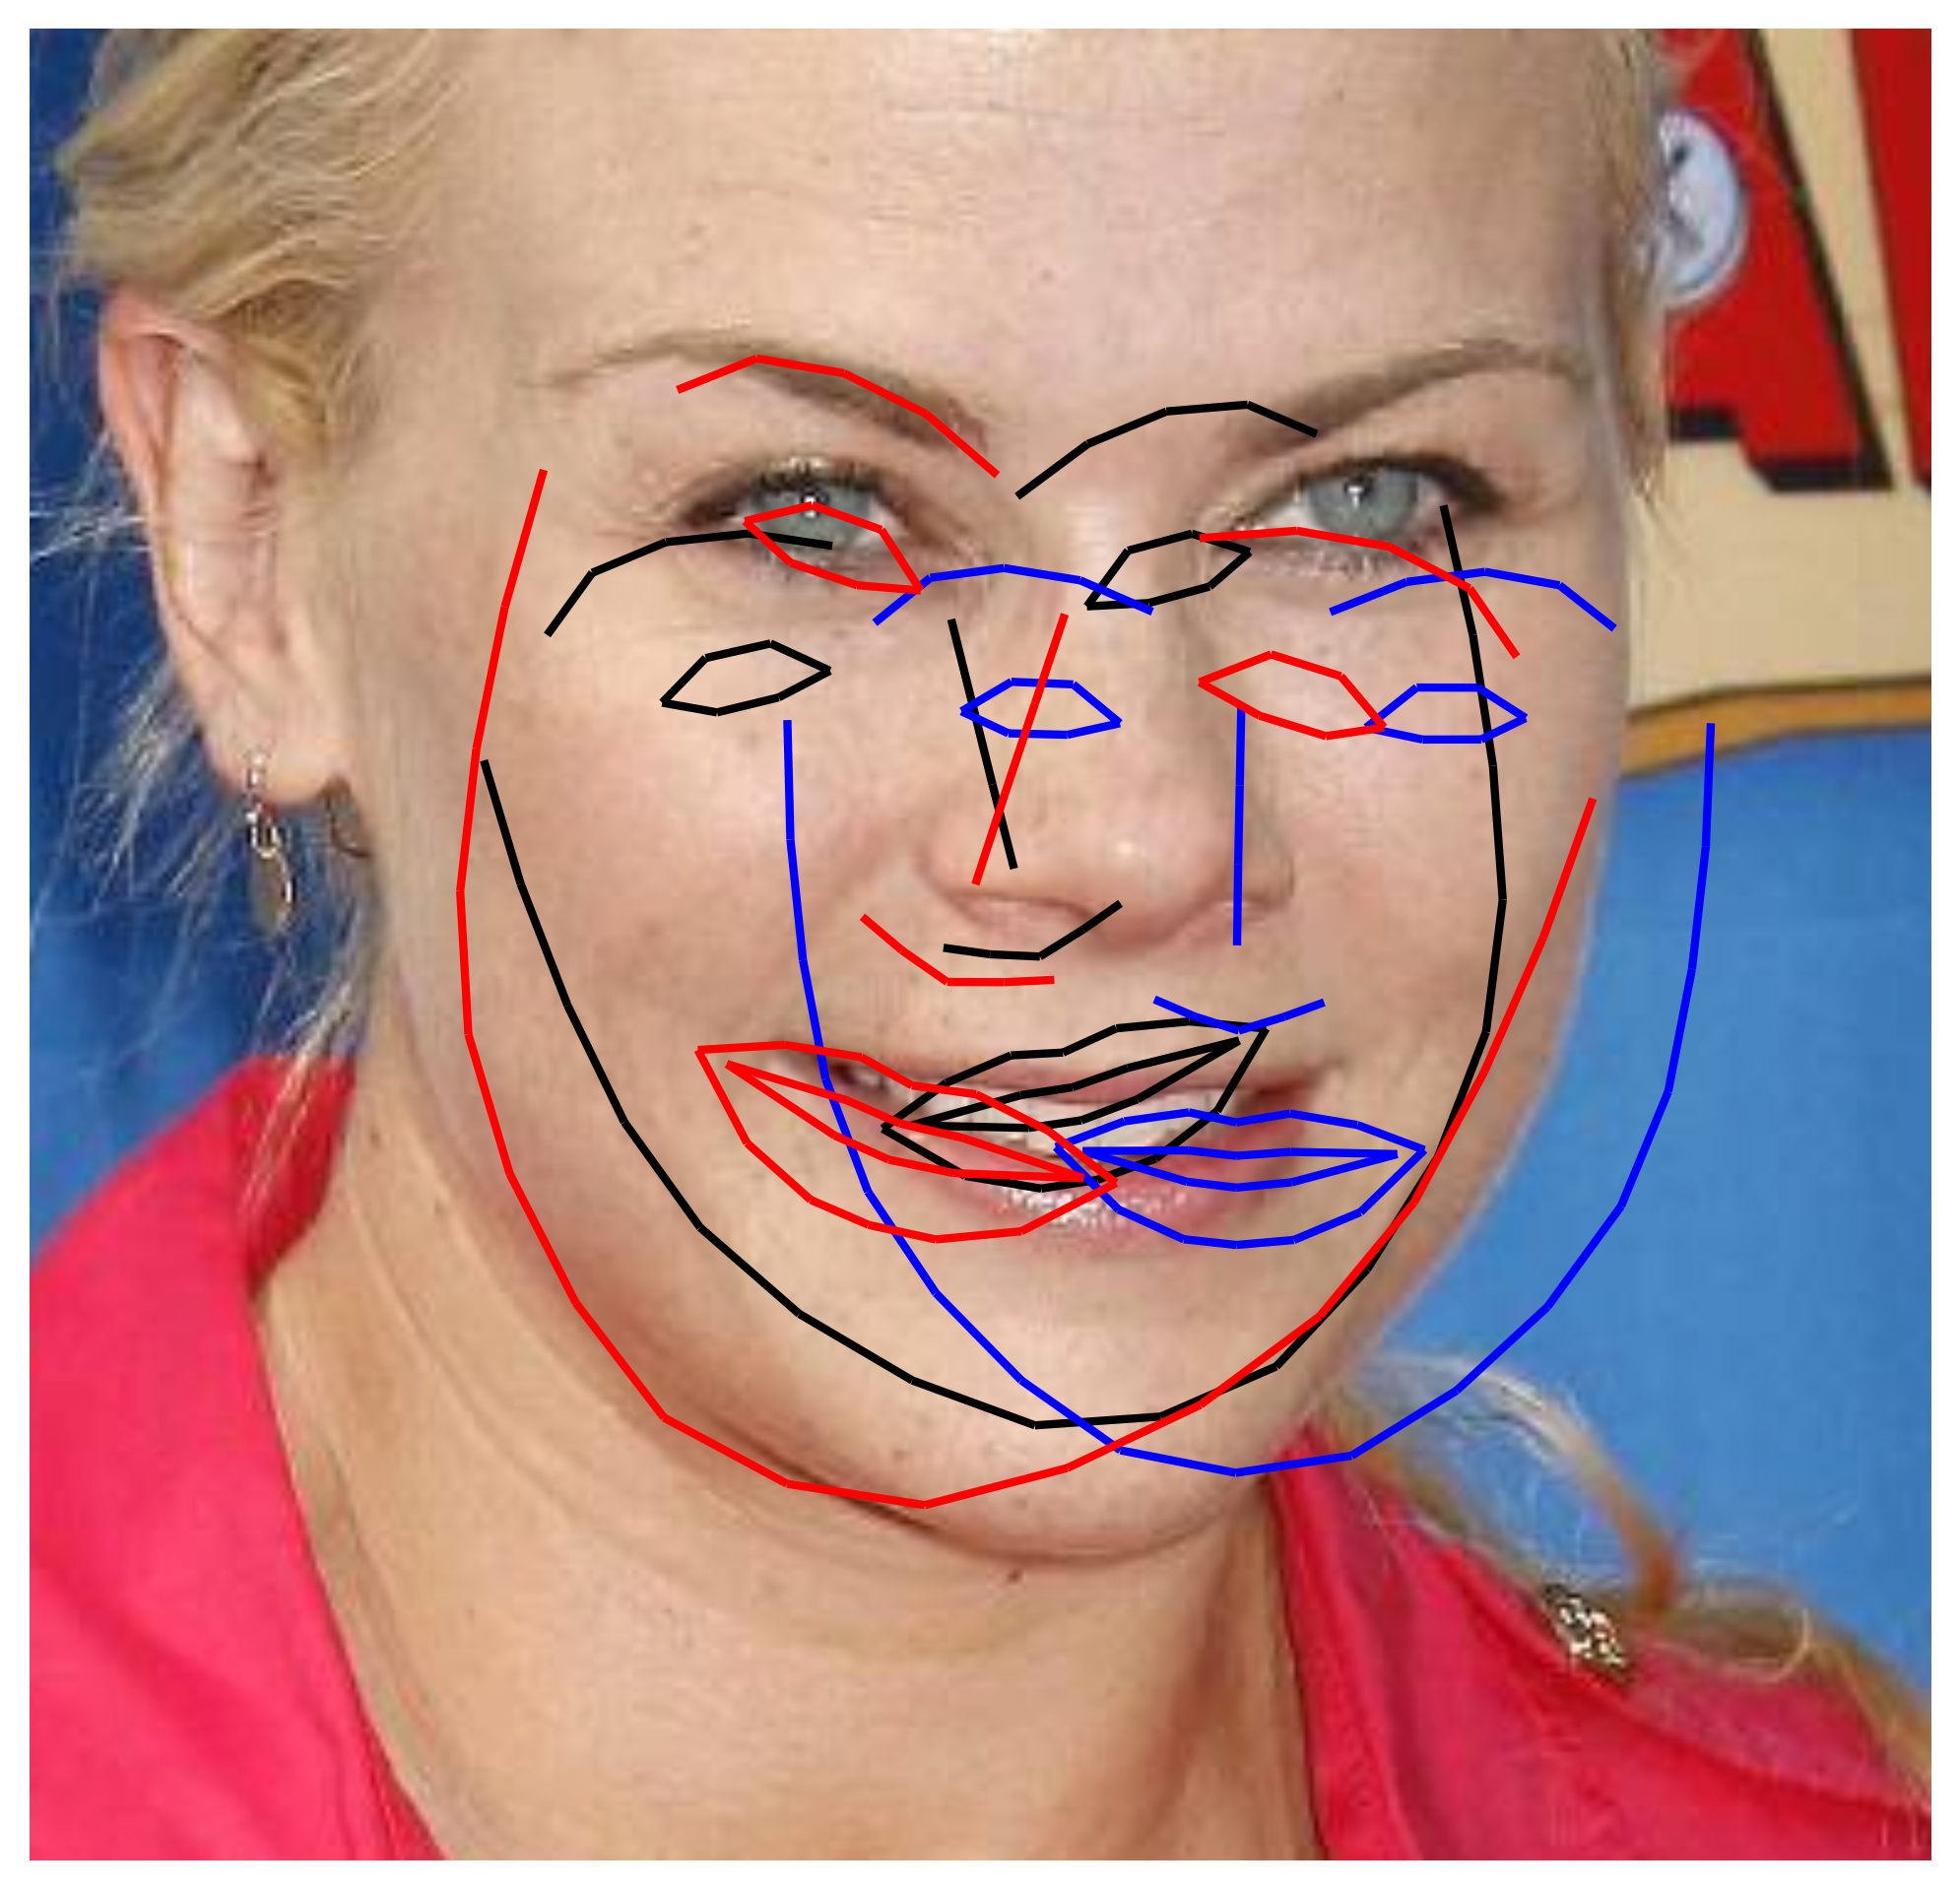
\includegraphics[width=\textwidth]{figures/ini_4.png}
		\caption{$10\%$}
		\label{fig:ini_4}
	\end{subfigure}
    \caption{Exemplar initializations obtained by varying the percentage of uniform noise added to the similarity parameters. Note that, increasing the percentage of noise produces more challenging initialization.}
    \label{fig:ini}
\end{figure*}

Finally, Kossaifi et al. derived the \emph{SSD Inverse Newton Schur} algorithm in \cite{Kossaifi2014}. This algorithm has a total complexity per iteration of $O(nmF + n^2m + 2n^2F + n^3)$ and was shown to slightly underperform its equivalent Gauss-Newton counterpart.

The remaining SSD algorithms derived in Section \ref{sec:fitting}, i.e.:
\begin{itemize}
\item \emph{SSD Inverse Wiberg}
\item \emph{SSD Forward Gauss-Newton Alternated}
\item \emph{SSD Forward Newton Schur}
\item \emph{SSD Forward Newton Alternated}
\item \emph{SSD Forward Wiberg}
\item \emph{SSD Asymmetric Gauss-Newton Schur}
\item \emph{SSD Asymmetric Gauss-Newton Alternated}
\item \emph{SSD Asymmetric Newton Schur}
\item \emph{SSD Asymmetric Newton Alternated}
\item \emph{SSD Asymmetric Wiberg}
\item \emph{SSD Bidirectional Gauss-Newton Schur}
\item \emph{SSD Bidirectional Gauss-Newton Alternated}
\item \emph{SSD Bidirectional Newton Schur}
\item \emph{SSD Bidirectional Newton Alternated}
\item \emph{SSD Bidirectional Wiberg}
\end{itemize}
have never been published before and are also a key contribution of the presented work.

\section{Experiments}
\label{sec:experiment}

In this section we analyse the performance of all CGD algorithms derived in Section \ref{sec:fitting} on the specific problem of non-rigid face alignment in-the-wild. We start by quantifying the fitting accuracy and convergence properties of each algorithm. Then we

All algorithms were tested using the same AAM which was built using $\sim800$  training images of the Labelled Face Parts in the Wild (LFPW) \cite{Belhumeur2011} and $\sim2000$ Helen \cite{Le2012} databases.

All algorithms are implemented using a coarse to fine optimization strategy using a gaussian pyramid with $2$ levels (face images are normalized to a \emph{face size}\footnote{We use the definition of face size given in \cite{Zhu2012} i.e. the mean of height and width of the face.} of roughly $150$ pixels at the top level). Similar to \cite{Tzimiropoulos2014}, we use a modified version of the \emph{Dense} Scale Invariant Feature Transform (DSIFT) \cite{Lowe1999, Dalal2005} to define the image representation of the linear appearance models. In particular, each pixel is described using a reduced DSIFT representation with $8$ features using the public implementation provided by the authors of \cite{Vedaldi2008vlfeat}. In all experiments, we optimized over $7$ shape parameters ($4$ similarity transform and $3$ non-rigid shape prameters) at the first pyramid level and over $16$ shape parameters ($4$ similarity transform and $12$ non-rigid shape prameters) at the second one. The dimensionality of the both appearance models is kept to represent $75\%$ of the total variance. This results in $225$ and $280$ appearance parameters at the first and second piramid levels respectively.

In this paper, we treated all previous parameters as hyperparameters and we set their values experimentally after testing on a small hold out set of the training data. 

We initialize all algorithms in all experiments by perturbing the similarity transforms that align the shape model's mean shape (a frontal pose and neutral expression looking shape) to the ground truth shape of  each image. These transforms are perturbed by adding a particular amounts of uniformly distributed random noise to their scale, rotation and translation parameters. Exemplar initializations obtained by this procedure for different amounts of uniform noiseare shown in Figure \ref{fig:initializations}.


\subsection{Comparison on LFPW}

In this experiment, we report the fitting accuracy and convergence properties of each of the previous algorithms. In order to keep the information on each figure and table easily readible and interpretable the experiment by grouping al...


\subsubsection{SSD algorithms}


\subsubsection*{Gauss-Newton}

\begin{figure*}[h!]
	\centering
	\begin{subfigure}{0.48\textwidth}
	    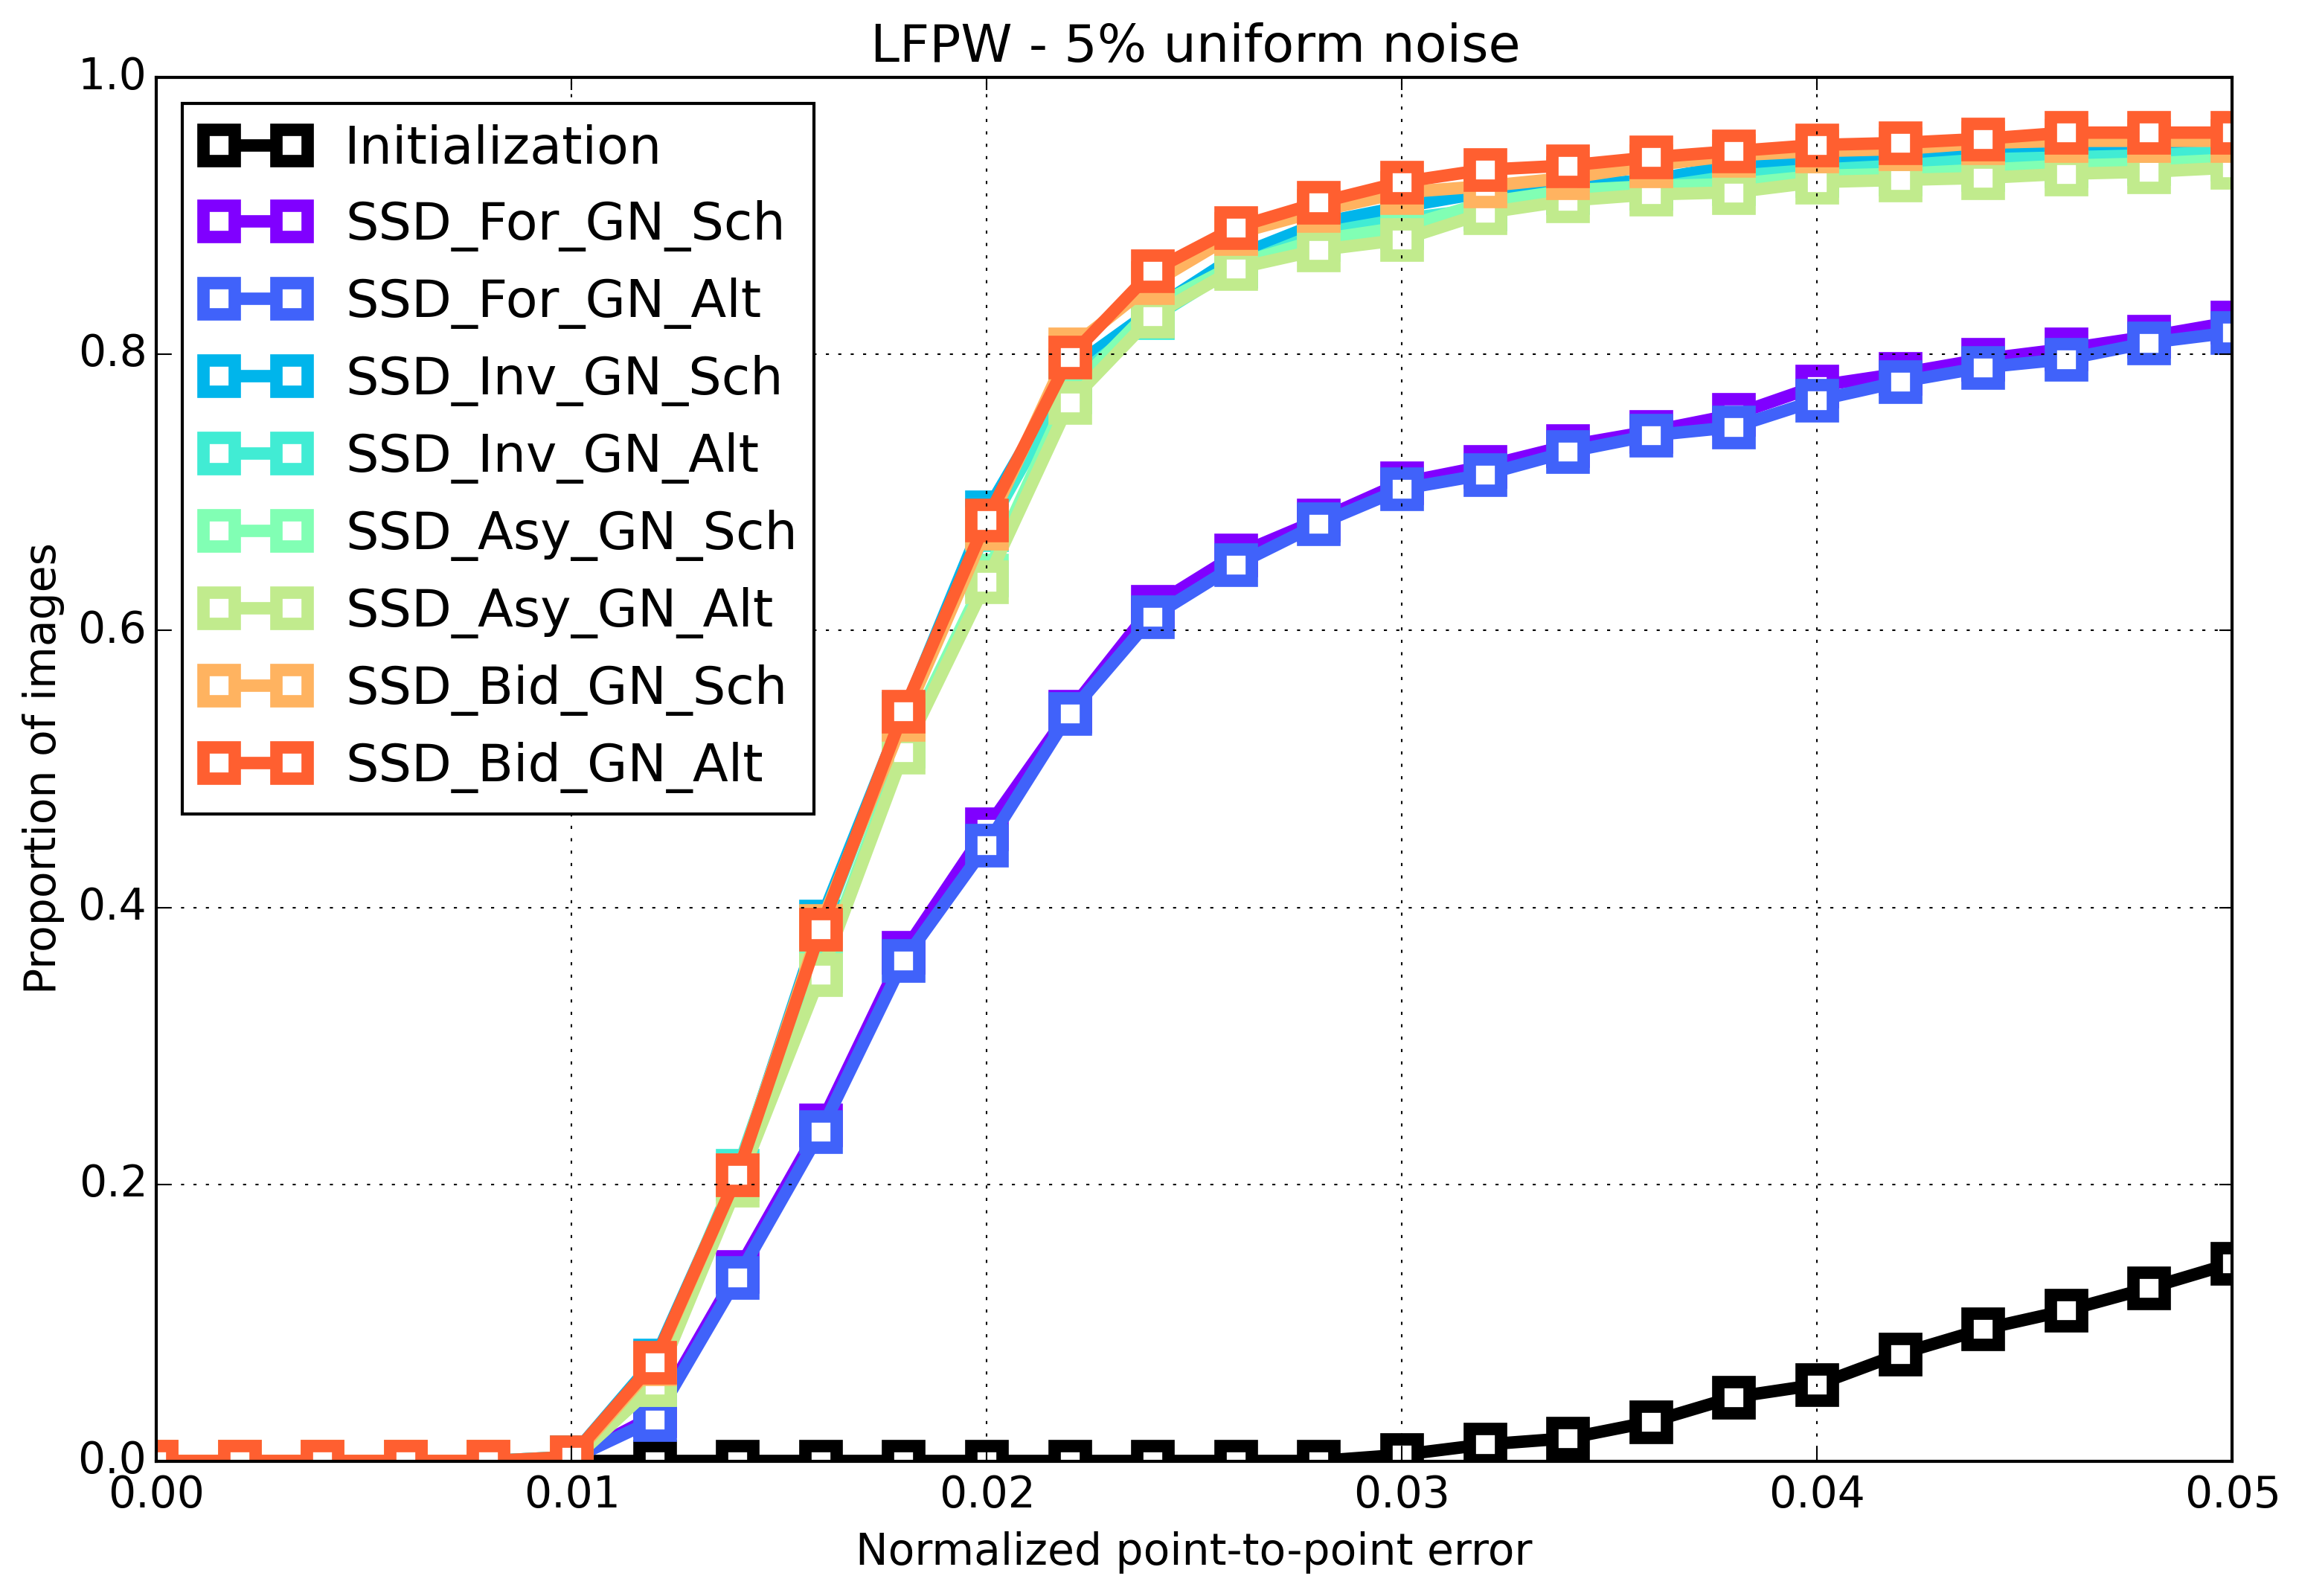
\includegraphics[width=\textwidth]{experiments/algorithms/ssd_gn/ced_ssd_gn_5.png}
	    \caption{Cumulative Error Distribution graph on the LFPW test dataset for all SSD Gauss-Newton algorithms initialized with $5\%$ uniform noise.}
	    \label{fig:ced_ssd_gn_5}
	\end{subfigure}
	\hfill
	\begin{subfigure}{0.48\textwidth}
	    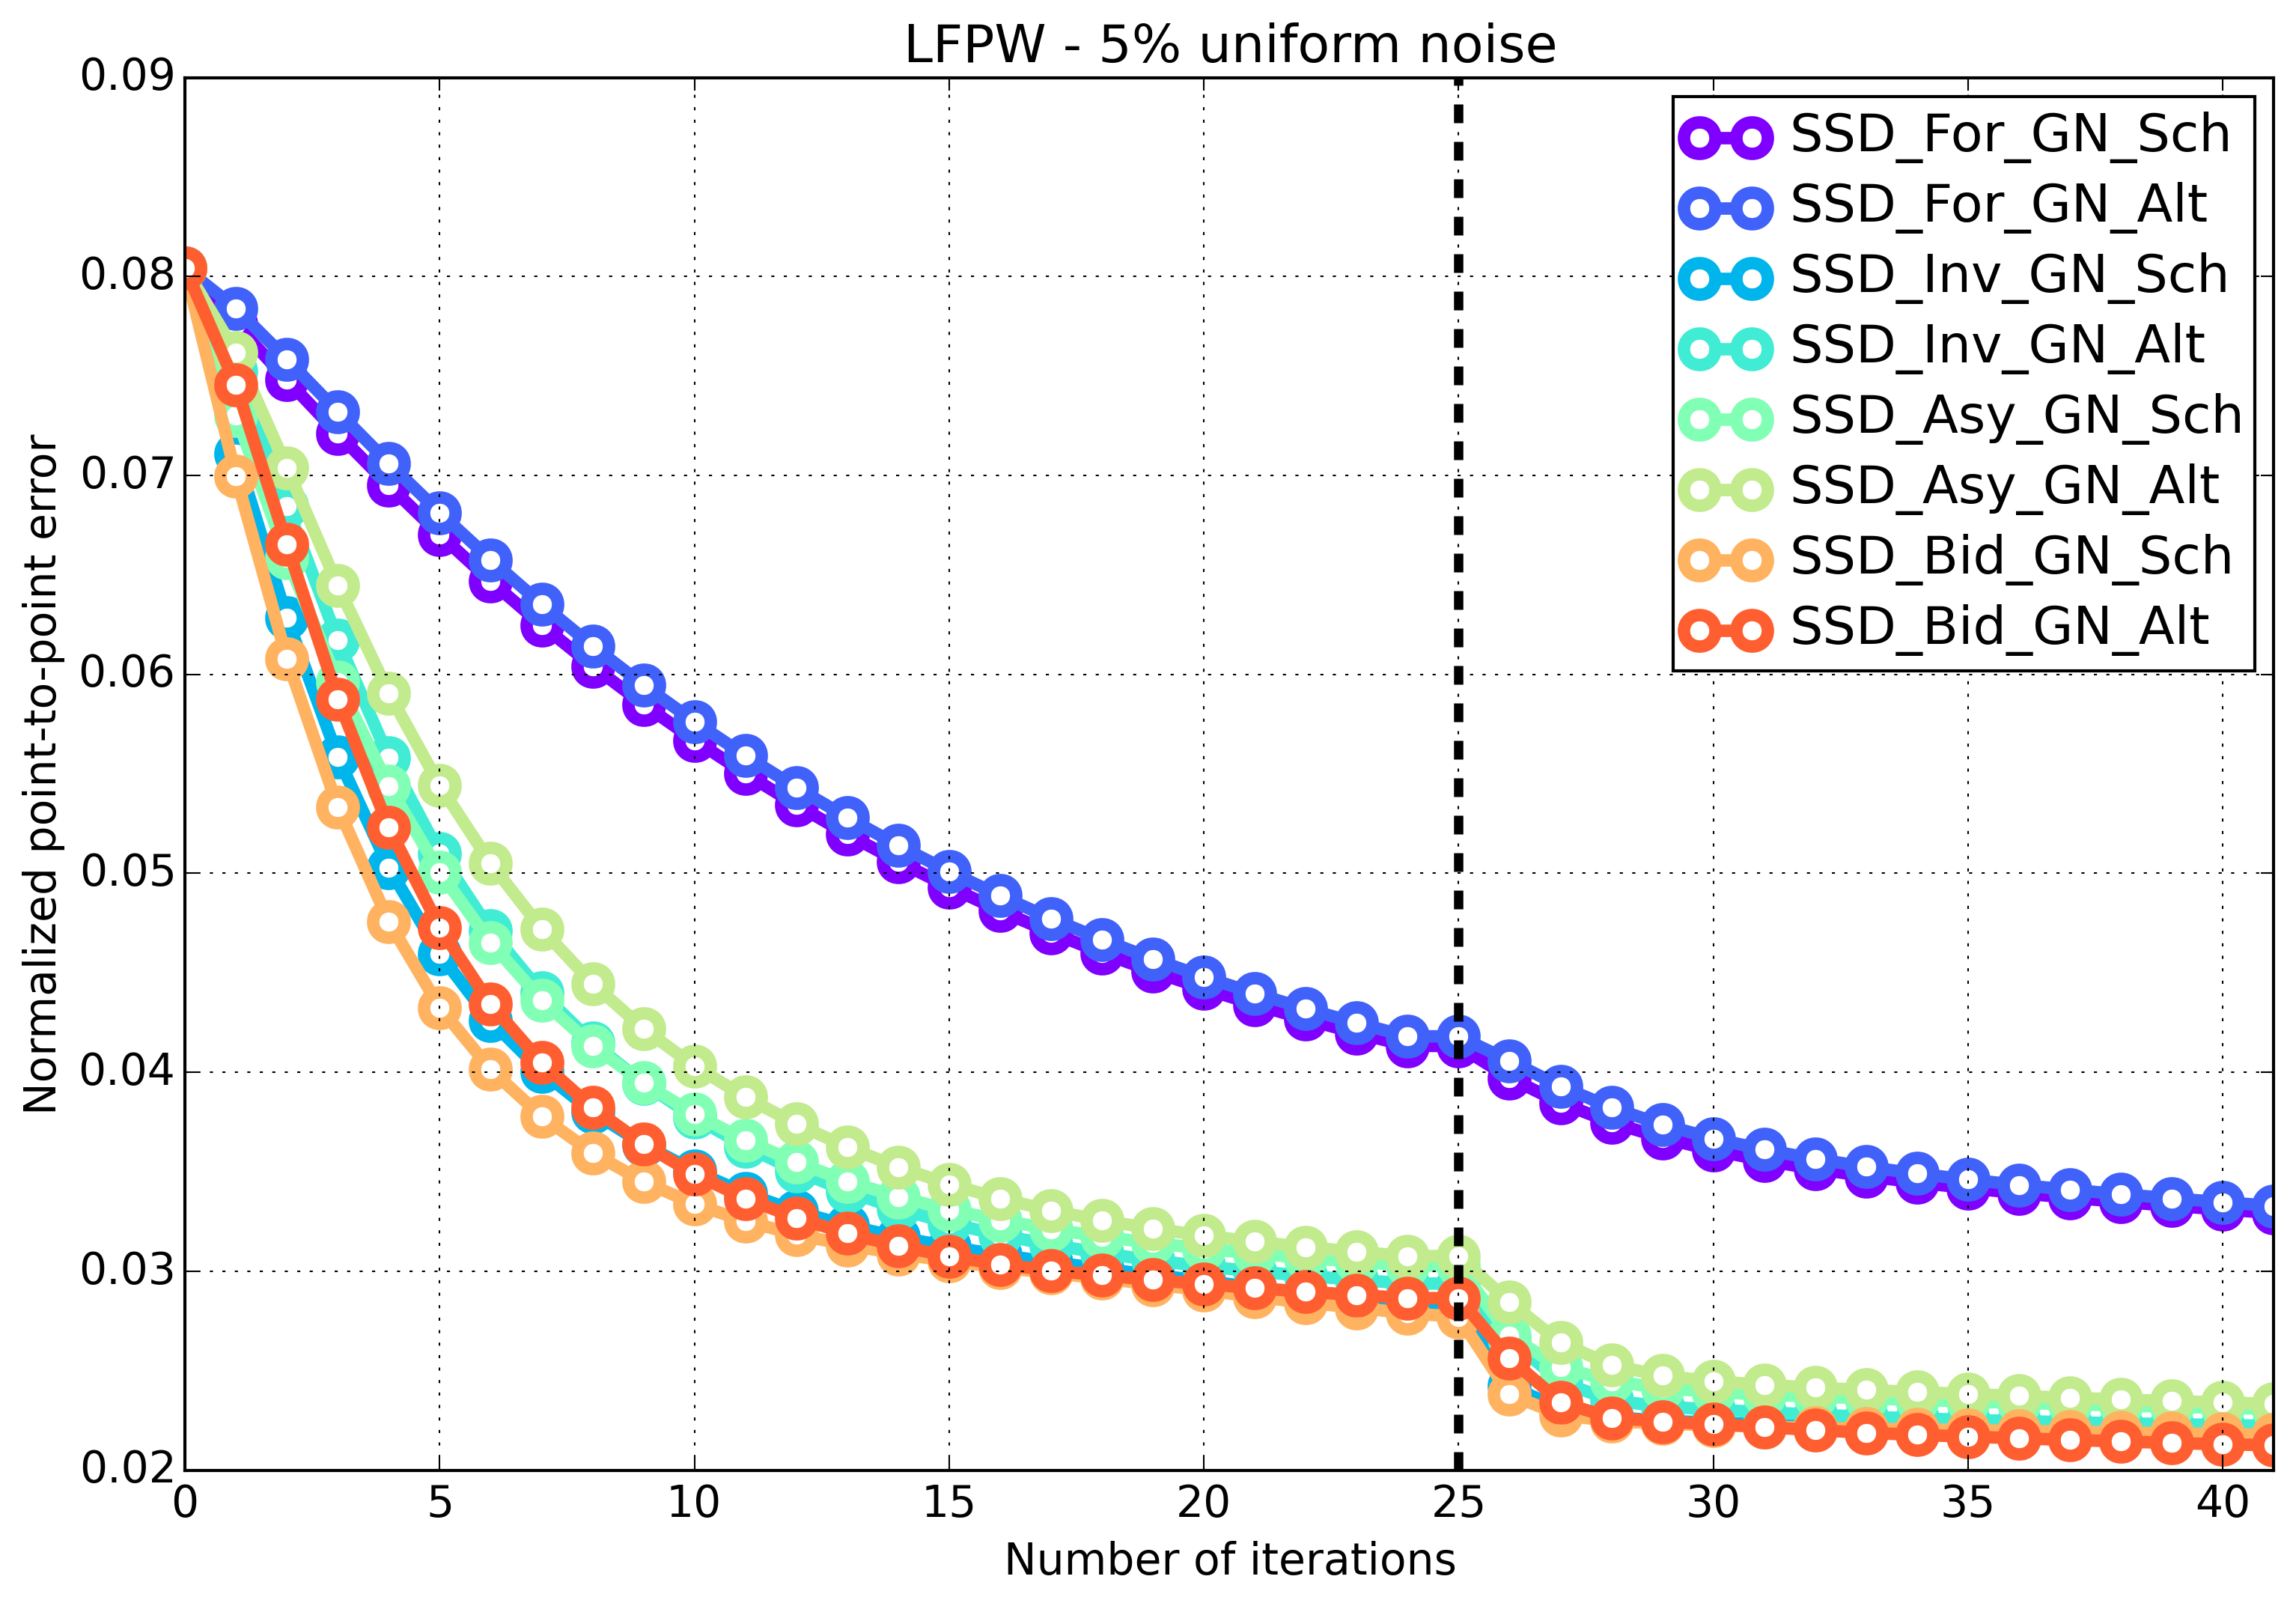
\includegraphics[width=\textwidth]{experiments/algorithms/ssd_gn/mean_error_vs_iters_ssd_gn_5.png}
	    \caption{Mean normalized point-to-point error vs number of iterations graph on the LFPW test dataset for all SSD Gauss-Newton algorithms initialized with $5\%$ uniform noise.}
	    \label{fig:mean_error_vs_iters_ssd_gn_5}
	\end{subfigure}
	\par\medskip
	\begin{subfigure}{0.48\textwidth}
	    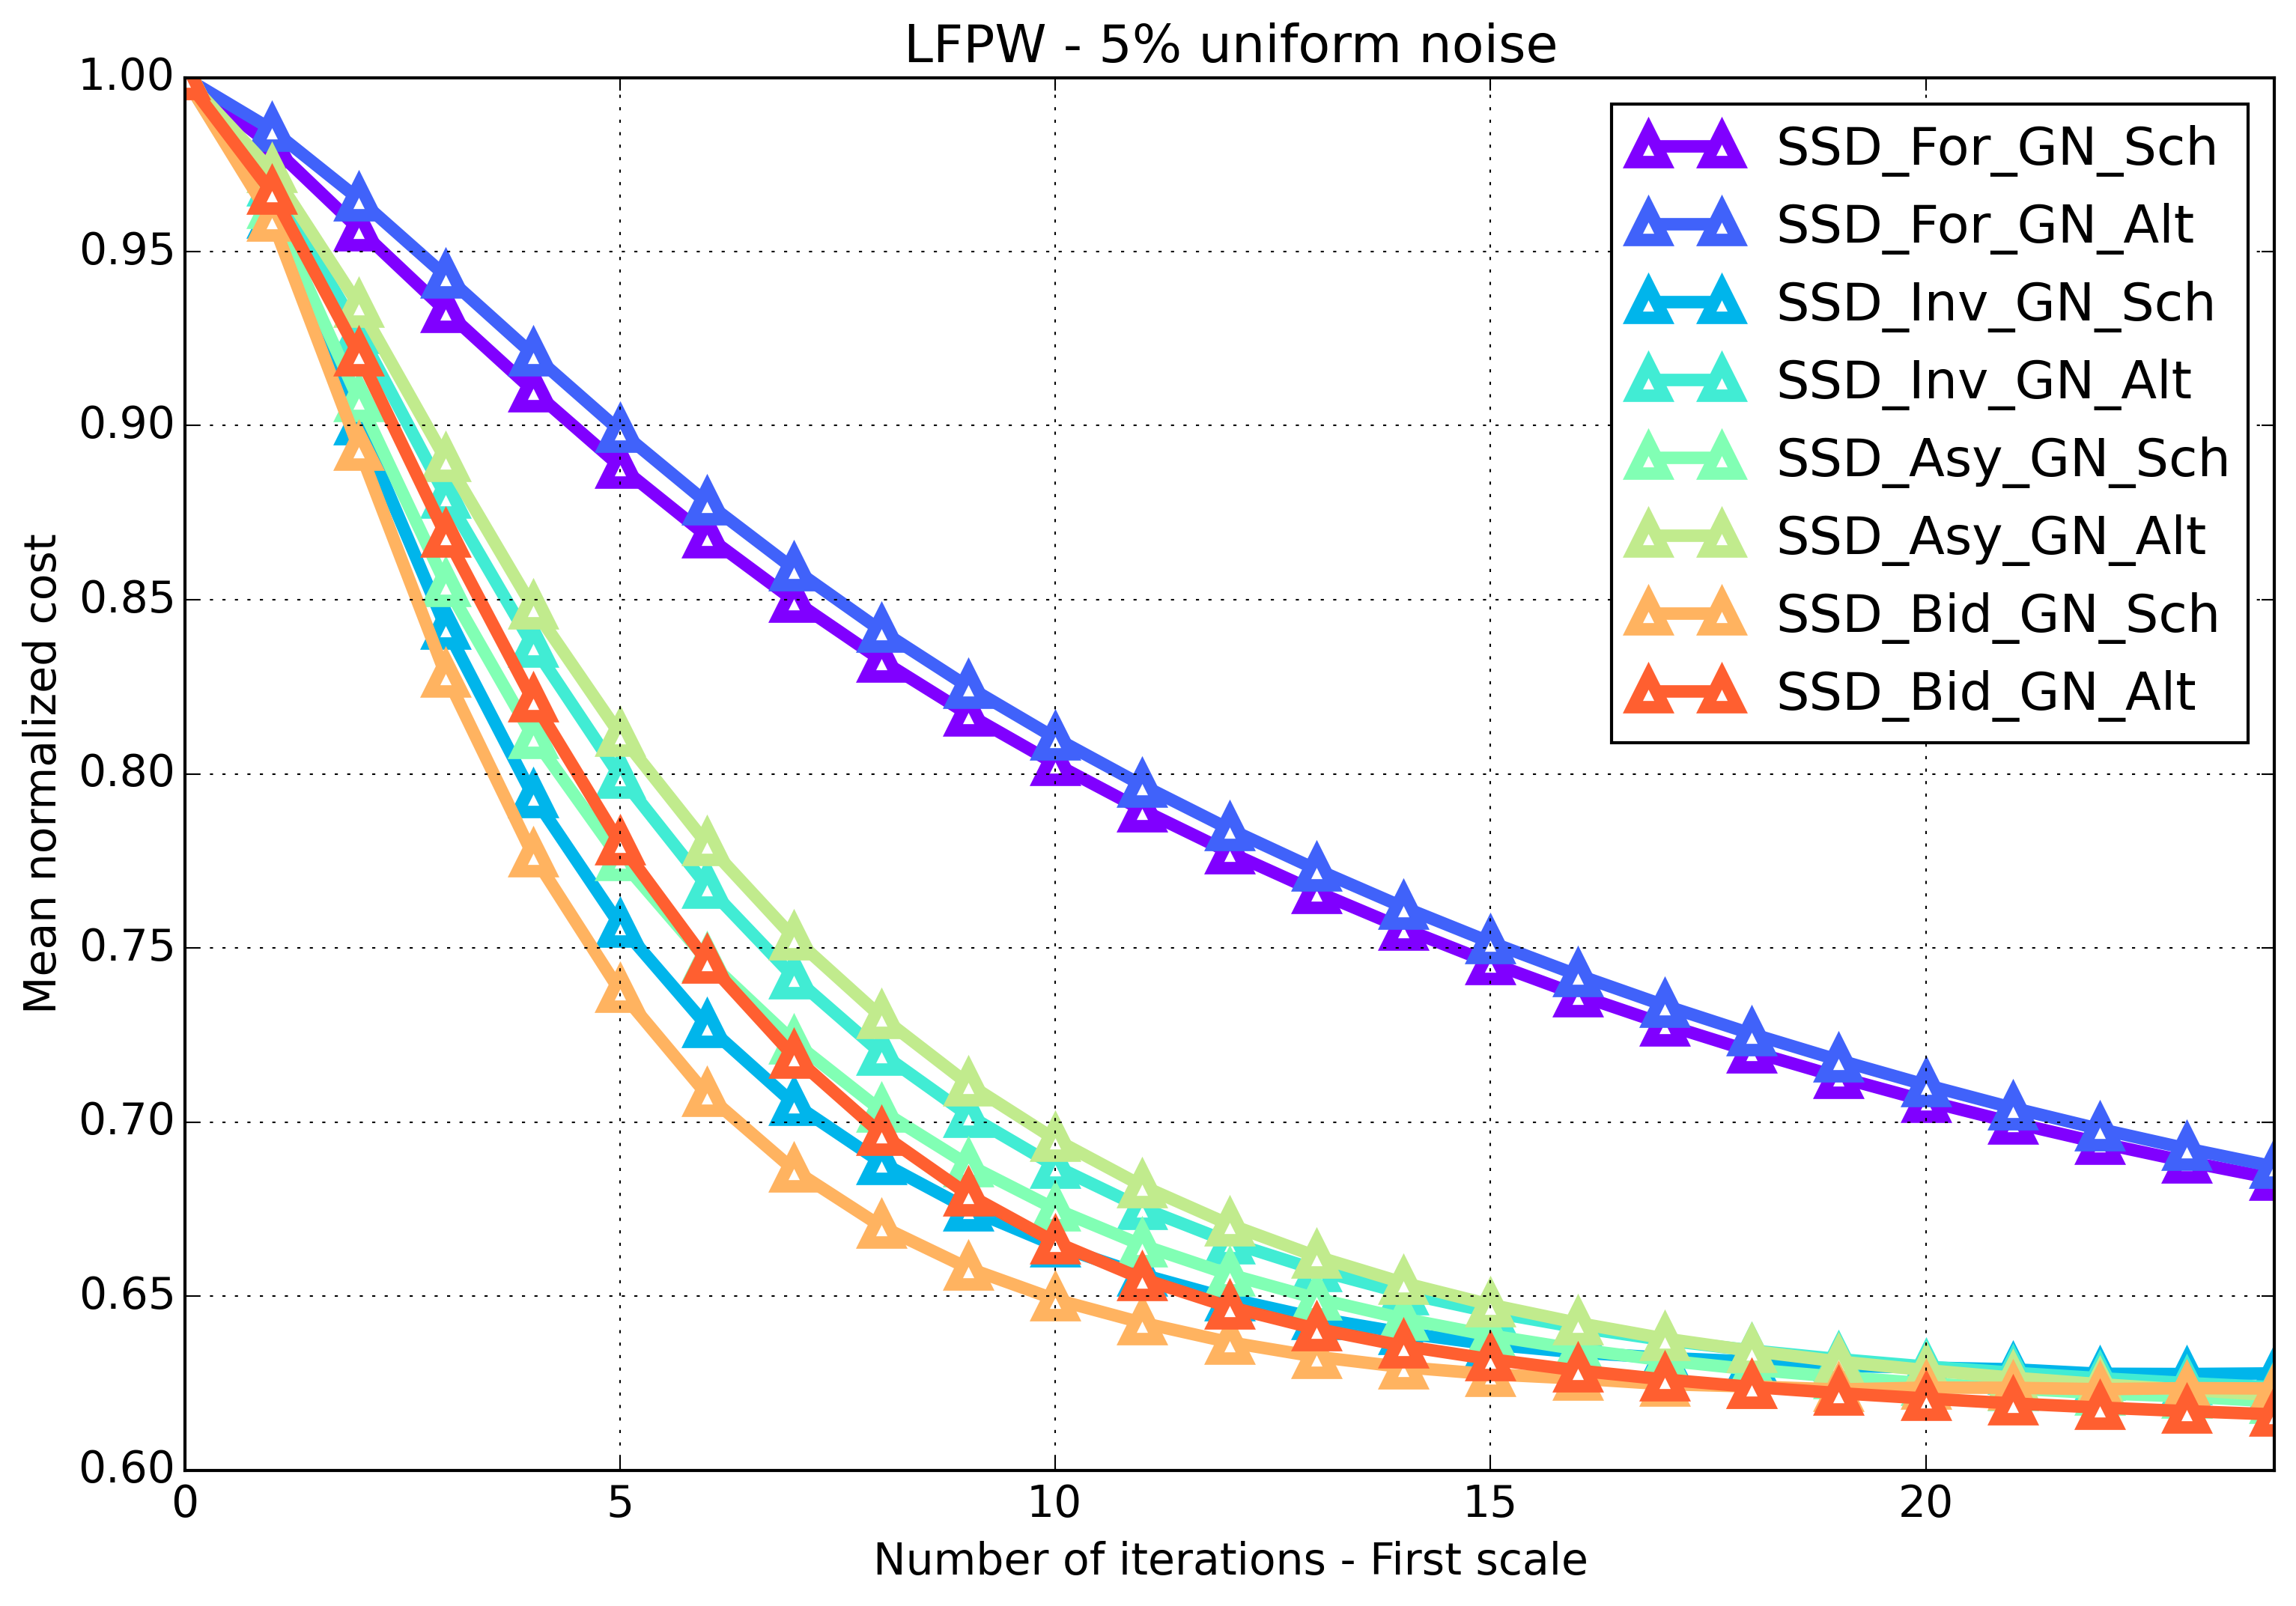
\includegraphics[width=\textwidth]{experiments/algorithms/ssd_gn/mean_cost_vs_iters1_ssd_gn_5.png}
	    \caption{Mean normalized cost vs number of first scale iterations graph on the LFPW test dataset for all SSD Gauss-Newton algorithms initialized with $5\%$ uniform noise.}
	    \label{fig:mean_cost_vs_iters1_ssd_gn_5}
	\end{subfigure}
	\hfill
	\begin{subfigure}{0.48\textwidth}
	    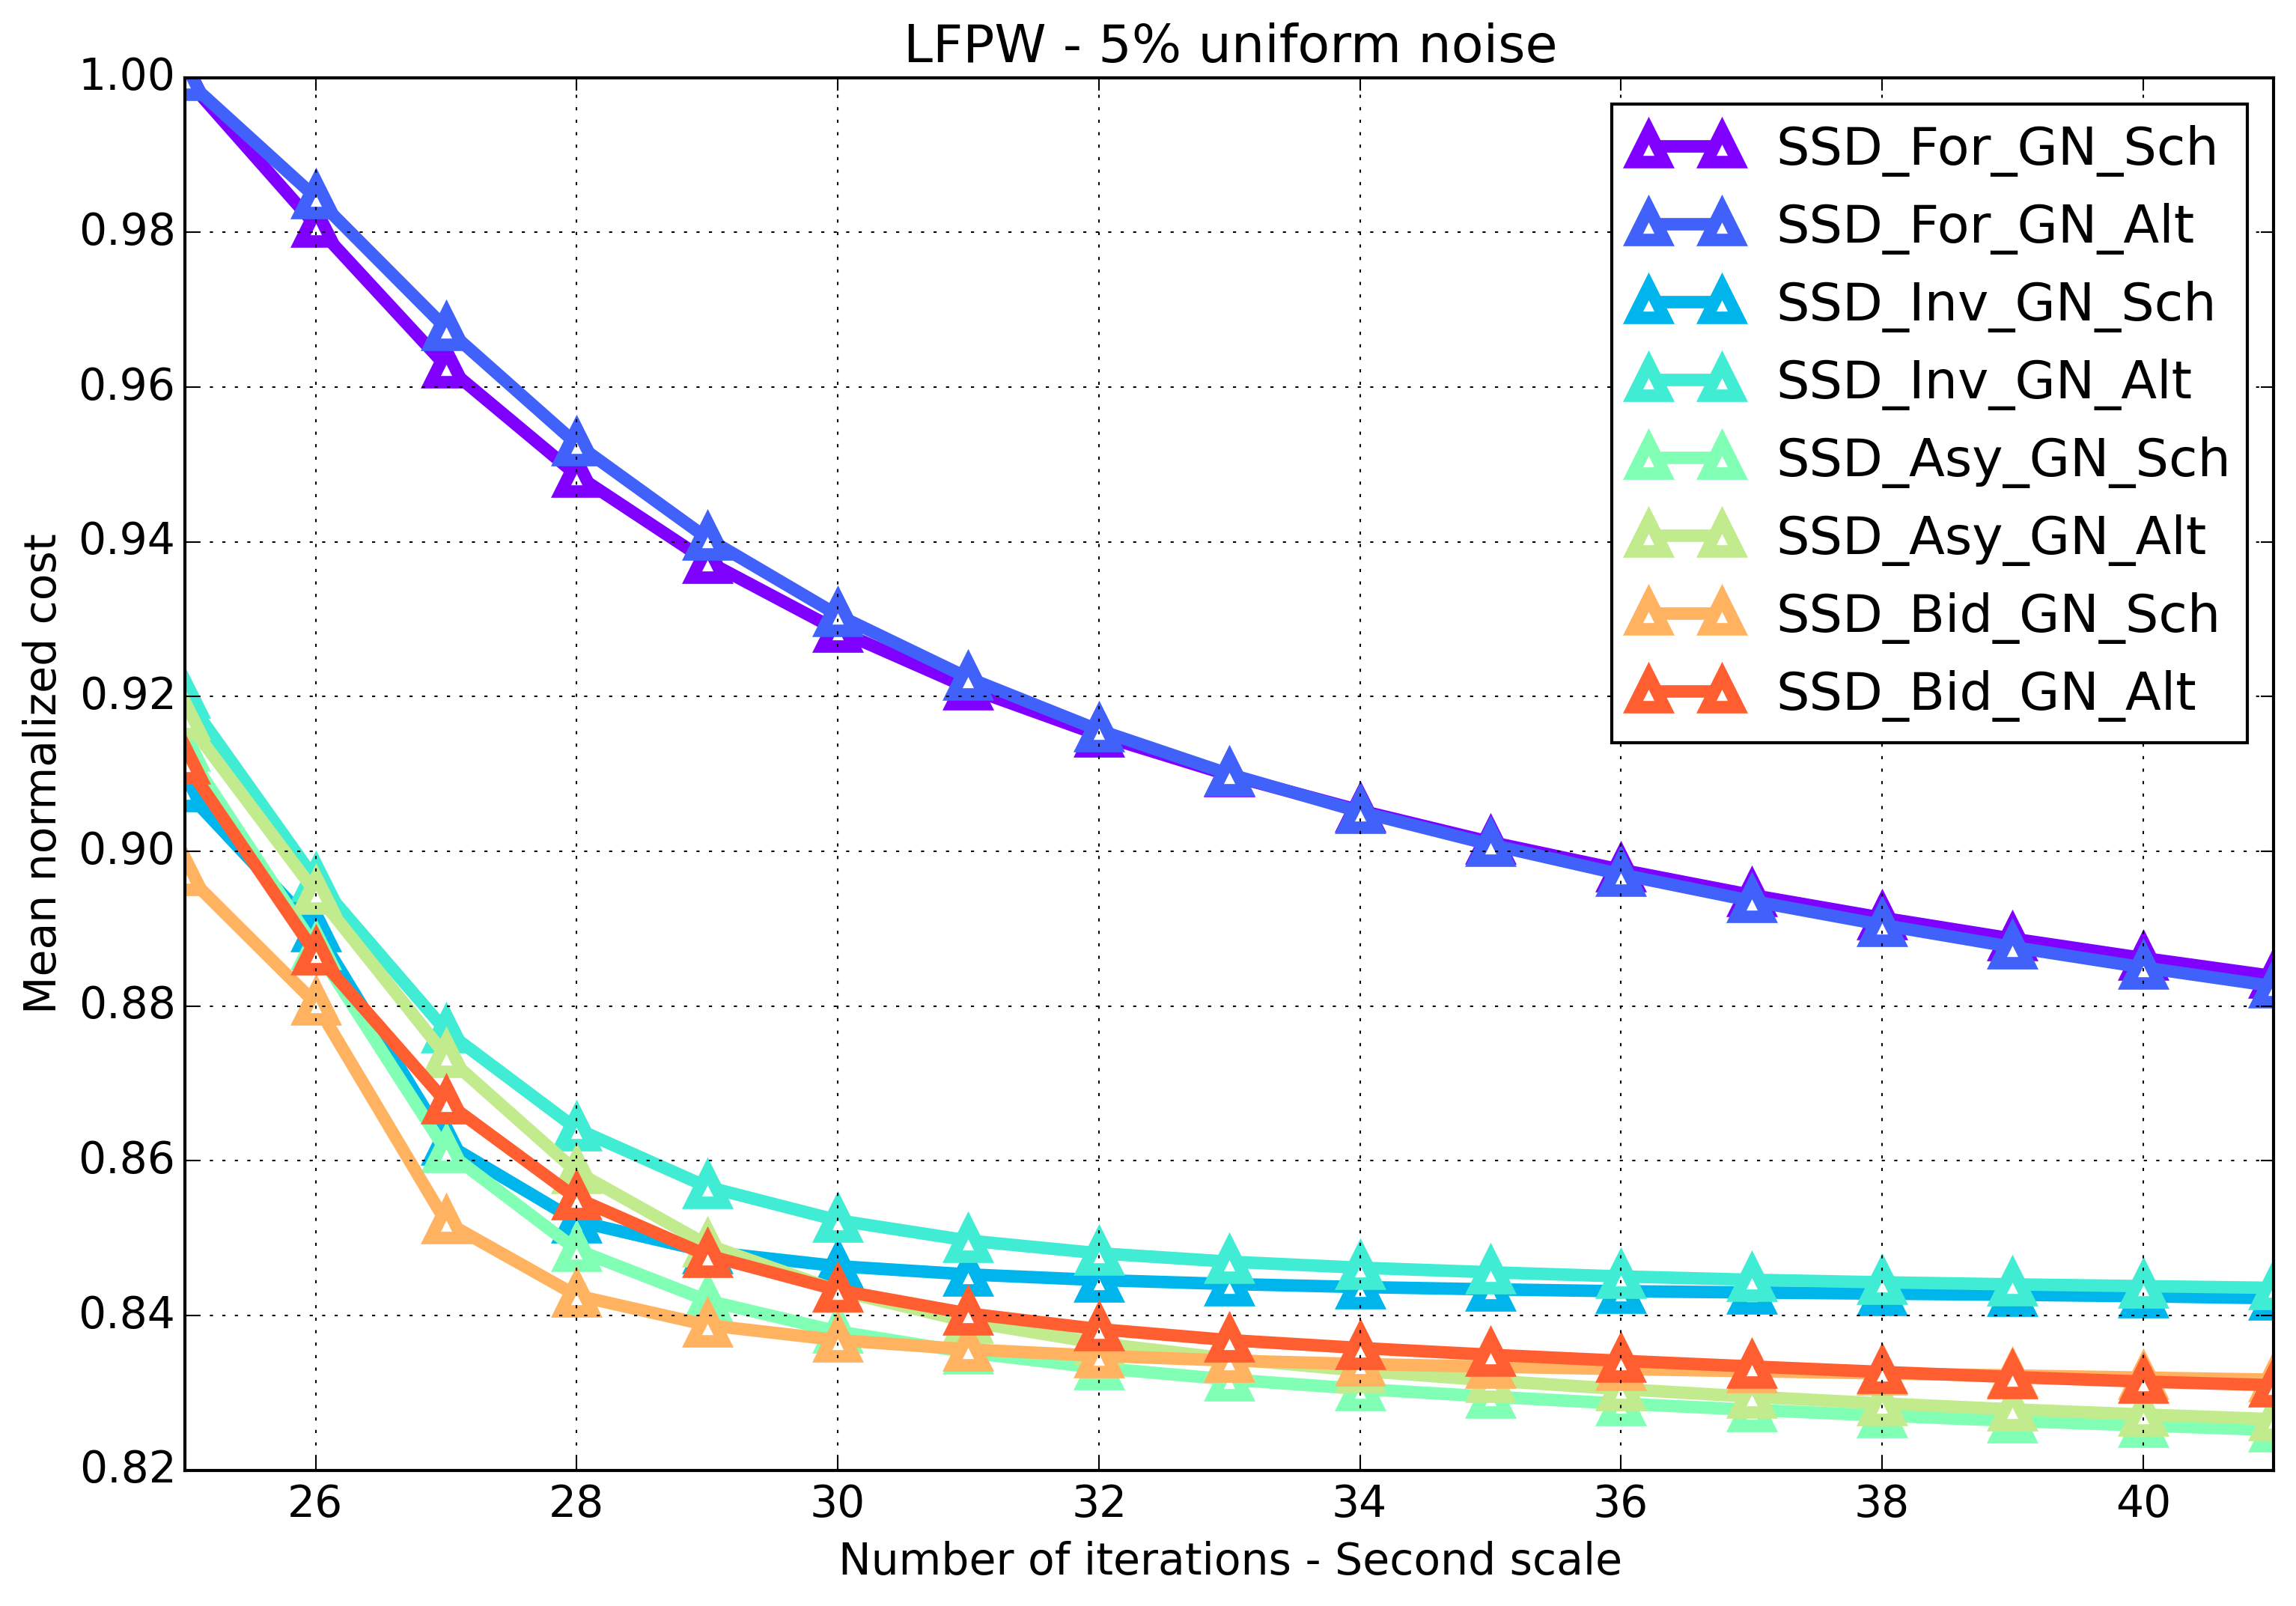
\includegraphics[width=\textwidth]{experiments/algorithms/ssd_gn/mean_cost_vs_iters2_ssd_gn_5.png}
	    \caption{Mean normalized cost vs number of second scale iterations graph on the LFPW test dataset for all SSD Gauss-Newton algorithms initialized with $5\%$ uniform noise.}
	    \label{fig:mean_cost_vs_iters2_ssd_gn_5}
	\end{subfigure}
	\label{fig:ssd_gn_5}
	\caption{}
\end{figure*}


\subsubsection*{Wiberg}

\begin{figure*}[h!]
	\centering
	\begin{subfigure}{0.48\textwidth}
	    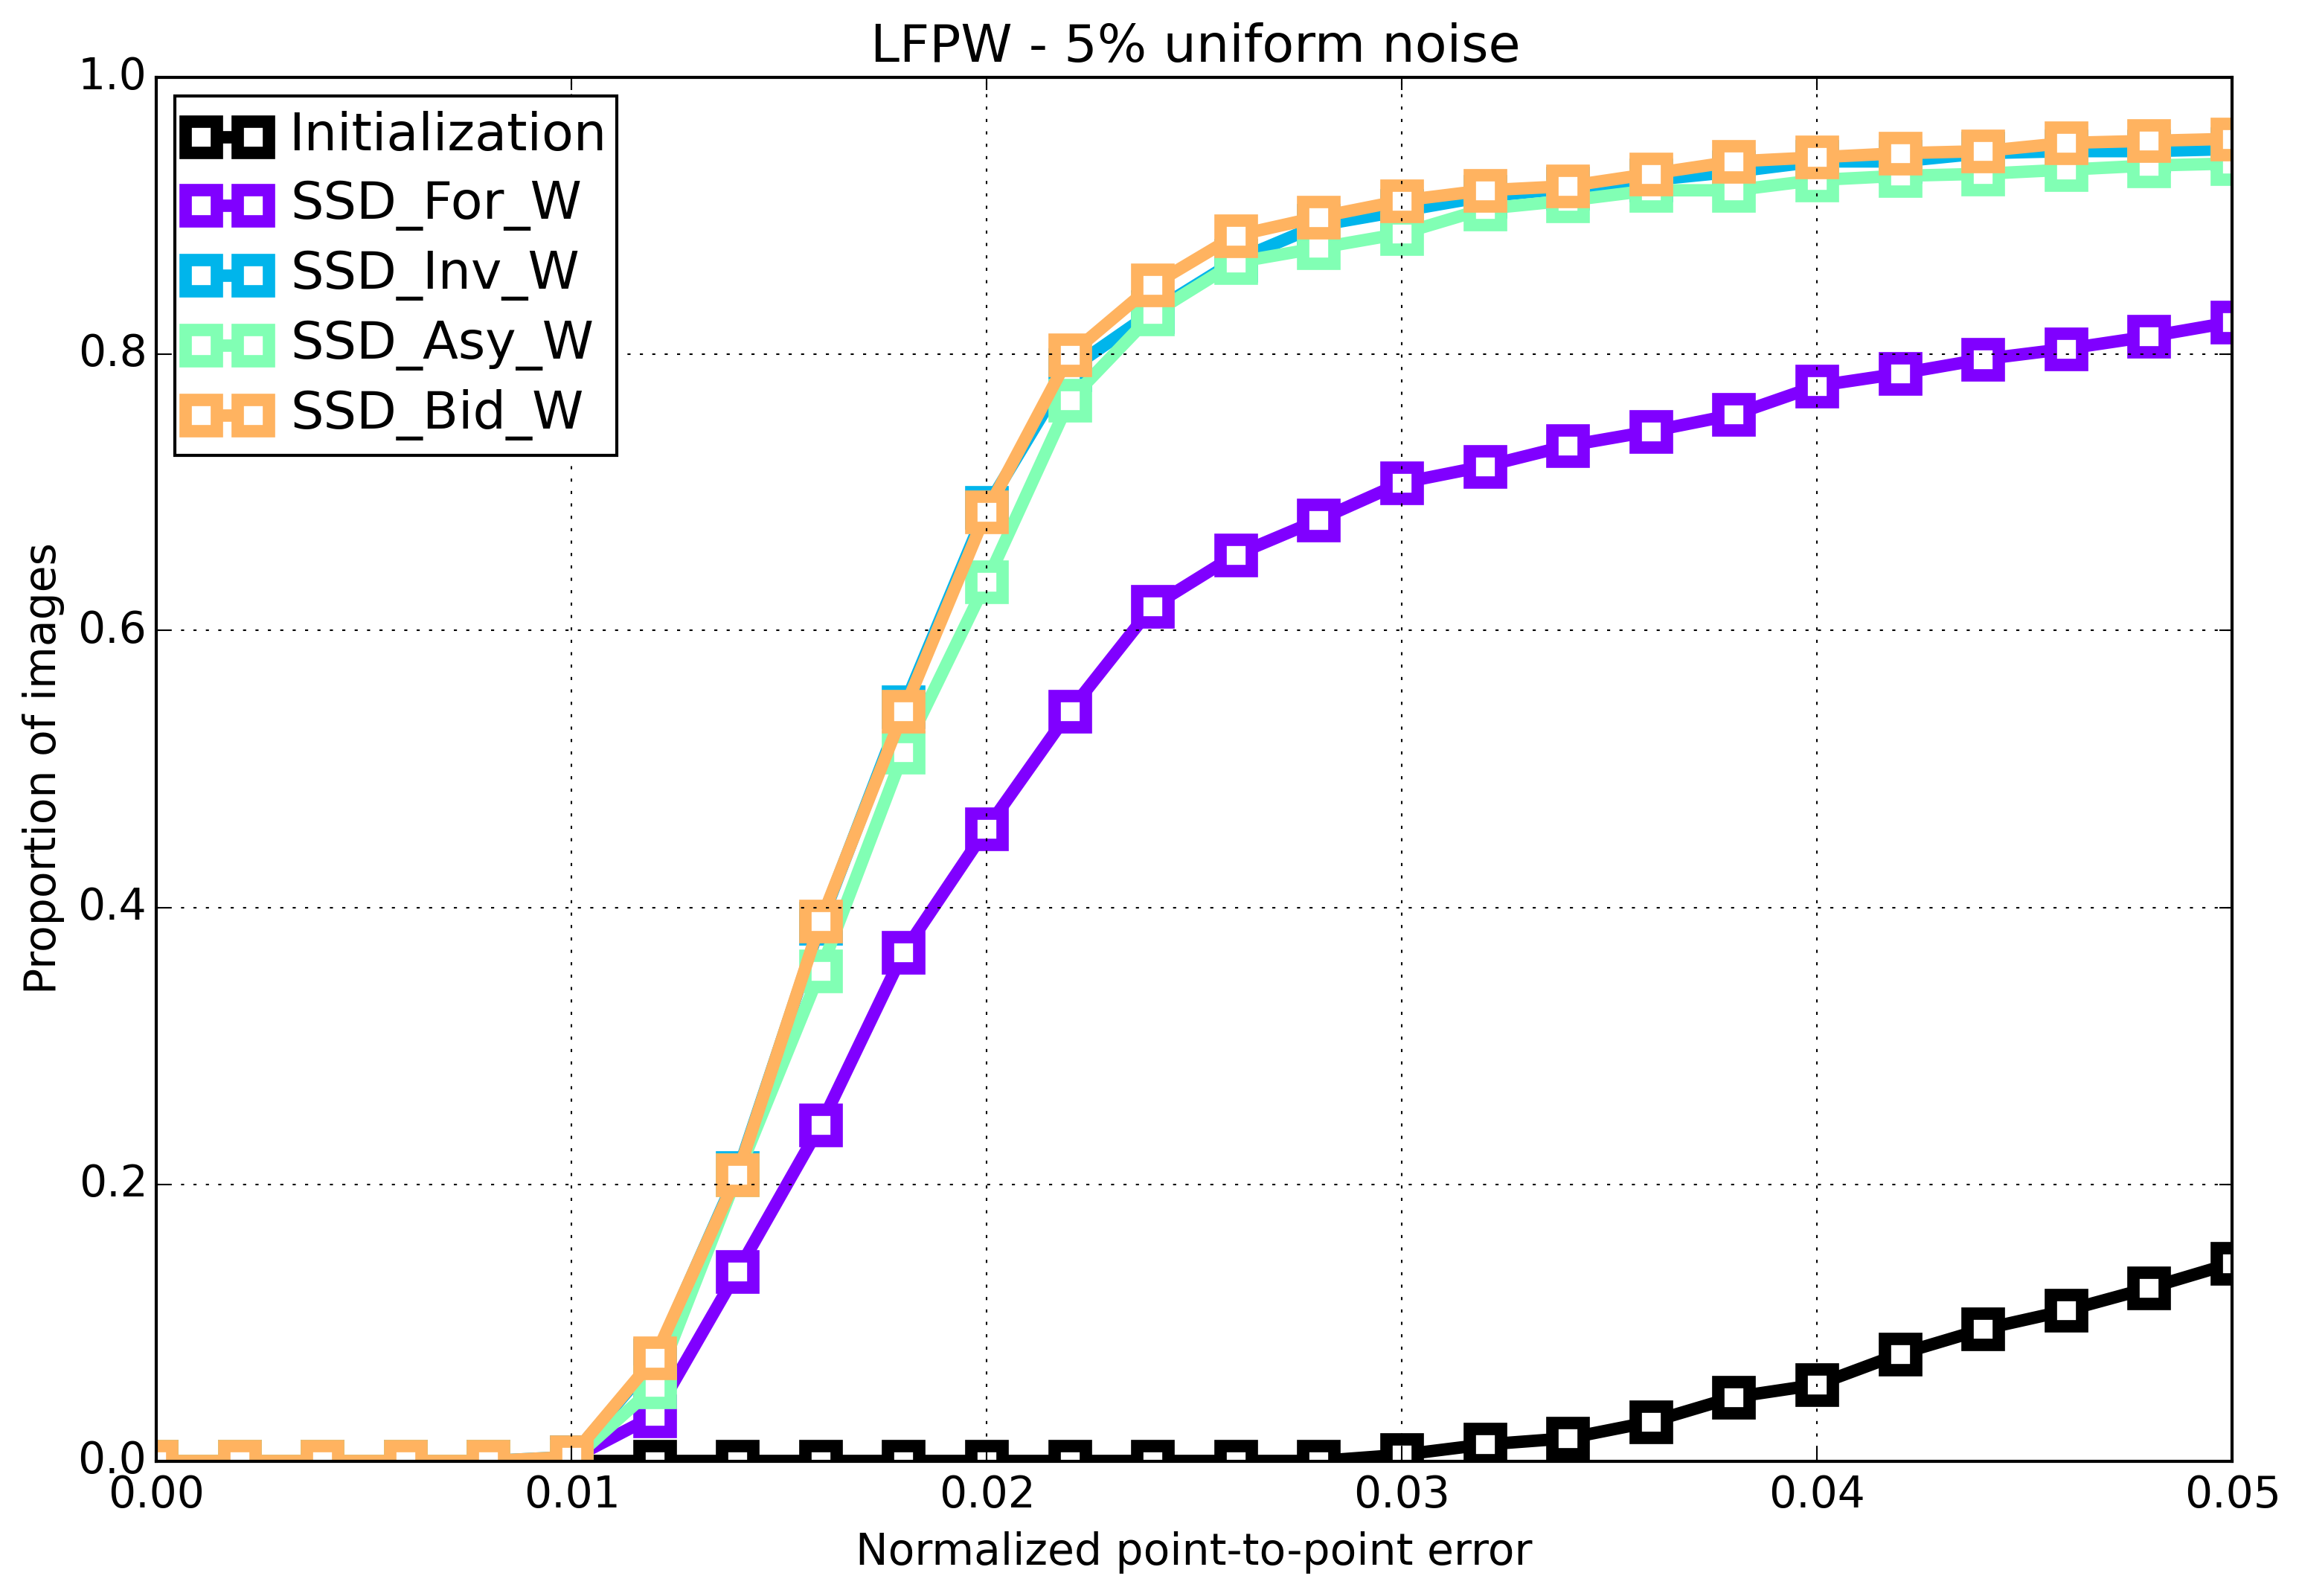
\includegraphics[width=\textwidth]{experiments/algorithms/ssd_w/ced_ssd_w_5.png}
	    \caption{Cumulative Error Distribution graph on the LFPW test dataset for all SSD Wiberg algorithms initialized with $5\%$ uniform noise.}
	    \label{fig:ced_ssd_w_5}
	\end{subfigure}
	\hfill
	\begin{subfigure}{0.48\textwidth}
	    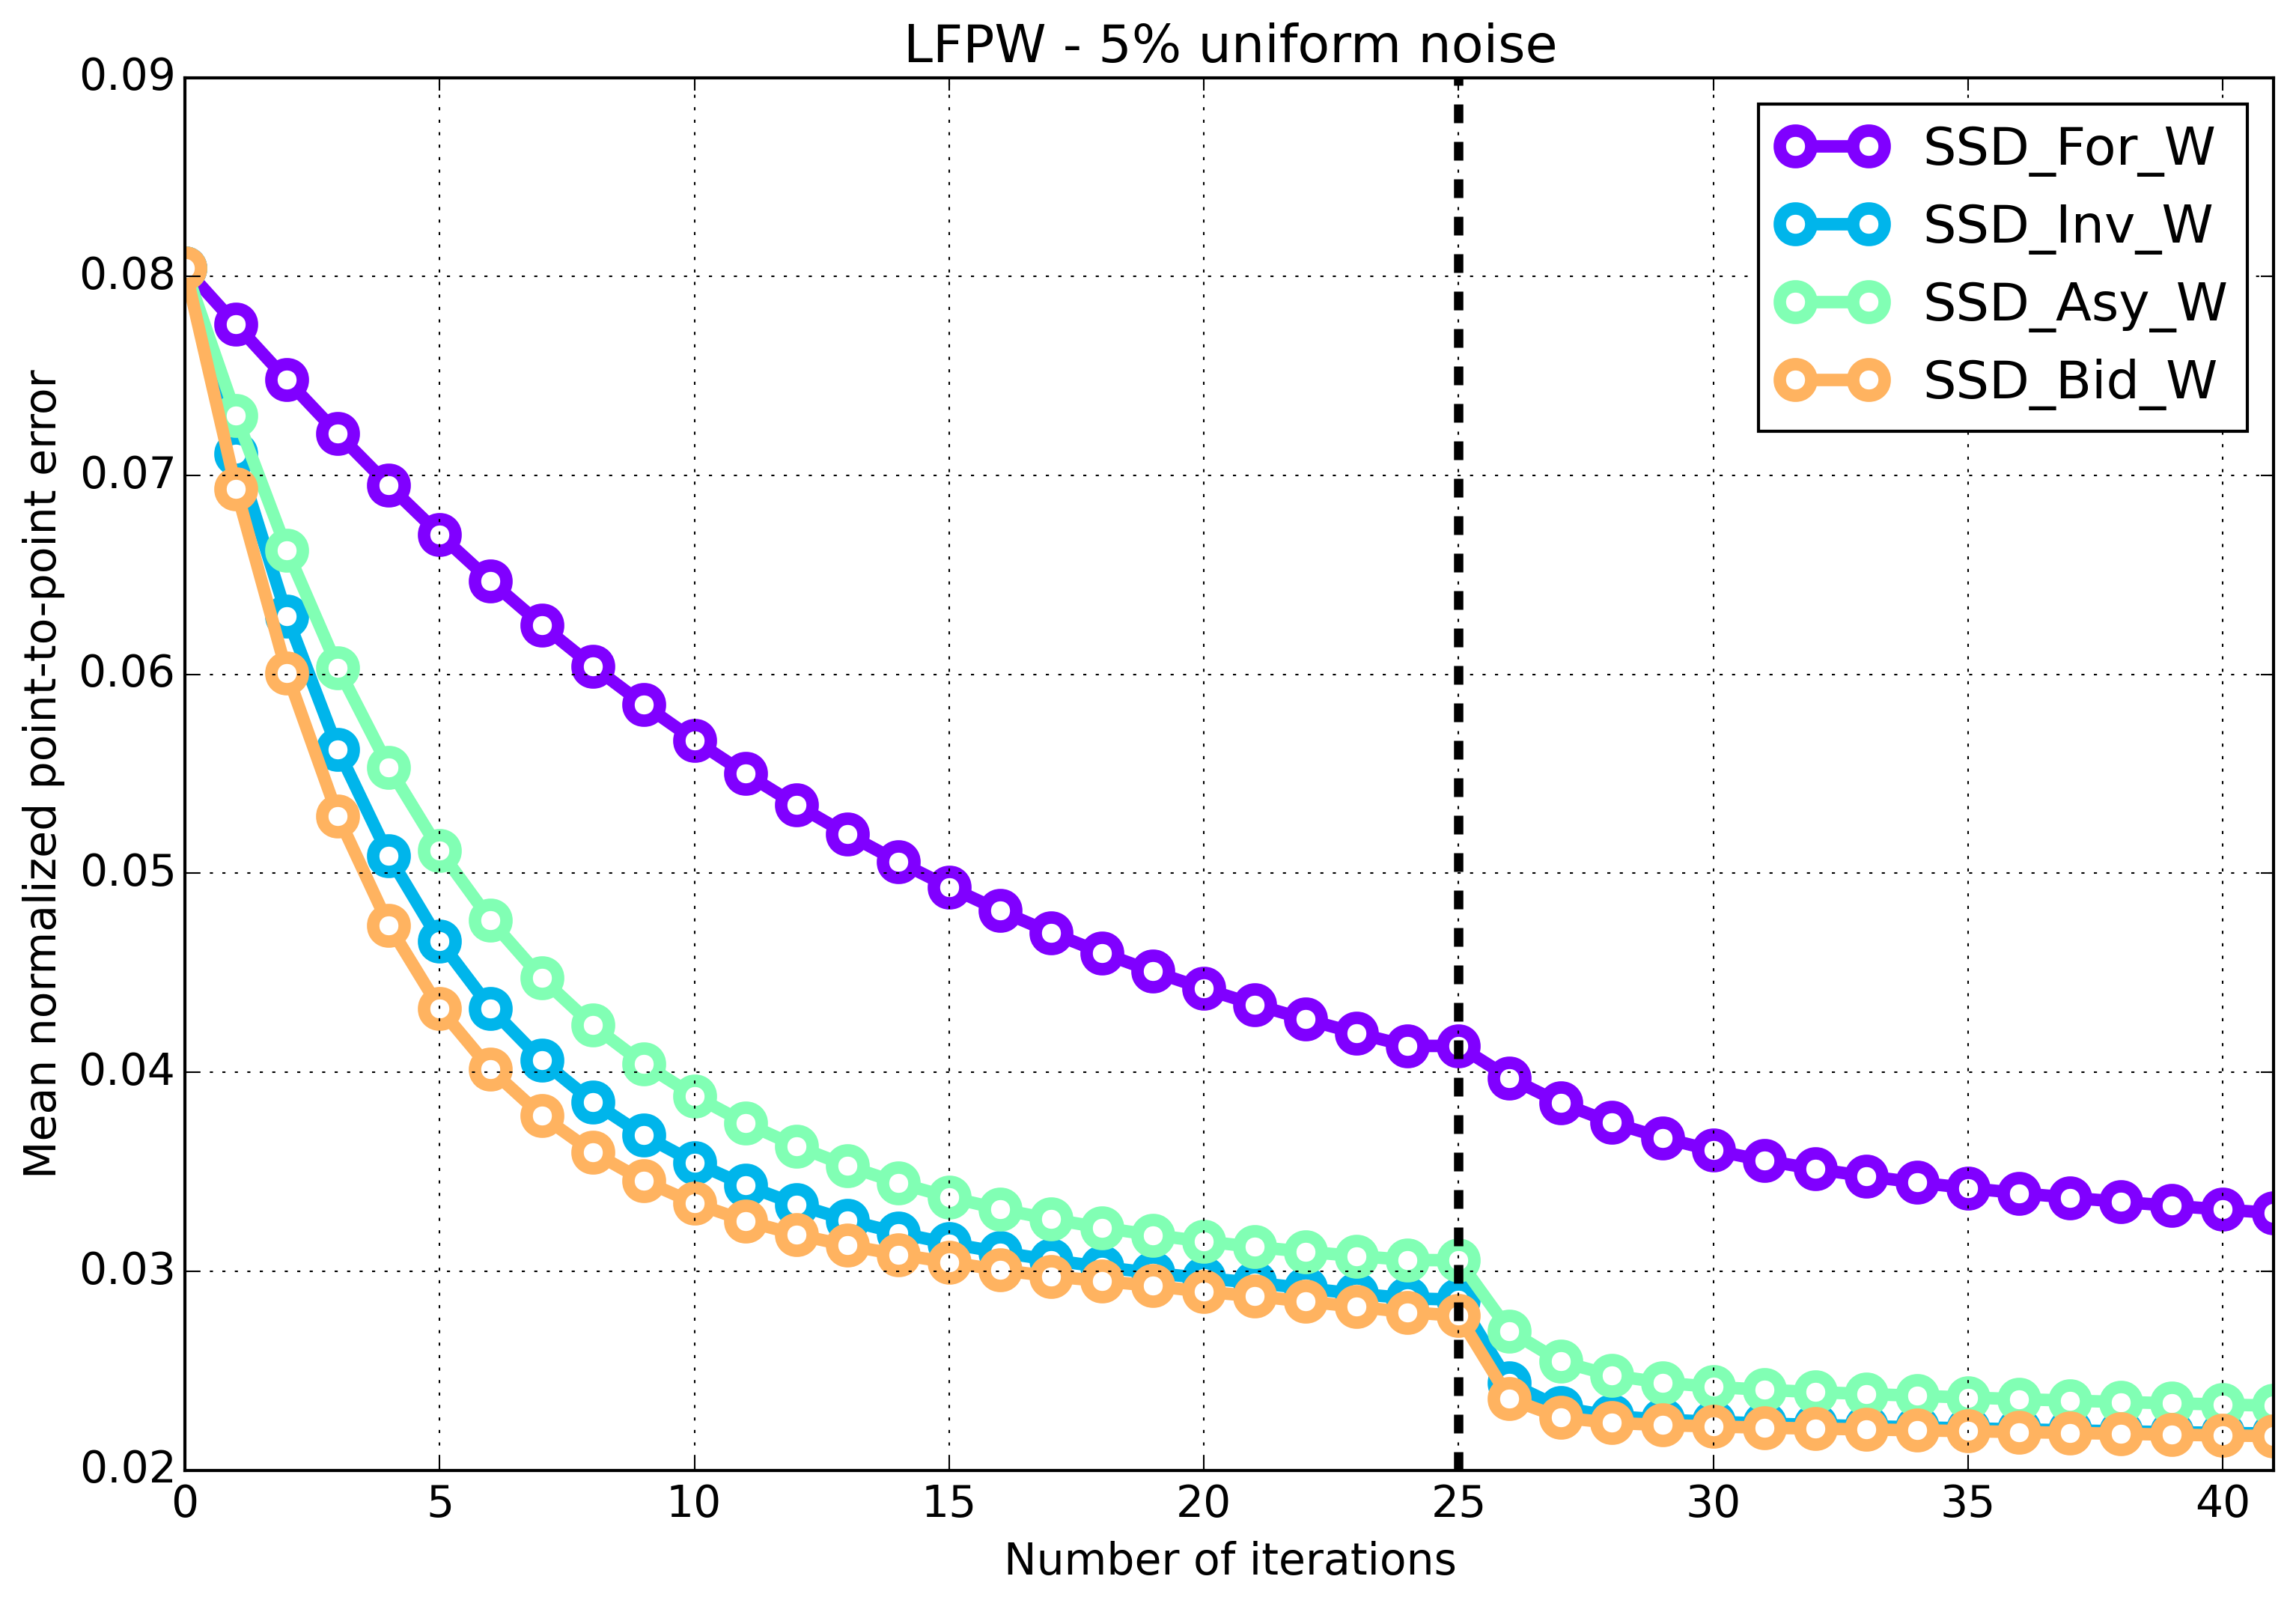
\includegraphics[width=\textwidth]{experiments/algorithms/ssd_w/mean_error_vs_iters_ssd_w_5.png}
	    \caption{Mean normalized point-to-point error vs number of iterations graph on the LFPW test dataset for all SSD Wiberg algorithms initialized with $5\%$ uniform noise.}
	    \label{fig:mean_error_vs_iters_ssd_w_5}
	\end{subfigure}
	\par\medskip
	\begin{subfigure}{0.48\textwidth}
	    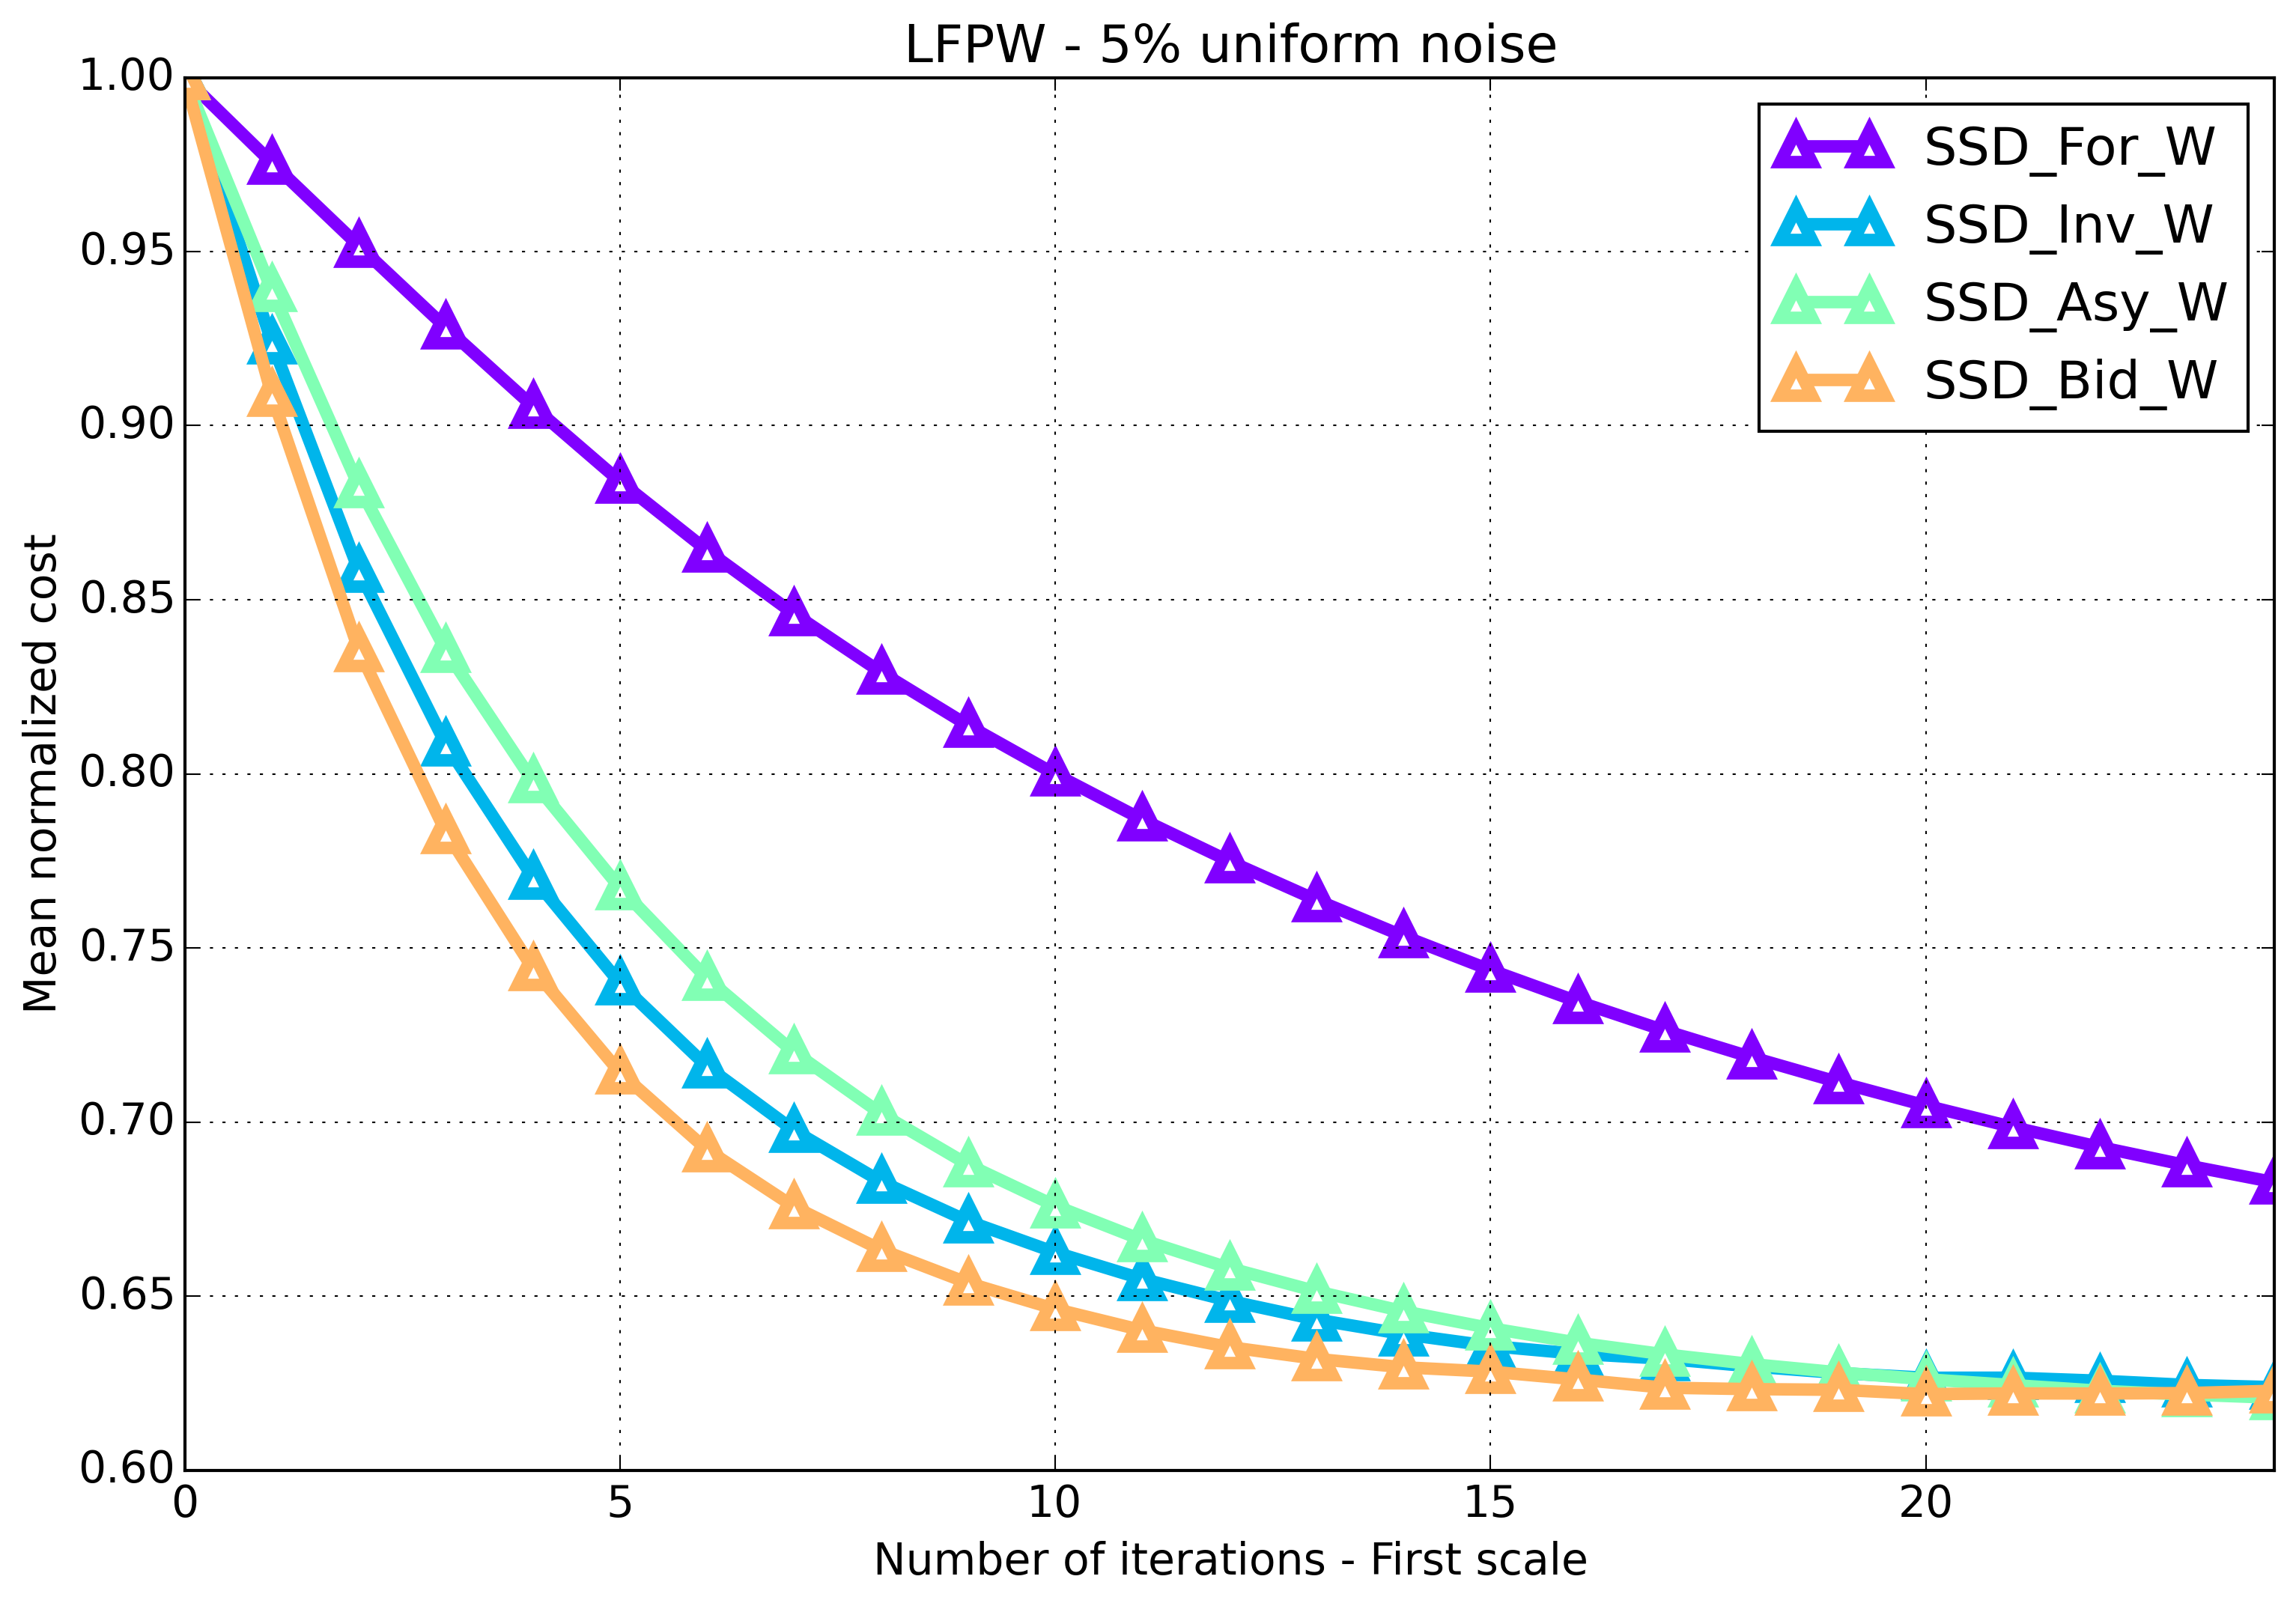
\includegraphics[width=\textwidth]{experiments/algorithms/ssd_w/mean_cost_vs_iters1_ssd_w_5.png}
	    \caption{Mean normalized cost vs number of first scale iterations graph on the LFPW test dataset for all SSD Wiberg algorithms initialized with $5\%$ uniform noise.}
	    \label{fig:mean_cost_vs_iters1_ssd_w_5}
	\end{subfigure}
	\hfill
	\begin{subfigure}{0.48\textwidth}
	    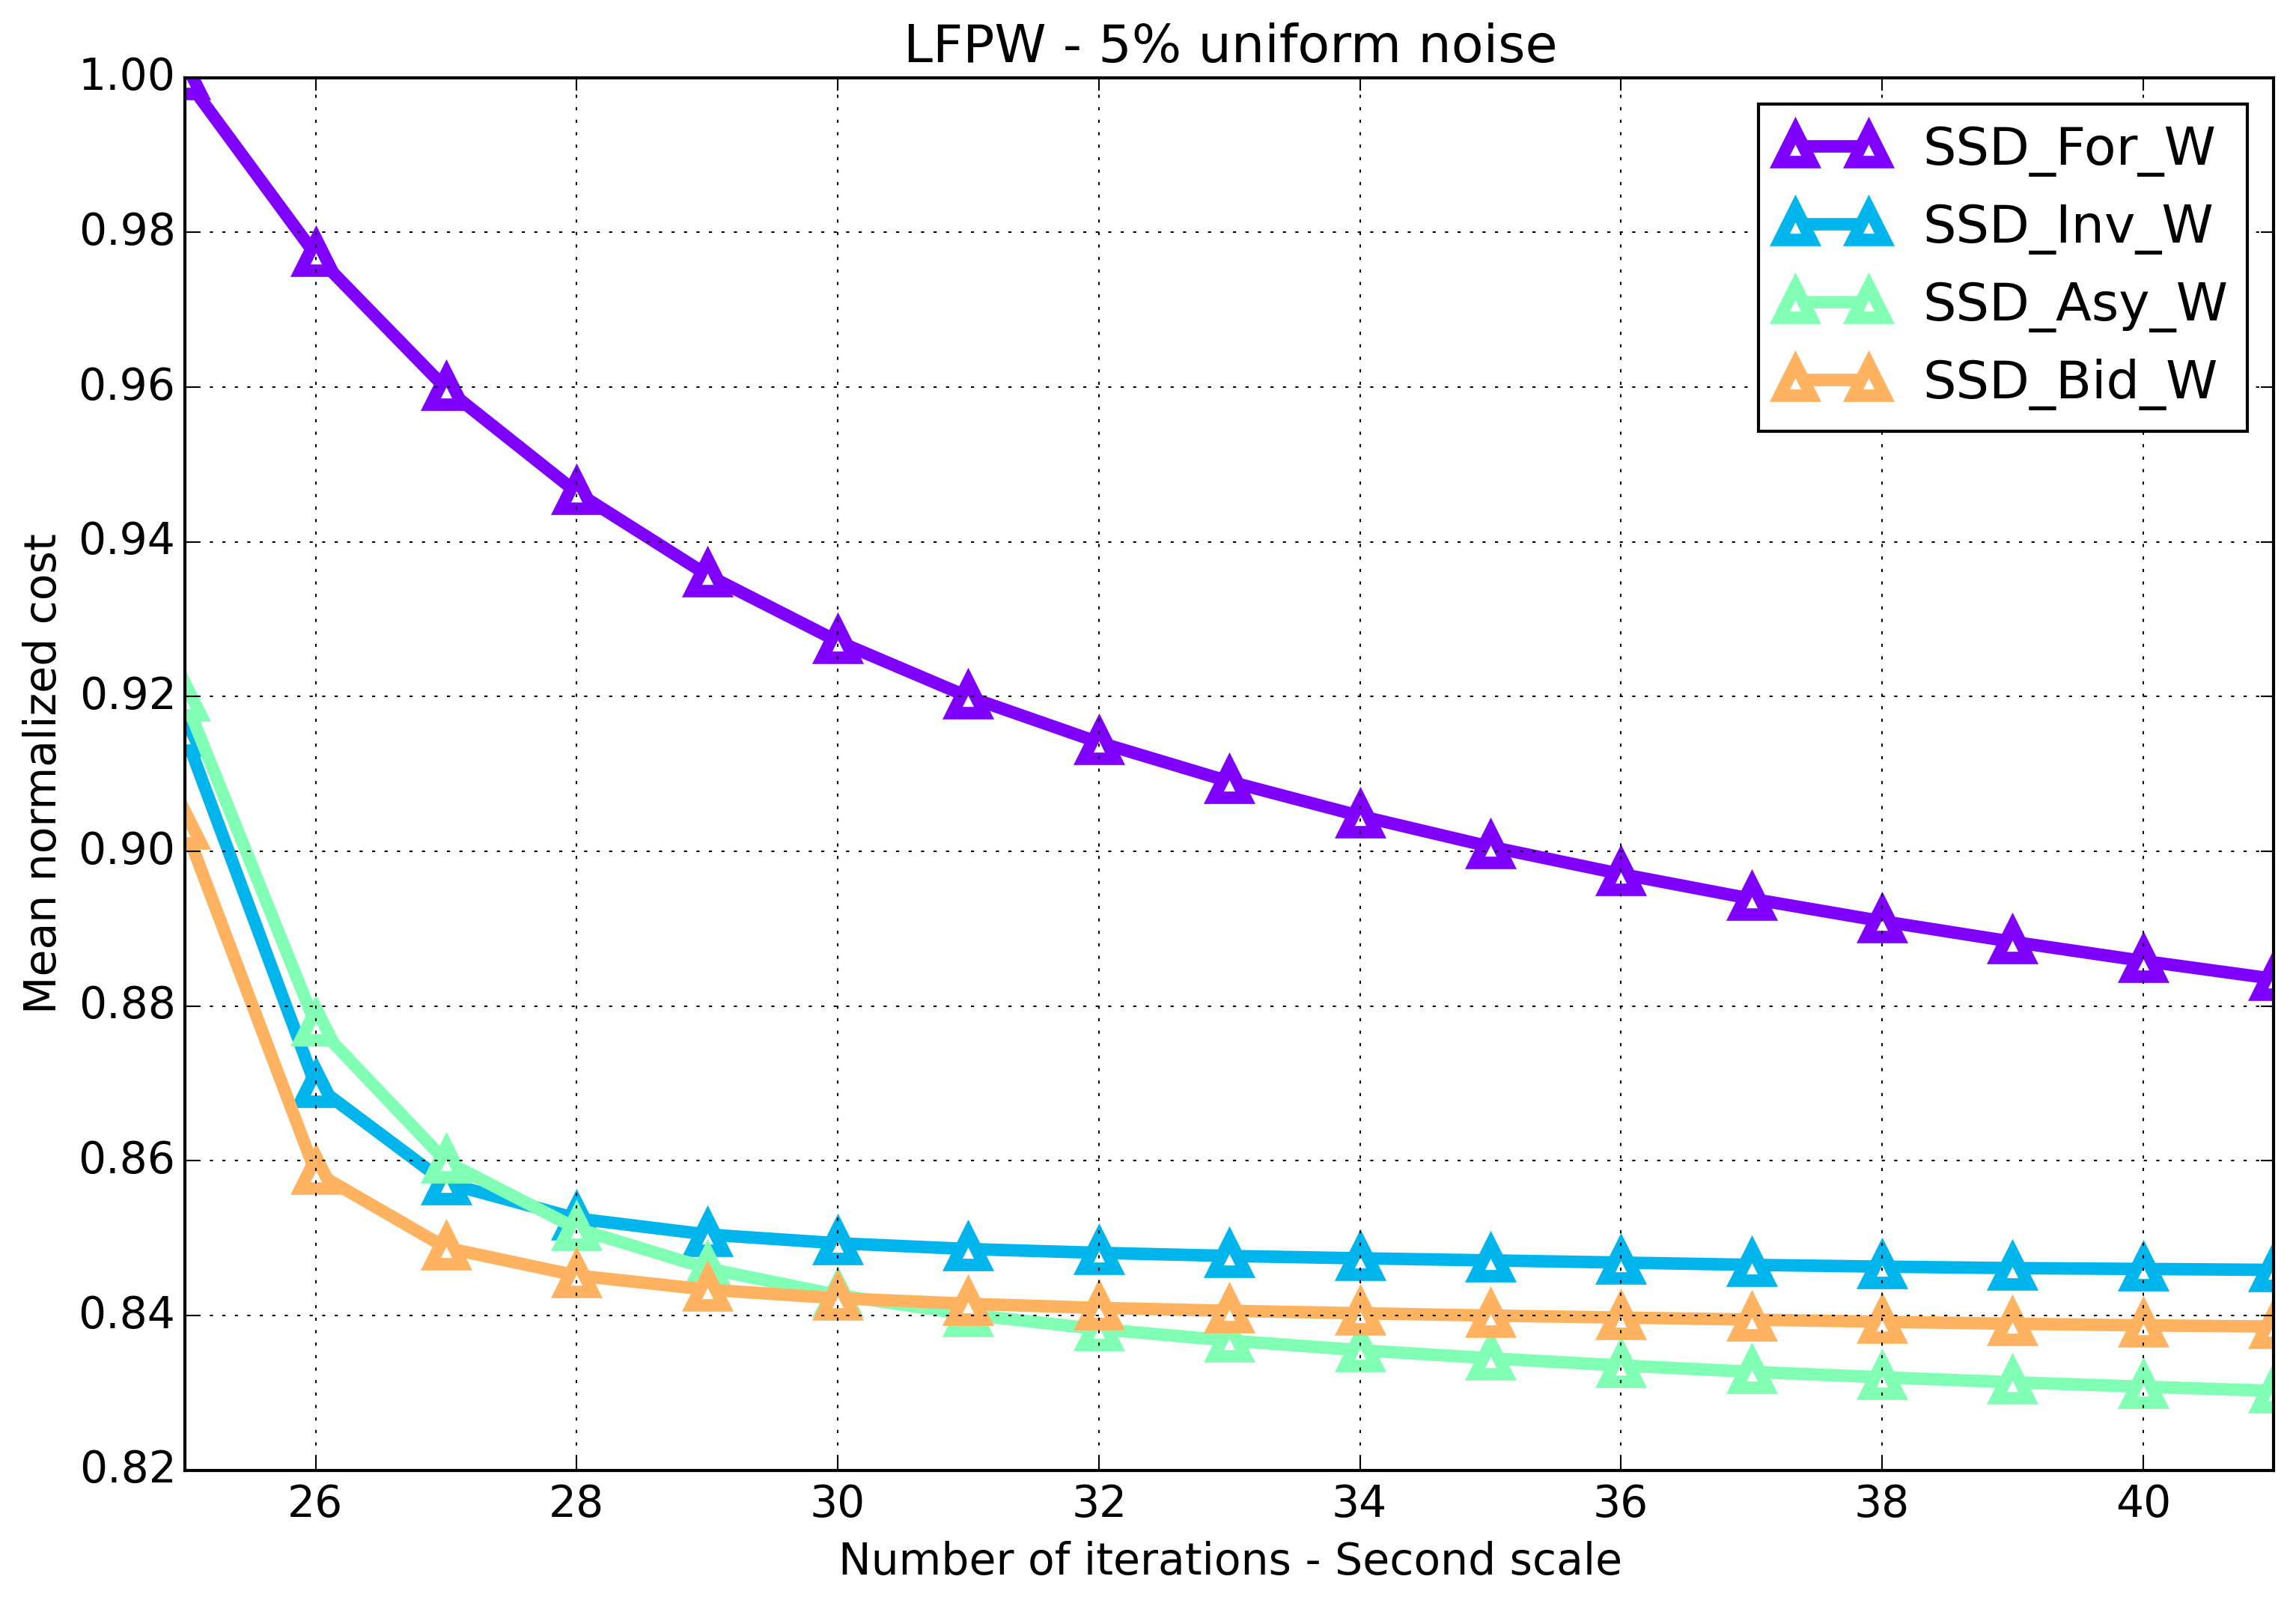
\includegraphics[width=\textwidth]{experiments/algorithms/ssd_w/mean_cost_vs_iters2_ssd_w_5.png}
	    \caption{Mean normalized cost vs number of second scale iterations graph on the LFPW test dataset for all SSD Wiberg algorithms initialized with $5\%$ uniform noise.}
	    \label{fig:mean_cost_vs_iters2_ssd_w_5}
	\end{subfigure}
	\label{fig:ssd_w_5}
	\caption{}
\end{figure*}


\subsubsection{Project-Out algorithms}


\subsubsection*{Gauss-Newton}

\begin{figure*}[h!]
	\centering
	\begin{subfigure}{0.48\textwidth}
	    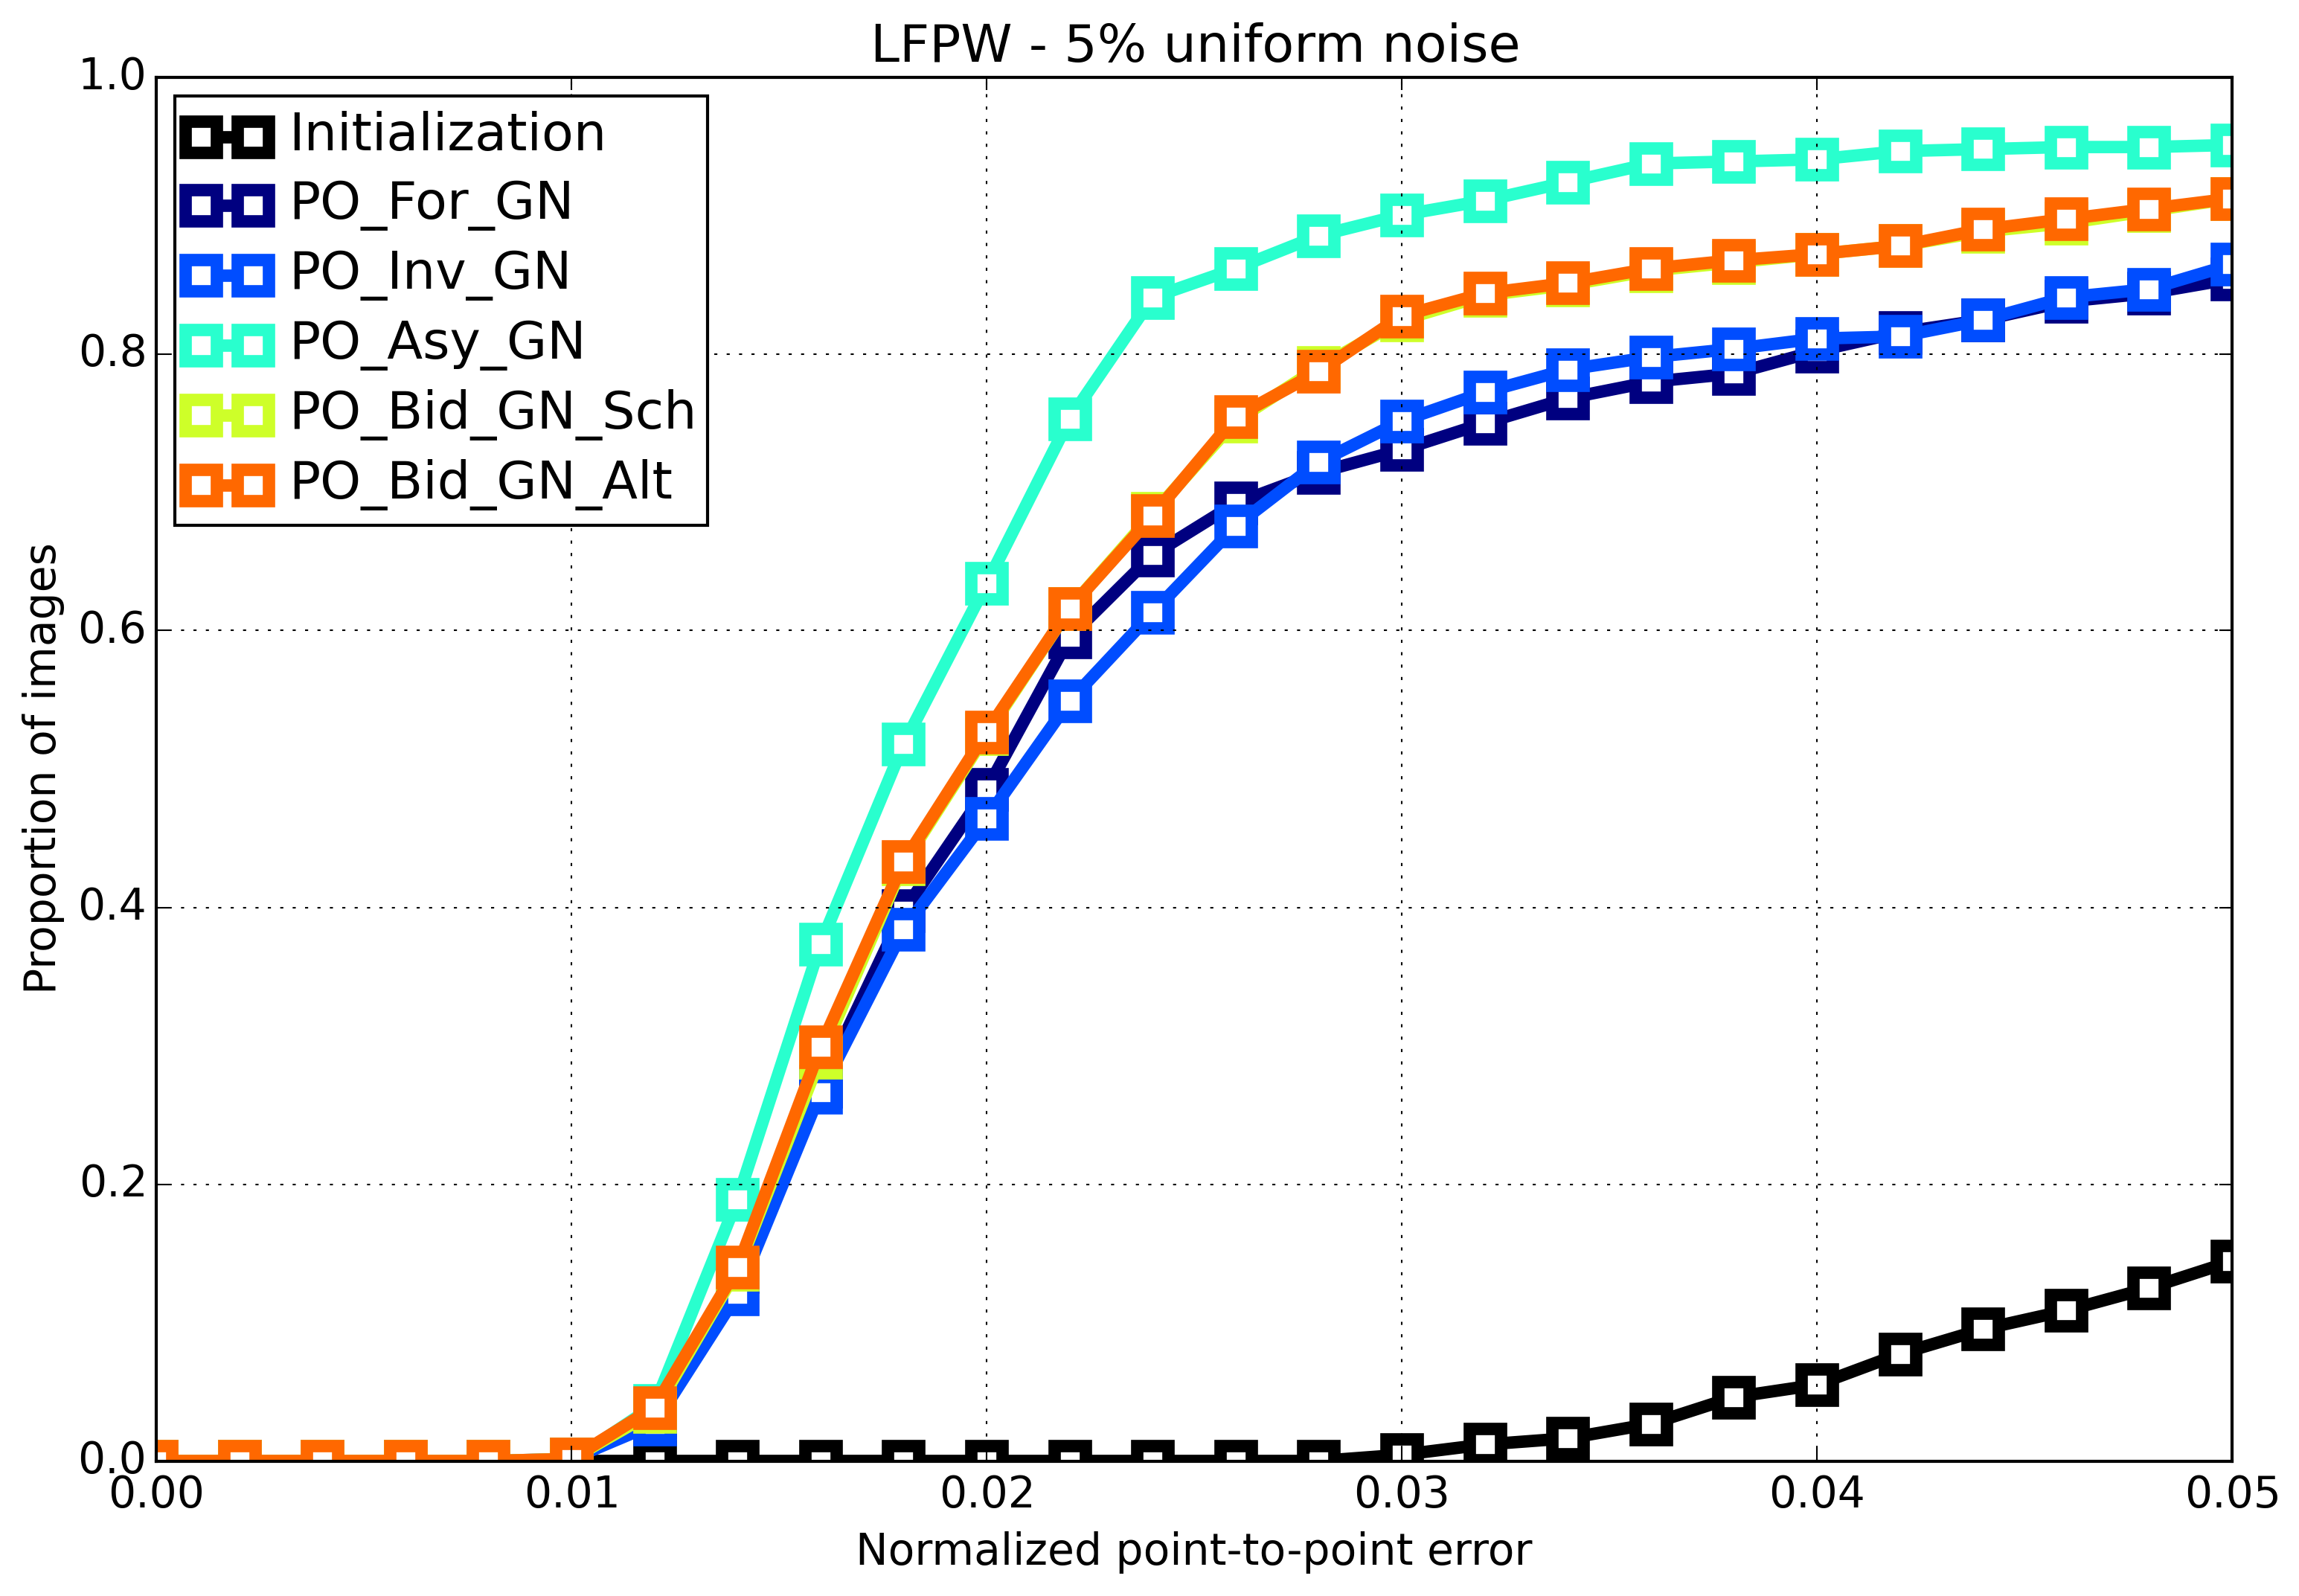
\includegraphics[width=\textwidth]{experiments/algorithms/po_gn/ced_po_gn_5.png}
	    \caption{Cumulative Error Distribution graph on the LFPW test dataset for all Project-Out Gauss-Newton algorithms initialized with $5\%$ uniform noise.}
	    \label{fig:ced_po_gn_5}
	\end{subfigure}
	\hfill
	\begin{subfigure}{0.48\textwidth}
	    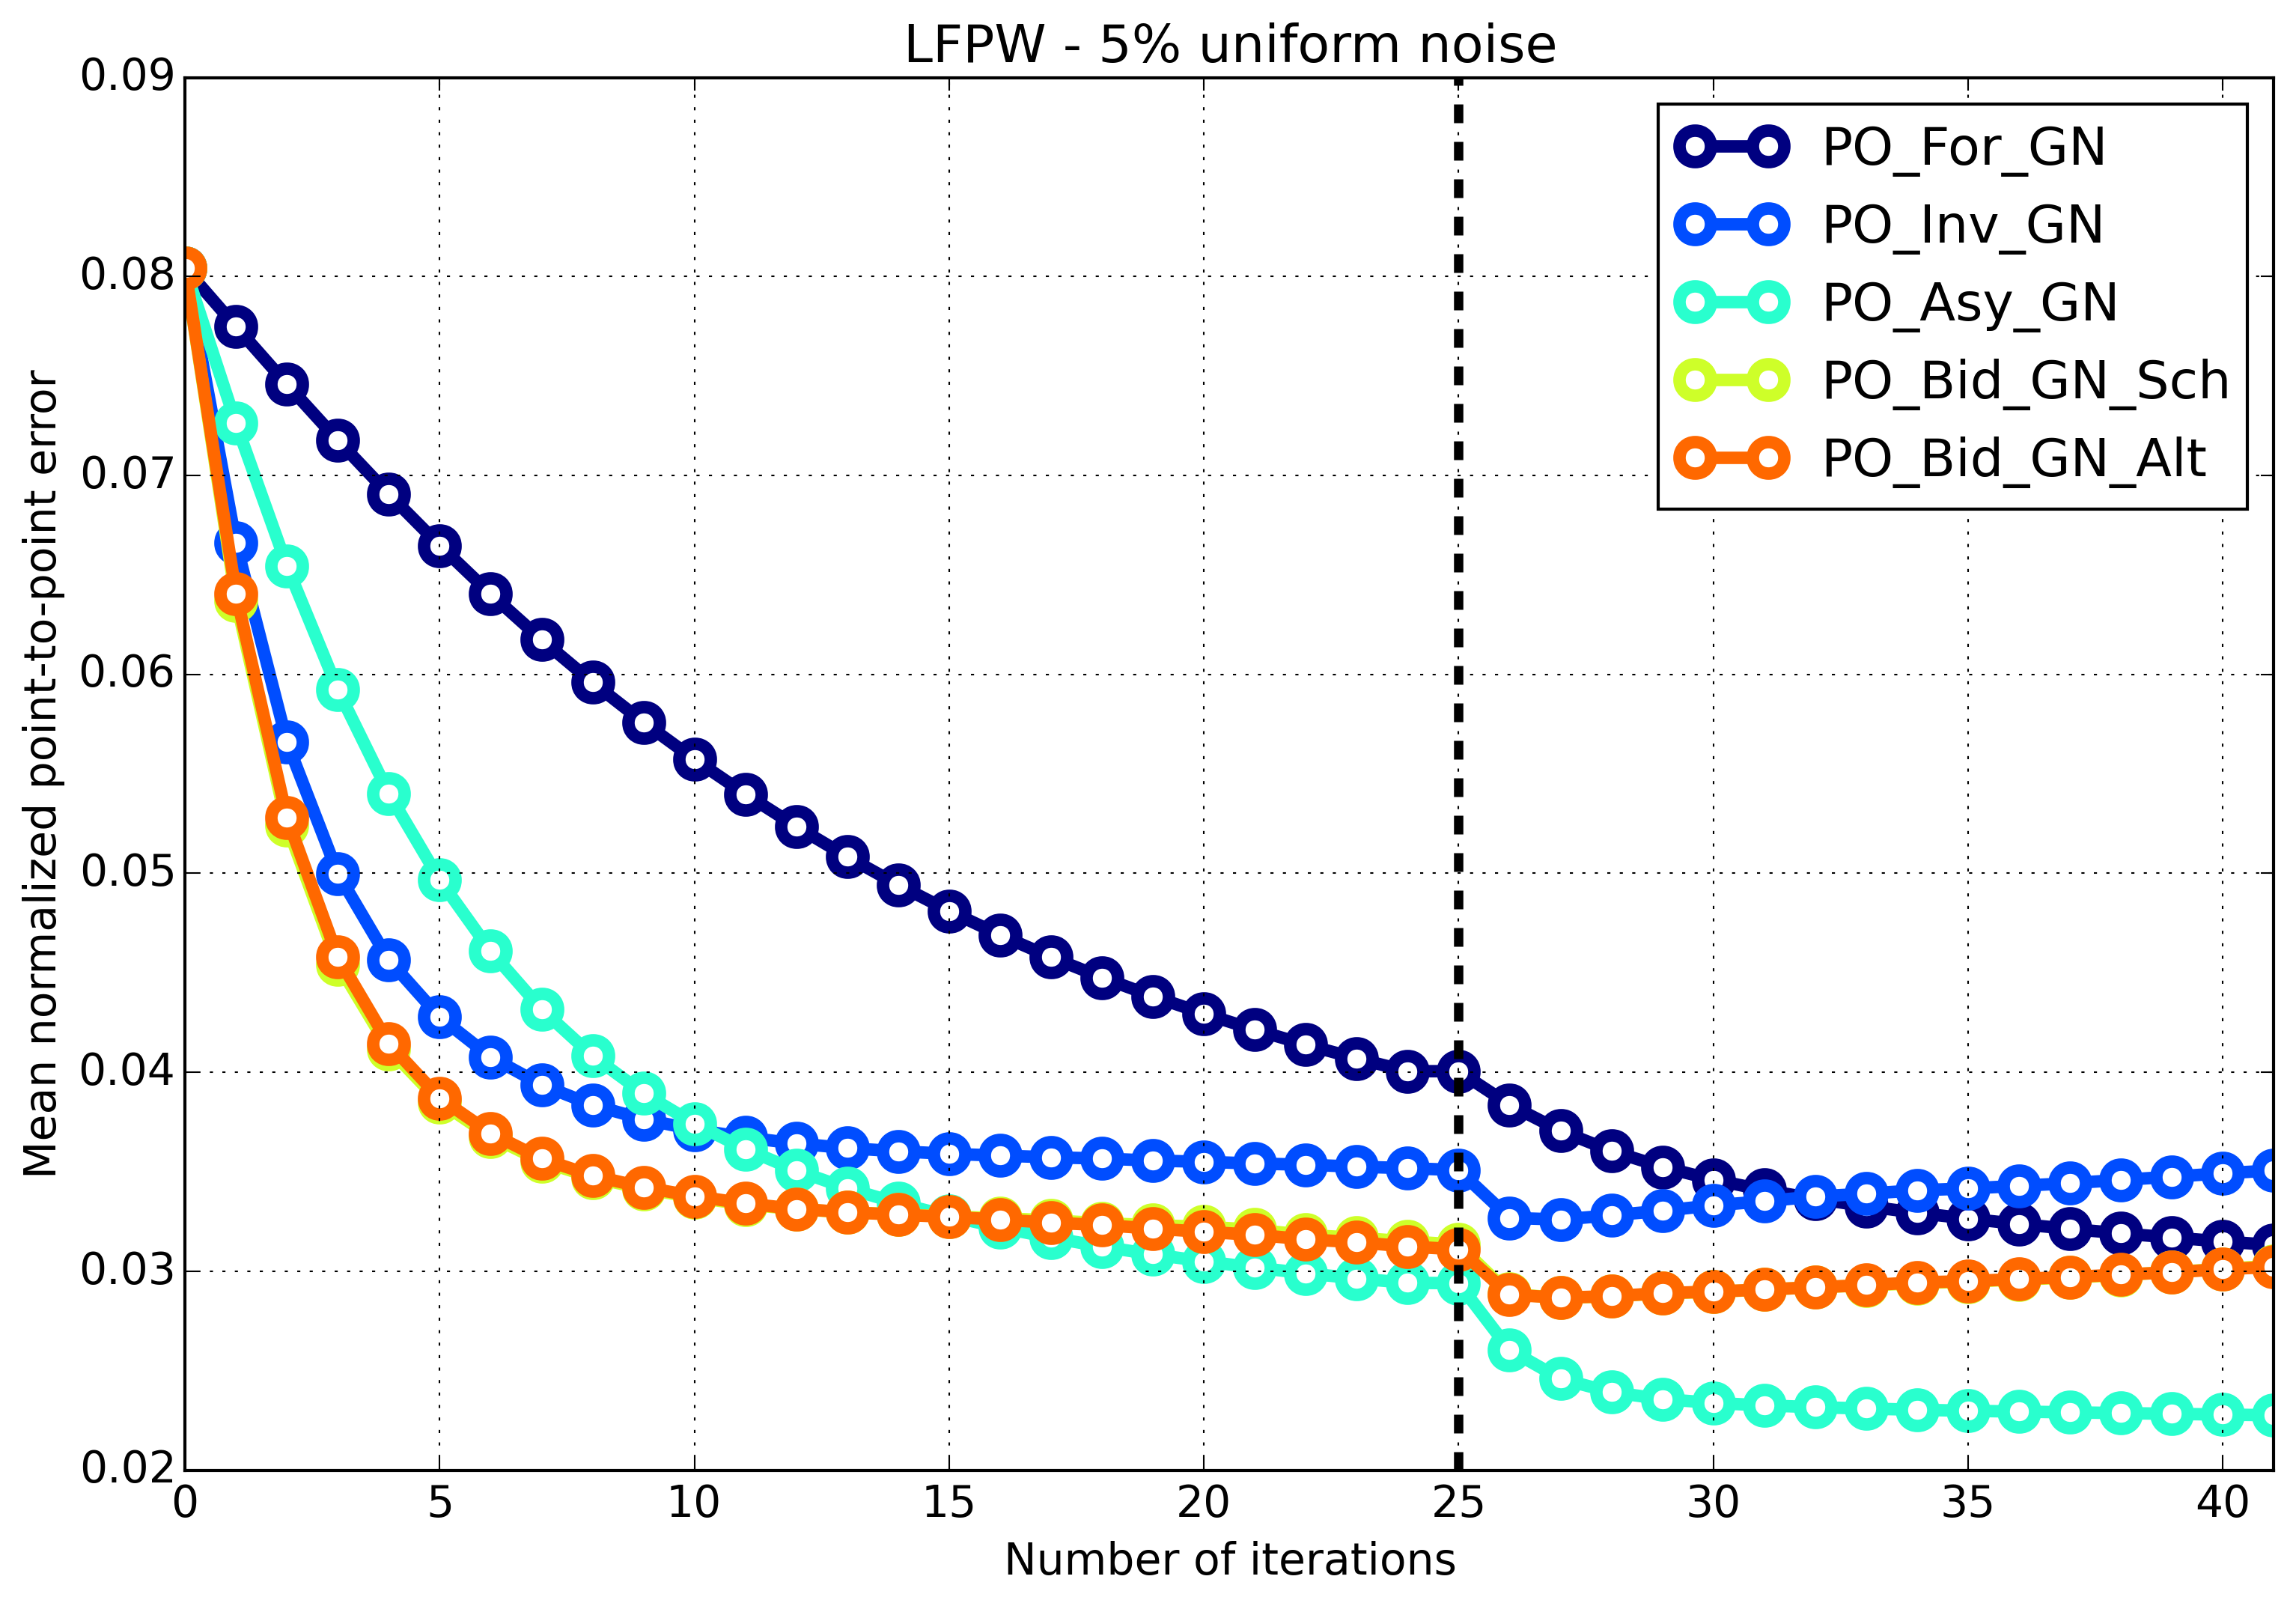
\includegraphics[width=\textwidth]{experiments/algorithms/po_gn/mean_error_vs_iters_po_gn_5.png}
	    \caption{Mean normalized point-to-point error vs number of iterations graph on the LFPW test dataset for all Project-Out Gauss-Newton algorithms initialized with $5\%$ uniform noise.}
	    \label{fig:mean_error_vs_iters_po_gn_5}
	\end{subfigure}
	\par\medskip
	\begin{subfigure}{0.48\textwidth}
	    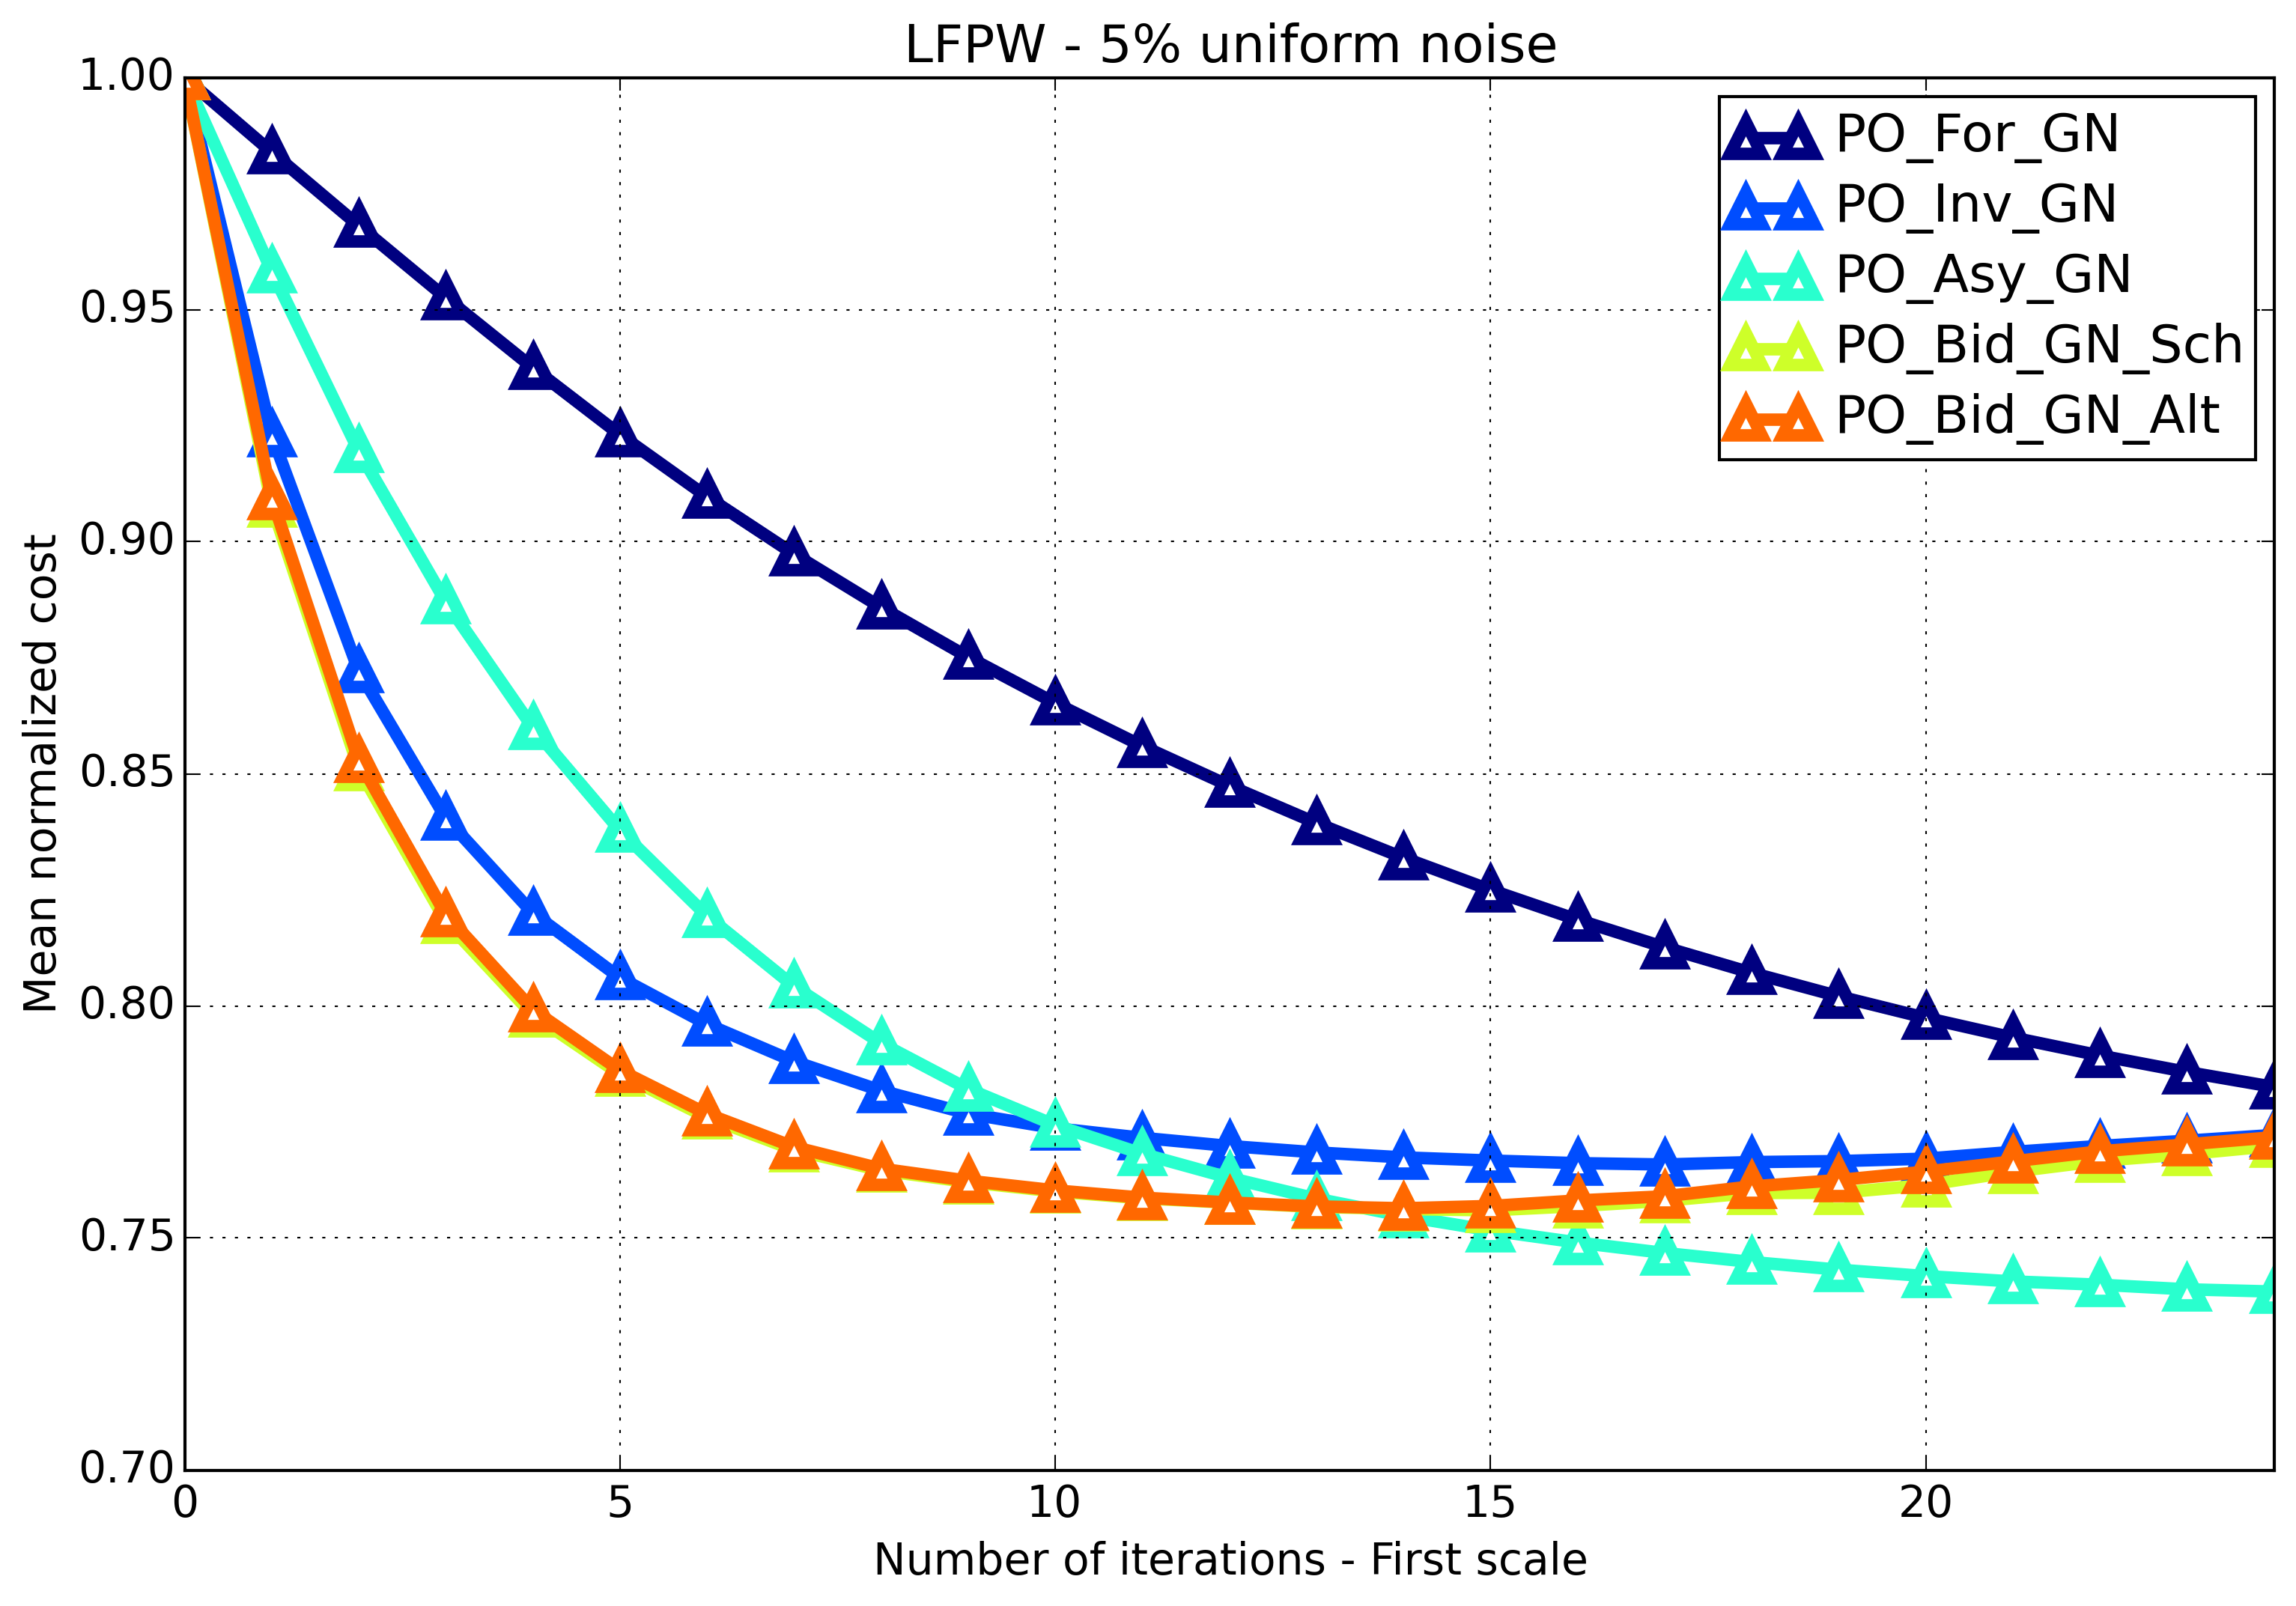
\includegraphics[width=\textwidth]{experiments/algorithms/po_gn/mean_cost_vs_iters1_po_gn_5.png}
	    \caption{Mean normalized cost vs number of first scale iterations graph on the LFPW test dataset for all Project-Out Gauss-Newton algorithms initialized with $5\%$ uniform noise.}
	    \label{fig:mean_cost_vs_iters1_po_gn_5}
	\end{subfigure}
	\hfill
	\begin{subfigure}{0.48\textwidth}
	    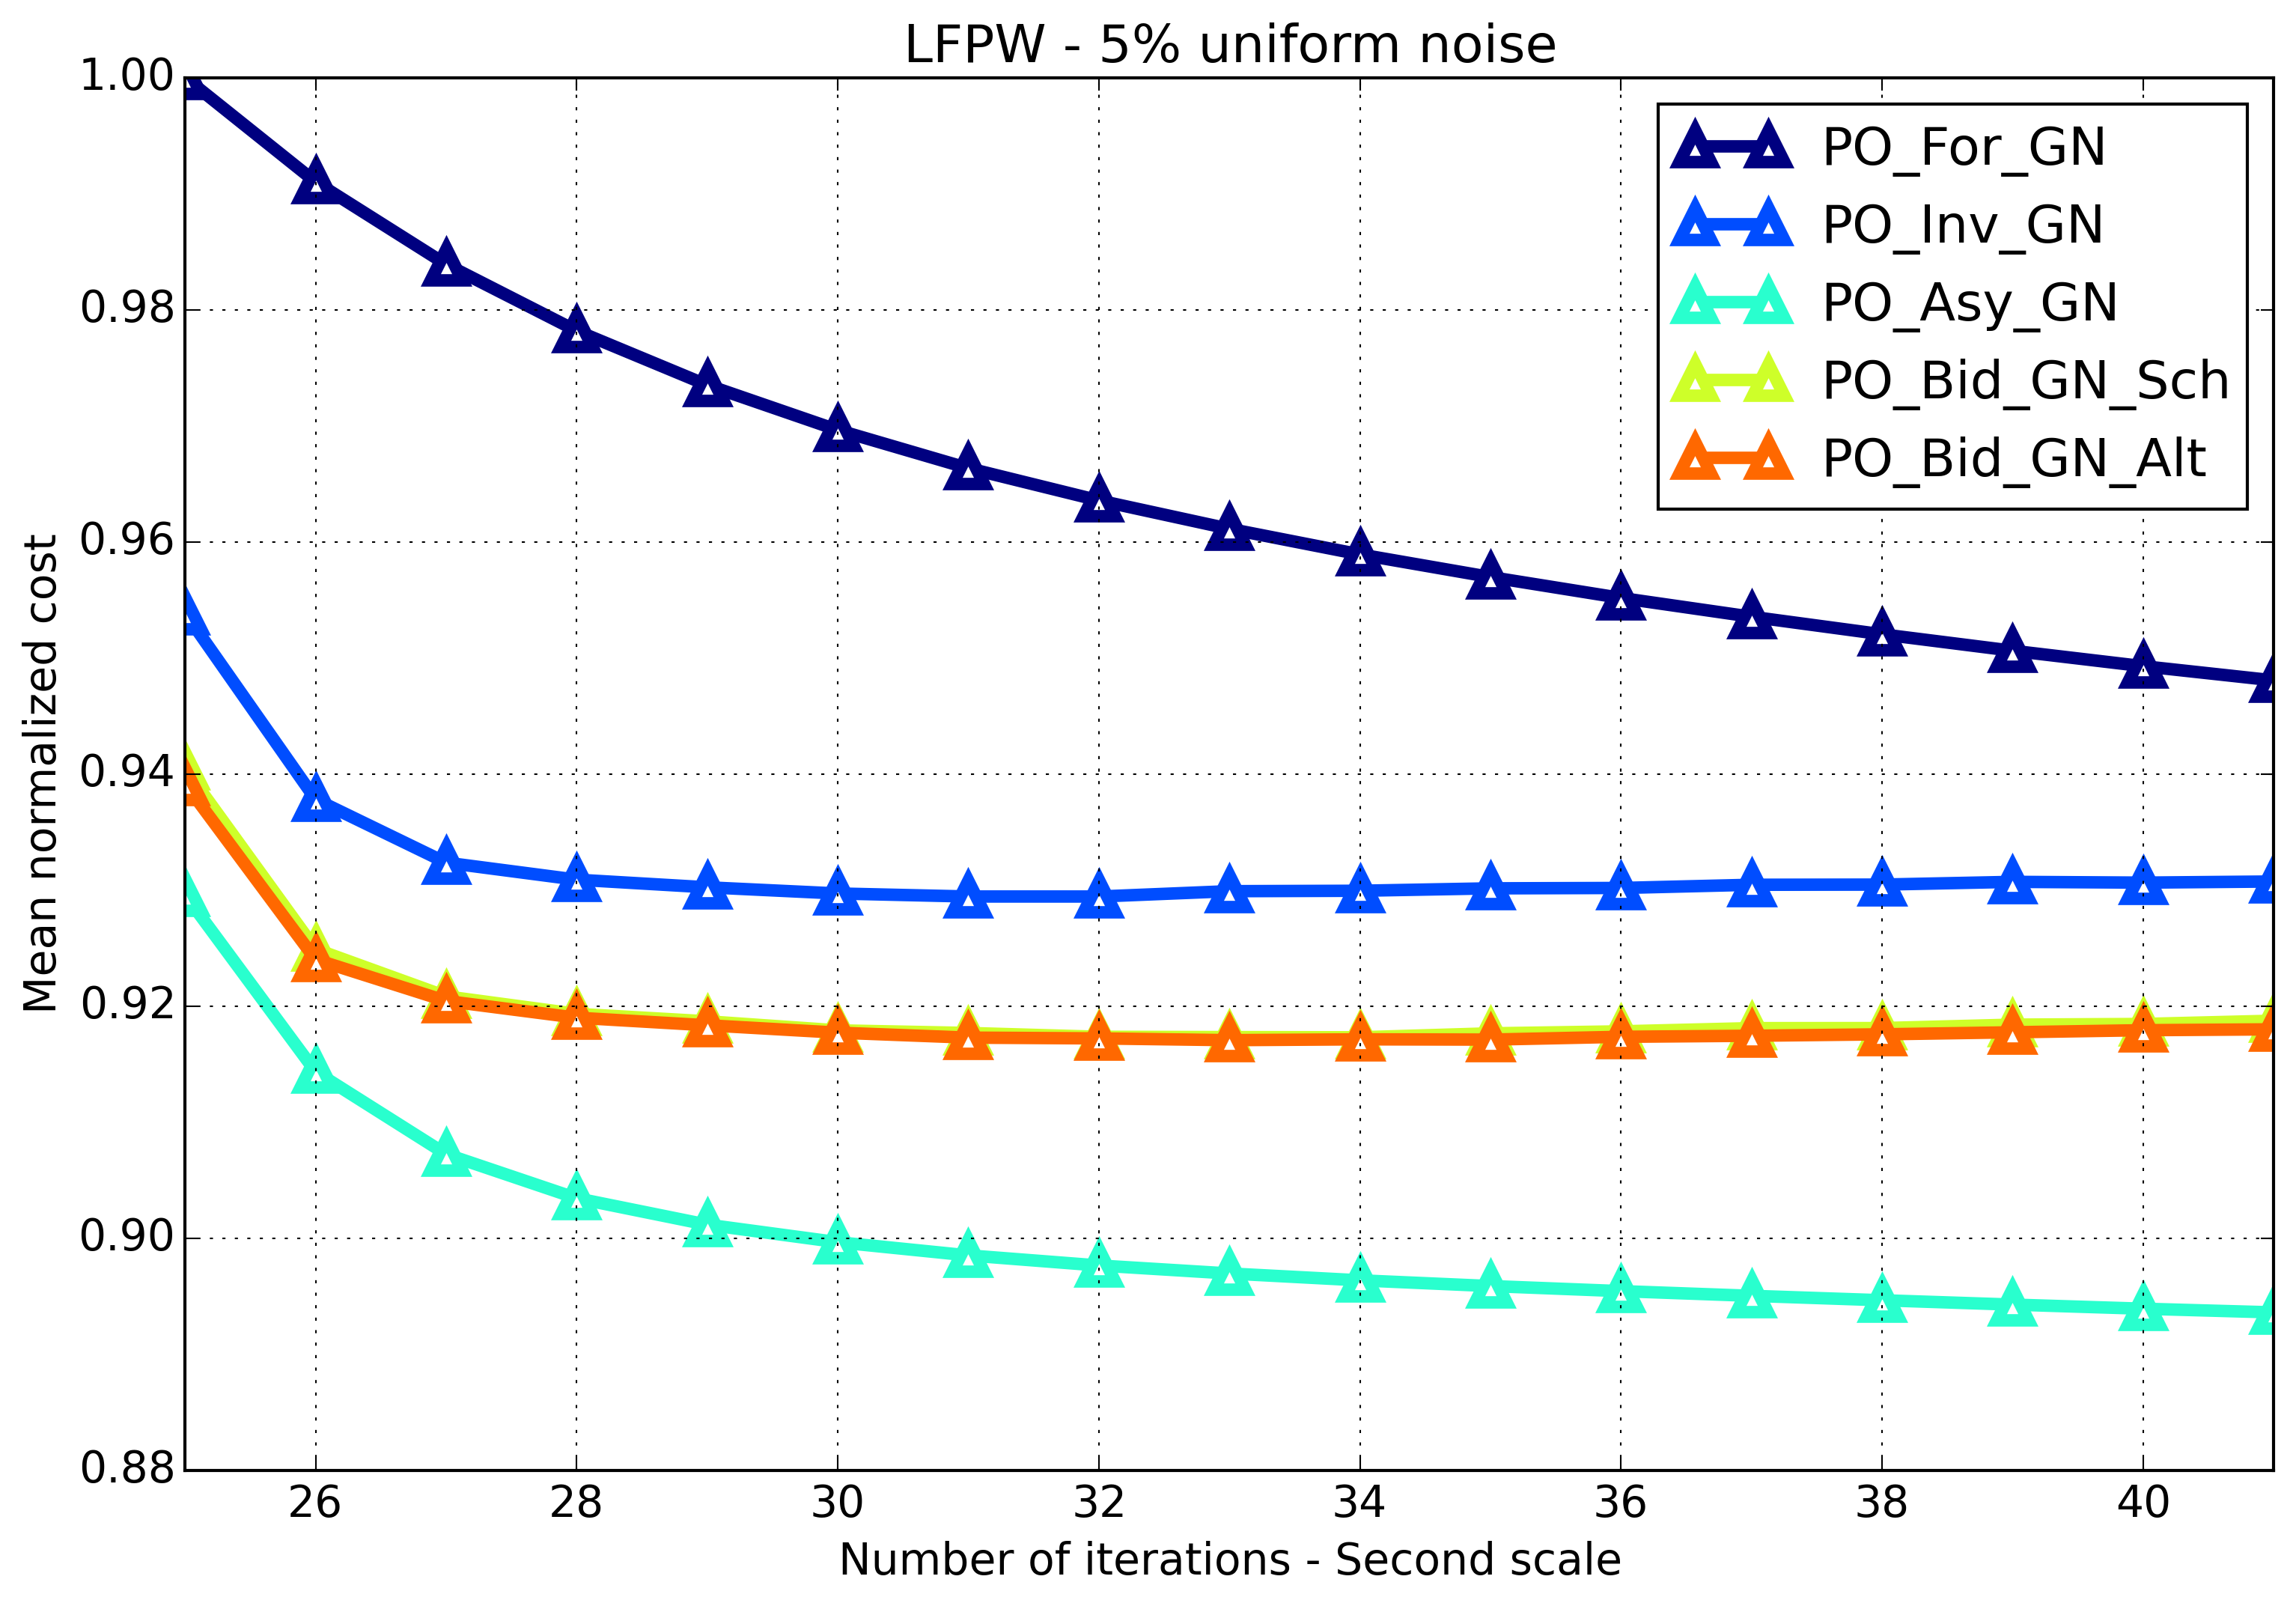
\includegraphics[width=\textwidth]{experiments/algorithms/po_gn/mean_cost_vs_iters2_po_gn_5.png}
	    \caption{Mean normalized cost vs number of second scale iterations graph on the LFPW test dataset for all Project-Out Gauss-Newton algorithms initialized with $5\%$ uniform noise.}
	    \label{fig:mean_cost_vs_iters2_po_gn_5}
	\end{subfigure}
	\label{fig:po_gn_5}
	\caption{}
\end{figure*}


% \subsubsection{Project-Out Newton algorithms}

% \begin{figure}[h!]
%     \centering
%     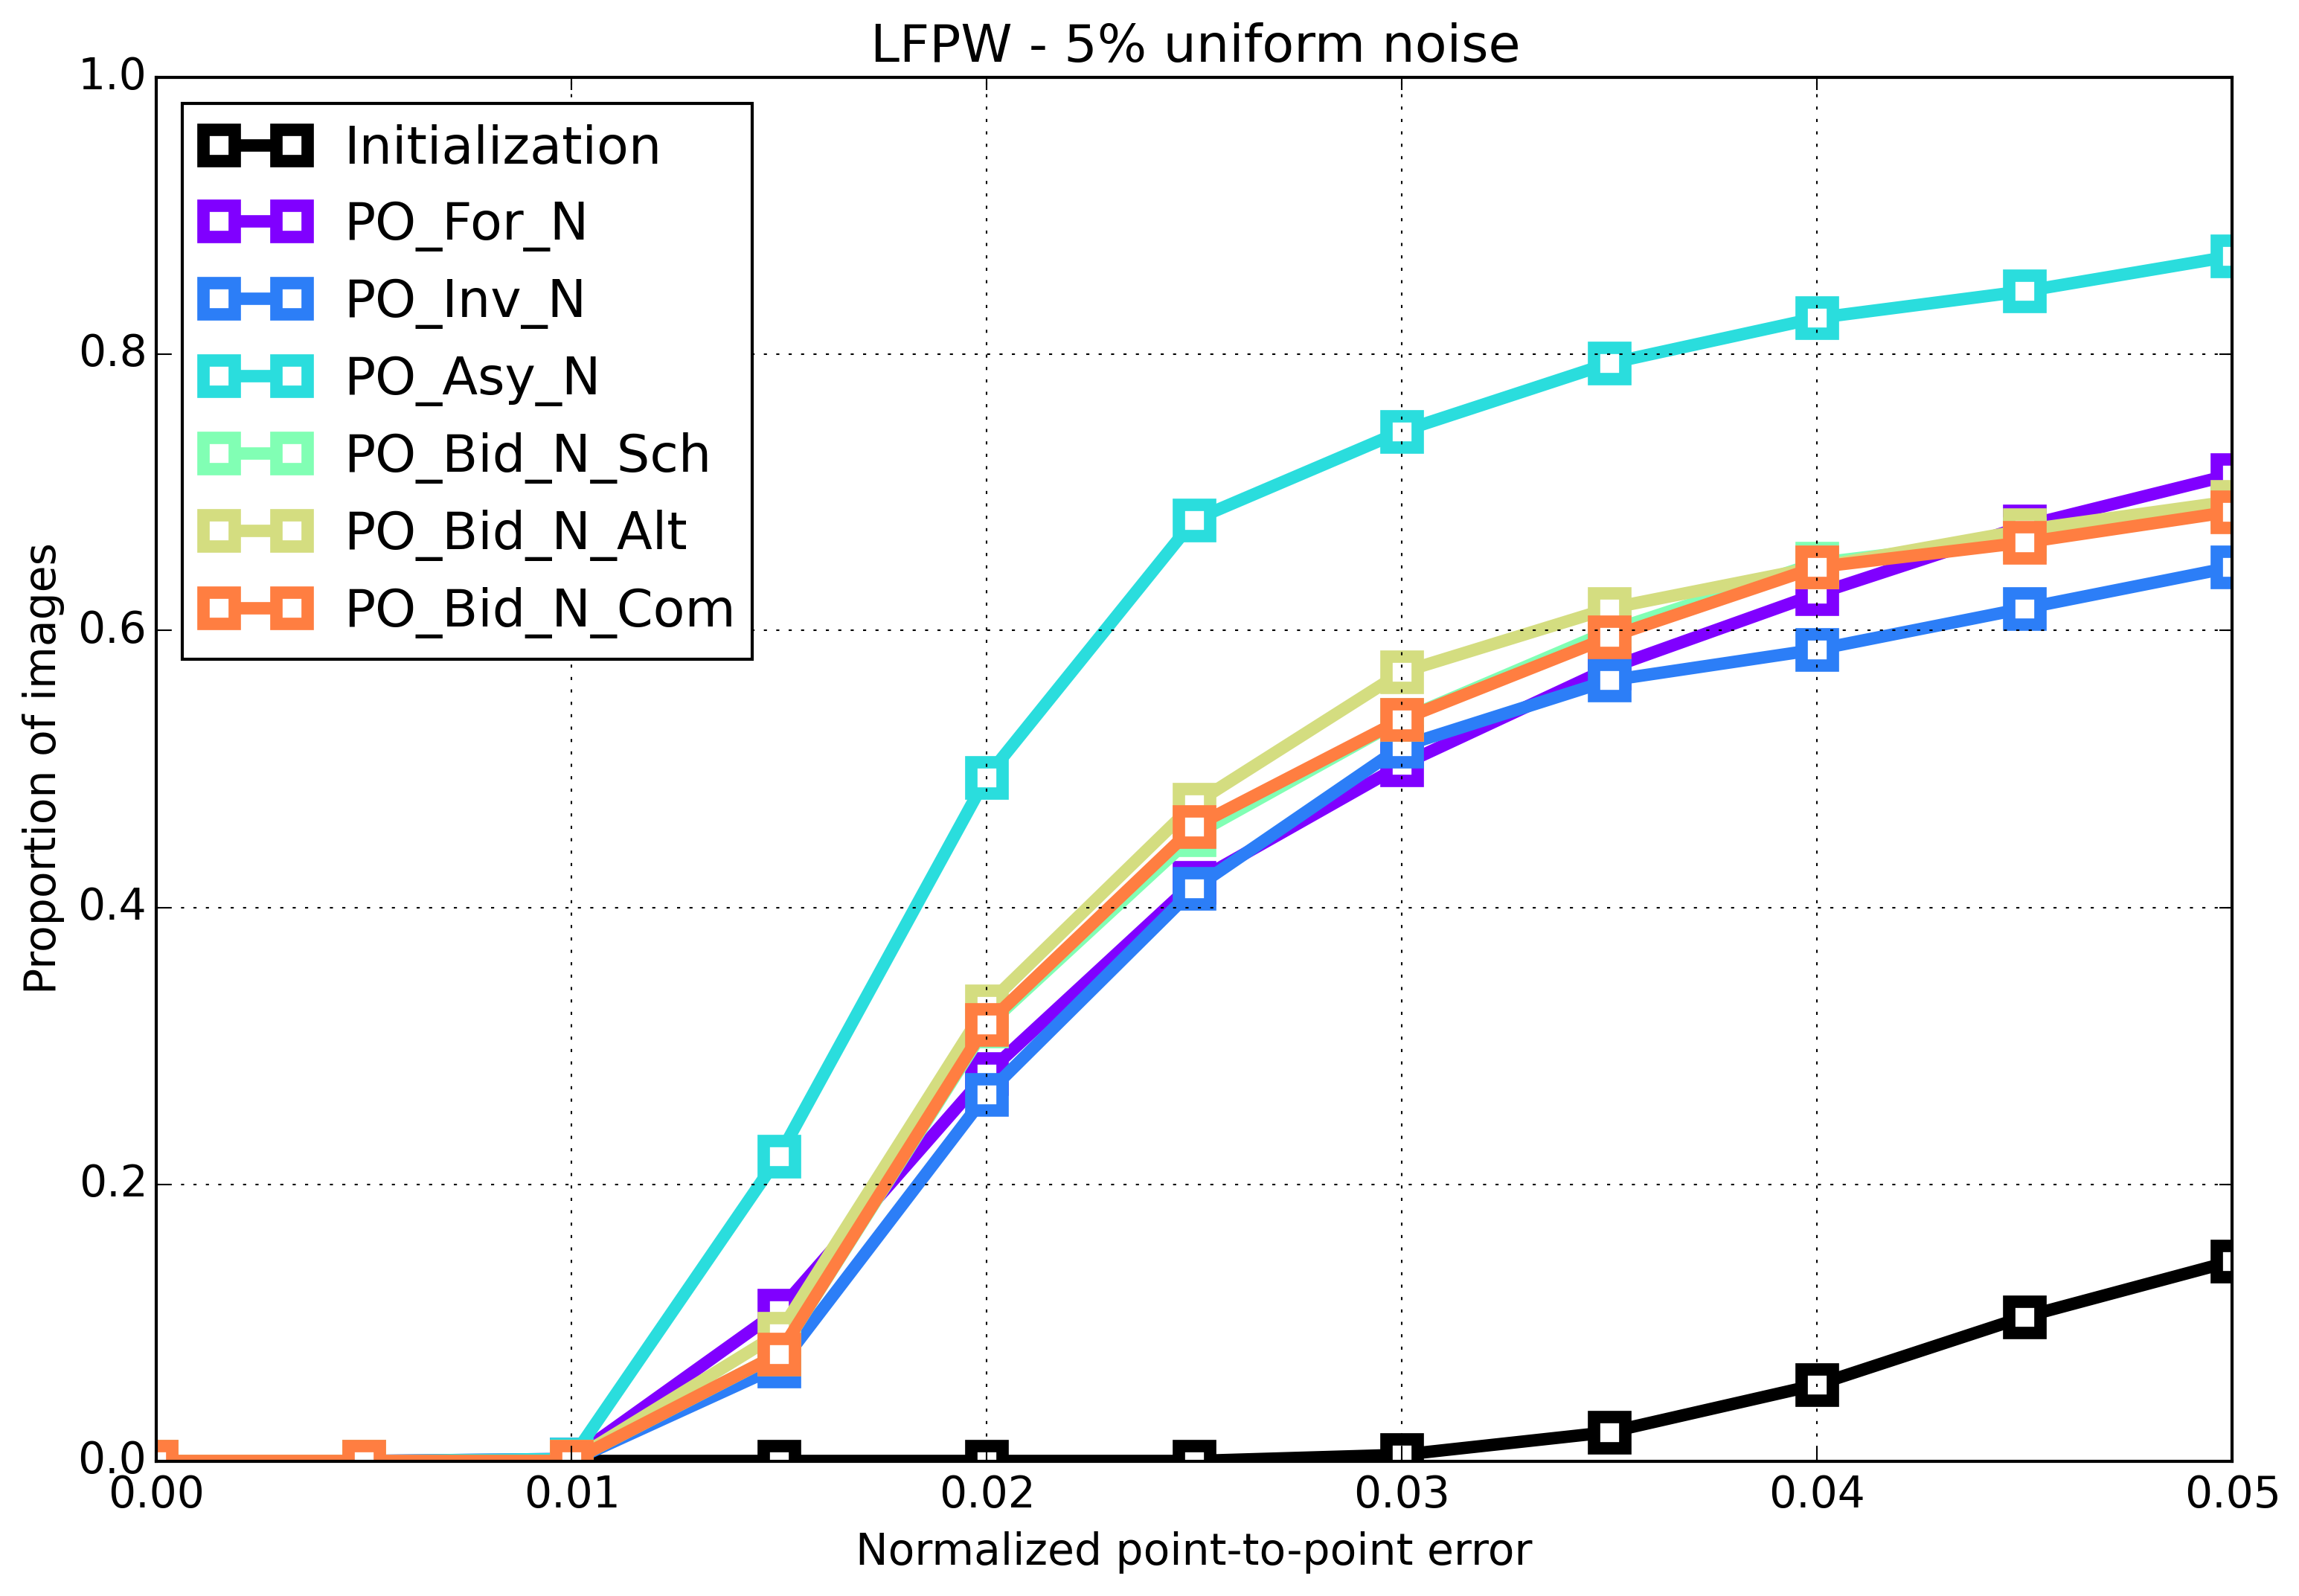
\includegraphics[width=0.50\textwidth]{experiments/algorithms/po_n/ced_po_n_5.png}
%     \caption{CED graph on the LFPW test dataset for all Project-Out Newton algorithms initialized with $4$\% uniform noise.}
%     \label{fig:ced_po_gn_4}
% \end{figure}

% \begin{figure}[h!]
%     \centering
%     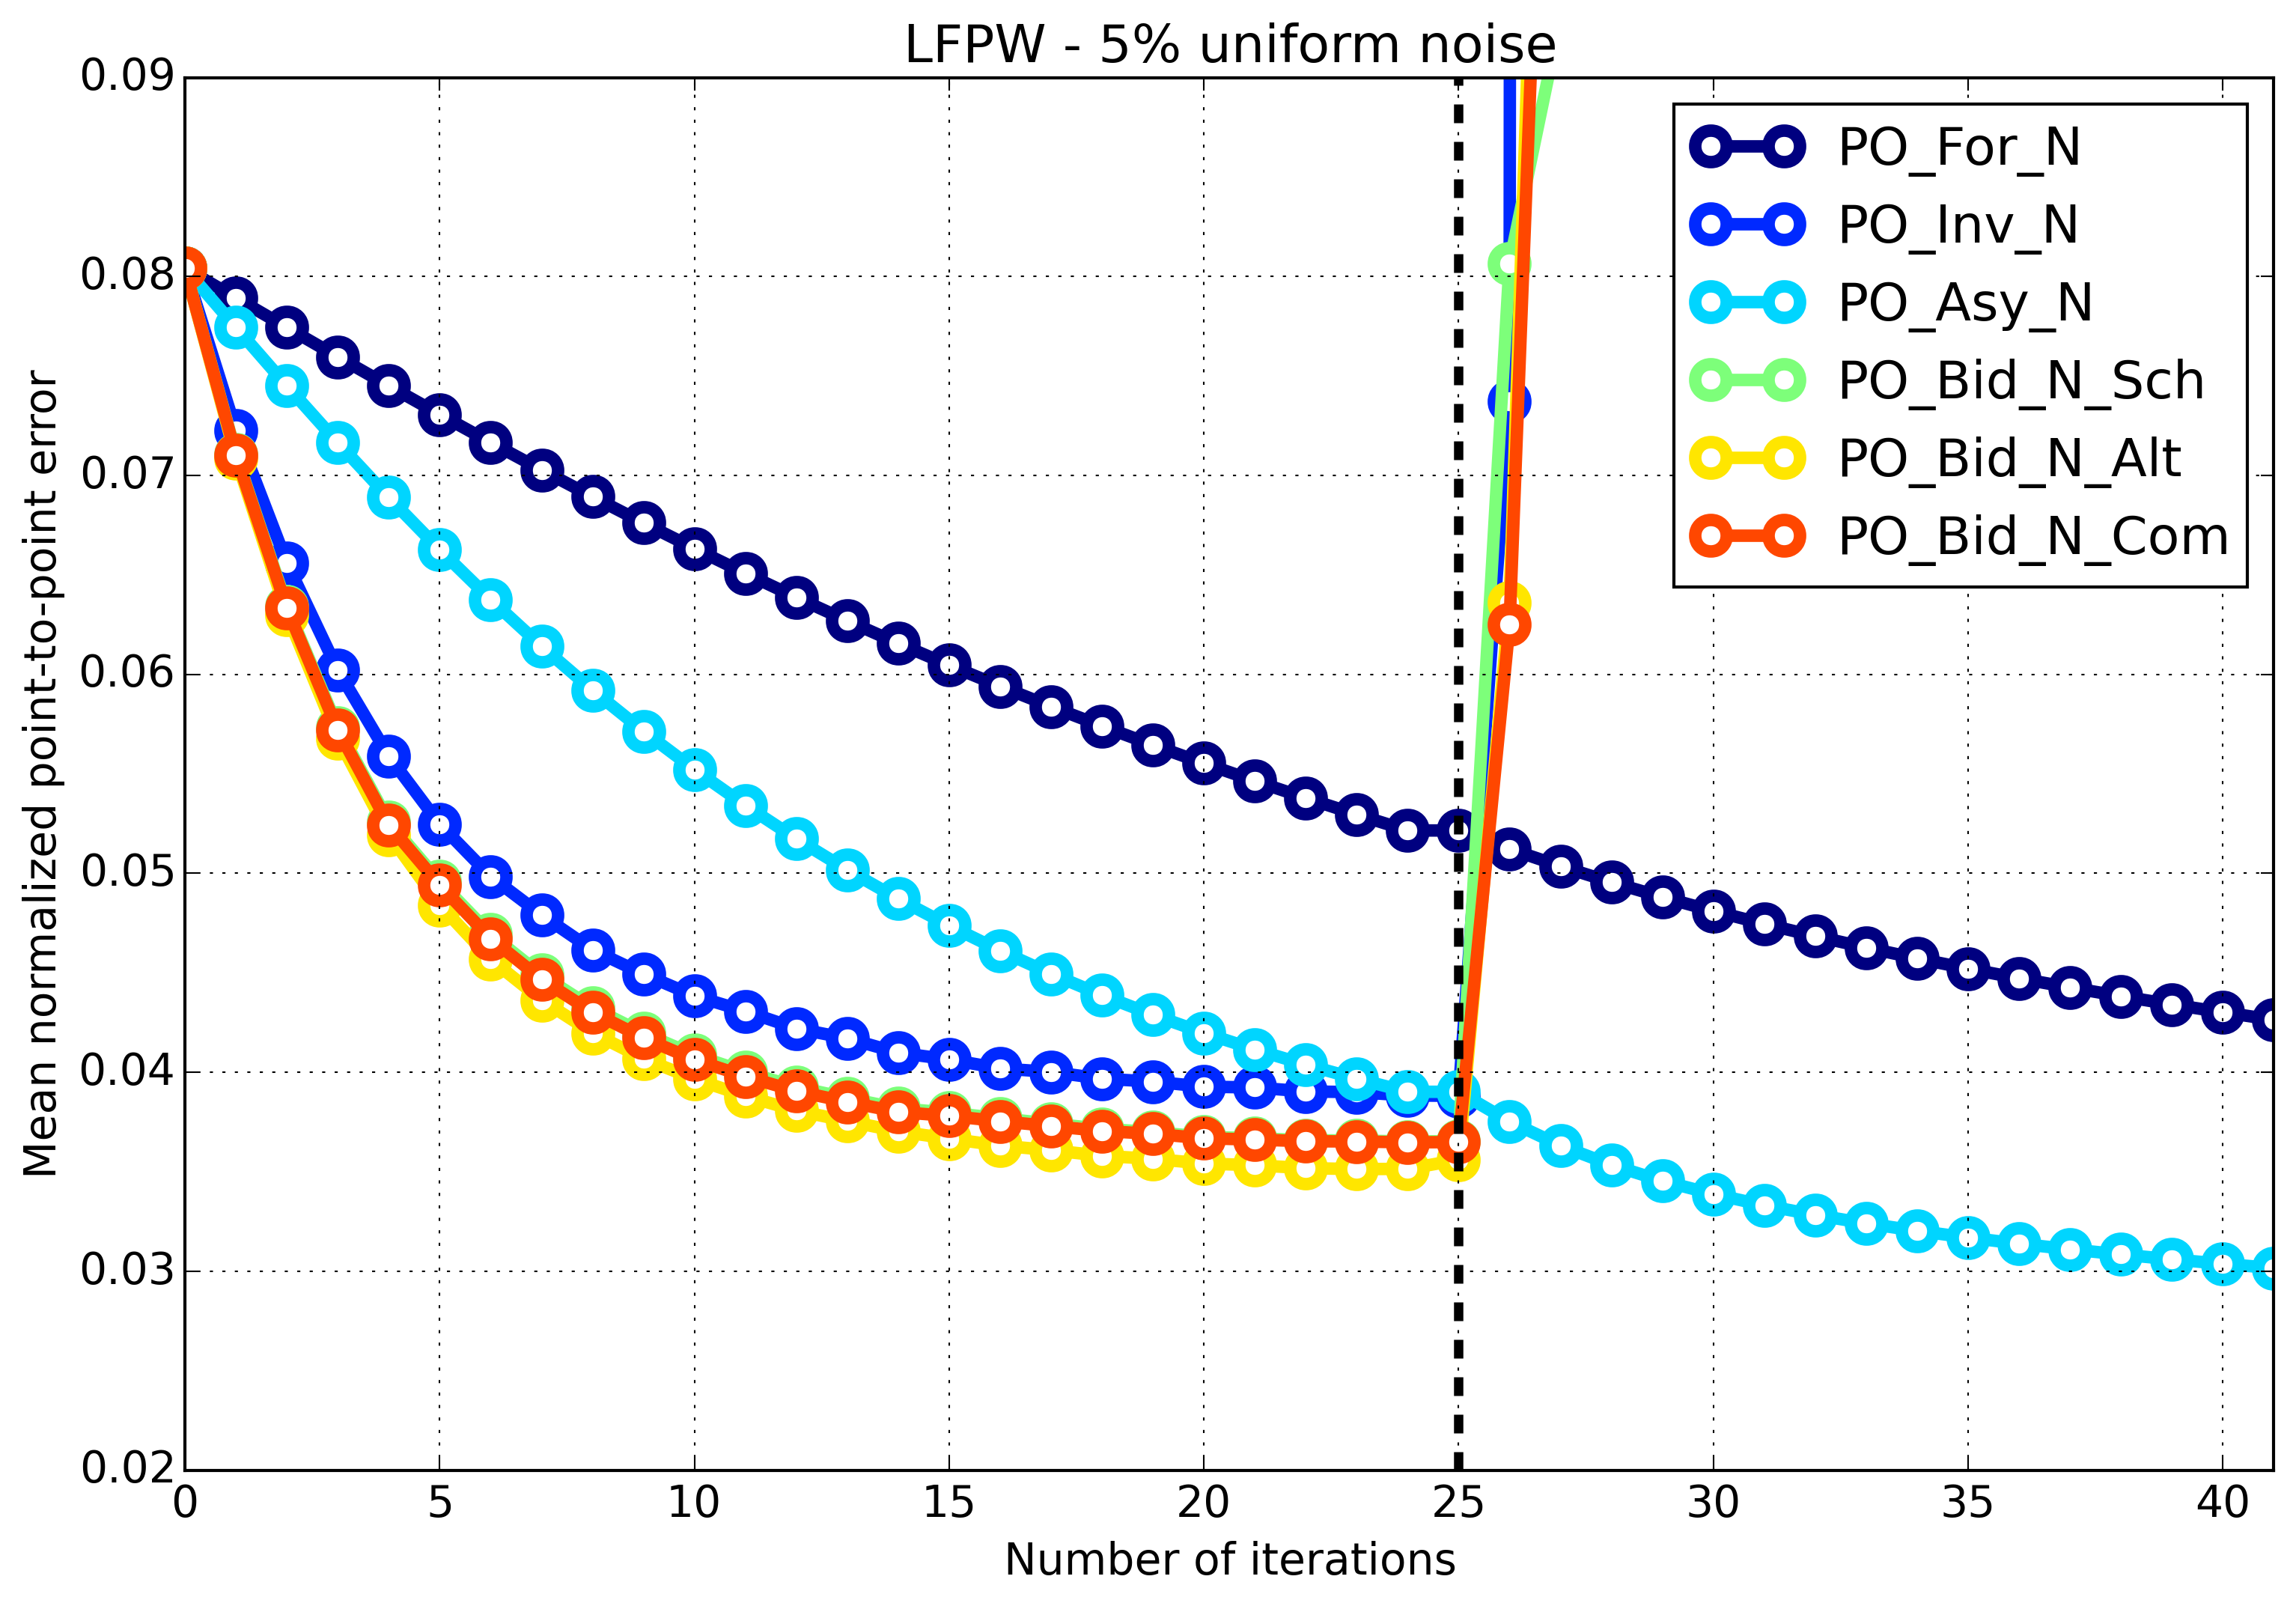
\includegraphics[width=0.50\textwidth]{experiments/algorithms/po_n/mean_error_vs_iters_po_n_5.png}
%     \caption{Mean normalized point-to-point error vs number of iterations graph on the LFPW test dataset for all Project-Out Newton algorithms initialized with $4$\% uniform noise.}
%     \label{fig:mean_error_vs_iters_po_n_4}
% \end{figure}

% \begin{figure}[h!]
%     \centering
%     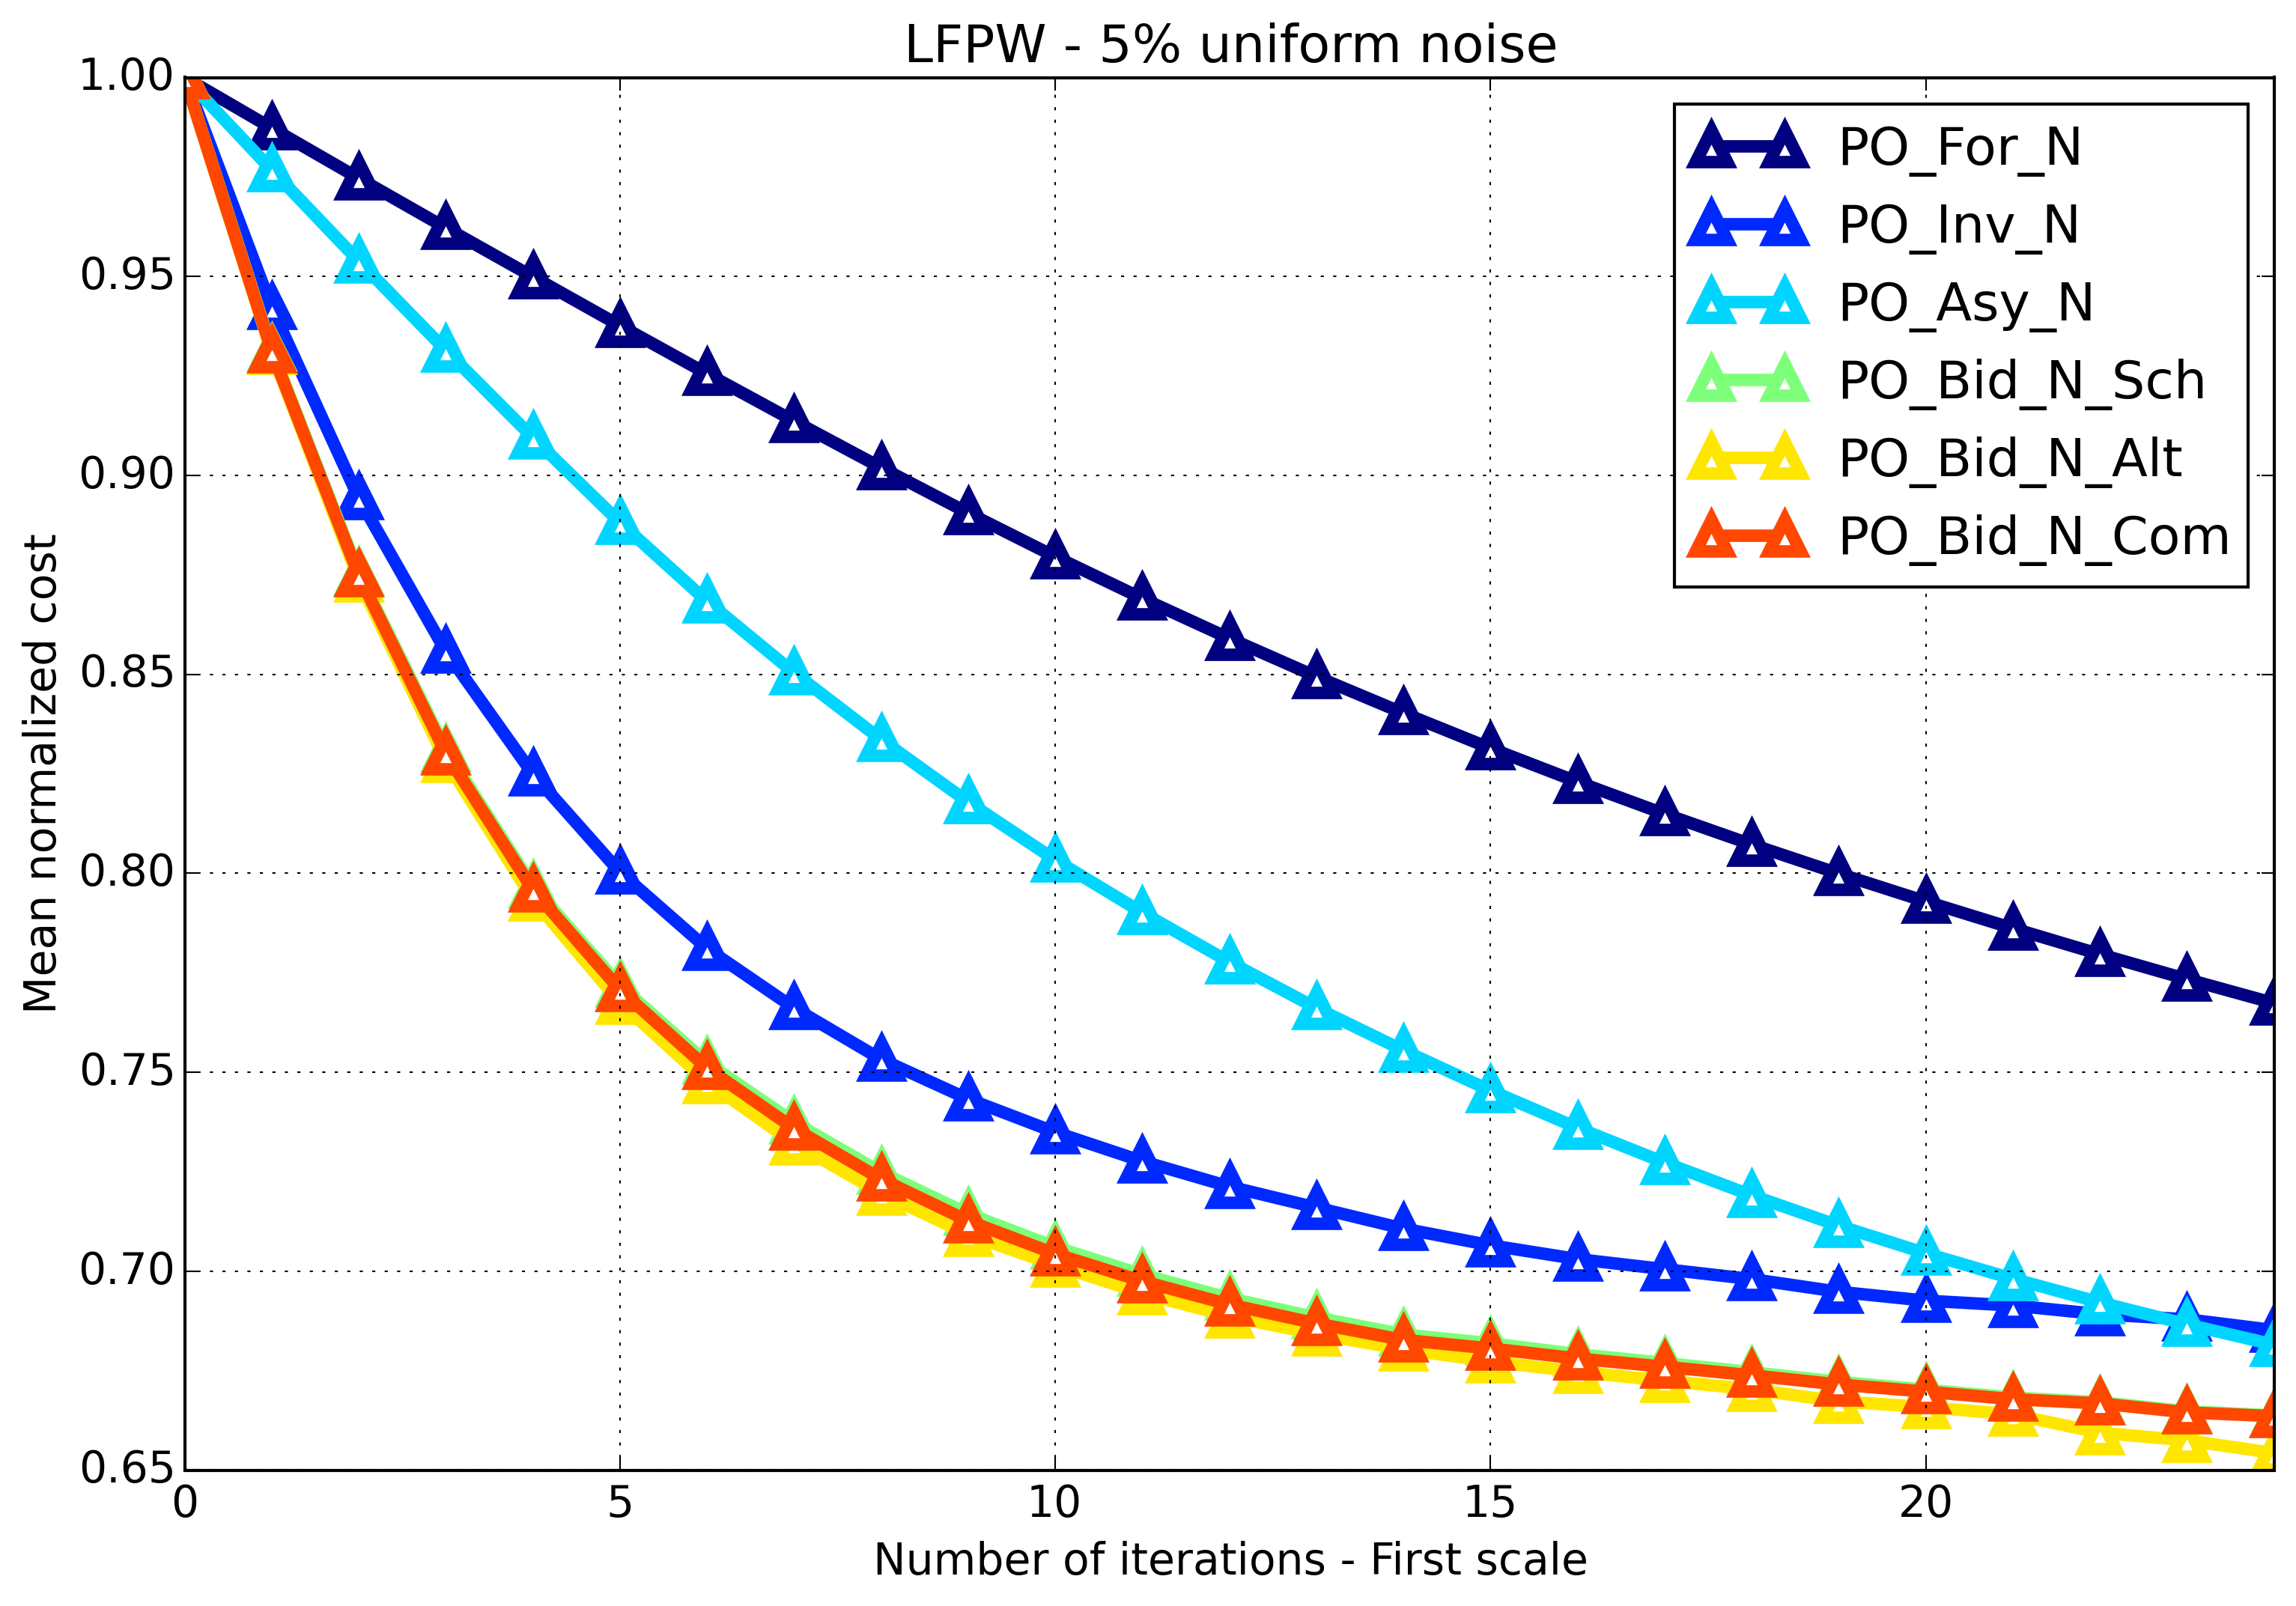
\includegraphics[width=0.50\textwidth]{experiments/algorithms/po_n/mean_cost_vs_iters1_po_n_5.png}
%     \caption{Mean normalized cost vs number of first scale iterations graph on the LFPW test dataset for all Project-Out Newton algorithms initialized with $4$\% uniform noise.}
%     \label{fig:mean_cost_vs_iters1_po_n_4}
% \end{figure}

% \begin{figure}[h!]
%     \centering
%     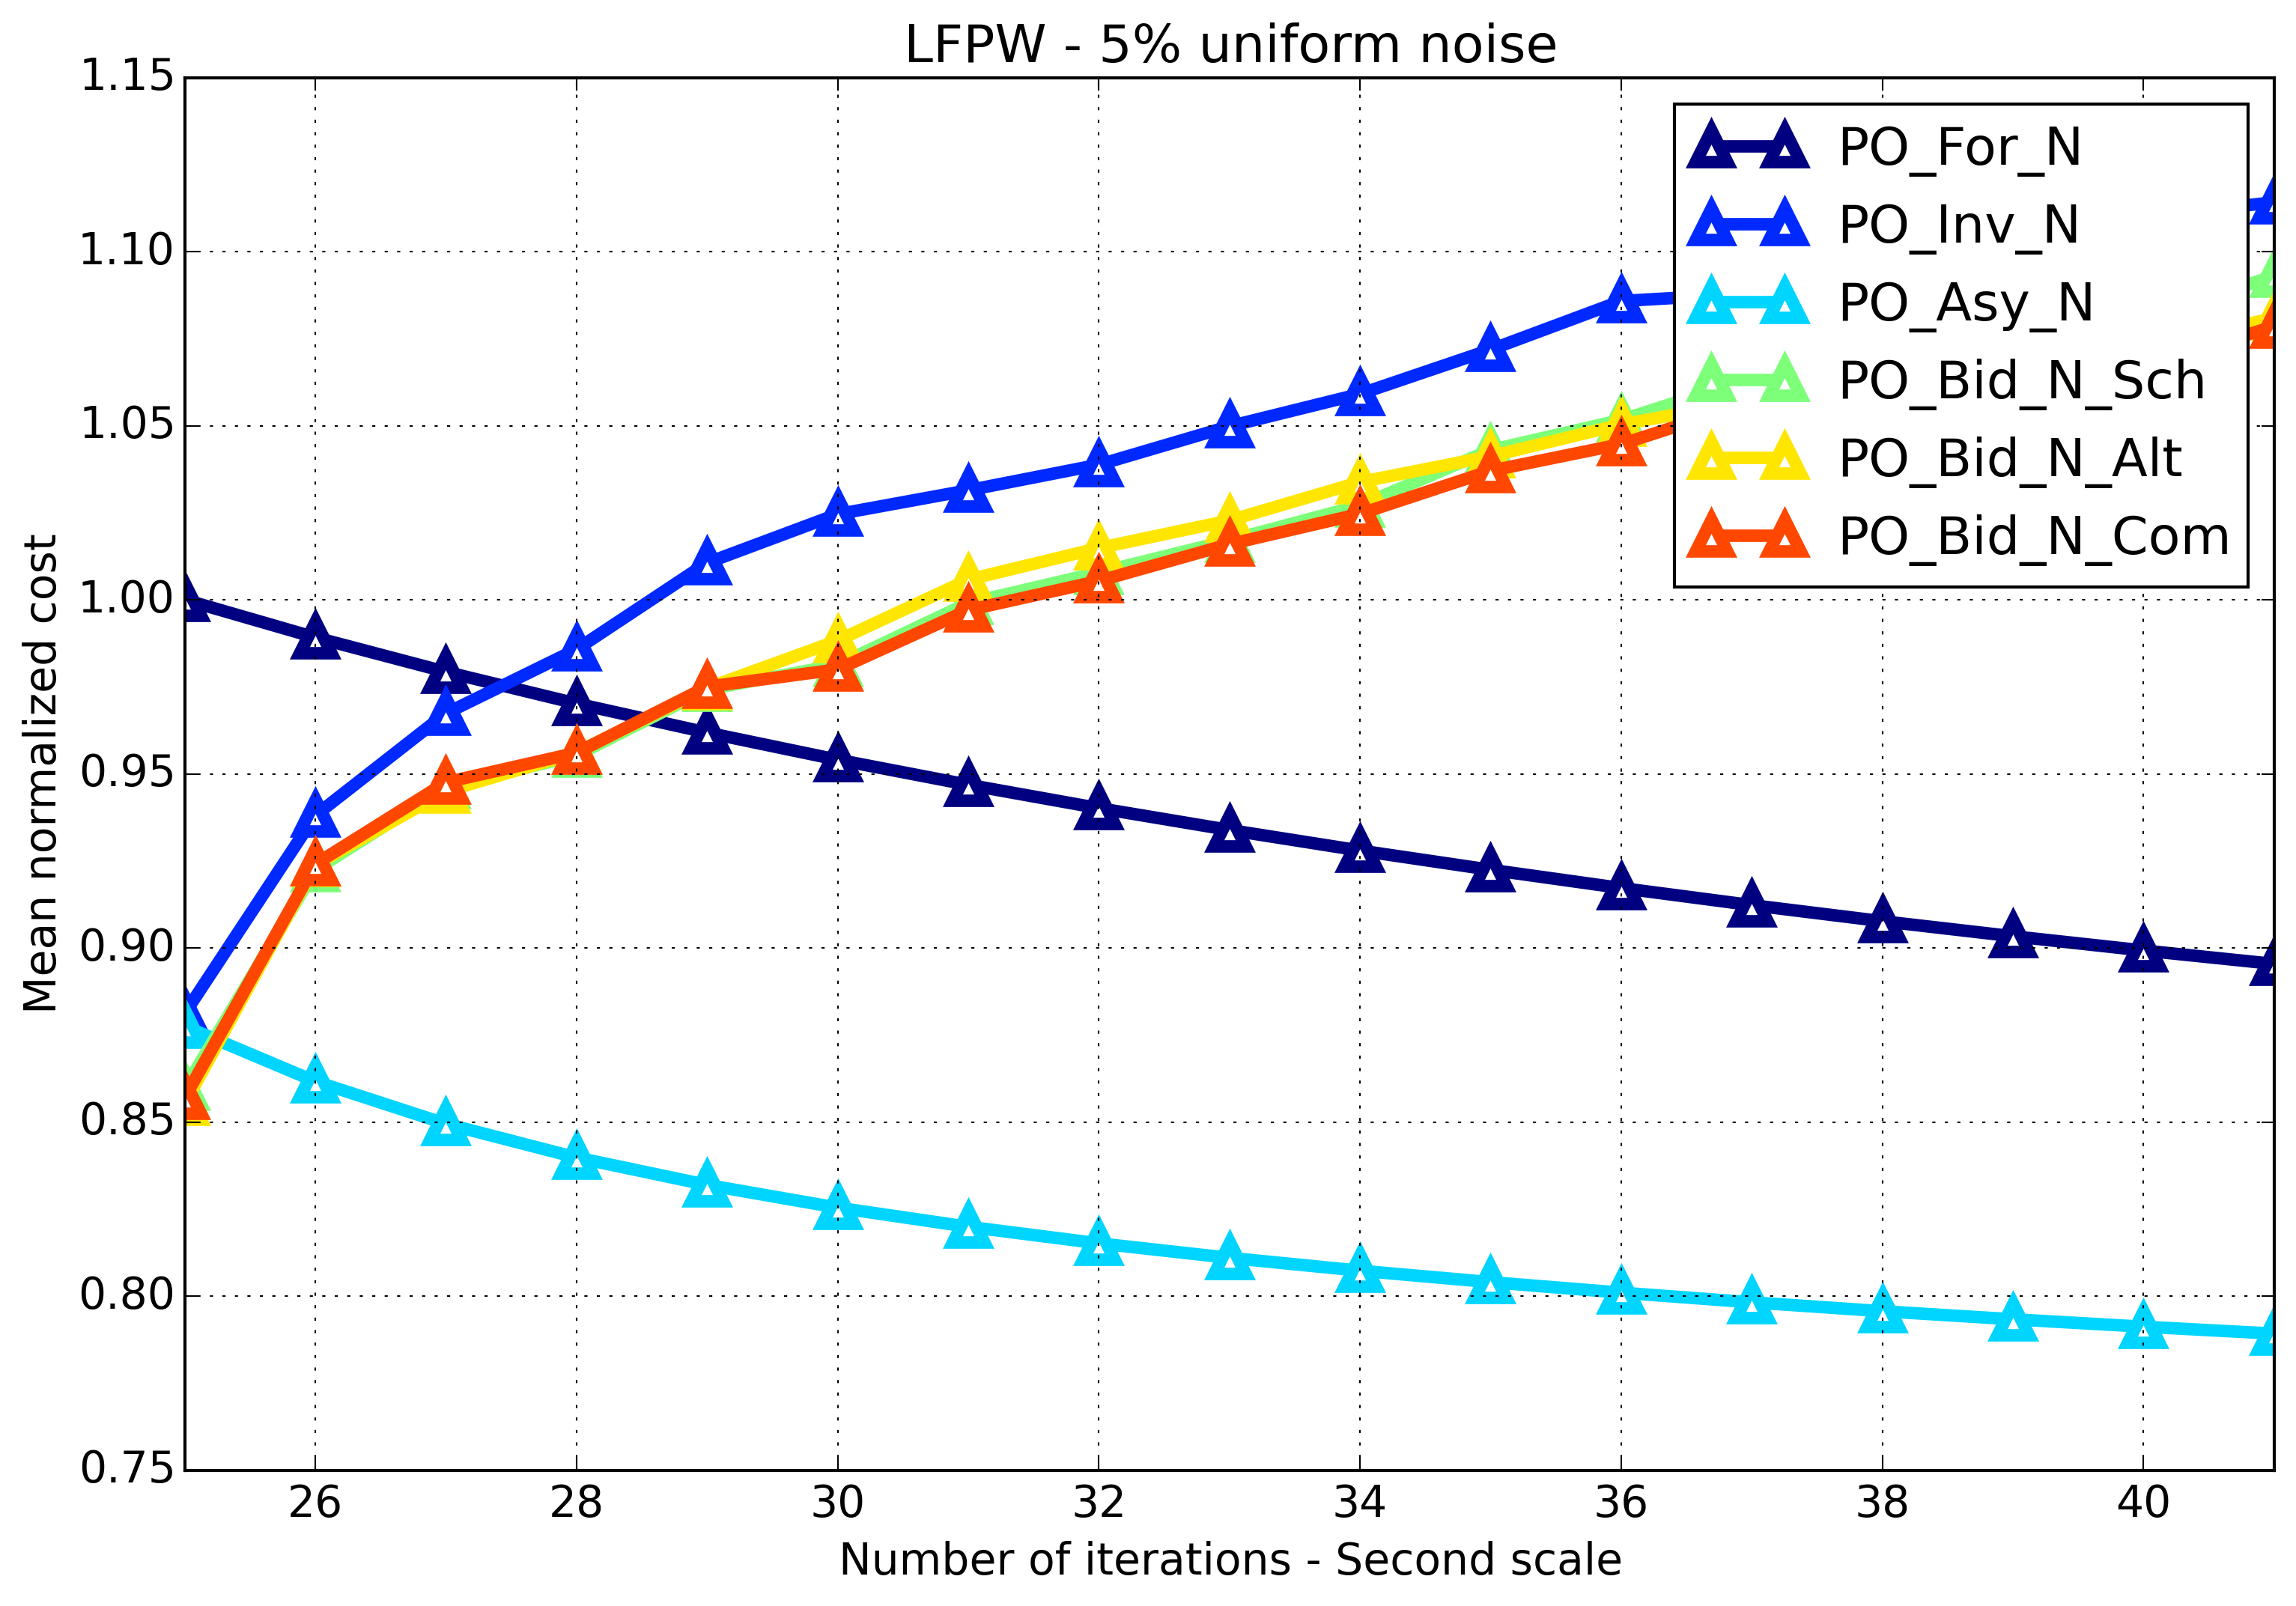
\includegraphics[width=0.50\textwidth]{experiments/algorithms/po_n/mean_cost_vs_iters2_po_n_5.png}
%     \caption{Mean normalized cost vs number of second scale iterations graph on the LFPW test dataset for all Project-Out Newton algorithms initialized with $4$\% uniform noise.}
%     \label{fig:mean_cost_vs_iters2_po_n_4}
% \end{figure}

\subsubsection*{Wiberg}

\begin{figure*}[h!]
	\centering
	\begin{subfigure}{0.48\textwidth}
	    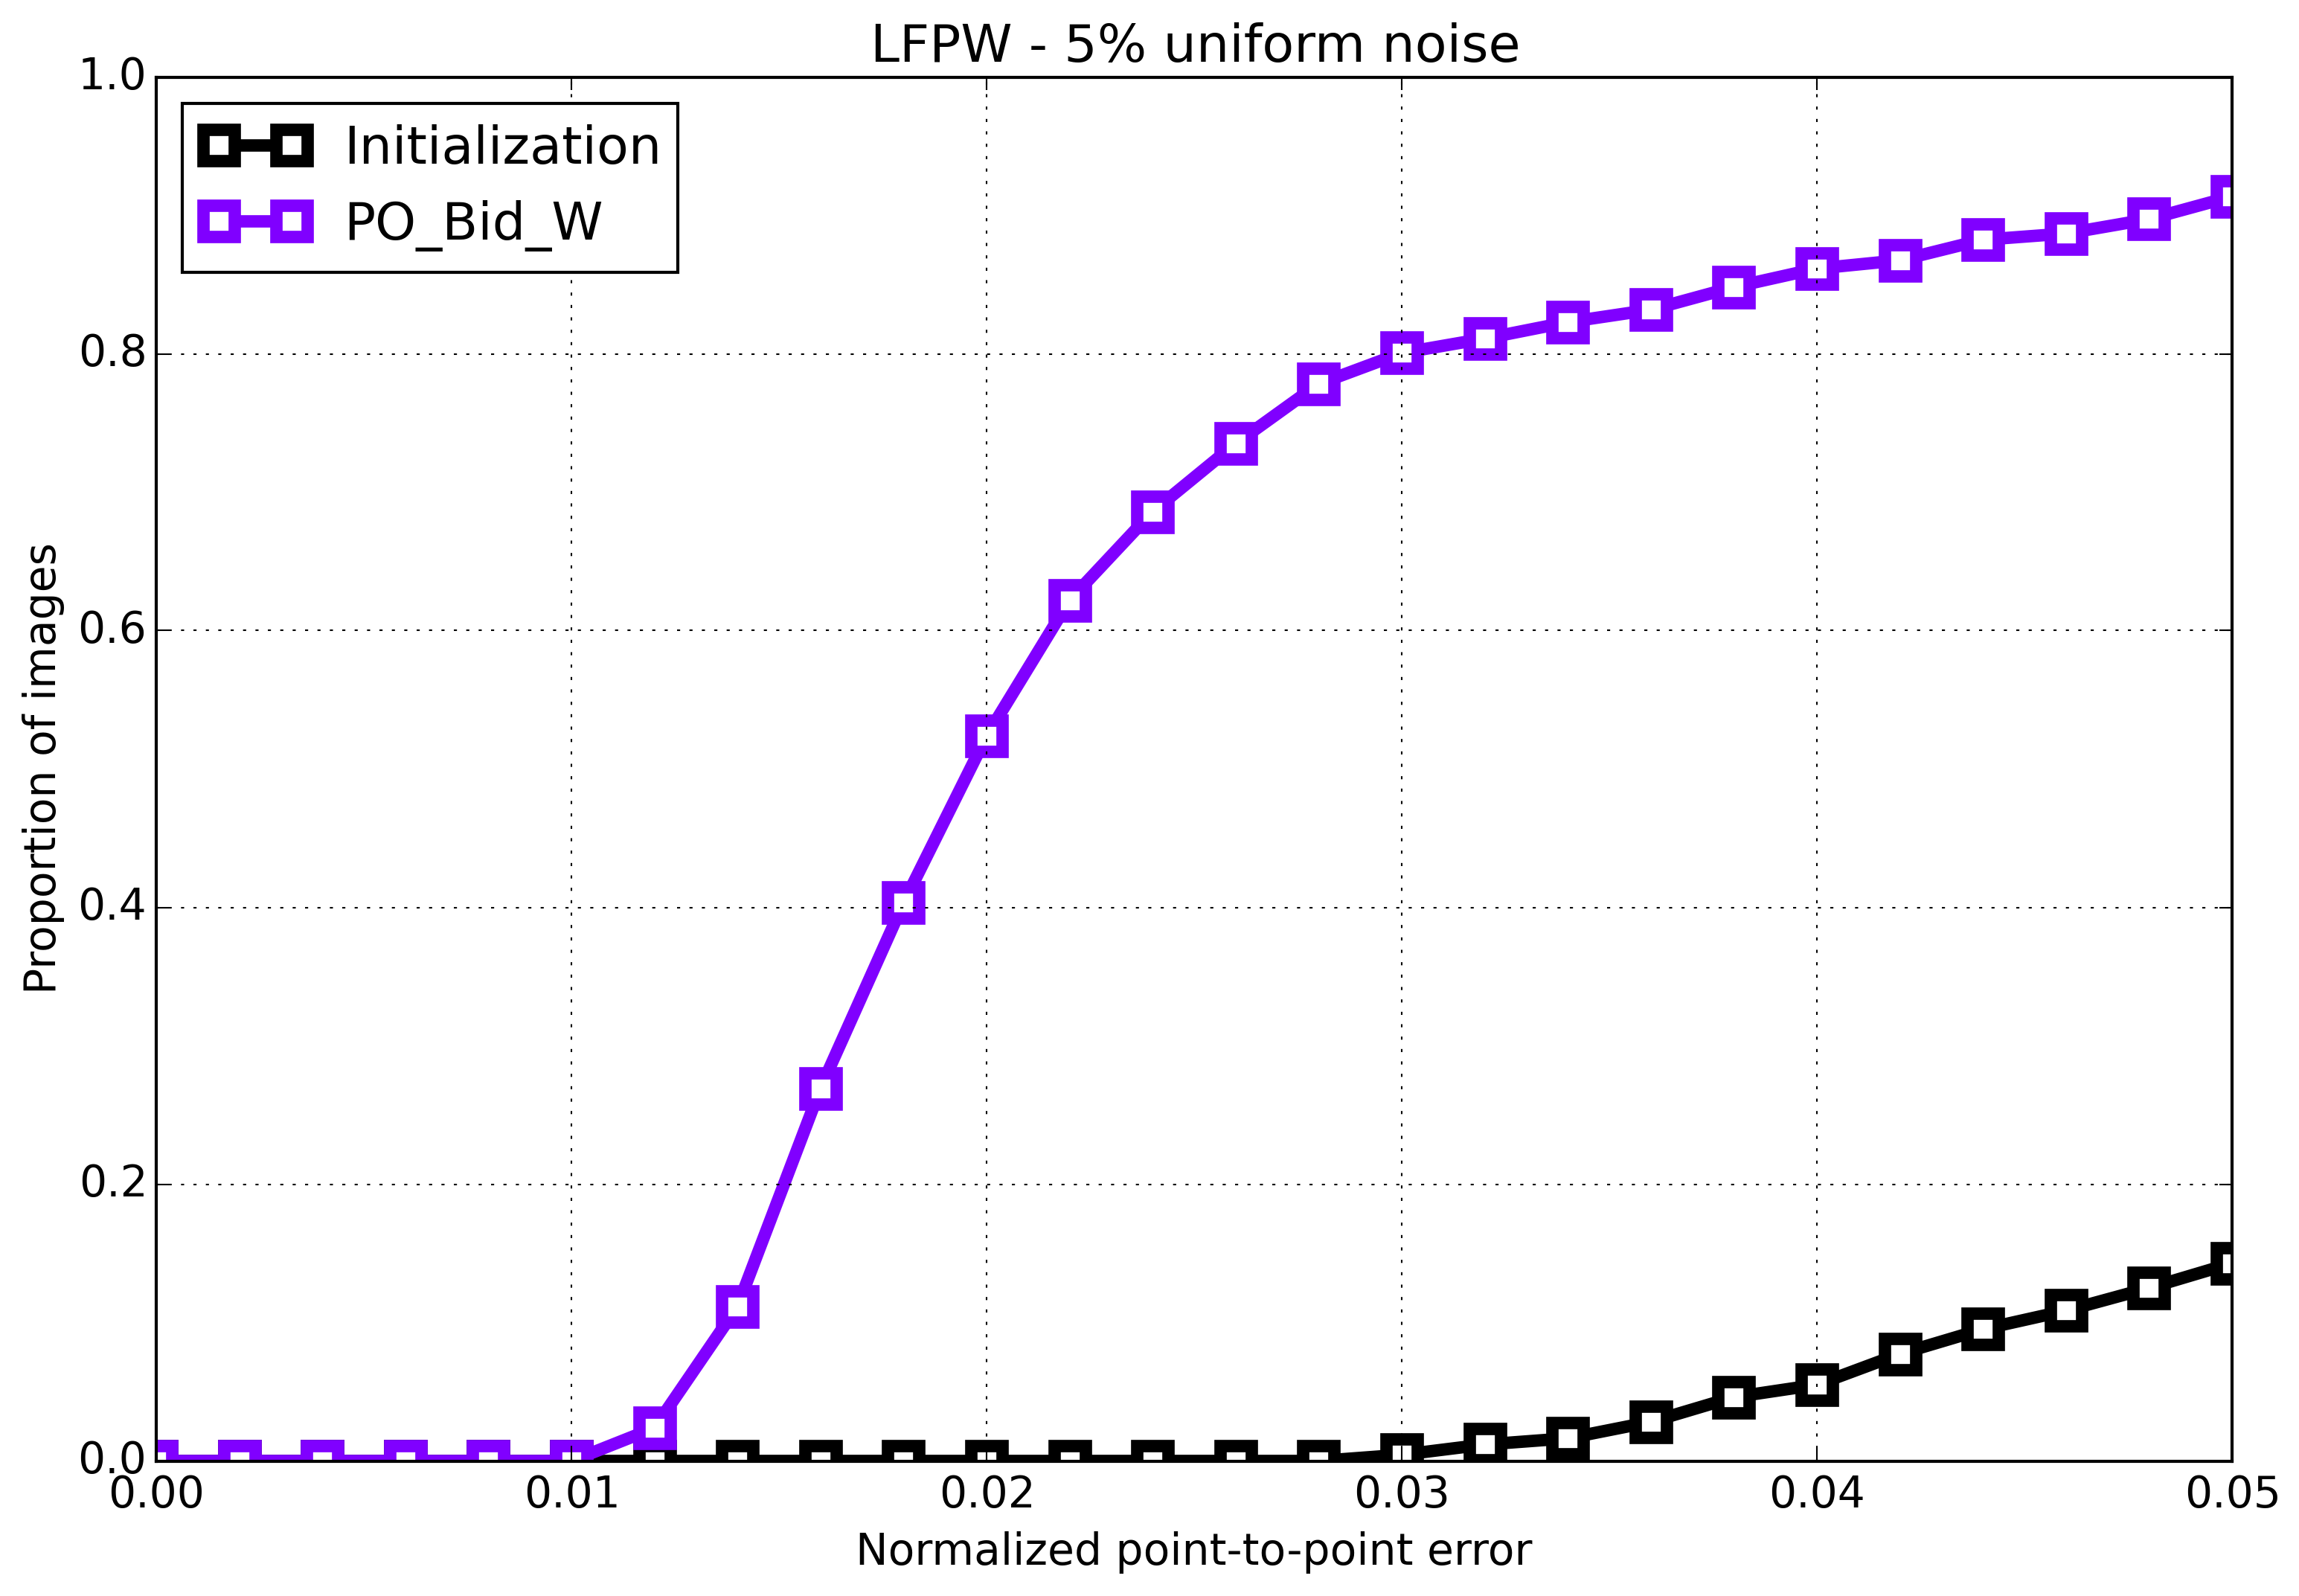
\includegraphics[width=\textwidth]{experiments/algorithms/po_w/ced_po_w_5.png}
	    \caption{Cumulative Error Distribution graph on the LFPW test dataset for all Project-Out Wiberg algorithms initialized with $5\%$ uniform noise.}
	    \label{fig:ced_po_w_5}
	\end{subfigure}
	\hfill
	\begin{subfigure}{0.48\textwidth}
	    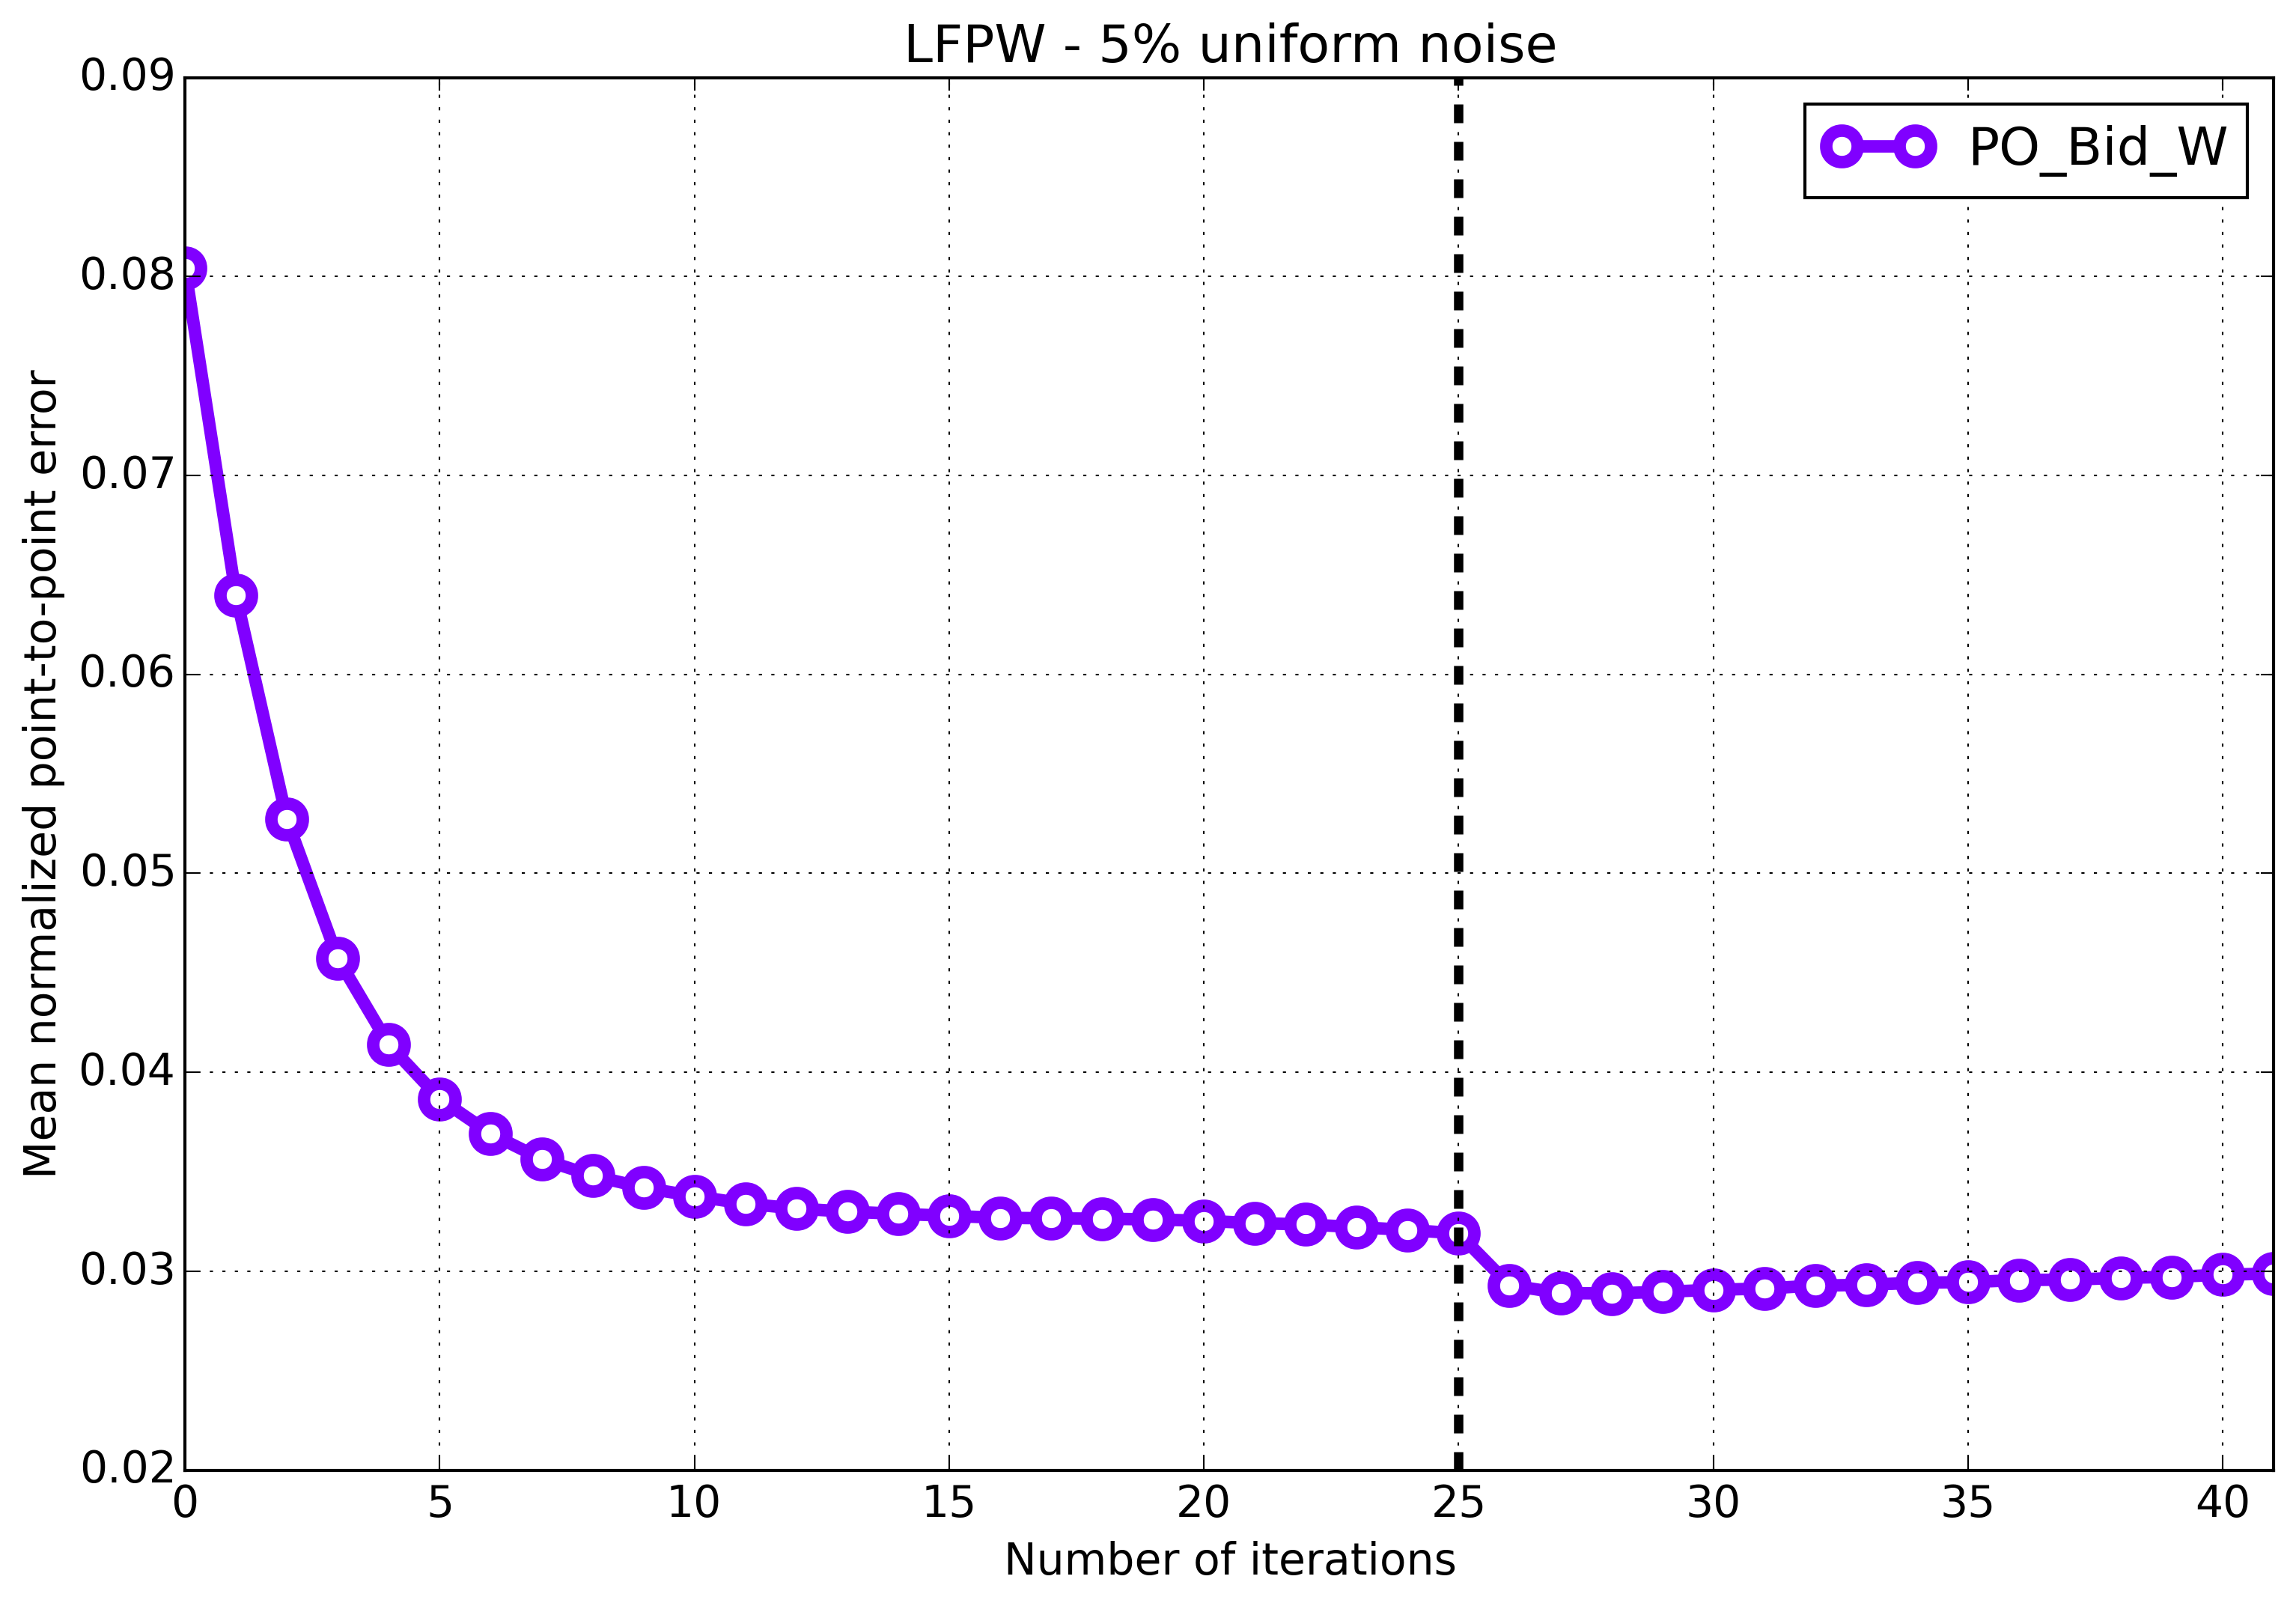
\includegraphics[width=\textwidth]{experiments/algorithms/po_w/mean_error_vs_iters_po_w_5.png}
	    \caption{Mean normalized point-to-point error vs number of iterations graph on the LFPW test dataset for all Project-Out Wiberg algorithms initialized with $5\%$ uniform noise.}
	    \label{fig:mean_error_vs_iters_po_w_5}
	\end{subfigure}
	\par\medskip
	\begin{subfigure}{0.48\textwidth}
	    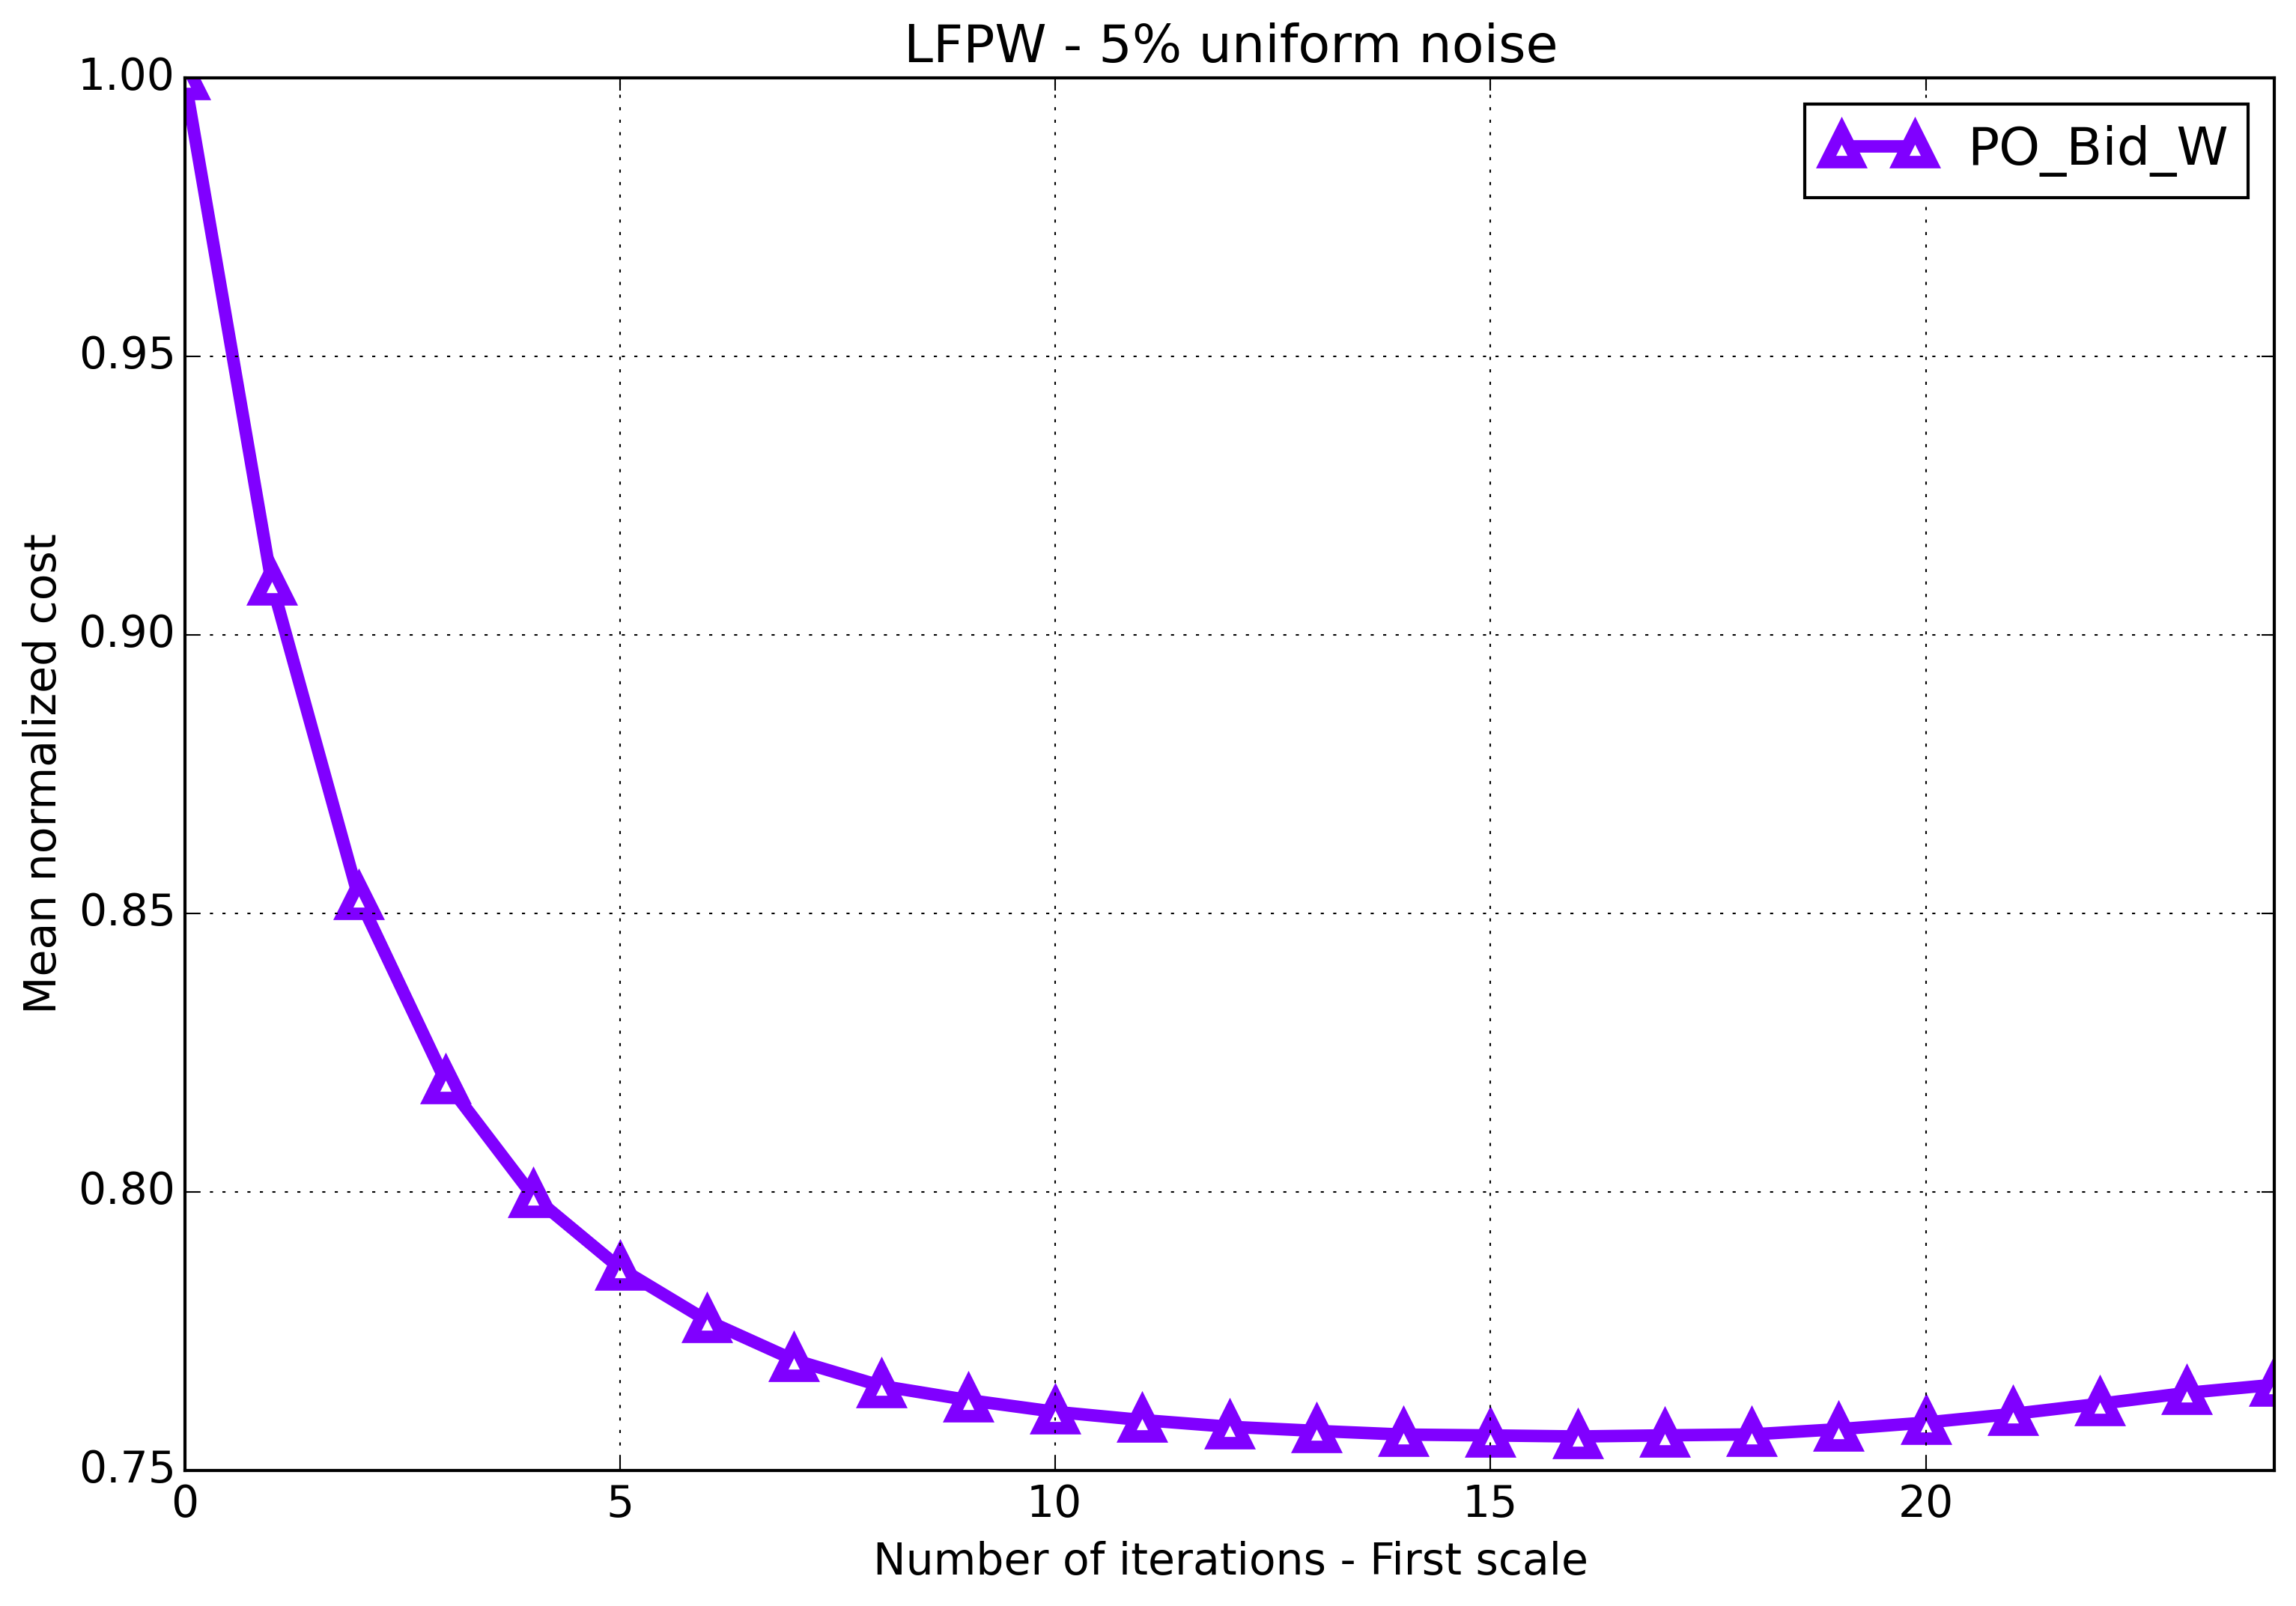
\includegraphics[width=\textwidth]{experiments/algorithms/po_w/mean_cost_vs_iters1_po_w_5.png}
	    \caption{Mean normalized cost vs number of first scale iterations graph on the LFPW test dataset for all Project-Out Wiberg algorithms initialized with $5\%$ uniform noise.}
	    \label{fig:mean_cost_vs_iters1_po_w_5}
	\end{subfigure}
	\hfill
	\begin{subfigure}{0.48\textwidth}
	    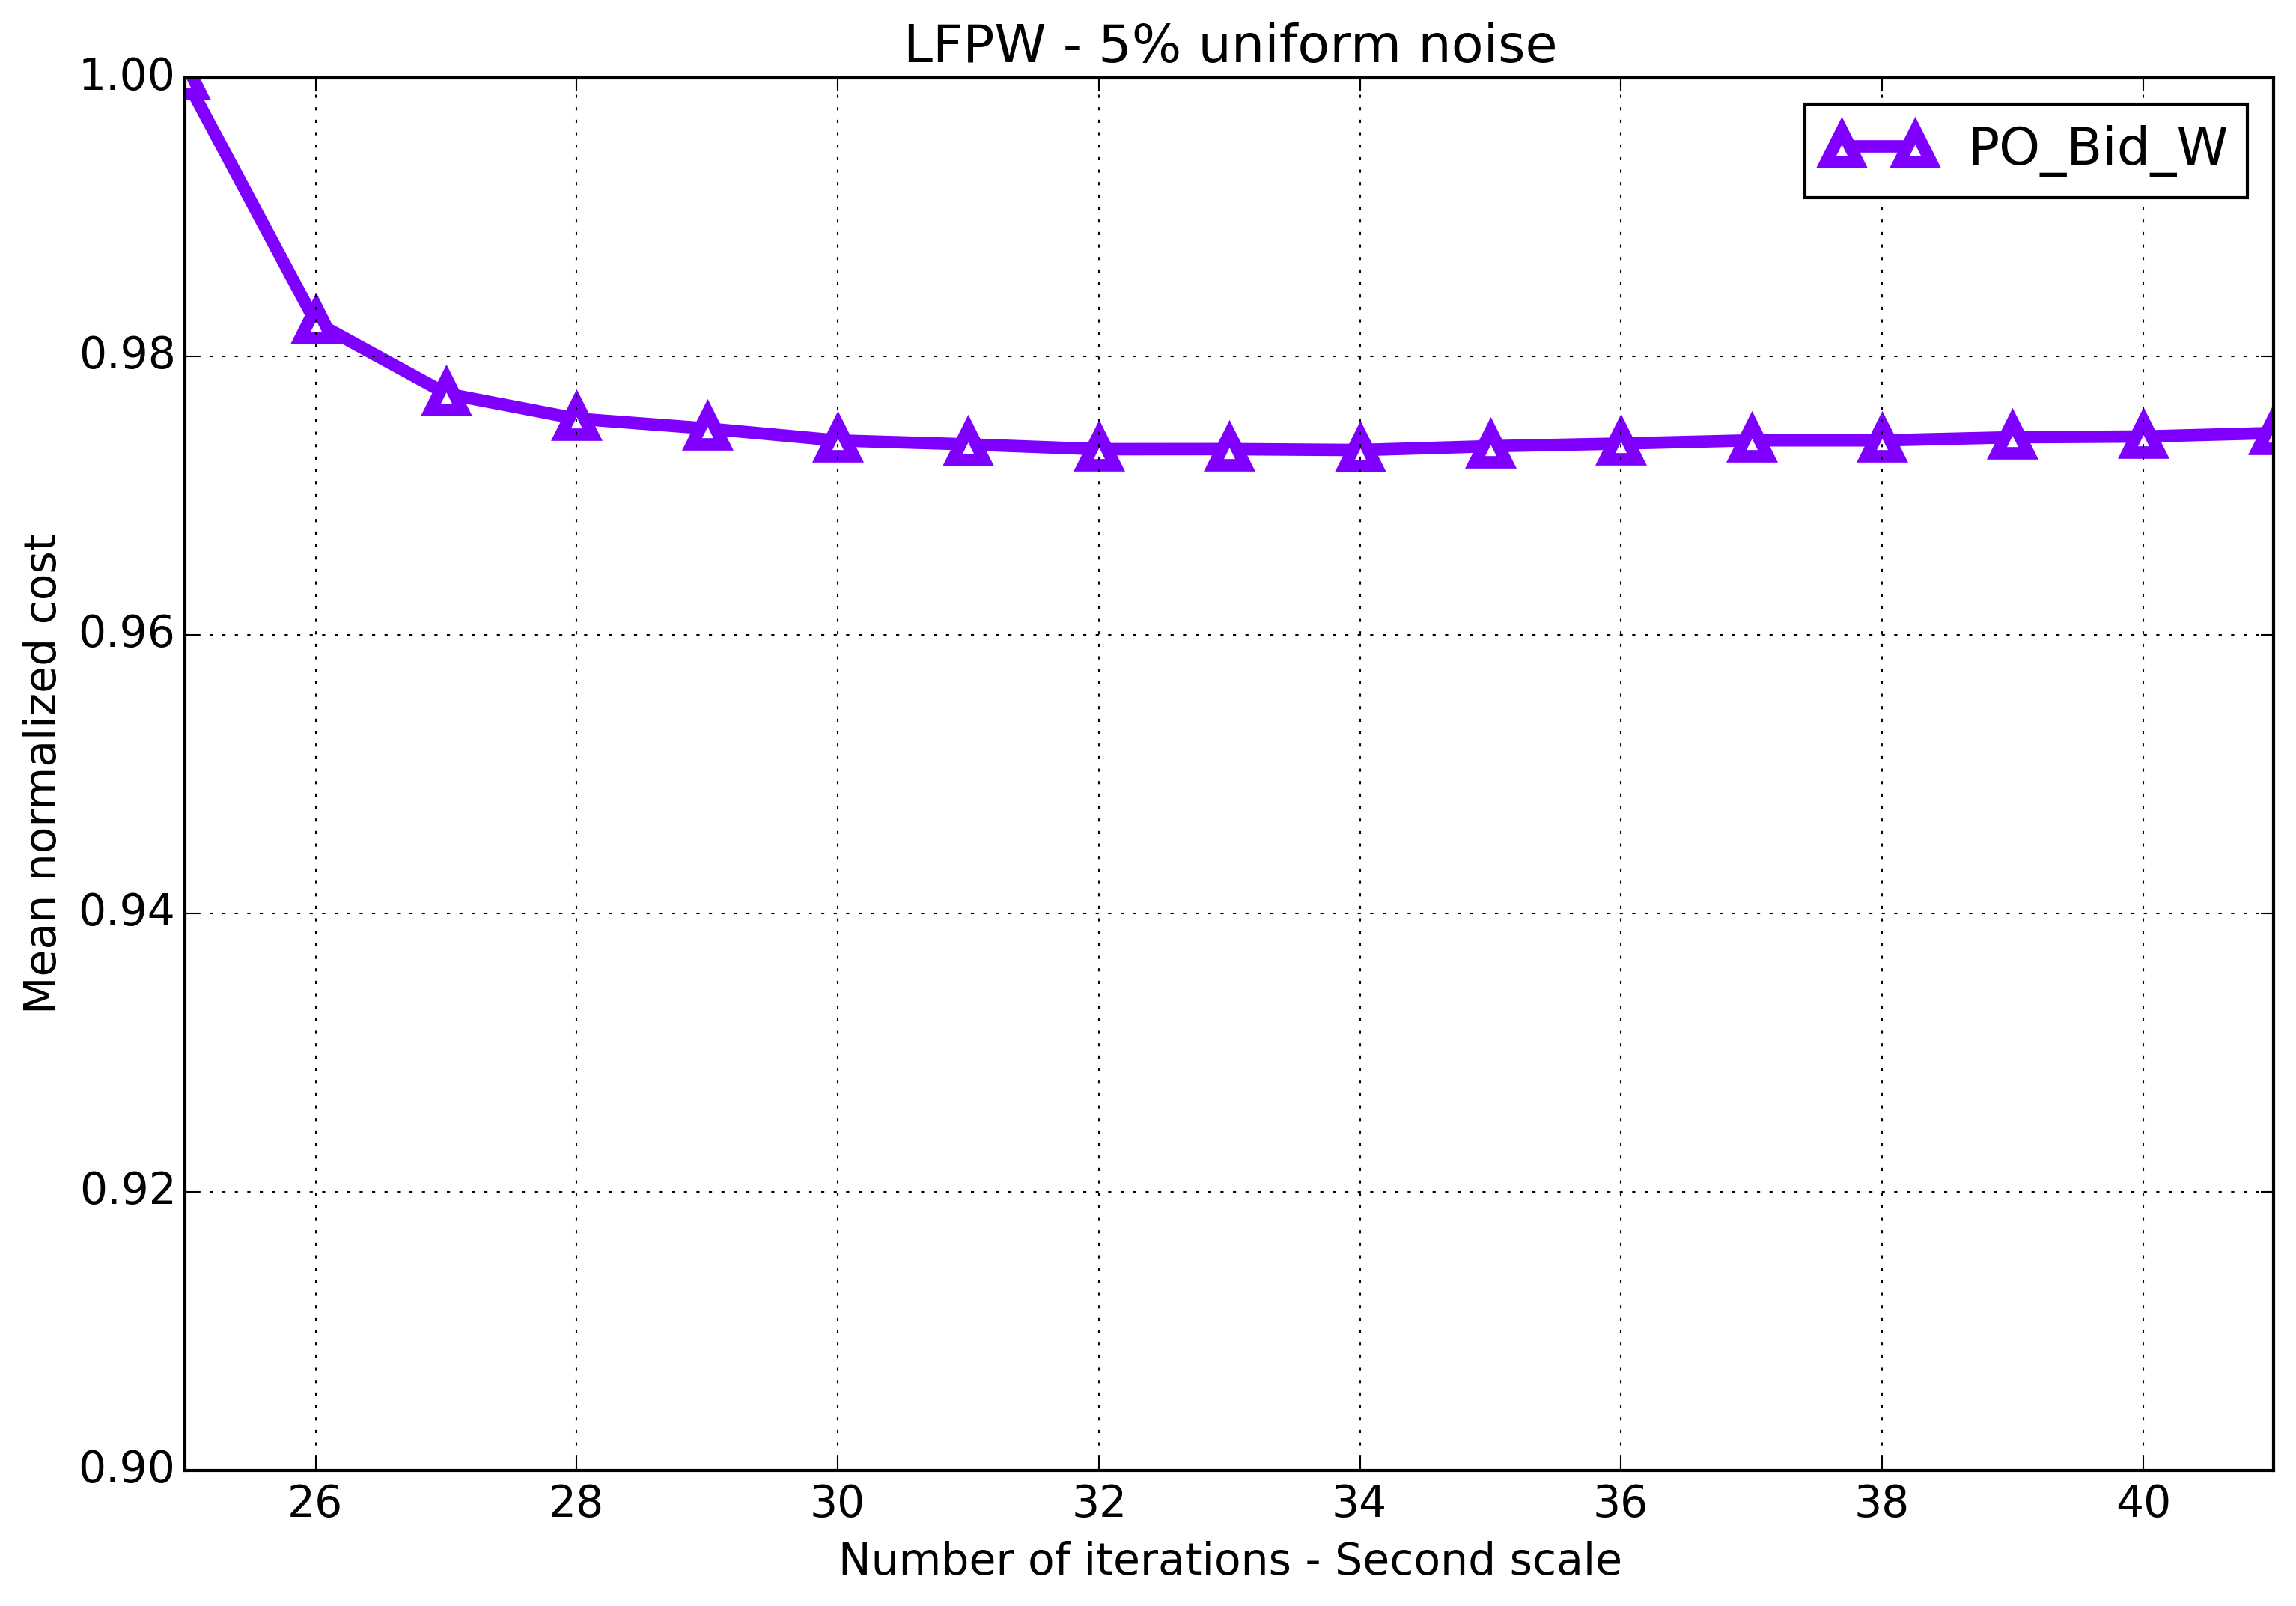
\includegraphics[width=\textwidth]{experiments/algorithms/po_w/mean_cost_vs_iters2_po_w_5.png}
	    \caption{Mean normalized cost vs number of second scale iterations graph on the LFPW test dataset for all Project-Out Wiberg algorithms initialized with $5\%$ uniform noise.}
	    \label{fig:mean_cost_vs_iters2_po_w_5}
	\end{subfigure}
	\label{fig:po_w_5}
	\caption{}
\end{figure*}


% \begin{figure}[h!]
%     \centering
%     \includegraphics[width=0.50\textwidth]{experiments/algorithms/ssd_gn/ced_ssd_gn_4.png}
%     \caption{CED graph on the LFPW test dataset for all SSD Gauss-Newton algorithms initialized with $4$\% of uniform noise.}
%     \label{fig:ced_po_asymmetric_gn_4}
% \end{figure}




% \begin{figure}[h!]
%     \centering
%     \includegraphics[width=0.50\textwidth]{experiments/algorithms/ssd_gn/mean_error_vs_iters_ssd_gn_4.png}
%     \caption{Mean normalized point-to-point error vs number of iterations graph on the LFPW test dataset for all SSD Gauss-Newton algorithms initialized with $4$\% of uniform noise}
%     \label{fig:mean_error_vs_iters_po_asymmetric_gn_4}
% \end{figure}


\subsubsection{Weighted Bayesian project-out}

\begin{figure}[h!]
	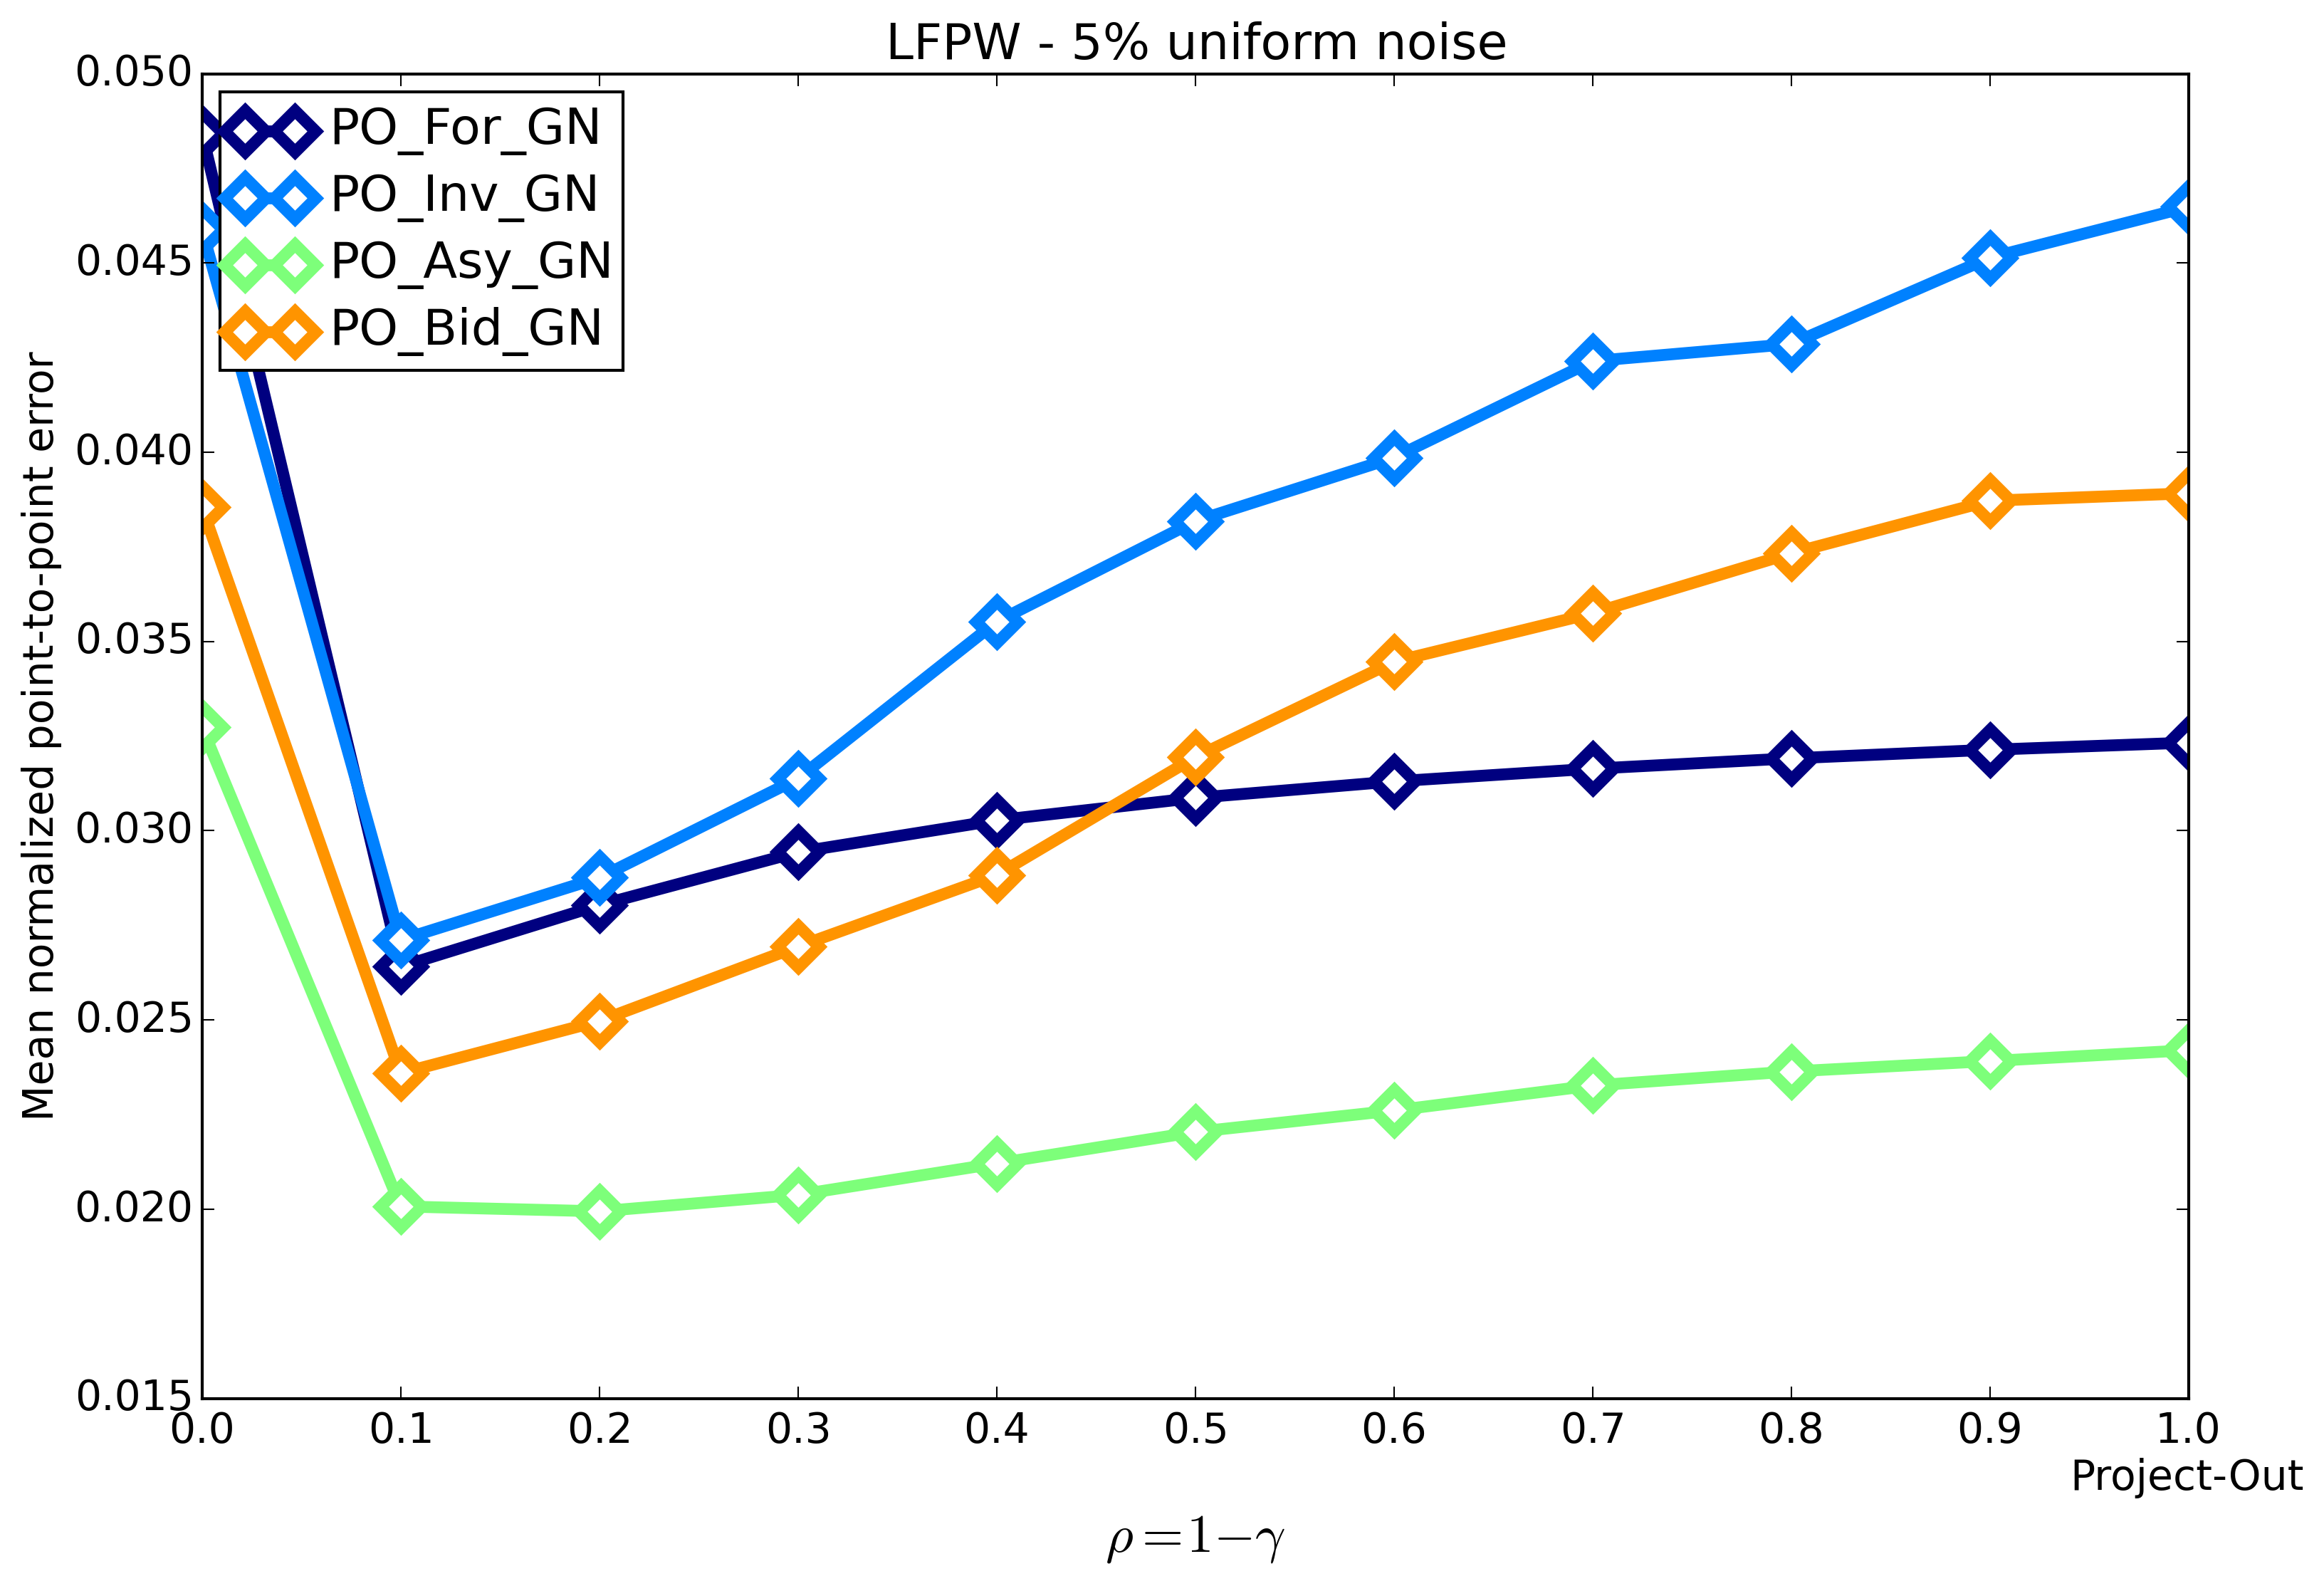
\includegraphics[width=0.48\textwidth]{experiments/rho/mean_error_vs_rho_5.png}
    \caption{Mean normalized point-to-point error vs rho on the LFPW test dataset for all PO Gauss-Newton algorithms initialized with $5\%$ uniform noise.}
    \label{fig:ced_ssd_gn_5}
\end{figure}

\subsubsection{Optimal asymmetric composition}

\begin{figure}[h!]
    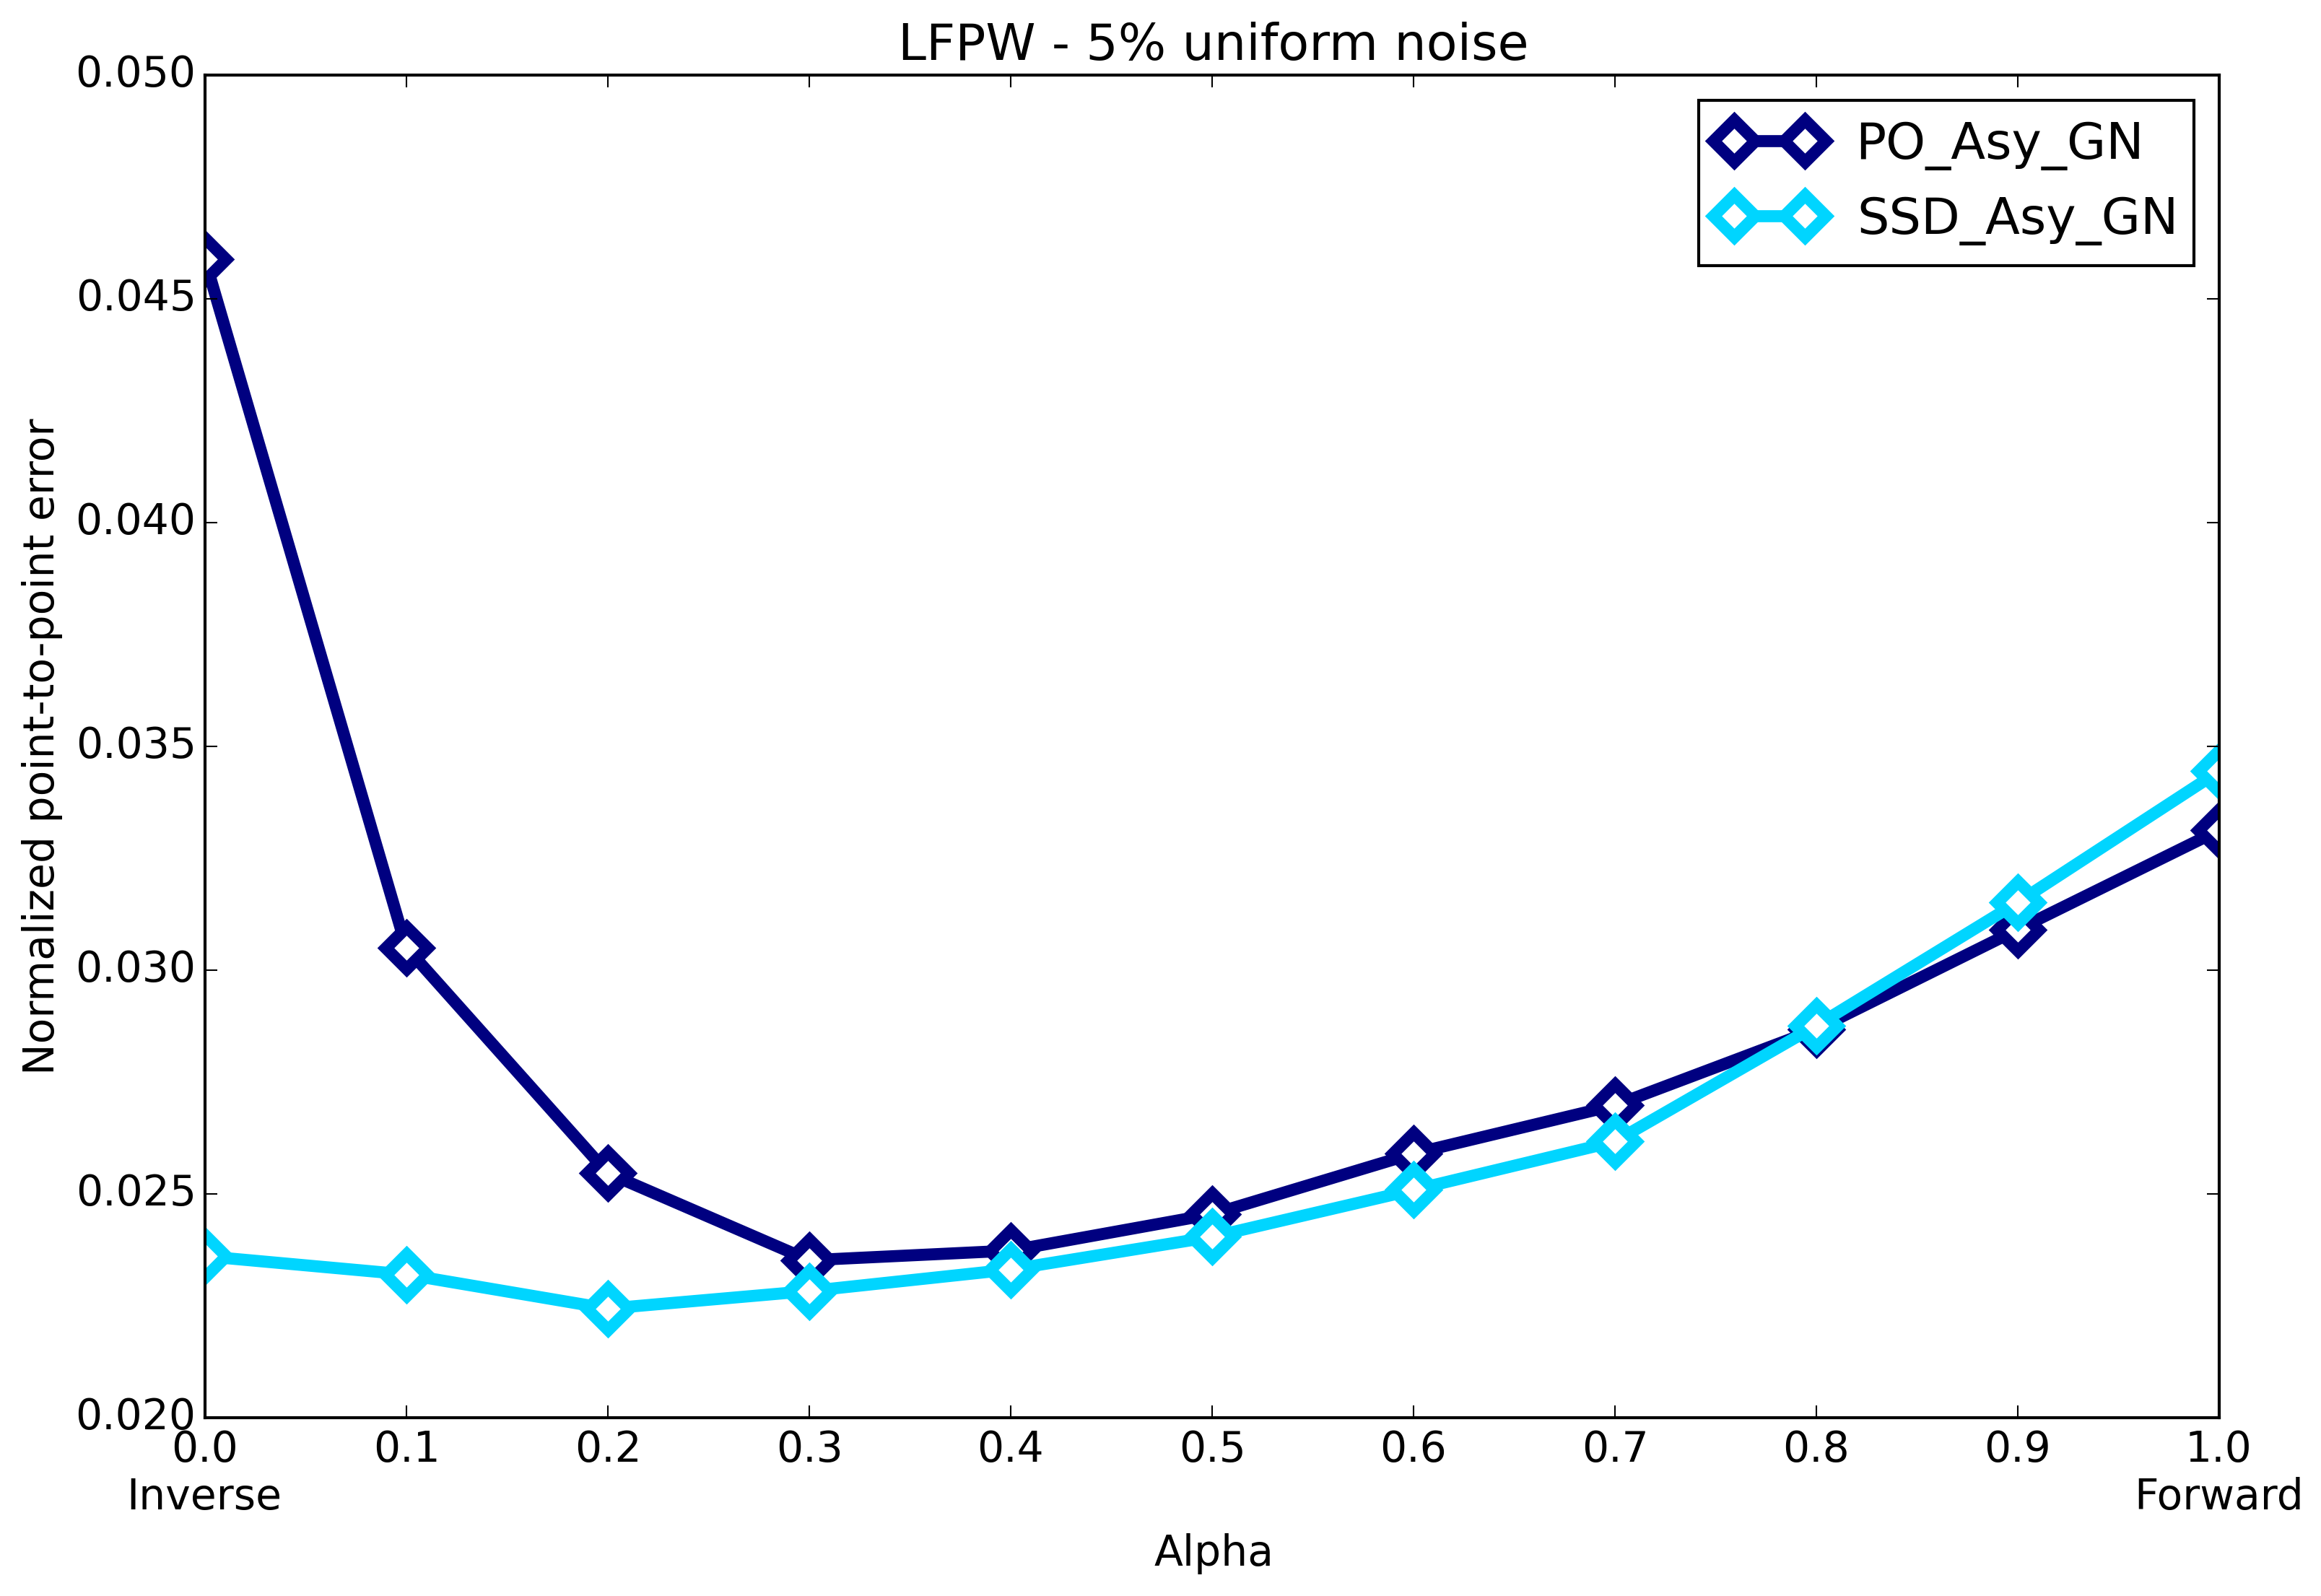
\includegraphics[width=0.48\textwidth]{experiments/alpha/mean_error_vs_alpha_5.png}
    \caption{Mean normalized point-to-point error vs alpha on the LFPW test dataset for all Asymmetric Gauss-Newton algorithms initialized with $5\%$ uniform noise.}
    \label{fig:ced_ssd_gn_5}
\end{figure}

\subsubsection{Sampling}

\begin{figure}[h!]
    \centering
    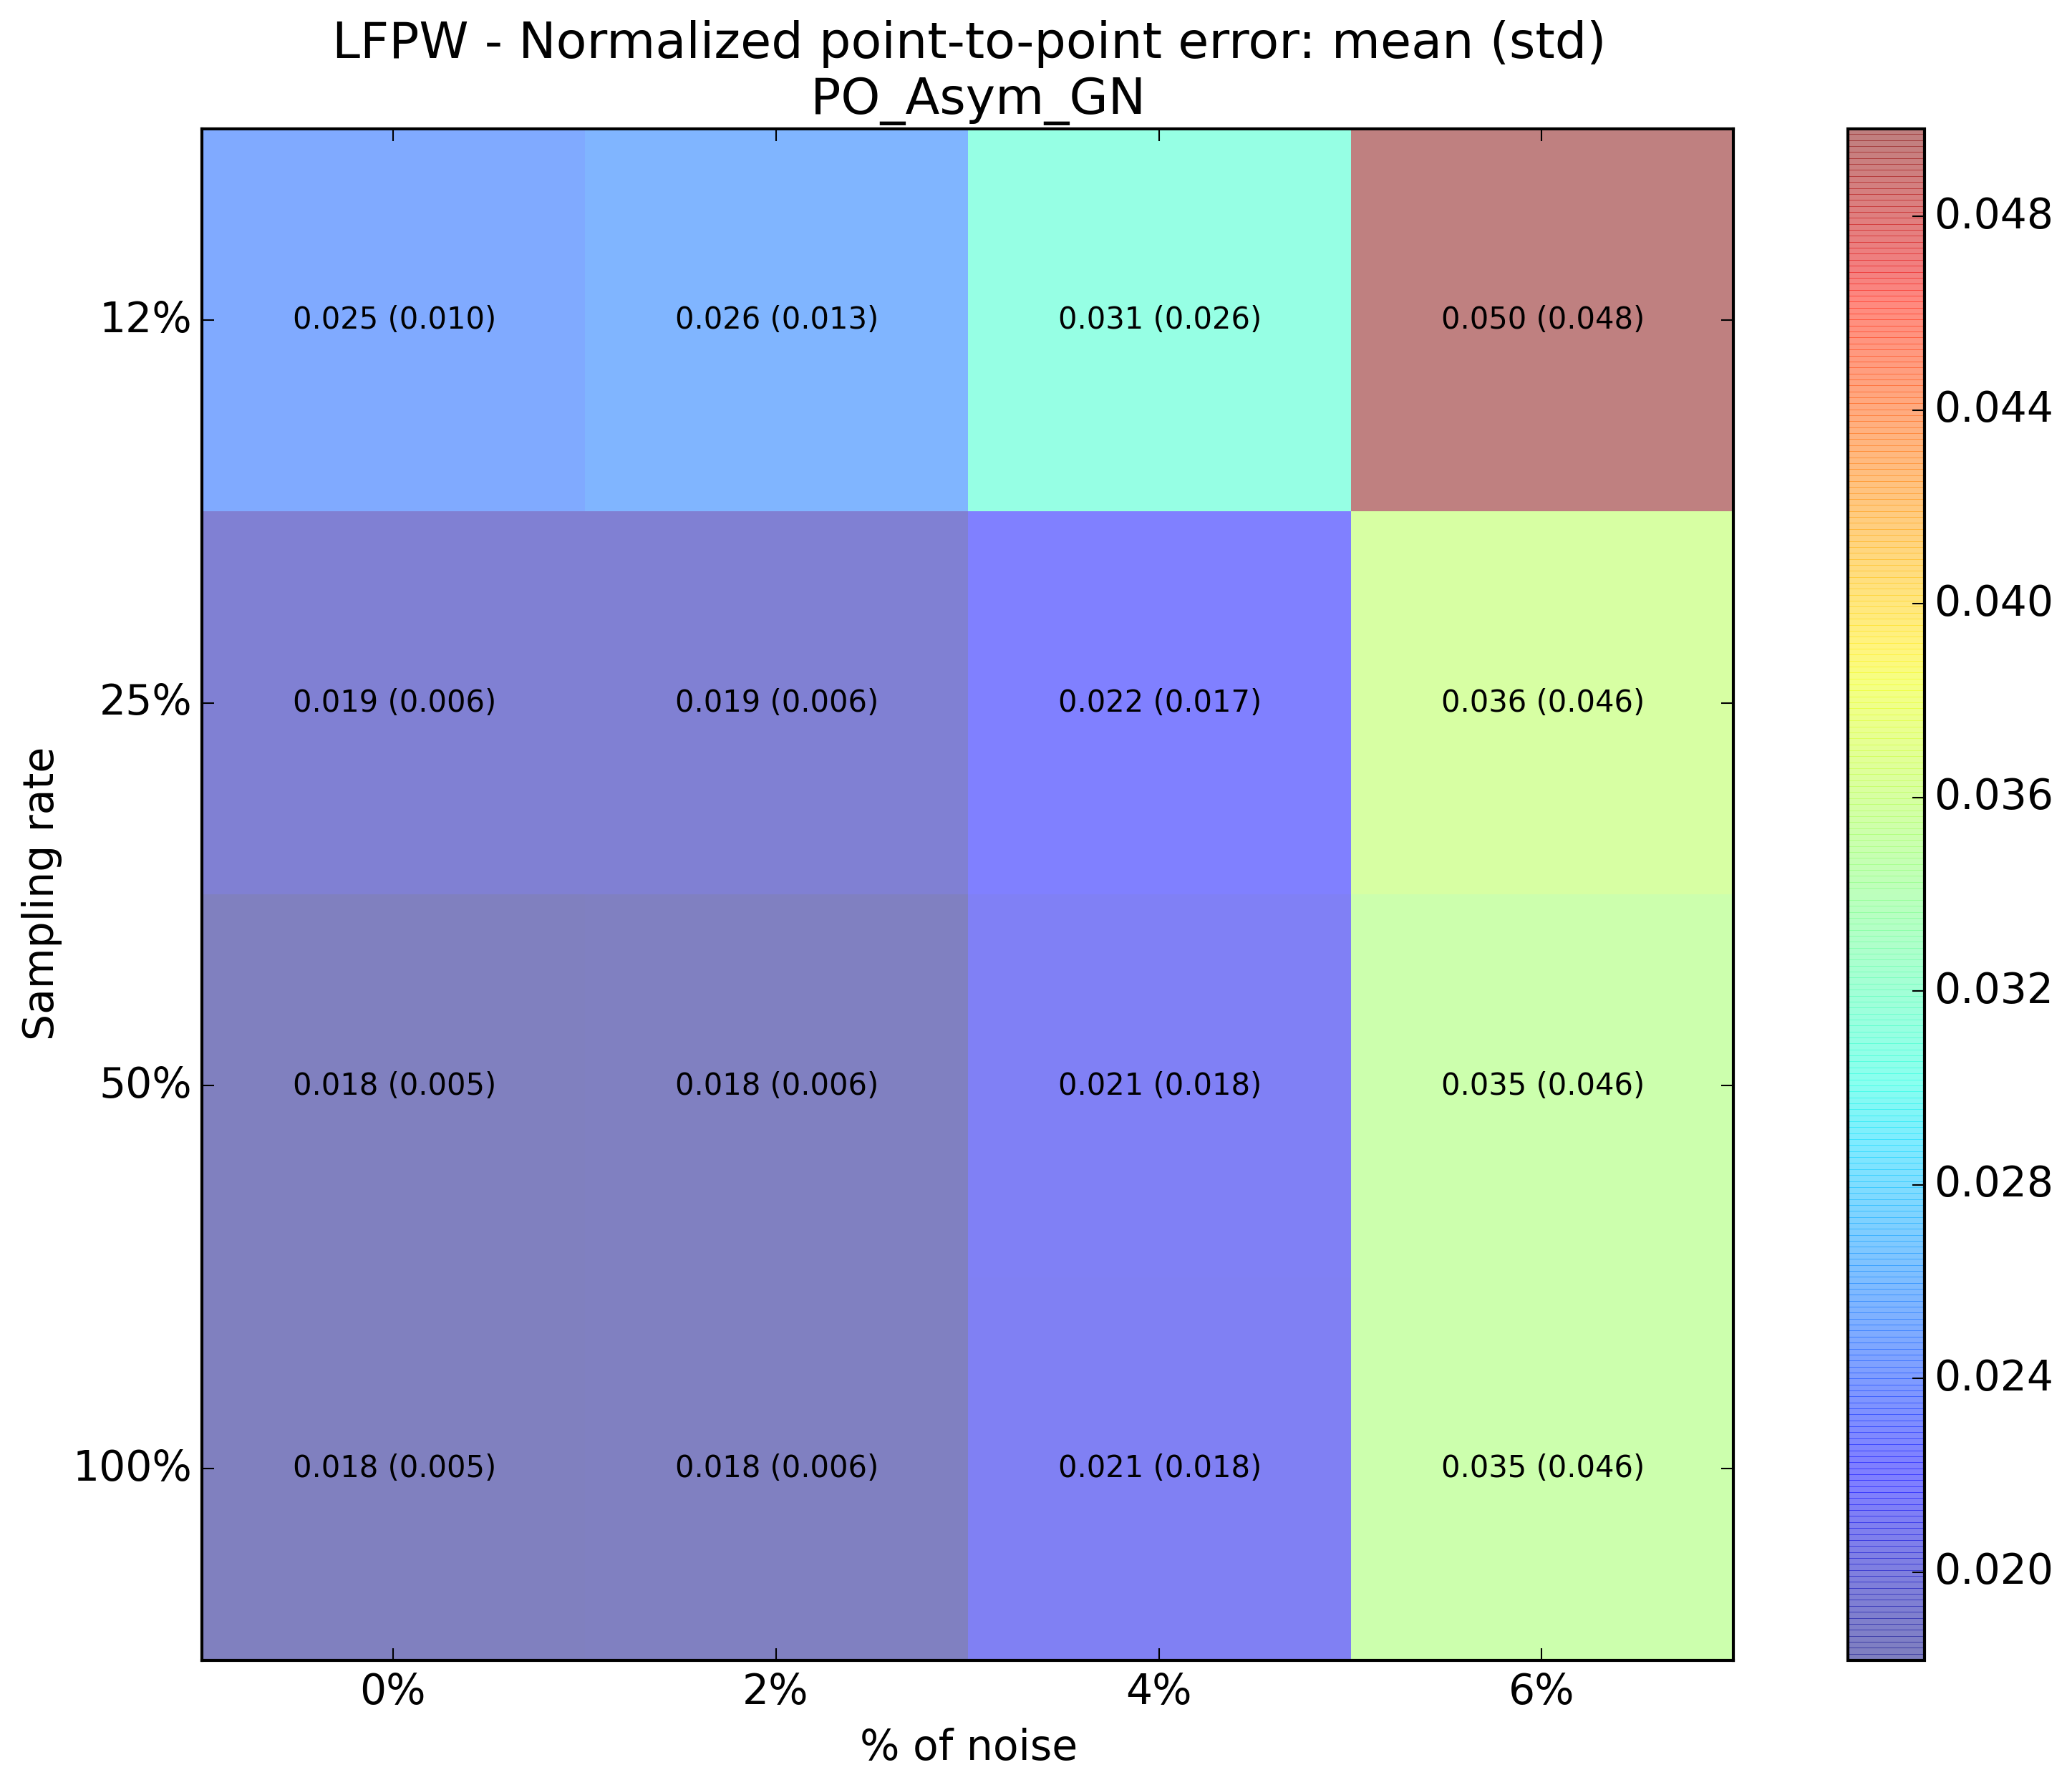
\includegraphics[width=0.45\textwidth]{experiments/sampling/po_asymmetric_gn/noise_vs_sampling_po_asymmetric.png}
    \caption{Mean and Std of normalized point-to-point error obtained on the LFPW test dataset by the Project-Out Asymmetric Gauss-Newton algorithm for different sampling rates versus different amounts of noise \% on the initialization.}
    \label{fig:noise_vs_sampling_po_asymmetric}
\end{figure}

\begin{figure}[h!]
    \centering
    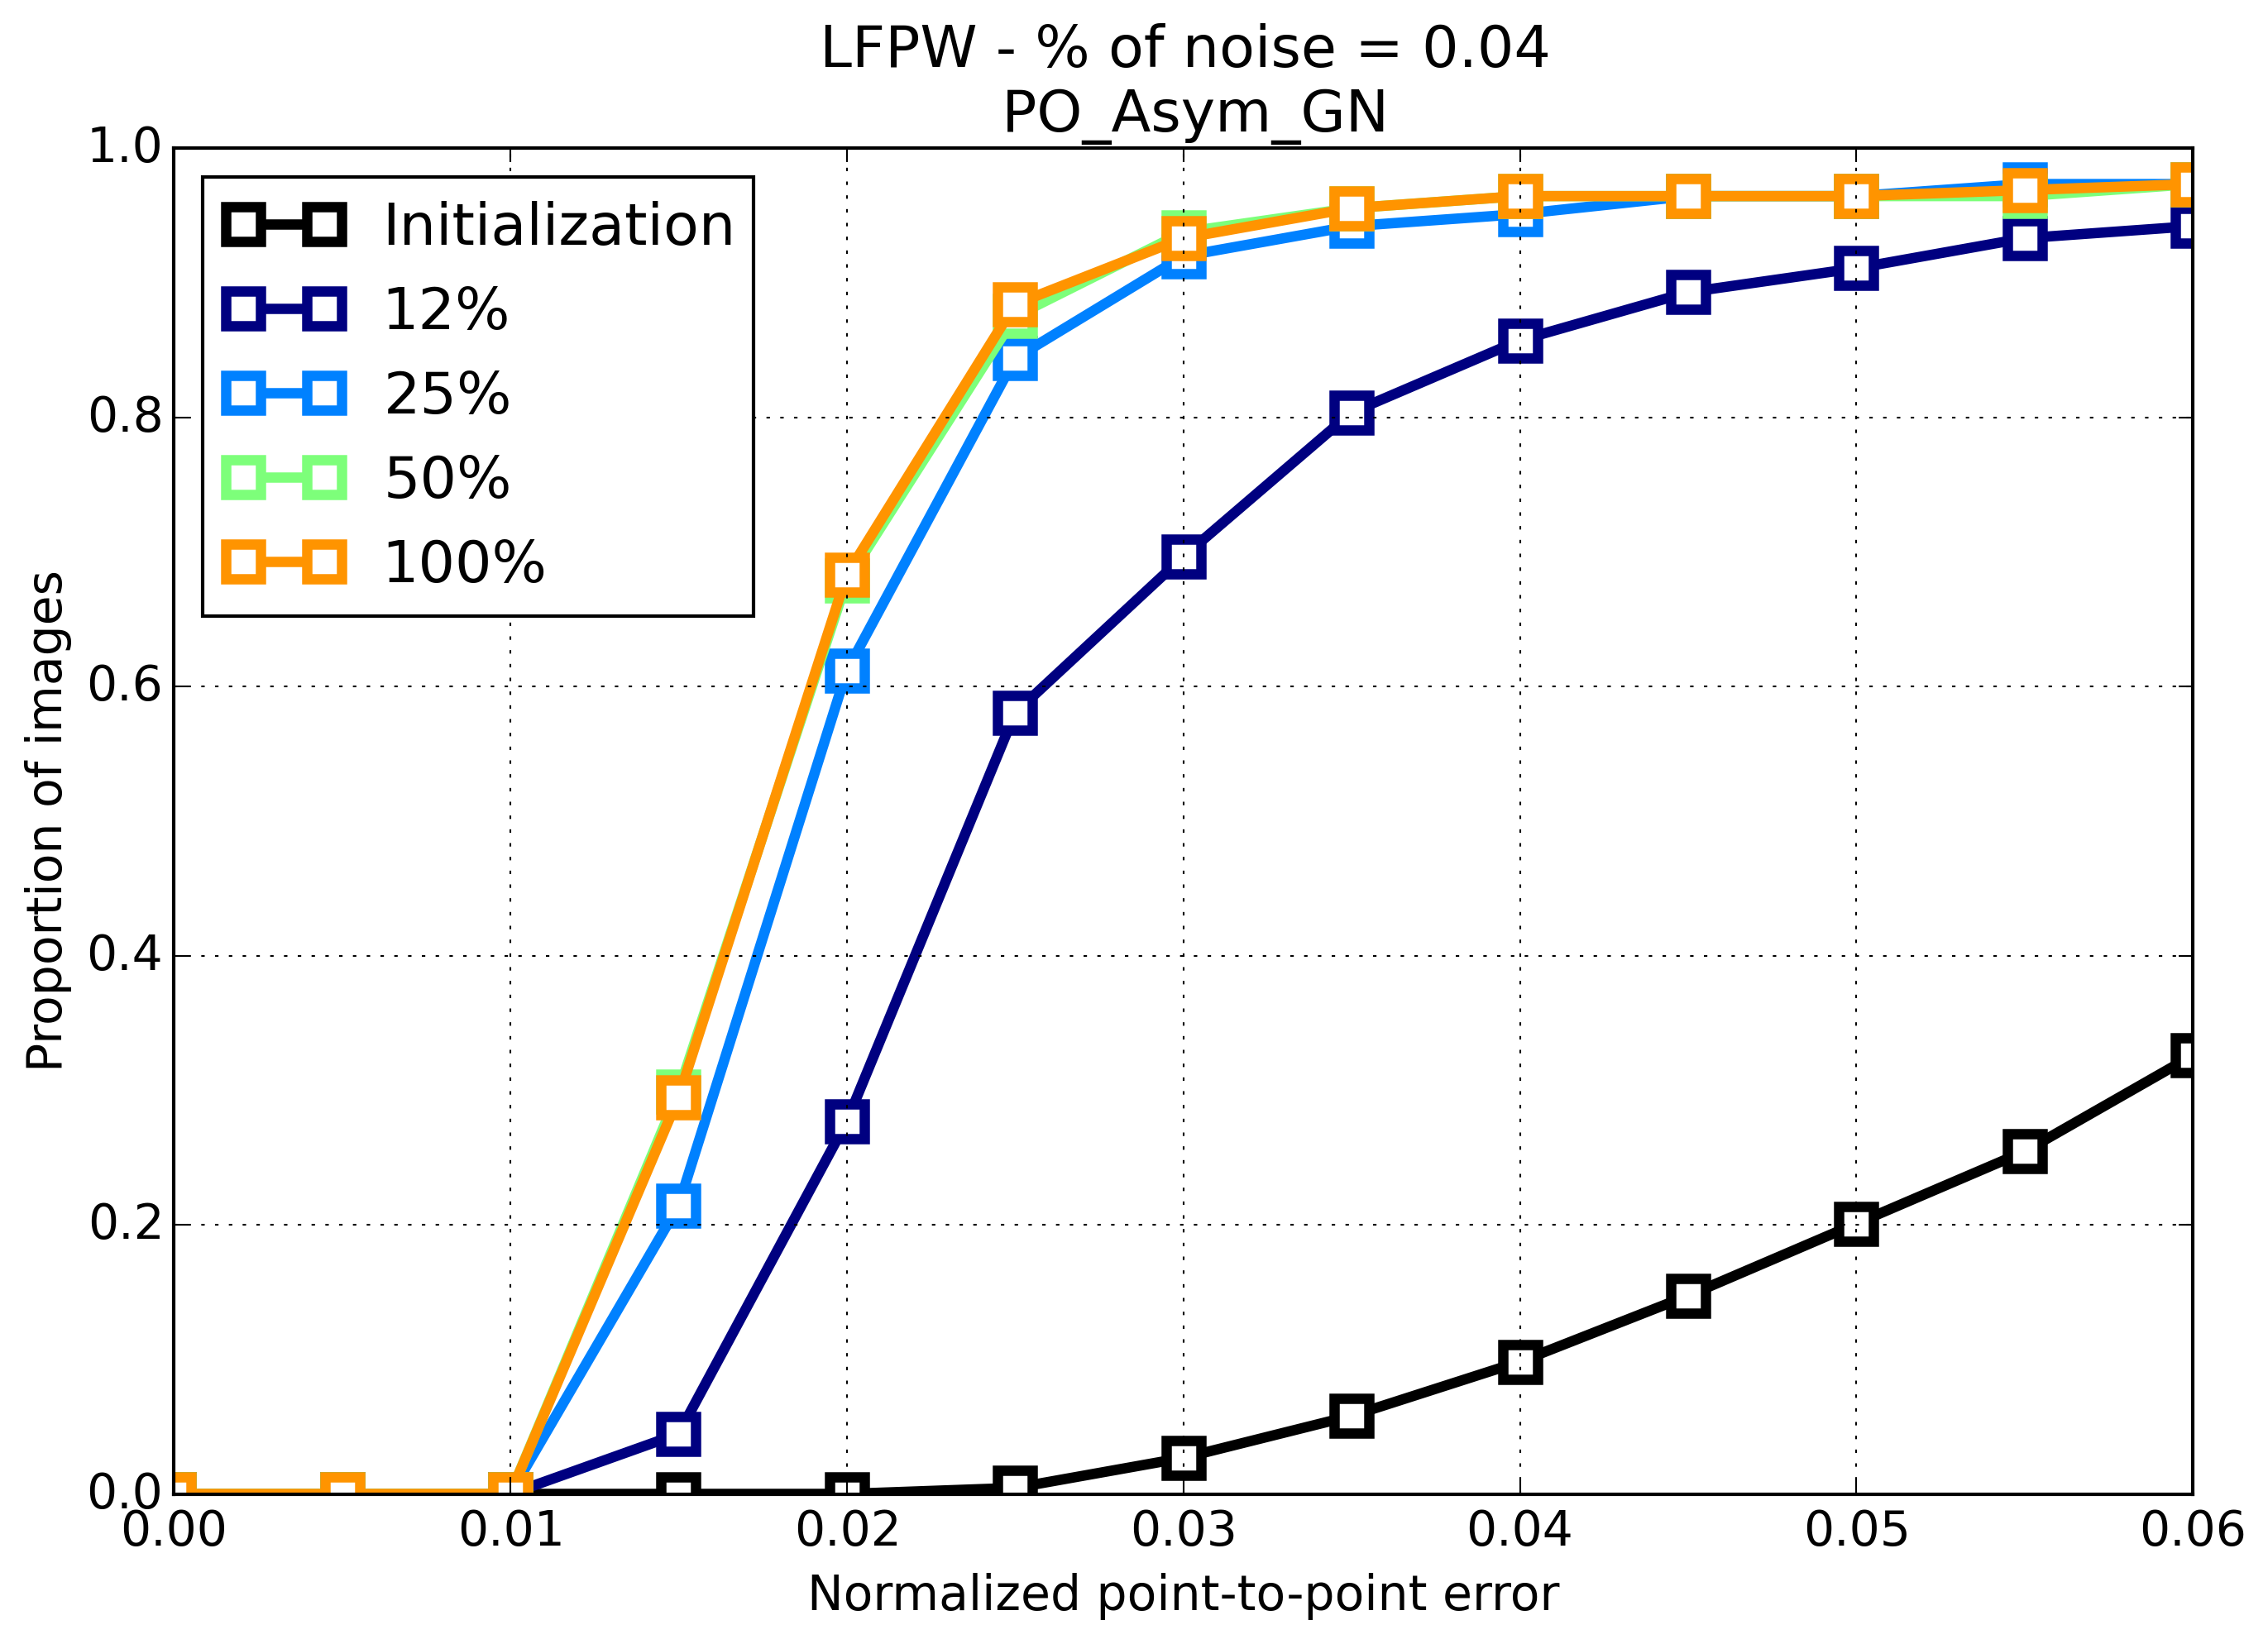
\includegraphics[width=0.50\textwidth]{experiments/sampling/po_asymmetric_gn/ced_po_asymmetric_gn_4.png}
    \caption{CED graph on the LFPW test dataset obtained by the Project-Out Asymmetric Gauss-Newton algorithm for $4$\% noise on the initialization.}
    \label{fig:ced_po_asymmetric_gn_4}
\end{figure}

\begin{figure}[h!]
    \centering
    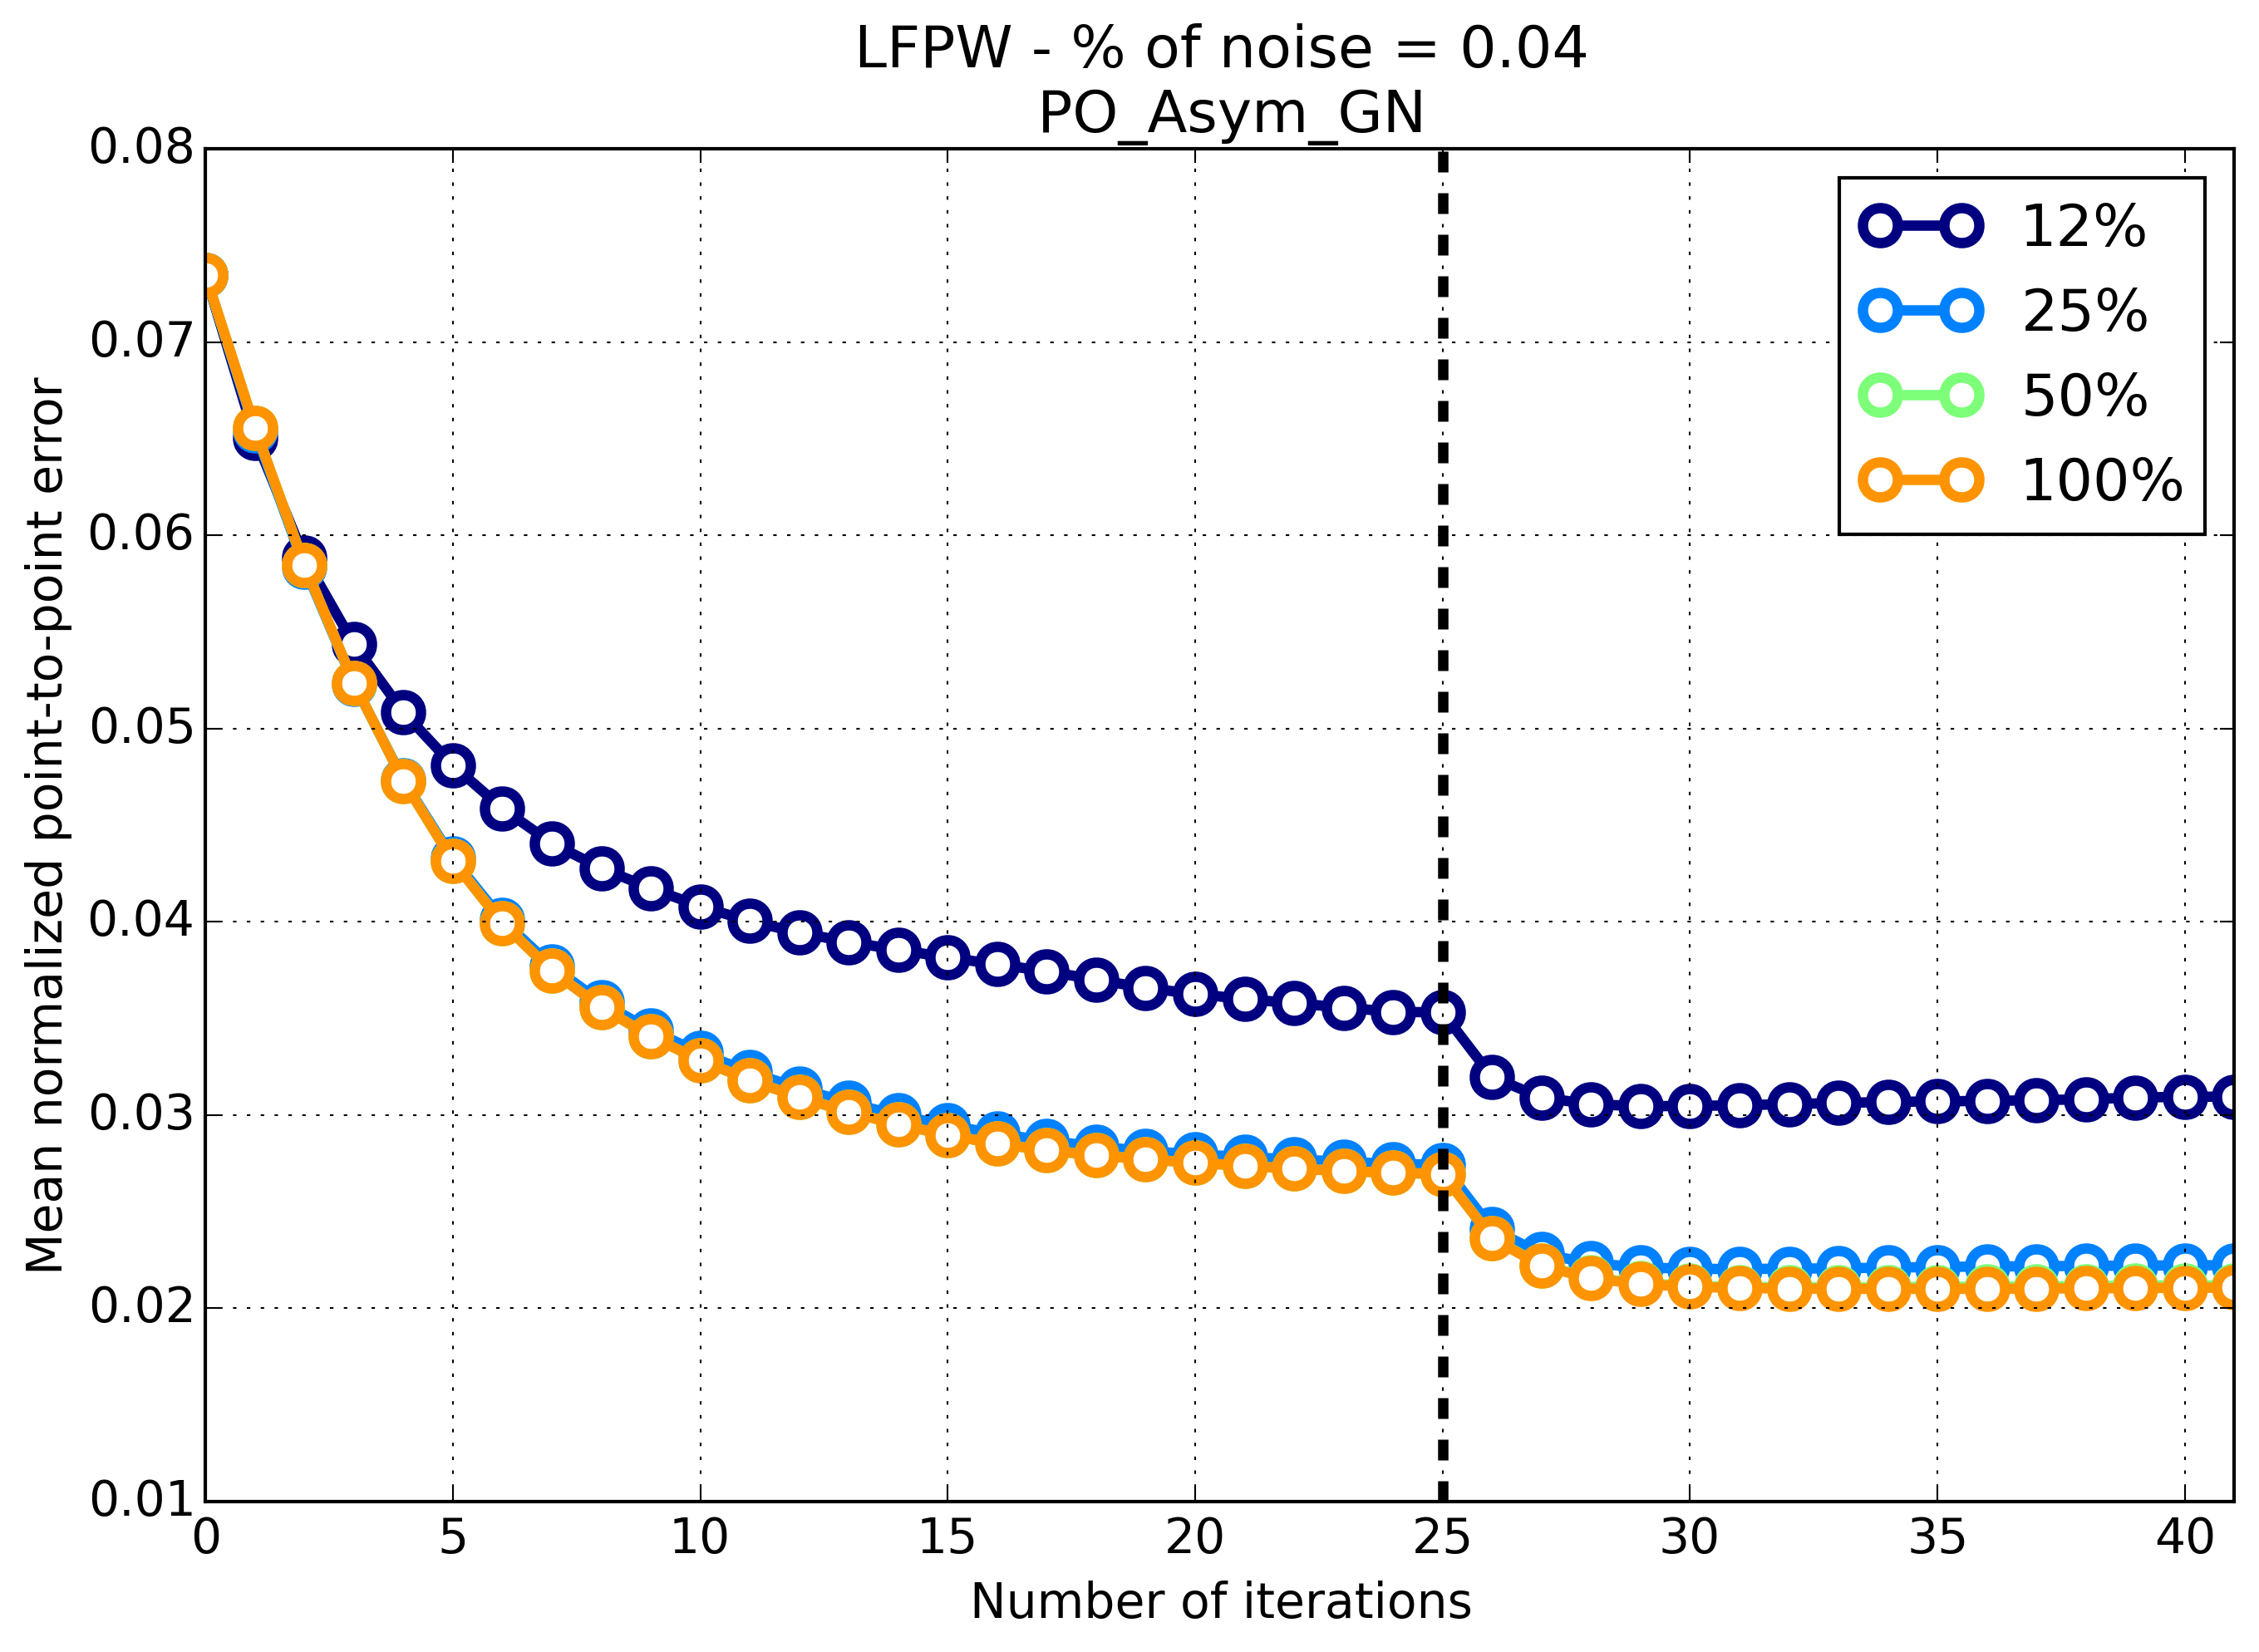
\includegraphics[width=0.50\textwidth]{experiments/sampling/po_asymmetric_gn/mean_error_vs_iters_po_asymmetric_gn_4.png}
    \caption{Mean normalized point-to-point error vs number of iterations graph on the LFPW test dataset obtained by the Project-Out Asymmetric Gauss-Newton algorithm for $4$\% noise on the initialization.}
    \label{fig:mean_error_vs_iters_po_asymmetric_gn_4}
\end{figure}

\begin{figure}[h!]
    \centering
    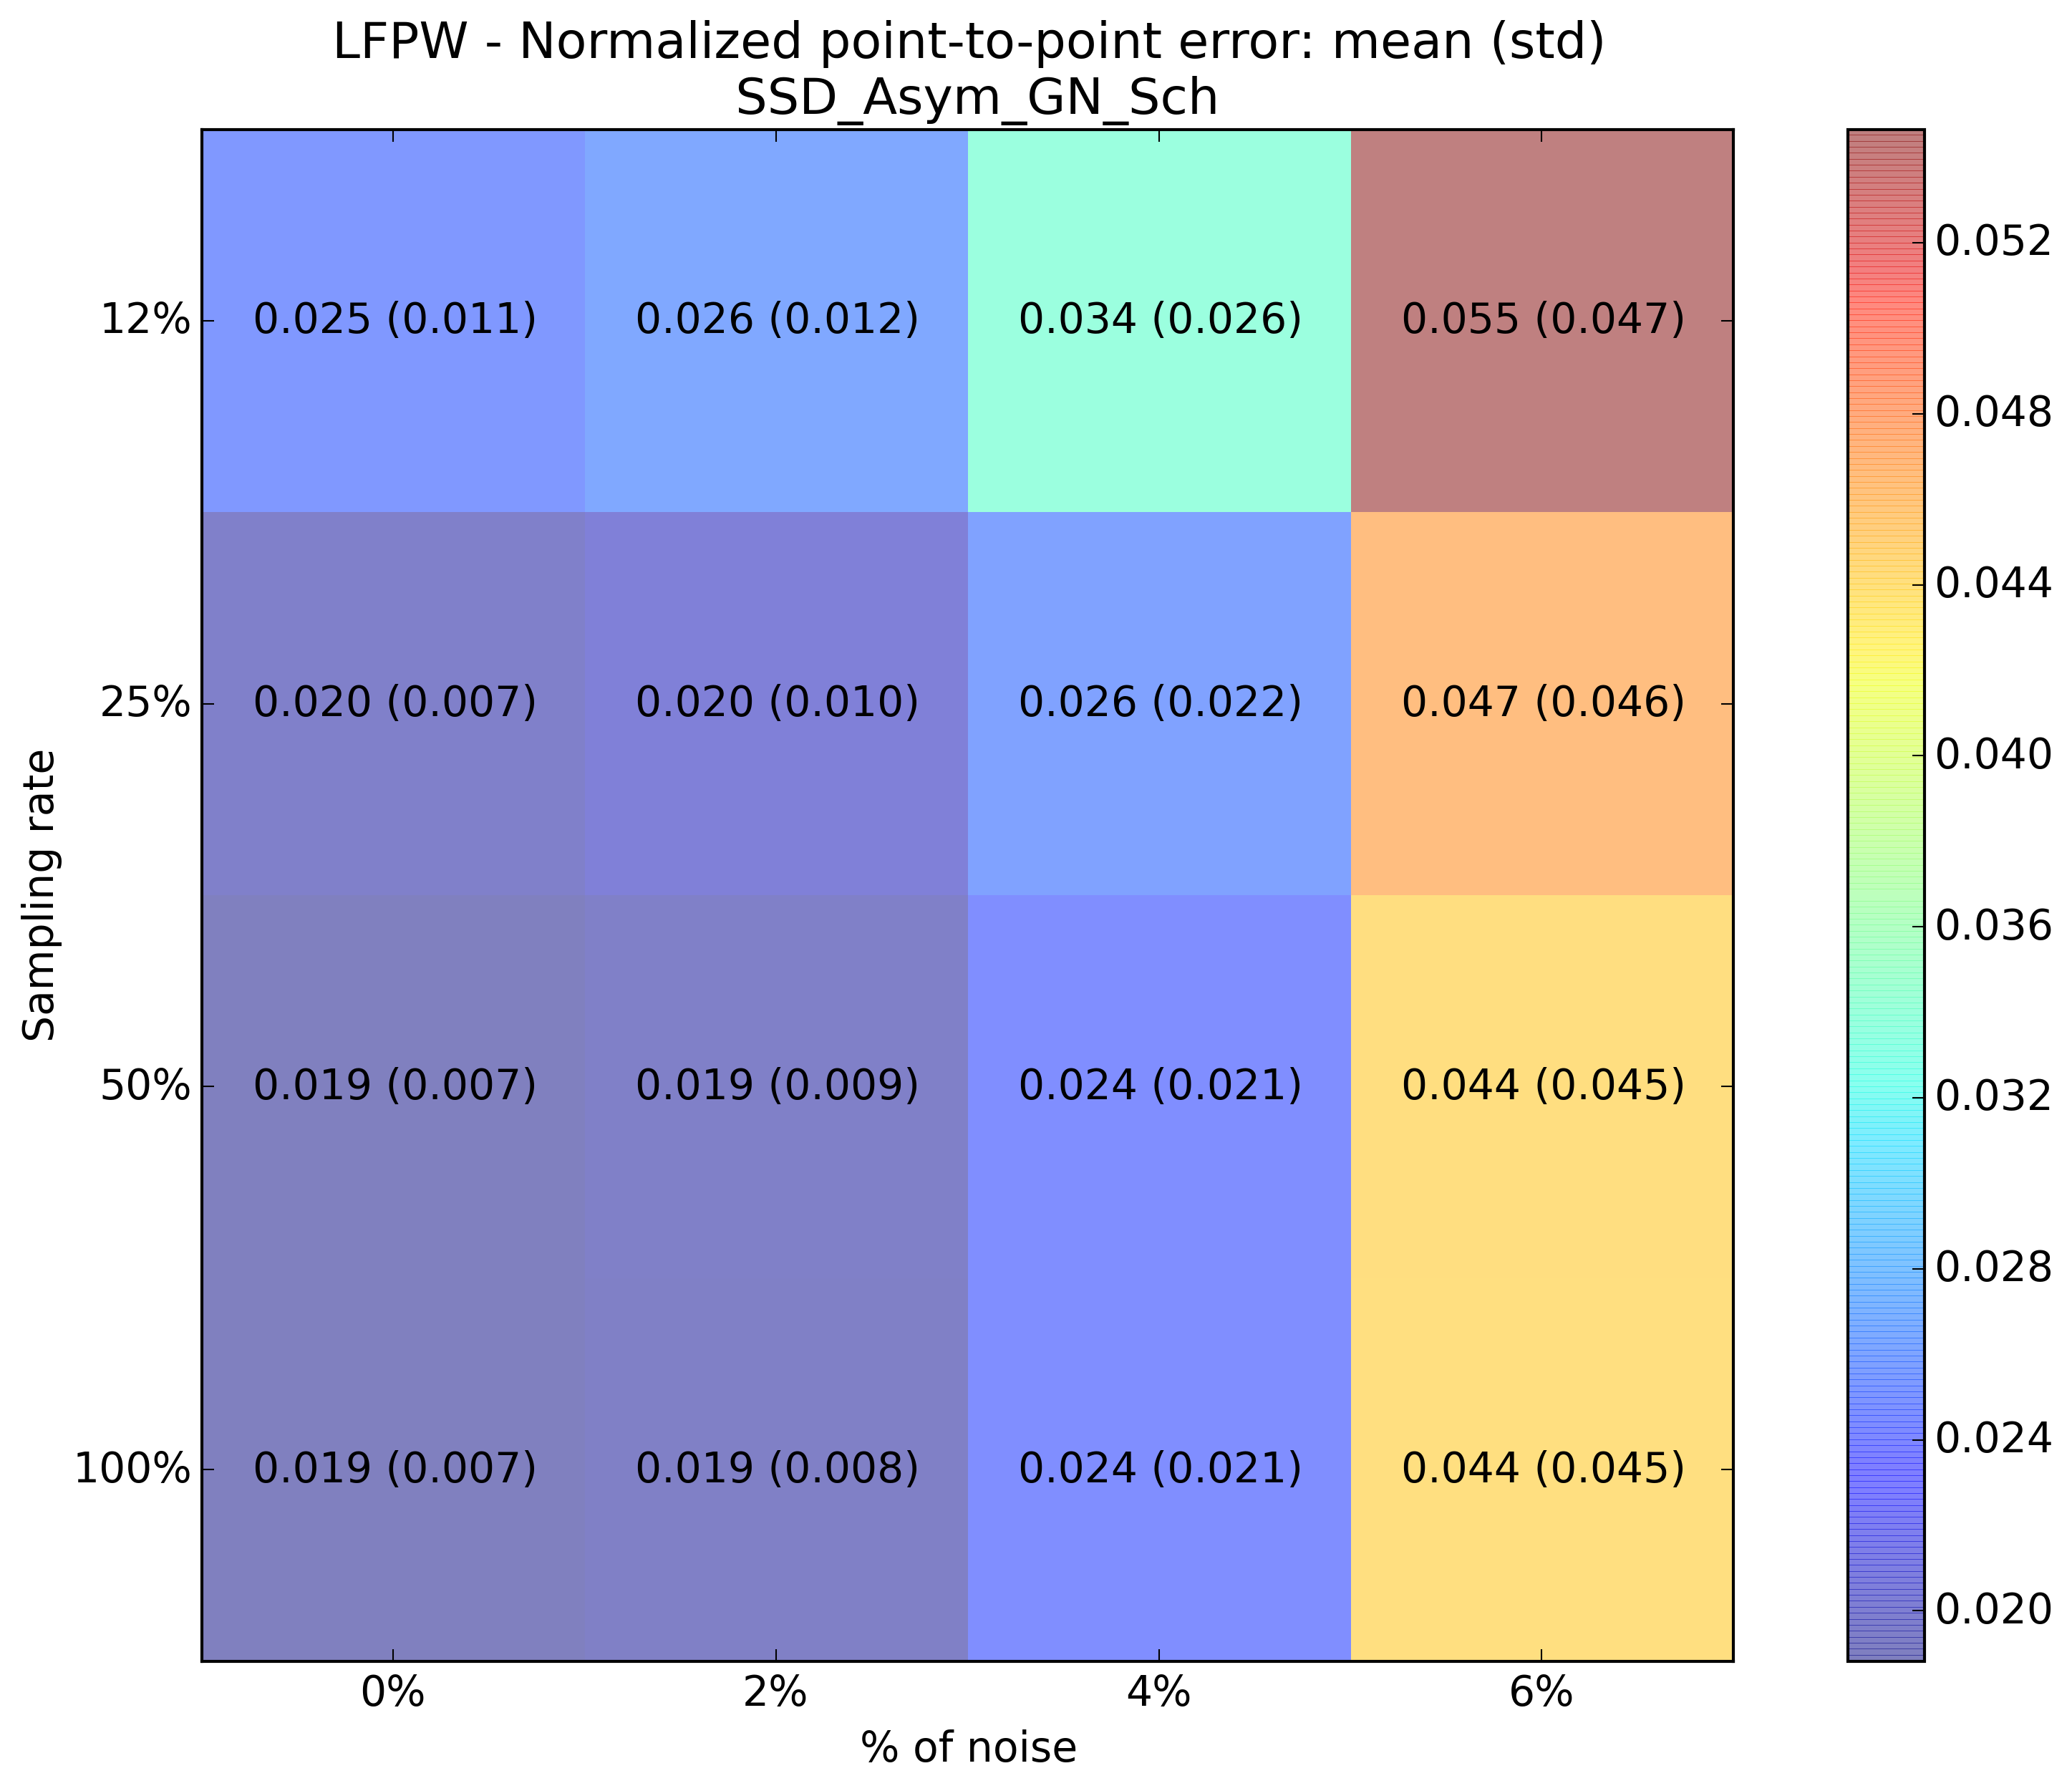
\includegraphics[width=0.45\textwidth]{experiments/sampling/ssd_asymmetric_gn/noise_vs_sampling_ssd_asymmetric.png}
    \caption{Mean and Std of normalized point-to-point error obtained on the LFPW test dataset by the SSD Asymmetric Gauss-Newton Schur algorithm for different sampling rates versus different amounts of noise \% on the initialization.}
    \label{fig:noise_vs_sampling_ssd_asymmetric}
\end{figure}

\begin{figure}[h!]
    \centering
    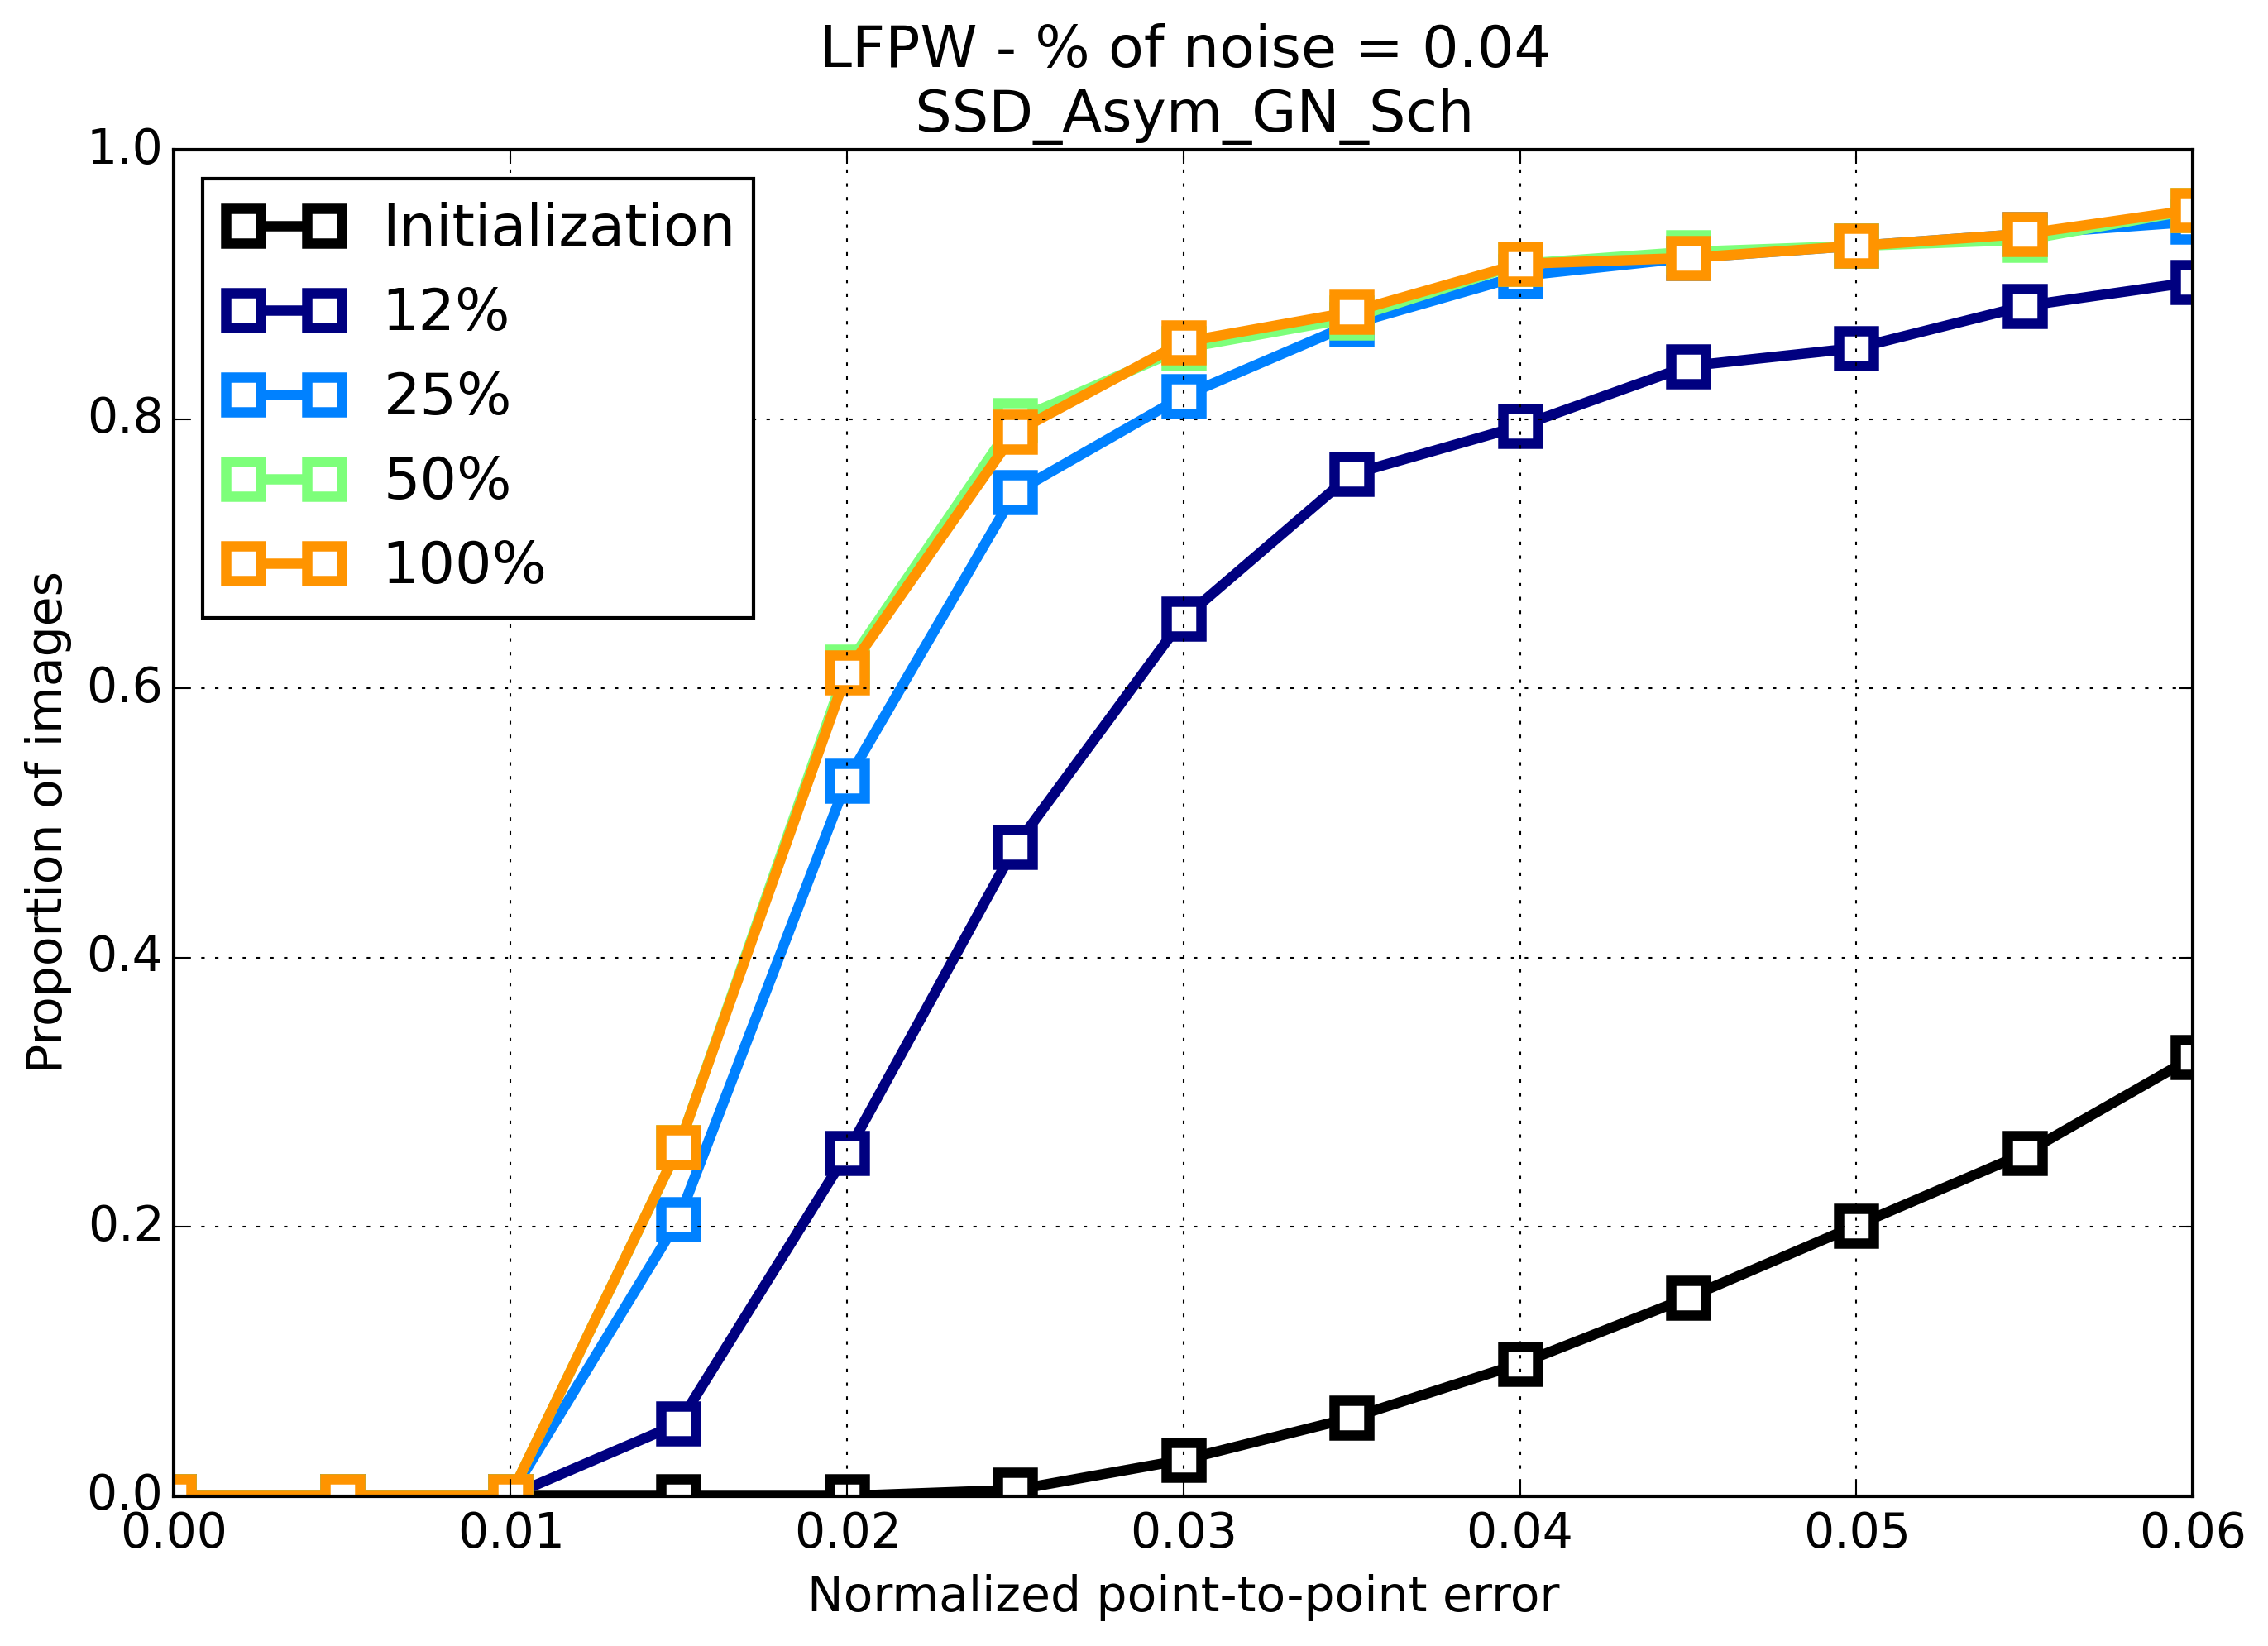
\includegraphics[width=0.50\textwidth]{experiments/sampling/ssd_asymmetric_gn/ced_ssd_asymmetric_gn_4.png}
    \caption{CED graph on the LFPW test dataset obtained by the SSD Asymmetric Gauss-Newton Schur algorithm for $4$\% noise on the initialization.}
    \label{fig:ced_ssd_asymmetric_gn_4}
\end{figure}

\begin{figure}[h!]
    \centering
    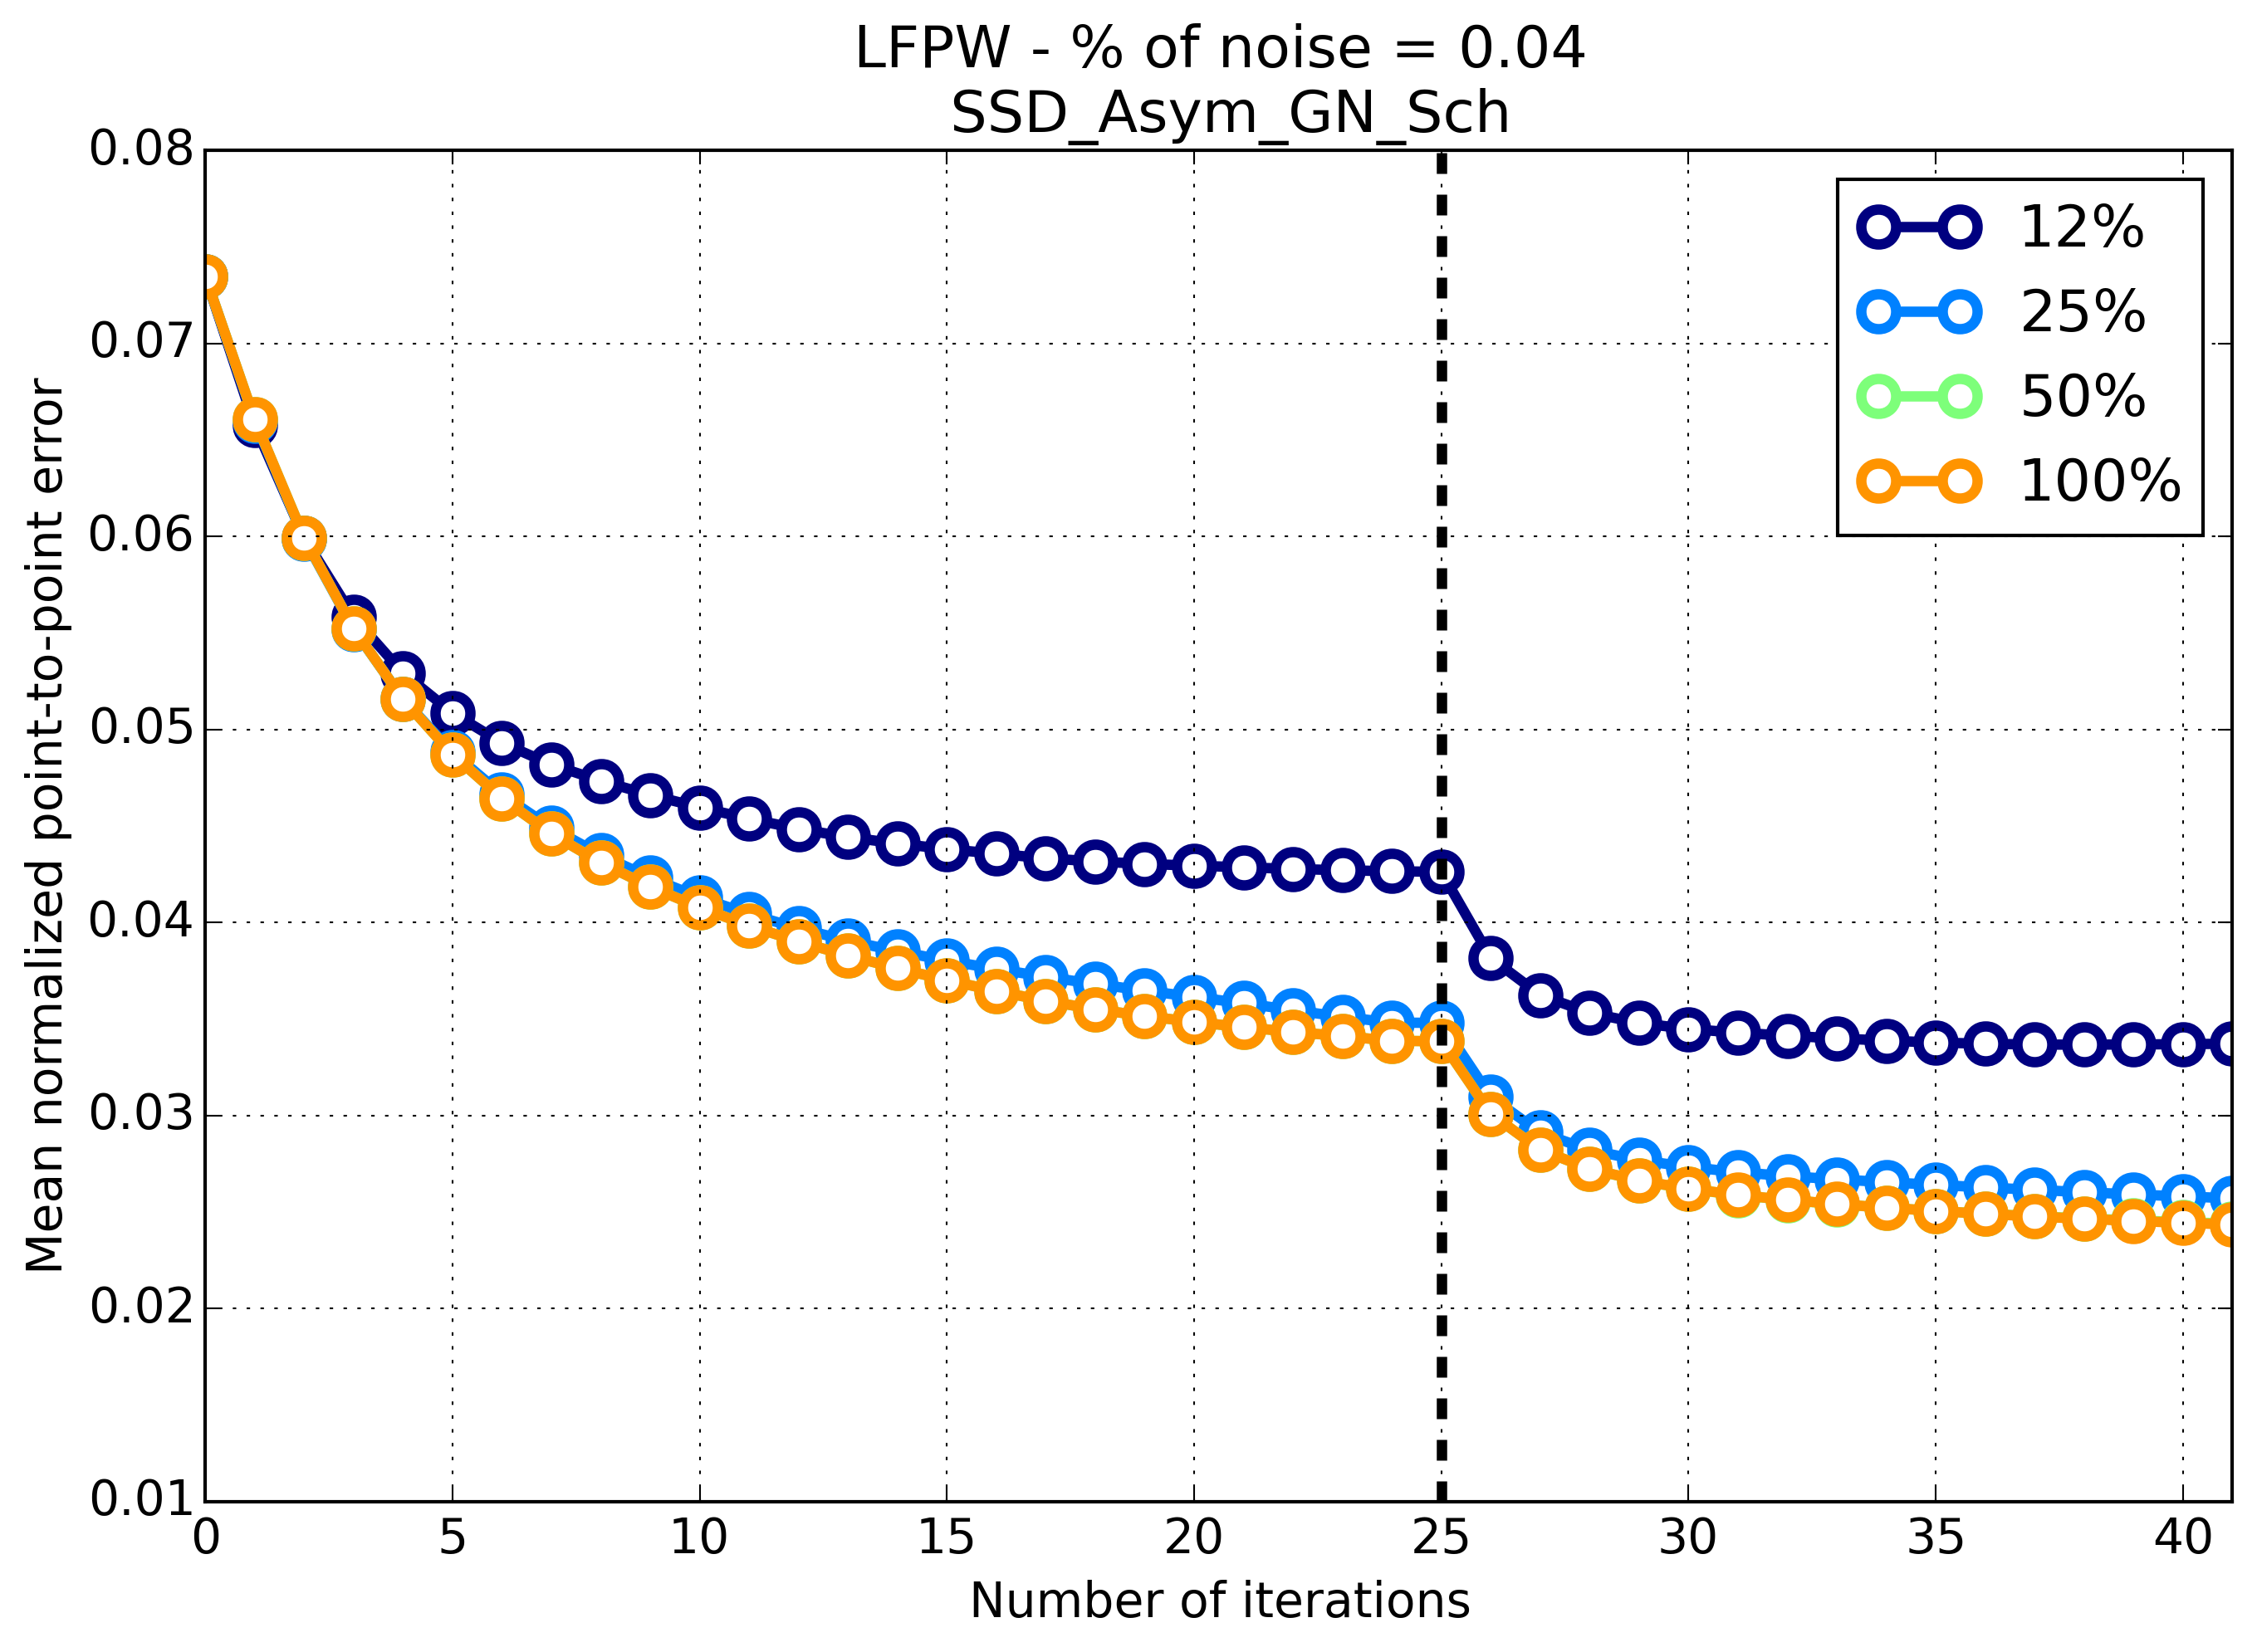
\includegraphics[width=0.50\textwidth]{experiments/sampling/ssd_asymmetric_gn/mean_error_vs_iters_ssd_asymmetric_gn_4.png}
    \caption{Mean normalized point-to-point error vs number of iterations graph on the LFPW test dataset obtained by the SSD Asymmetric Gauss-Newton Schur algorithm for $4$\% noise on the initialization.}
    \label{fig:mean_error_vs_iters_ssd_asymmetric_gn_4}
\end{figure}

\subsection{Comparison on Helen and AFW}





% This section reports the performance of the proposed method on the problem of face alignment in-the-wild. Results for two different experiments are reported. The first experiment compares the accuracy and convergence properties of the proposed Unified PIC-RLMS and AIC-RLMS algorithms with respect to those of PIC \cite{Baker2004}, AIC \cite{Papandreou2008} and and RLMS \cite{Saragih2011} on the popular LFPW \cite{Belhumeur2011} and Helen \cite{Le2012} datasets. The second experiment compares the performance of the previous algorithms against recently proposed state-of-the-art methods for face alignment in-the-wild, \ie the Supervised Descent Method of Xiong and De La Torre \cite{Xiong2013} and the Gauss-Newton Deformable Parts Model of Tzimiropoulos and Pantic \cite{Tzimiropoulos2014}, on the very challenging Annotated Faces in the Wild (AFW) dataset.

% \subsection{Comparison with AAMs and CLMs}
% Results for this experiment are reported over the 224 and 330 test images of the LFPW \cite{Belhumeur2011} and Helen\cite{Le2012} datasets. 66 points ground truth landmark annotations were provided by the iBUG group\footnote{\label{ibug_300}\url{http://ibug.doc.ic.ac.uk/resources/300-W/}}. All methods were initialized by perturbing the ground truth scale and translation parameters with Gaussian noise (rotations were not considered) and applying the resulting transformation to mean of the shape model. (Notice that this procedure produces initializations that are considerably more challenging than those reported in the recent AAM literature \cite{Tzimiropoulos2013, Tzimiropoulos2014}). The Cumulative Error Distributions (CED) for this experiment is shown in Figures \ref{fig:lfpw_exp1} and \ref{fig:helen_exp1}. Figures \ref{fig:lfpw_exp2} and \ref{fig:helen_exp2} shows the evolution of the mean normalized point-to-point error as a function of the number of iterations run by each algorithm. This experiment shows that our Unified AIC-RLMS approach considerably outperforms all other methods by a large margin on both datasets. More specifically, AIC-RLMS achieves a constant improvement of between 10\% to 20\% over PIC-RLMS and AIC at the significant region $0.020 < err > 0.040$ (at which the results are generally considered adequate by visual inspection). Note that the fast Unified PIC-RLMS algorithm is also the second most performant algorithm, surpassing both AIC and RLMS, on this particular experiment.

% \subsection{Comparison with state of the art}

% Results for this experiment are reported over the 337 images of the AFW \cite{Zhu2012} dataset. In this case, 49 points ground truth landmark annotations for this dataset were again provided by the iBUG group\footnoteref{ibug_300}. Results for \cite{Xiong2013} and \cite{Tzimiropoulos2014} were directly obtained using the publicly available models and fitting code kindly provided by the authors\footnote{\url{http://www.humansensing.cs.cmu.edu/intraface/}}$^{,}$\footnote{\url{http://ibug.doc.ic.ac.uk/resources/gauss-newton-deformable-part-models-face-alignment/}}. Note that, the provided models have been potentially trained using thousands of images in contrast to the only 813 images used to trained our method. In this experiment, all algorithms were initialized using the bounding box provided by our own in-house implementation of the face detector of \cite{Zhu2012}. The CED for this experiment are reported in Figure \ref{fig:afw_exp}. The results show that our Unified AIC-RLMS algorithm achieves state-of-the-art results on the AFW dataset, considerably outperforming both the Gauss-Newton Deformable Parts-Model of Tzimiropoulos and Pantic \cite{Tzimiropoulos2014} (which can be extremely accurate but sensitive to inaccurate initializations) and the SDM method of Xiong and De la Torre \cite{Xiong2013} (which can deal with very noisy initializations but is significantly less accurate than our method).

% \begin{figure}[t!]
% \centering
% \includegraphics[width=0.38\textwidth]{figures/graph7.png}
% \caption{Cumulative Error Distributions over 49 landmarks for the AFW dataset.}
% \label{fig:afw_exp}
% \end{figure}

\section{Conclusion}
\label{sec:conc}

%\begin{acknowledgements}
%If you'd like to thank anyone, place your comments here
%and remove the percent signs.
%\end{acknowledgements}

% BibTeX users please use one of
\bibliographystyle{spbasic}      % basic style, author-year citations
\bibliography{main.bib}   % name your BibTeX data base

\end{document}
